%%%%%%%%%%%%%%%%%%%%%%%%%%%%%%%%%%%%%%%%%%%%%%%%%%%%%%%%%%%%%%%%%%%
%                                                                 %
%   ZEBRA - Reference Manual -- LaTeX Source                      %
%                                                                 %
%   Main driver file. Includes other files of manual,             %
%   generates table of contents and includes index file.          %
%                                                                 %
%   Contains an description of the ZEBRA system                   %
%                                                                 %
%   Files referenced: zebfront.tex    front material              %
%                     zebintr.tex     introduction to zebra       %
%                     zebmz1 to 5.tex MZ reference section        %
%                     zebfz1 to 5.tex FZ reference section        %
%                     zebrz1 to 2.tex RZ reference section        %
%                     zebdz1 to 2.tex DZ reference section        %
%                     zebdzd1.tex     DZDOC reference section     %
%                     zebtz.tex       TZ Title handling           %
%                     zebjz.tex       JZ91 Processor support      %
%                     zebdia.tex      MZ and FZ diagnostics       %
%                     zebmza.tex      MZ appendix                 %
%                     zebrza.tex      RZ appendix                 %
%                     zebramain.bbl   bibliography information    %
%                                     uses cnasbibl.bib and       %
%                                          textproc.bib           %
%                     zebramain.ind   index made with MakeIndex   %
%                                                                 %
%   To run, you need the CERN style cernman.sty                   %
%                                                                 %
%   Editor: Michel Goossens / CN-ASD                              %
%   Last Mod.: 21 January 1997 16:20 mg                           %
%                                                                 %
%%%%%%%%%%%%%%%%%%%%%%%%%%%%%%%%%%%%%%%%%%%%%%%%%%%%%%%%%%%%%%%%%%%

\documentclass[11pt,dvips]{cernman}
\usepackage{longtable}
\usepackage{lscape}
%\usepackage[backref]{hyperref}
\setlongtables
\makeindex
\let\finalnewpage\clearpage
\setcounter{secnumdepth}{3}
\setcounter{tocdepth}{2}
\newcommand{\FZfile}{FZ~file\index{FZ!Sequential input/output}\index{input/output!FZ}}
\newcommand{\RZfile}{RZ~file\index{RZ!Random input/output}\index{input/output!RZ}}
\newcommand{\IQUEST}{\Lit{IQUEST}%
\index{IQUEST@{\tt IQUEST}!user communication vector in common {\tt QUEST}}%
\index{IQUEST@{\tt IQUEST}!error reporting}\index{error reporting!{\tt IQUEST}}%
\index{QUEST@{\tt QUEST}!user communication common}}
\newcommand{\QUEST}{\Lit{QUEST}\index{QUEST@{\tt IQUEST}|see{\texttt{IQUEST}}}}
\renewcommand{\ZEBRA}{\texttt{ZEBRA}}
\renewcommand{\Copt}[1]{\texttt{#1}}
\renewcommand{\Ropt}[1]{\texttt{#1}}
\renewcommand{\Rarg}[1]{\texttt{#1}}
\newenvironment{landscapebody}{\begin{landscape}}{\end{landscape}}
%\makeatletter
%\def\LS@rot{\setbox\@outputbox=\vbox{\@rotr\@outputbox}}
%\makeatother
\begin{document}
%  ==================== Front material ============================
%%%%%%%%%%%%%%%%%%%%%%%%%%%%%%%%%%%%%%%%%%%%%%%%%%%%%%%%%%%%%%%%%%%
%                                                                 %
%   ZEBRA DZ - Reference Manual -- LaTeX Source                   %
%                                                                 %
%   Front Material: Title page,                                   %
%                   Copyright Notice                              %
%                   Preliminary Remarks                           %
%                   Table of Contents                             %
%   EPS files     : cernlogo.eps, cnastit.eps                     %
%                                                                 %
%   Editor: Michel Goossens / CN-AS                               %
%   Last Mod.: 27 Jan 1995  9:00 mg                               %
%                                                                 %
%%%%%%%%%%%%%%%%%%%%%%%%%%%%%%%%%%%%%%%%%%%%%%%%%%%%%%%%%%%%%%%%%%%

%%%%%%%%%%%%%%%%%%%%%%%%%%%%%%%%%%%%%%%%%%%%%%%%%%%%%%%%%%%%%%%%%%%%
%    Tile page                                                     %
%%%%%%%%%%%%%%%%%%%%%%%%%%%%%%%%%%%%%%%%%%%%%%%%%%%%%%%%%%%%%%%%%%%%
\def\Ptitle#1{\special{ps: /Printstring (#1) def}
                       \epsfbox{cnastit.eps}}
\begin{titlepage}
\vspace*{-23mm}

\includegraphics[height=30mm]{cern15.eps}%
\hfill
\raisebox{8mm}{\Large\bf CERN Program Library Long Writeups Q100/Q101}
\hfill\mbox{}
\begin{center}
\mbox{}\\[6mm]
\mbox{\Ptitle{ZEBRA}}\\[2cm]
{\LARGE Overview of the ZEBRA System}\\[4mm]
{\LARGE MZ -- Memory Management}\\[4mm]
{\LARGE FZ -- Sequential Input/Output}\\[4mm]
{\LARGE RZ -- Random-access Input/Output}\\[4mm]
{\LARGE DZ -- Debugging Tools}\\[4mm]
{\LARGE DZDOC -- Bank documentation tools}\\[4mm]
{\LARGE TZ -- Title Handling}\\[4mm]
{\LARGE JZ91 -- Processor Support}\\[4mm]
{\LARGE Error Diagnostics}\\[25mm]
\end{center}
\vfill
\begin{center}\Large CERN Geneva, Switzerland\end{center}
\end{titlepage}

%%%%%%%%%%%%%%%%%%%%%%%%%%%%%%%%%%%%%%%%%%%%%%%%%%%%%%%%%%%%%%%%%%%%
%    Copyright  page                                               %
%%%%%%%%%%%%%%%%%%%%%%%%%%%%%%%%%%%%%%%%%%%%%%%%%%%%%%%%%%%%%%%%%%%%
\thispagestyle{empty}
\framebox[\textwidth][t]{\hfill\begin{minipage}{0.96\textwidth}%
\vspace*{3mm}
\begin{center}Copyright Notice\end{center}
\setlength{\parskip}{.6\baselineskip}

CERN Program Library entries \textbf{Q100} and \textbf{Q101}
 
\textbf{The ZEBRA system}

\copyright{} Copyright CERN, Geneva 1995
 
Copyright and any other appropriate legal protection of these
computer programs and associated documentation reserved in all
countries of the world.
 
These programs or documentation may not be reproduced by any
method without prior written consent of the Director-General
of CERN or his delegate.
 
Permission for the usage of any programs described herein is
granted apriori to those scientific institutes associated with
the CERN experimental program or with whom CERN has concluded
a scientific collaboration agreement.
 
Requests for information should be addressed to:
\vspace*{-.5\baselineskip}
\begin{center}\ttfamily
\begin{tabular}{l}
CERN Program Library Office              \\
CERN-CN Division                         \\
CH-1211 Geneva 23                        \\
Switzerland                              \\
Tel.      +41 22 767 4951                \\
Fax.      +41 22 767 8630                \\
Internet: cernlib@cern.ch
\end{tabular}
\end{center}
\vspace*{2mm}
\end{minipage}\hfill}%end of minipage in framebox
\vspace{6mm}
 
{\bf Trademark notice: All trademarks appearing in this guide are acknowledged as such.}
\vfill

\begin{tabular}{l@{\quad}l@{\quad}>{\small\tt}l}
{\em Contact Persons\/}: general        & Jamie Shiers /CN      & (shiers\atsign cern.ch)  \\
\phantom{\em Contact Persons\/}: FZ, MZ, TZ, JZ91 & Julius Zoll /ECP & (zoll\atsign cern.ch)  \\
\phantom{\em Contact Persons\/}: DZDOC  & Otto Schaile/PPE-Opal & (o.schaile\atsign cern.ch)\\[1mm]
\textem{Technical Realization\/}:       & Michel Goossens /CN   & (goossens\atsign cern.ch)\\[1cm]
\textem{Edition -- February 1995}
\end{tabular}
\newpage

%%%%%%%%%%%%%%%%%%%%%%%%%%%%%%%%%%%%%%%%%%%%%%%%%%%%%%%%%%%%%%%%%%%%
%    Introductory material                                         %
%%%%%%%%%%%%%%%%%%%%%%%%%%%%%%%%%%%%%%%%%%%%%%%%%%%%%%%%%%%%%%%%%%%%

\pagenumbering{roman}
\setcounter{page}{1}

\section*{Preliminary remarks}

This manual consists of several parts:

\begin{Itemize}
\item An overview of the ZEBRA system.
\item A reference section with a description of the DZ, MZ, FZ, 
      JZ91, RZ and TZ packages.
\item An example program showing how to use the MZ and DZ routines of ZEBRA.
\item A description of the DZDOC documentation system.
\item A list of the diagnostics messages generated by the FZ and MZ
      parts of the ZEBRA system.
\end{Itemize}

\subsection*{Conventions}

In this manual
examples are in \texttt{monotype face} and strings to be input by the user 
are {\Ucom{underlined}}.
In the index the page where a routine is defined is in {\bf bold},
page numbers where a routine is referenced are in normal type.

This manual flags output parameters in subroutine calls,
i.e. parameters which return values to the caller,
by an asterisk \Lit{"*"} following the argument's name.
If the input value of such a parameter is also significant
this is marked by prefixing a second asterisk.
A parameter which is a link is marked by an exclamation mark \Lit{"!"}.

The types of variables follow from the Fortran default typing
convention, except that variables beginning with the letters
"{\tt ch}" are of type {\tt CHARACTER}. 

The Fortran labelled \Lit{COMMON /\QUEST/IQUEST(100)} serves
for communication between the Zebra system and the user,
and also as scratch area in Zebra.

This document has been produced using \LaTeX~\cite{bib-LATEX}
with the \Lit{cernman} style option, developed at CERN. 
A gzipped compressed PostScript file \Lit{zebra.ps.gz}, 
containing a complete printable version
of this manual, can be obtained by anonymous ftp as follows
(commands to be typed by the user are underlined)%
\footnote{If you do not have the gnu {\tt gunzip} utility on your system
          you can get the uncompressed PostScript version by typing the
          command \Ucom{get zebra.ps}, without the {\tt gz} suffix. 
          In order to save Internet bandwidth, you are, however, strongly 
          urged to try and install the {\tt gunzip} utility since gzipped files 
          are about three times smaller than their unzipped equivalents.}:

\vspace*{3mm} 
\begin{XMP}
    \Ucom{ftp asisftp.cern.ch}
    Trying 128.141.201.136...
    Connected to asis01.cern.ch.
    220 asis01 FTP server (Version 6.10 ...) ready.
    Name (asis01:username): \Ucom{anonymous}
    Password: \Ucom{your\_{}mailaddress}
    230 Guest login ok, access restrictions apply.
    ftp> \Ucom{cd cernlib/doc/ps.dir}
    ftp> \Ucom{binary}
    ftp> \Ucom{get zebra.ps.gz}
    ftp> \Ucom{quit}
\end{XMP}
\vspace*{3mm} 

\newpage

%%%%%%%%%%%%%%%%%%%%%%%%%%%%%%%%%%%%%%%%%%%%%%%%%%%%%%%%%%%%%%%%%%%%
%    Tables of contents ...                                        %
%%%%%%%%%%%%%%%%%%%%%%%%%%%%%%%%%%%%%%%%%%%%%%%%%%%%%%%%%%%%%%%%%%%%
\tableofcontents
\listoffigures
\cleardoublepage
%\listoftables

% Local Variables: 
% mode: latex
% TeX-master: "zebramain"
% End: 

%  ==================== Body of text ==============================
\pagenumbering{arabic}
\setcounter{page}{1}
\part{An Introduction to the ZEBRA system}
%%%%%%%%%%%%%%%%%%%%%%%%%%%%%%%%%%%%%%%%%%%%%%%%%%%%%%%%%%%%%%%%%%%
%                                                                 %
%   ZEBRA User Guide -- LaTeX Source                              %
%                                                                 %
%   Chapter Introduction                                          %
%                                                                 %
%   The following external EPS files are referenced:              %
%   linstru , genstru , zeblink , bnkform , relocat               %
%                                                                 %
%   Editor: Michel Goossens / CN-AS                               %
%   Last Mod.: 29 Sep. 1993 20:30  mg                             %
%                                                                 %
%%%%%%%%%%%%%%%%%%%%%%%%%%%%%%%%%%%%%%%%%%%%%%%%%%%%%%%%%%%%%%%%%%%

\Filename{H1ZEBRA-An-overview}

\chapter{ZEBRA - An overview}

\Filename{H2Intro-Why-ZEBRA}
\section{Why ZEBRA?}

All off-line programming in high-energy physics is carried out, for
various reasons, in the Fortran~77 programming language. While this
language offers certain advantages over its competitors, it does suffer
from one serious defect, namely its lack of dynamic data structuring
facilities. The only data structures it contains at all are the array of
homogeneous elements and the common block for shared data. Neither of
these structures can be manipulated as an entity, and neither of them
can be defined dynamically at execution-time. No pointers are available
to link these structures together at a higher level.
If we were to attempt to
define structures using standard Fortran they would thus, at best, be in
the following style:

\begin{XMPt}{Example of defining data structure with Fortran}
      PARAMETER (NTRACKS = 100 , NPTS = 20)
      COMMON/POINTS/PTRACK(3,NTRACK),XYZ(NPTS,NTRACK),...
\end{XMPt}

and almost the whole program would have to be regenerated and recompiled
every time one of the symbolic constants is altered.
Relationships between data items would have to be programmed explicitly
using integer arrays of indices.
 
It is to overcome these limitations that the ZEBRA system has been
designed and written. It allows not only a truely dynamic
creation of data structures at execution-time, but also the added
advantage of being able to
{\bf manipulate} those structures, and even to write them to an external
storage medium and to recover them intact on some other computer.
In order to achieve this, the
user has to communicate with the ZEBRA system by (mostly) simple calls
to ZEBRA routines, and by following a number of rules and conventions.
Once a program has been written in this fashion, it becomes easy
for anyone knowing rather few of the details to use and to modify the
program, without having to worry about the side-effects of any changes
he or she makes, and without having to recompile large sections of the
code solely in order to obtain a few extra storage locations.
 
ZEBRA provides a significant extension to the power of Fortran, in
general at an insignificant cost in terms of execution-time overheads.
However, even that small cost is tiny compared with the extra time which
would otherwise be wasted in developing large programs using only the
conventional facilities.
 
The purpose of this chapter is to introduce the novice user to the basic
terms and concepts of ZEBRA. The actual use of the system
is described in later
chapters, where all the relevant information on calling sequences and so
forth is set out.

\Filename{H2Intro-Logical-Data-Structures}
\section{Logical Data Structures}
\subsection{The bank}

Imagine that we wish to store all the information about, say, a track in
a single unit, containing perhaps details of its momentum, direction,
coordinates etc. Using a call to the ZEBRA routine \Rind{MZBOOK}, we can ask
for an area of contiguous storage of a given length to be provided. The
actual location of this area is returned by \Rind{MZBOOK} as a
{\bf base address} which has to be used in all references to that area.
\index{bank}
This unit of storage is called a
{\bf bank}, and in Fortran code will be referenced as in:
\newpage
\begin{XMPt}{Addressing data words in a ZEBRA bank}
      Q(LTK+1) = PX
      Q(LTK+2) = PY
      etc.
\end{XMPt}
\Lit{Q}, by convention, is the name of the Fortran array underlying the
data structure, and \Lit{LTK} is the base address,
provided by \Rind{MZBOOK}, being the location of the word
preceding the first data word in the bank.
 
An advantage of ZEBRA is that it allows banks to contain data of
differing types. This is explained in detail later, but a simple
application would allow us to address another data word in the bank just
referenced as an integer, e.g.
\begin{XMPt}{Addressing integer data in a ZEBRA bank}
      IQ(LTK+19) = NPOINTS
\end{XMPt}
It is important to understand that for data structuring purposes
ZEBRA requires no knowledge of or control
over the actual contents of a bank. 
Whether it contains track data or a
list of family birthdays is not ZEBRA's concern. 
The internal details of
the data in a bank are solely the responsibility of the user(s), and it is
vital to maintain an adequate documentation of bank contents.
However, for input/output across computers and for printing
purposes, ZEBRA has to know the type of the bank contents, i.e. whether
the numbers are floating point, integer, Hollerith, etc.
This can be declared by a call to \Rind{MZFORM}.

\subsection{The linear structure}

In our example of a track bank, it is clear that in a given application
there may be a large and variable number of tracks to deal with.
To permit the realization of sets of objects of the same kind, ZEBRA
provides the construct of the {\bf linear structure} (figure \ref{LINSTRU}).
A linear structure consists of a series of linked banks, with each bank
holding in a reserved system word, called the {\bf next link},
the base address of the next member of the set. The next link of the
last bank of a linear structure has the value zero, indicating that
there is no next bank.
\index{link!next}
\index{data structure!linear}

\begin{minipage}{\textwidth}

\begin{Fighere}
\begin{center}
\mbox{\epsfig{file=linstru.eps,width=.9\textwidth}}
\end{center}
\caption{A simple linear structure}
\label{LINSTRU}
\end{Fighere}

\vspace*{-2mm}

\begin{XMPt}{Example of loop over linear chain}
      LTK = LFIRST                      ! Address of the first bank
   10 IF (LTK.EQ.0) GO TO finished      ! No next bank left ?
            .....                       ! Process data for the bank at LTK
          LTK = LQ(LTK)                 ! Get the address of the next bank
      GO TO 10                          ! Loop
\end{XMPt}
\end{minipage}

\newpage

The next link is stored in the word \Lit{LQ(LTK)} of the bank,
with the vector \Lit{LQ}
in offset EQUIVALENCE to the vector \Lit{Q} and \Lit{IQ}, as explained later.
The example above shows the ZEBRA equivalent of a Fortran DO-loop to process
all the banks of a linear structure.

Banks are created dynamically at execution time, and because each
bank has one word to connect the rest of the structure of which it is a
member, the linear structure permits the creation at
execution time of sets of an arbitrary number of objects,
independent of any declaration of maximum dimension, either at
execution time or at compile time, as would be the case with Fortran
arrays.

The order of the banks in a linear structure, although defined, is not
normally significant. It depends on the details of the creation process,
as will be seen later. The user may, however, associate significance to
the defined order, and ZEBRA utilities are provided to re-order the
banks in a linear structure by re-arranging the next links (\Rind{ZSORT}).

It will be necessary to refer to the
``address of a linear structure''.
This is simply the base address of its first bank. If this address is
available, all the banks of the linear structure can be reached.
\subsection{The general data structure}
\index{data structure!general}
\index{link!down}

In the general case, more complex structures are needed than the linear
one just described. 

\begin{Fighere}
\begin{center}
\mbox{\epsfig{file=genstru.eps,width=\textwidth}}
\end{center}
\caption{An example of a general structure}
\label{GENSTRC}
\end{Fighere}

For instance, in the context of a high-energy
physics program a number of track banks may depend on a bank at a
logically higher level which
describes a track vertex. 
This vertex bank will
contain a link to the first of the track banks. 
Such a link is called a {\bf down} link.
It is possible for a given bank to have a large number of
down links, and for it to depend similarly on a logically yet higher bank
through a down link in that bank.
We thus see that the down links allow the construction of
a tree structure, and that at each node there may be either a
single bank or a linear structure. This may be pictured as in
Figure~\ref{GENSTRC}.

All the links so far described are stored by ZEBRA as part of the bank
concerned. We note that the down and next links are referred to collectively
as {\bf structural} links, as they represent the basic connections
of a data structure.

\subsection{Reverse links}

Each ZEBRA bank contains a link pointing to the bank on which the
whole linear structure of which it is a member depends. 
This is called the {\bf up link}. 
The value of this link is zero if the bank concerned is 
itself at the top of the tree structure.
Finally, each bank has also an {\bf origin} link, which points
to the structural link supporting the bank.
The up link and the origin link are known as {\bf reverse} links.
A summary of the four types of links known to ZEBRA is given in
Figure \ref{ZEBLINK}\index{link!reverse}
\index{link!origin}
\index{link!up}

\subsection{Reference links}

The links so far described are an integral part of the data structure
which they represent. It often happens that a user wishes to establish
links between various banks which are not part of the structure itself,
but merely references that the user wishes to record.
These are then known as
{\bf reference links}. A bank can contain a large number of such links,
and their use is at the discretion of the user, and entirely his
responsiblity. For the reference links the task of
the ZEBRA system is limited to changing their
values in the event that, for reasons to be explained
below, banks have to be moved, or relocated, in memory. Reference links
provide a high level of generality in the design of complete data
structures, and are another of those features which so greatly
enhances the power of Fortran.

\begin{Fighere}
\begin{center}
\mbox{\epsfig{file=zeblink.eps,width=\textwidth}}
\end{center}
\caption{A schematic overview of the links known to ZEBRA}
\label{ZEBLINK}
\end{Fighere}

\Filename{H2Intro-Physical-Storage}
\section{Physical Storage}

It is clear that somehow the banks just described have to be mapped on
to physical computer storage, or memory.
This is achieved in ZEBRA by declaring to the system one or more common
blocks which are to provide the actual storage for the data structures.
It is often sufficient for off-line programs to declare a single large
common block; it is for on-line applications, or for certain large
off-line applications that the possibility to define several distinct
blocks is foreseen. A typical declaration has the following form:
\newpage
\begin{XMPt}{Declaration of the ZEBRA storage}
      COMMON /MYSTOR/ IFENCE(10),LINKS(10),LINKR(20),ISTORE(10000)
      DIMENSION     LQ(999),IQ(999),Q(999)
      EQUIVALENCE  (LINKS(9),LQ(9),IQ(1),Q(1))
\end{XMPt}
An actual common block is declared to ZEBRA by a call to \Rind{MZSTOR},
and in ZEBRA is termed a {\bf dynamic store}.
The actual layout of memory in a store declared by the example above is shown
in figure \ref{FMZSTOR}.

\begin{Fighere}
\begin{center}
\mbox{\epsfig{file=mzstor.eps,width=\textwidth}}
\end{center}
\caption{The layout of the ZEBRA default store}
\label{FMZSTOR}
\end{Fighere}

Within the common block just described, we notice that the effect of th
\Lit{EQUIVALENCE} statement is to offset the arrays \Lit{Q} and 
\Lit{LQ} by eight locations. 
This permits in the references to the data words and to the
links a simple form of subscript, namely that each data word is
addressed as \Lit{Q(L+n)}, 
as already seen, and that each link is referenced as \Lit{LQ(L-m)}. 
This may be better appreciated by studying the layout of an
actual bank, whose layout is detailed in Figure~\ref{BNKFORM},
where the various sections of the bank may be seen, in particular the
data and the links.

\begin{figure}[p]
\begin{center}
\mbox{\epsfig{file=bnkform.eps,width=\textwidth}}
\end{center}
\caption{The format of a ZEBRA bank}
\label{BNKFORM}
\end{figure}

The total number of links \Lit{NL} plus a constant plus the number of the
optional, so-called extra I/O words, stored
in the lower part of the first word of the bank (see below),
is required to step over the link
region to reach the central area during a sequential scan
through the store.
The upper part of the first word contains the I/O control-byte.
Together with the extra I/O words, if any, it constitutes the
``I/O characteristic'', describing the nature of the bank contents,
as needed for conversion if the bank is written to a file for reading
on some other computer, and also for interpretative dumps
(see the description of routine \Rind{MZFORM}).
\index{bank!I/O characteristic}
\index{link!next}
\index{link!up}
\index{link!origin}

The central part of the bank starts with the next link,
accessed as \Lit{LQ(L)}.
The up link at \Lit{LQ(L+1)} points to the header bank supporting
the linear structure of which the bank is a member;
it is zero if the bank is a primary header bank.
The origin link at \Lit{LQ(L+2)} points to the link
through which the bank is reached.
The origin link is not usually of interest to the user,
its sole purpose is to free the user from having to remember the
supporting link. These three links, next, up and origin are present
in every bank and are not counted in \Lit{NL} and \Lit{NS}.
\index{bank!identifier!numeric}
\index{bank!identifier!Hollerith}

The two words \Lit{IQ(L-5)} and \Lit{IQ(L-4)} contain the numeric and Hollerith bank
identifiers, \Lit{IDN} and \Lit{IDH}. 
Usually all the banks of a linear structure
have the same \Lit{IDH}, but different \Lit{IDN}'s to permit ready
identification of a particular bank in interactive work.
Words \Lit{IQ(L-3)} and \Lit{IQ(L-2)}
hold the total number of links (\Lit{NL}) and the number of structural
links (\Lit{NS}), respectively,
and word \Lit{IQ(L-1)} holds the number of data words (\Lit{ND}).

The status word at \Lit{IQ(L)} provides in positions
1 to 18 for user status bits,
while positions 19 to 32 are reserved for system use. In particular
bits 19 to 22 contain the number of extra I/O descriptor words \Lit{NIO},
needed to go backwards from the centre to the start of a bank.

With this format the smallest possible, but useless, ZEBRA
bank (\Lit{NL=NS=ND=0}) occupies 10 words.

\subsection{Divisions}
\index{division}

So far we have seen how banks are stored in a dynamic
store. In fact, a dynamic store may physically be subdivided into
{\bf divisions}. The purpose of the division is to enable ZEBRA to
manipulate groups of logically associated banks efficiently, for instance
for input-output or for dropping banks, and also to allow it to handle links
more efficiently when it knows that they are restricted to a single
division.

When a store is initialized by \Rind{MZSTOR}, it automatically creates three
divisions, one for itself and two for the user. Further divisions may be
created explicitly by a call to \Rind{MZDIV}.

It should be noted that stores and divisions are identified by
means of a store/division index whose value never changes. These indices
should be maintained in, for instance, the common block to which they
refer, for reasons of
data integrity.

\subsection{Link areas}
\index{link!area}

It is possible for a user to store bank addresses or links, for ease
of manipulation, in a user-defined area, or {\bf link area}.
These should be kept in a common block, and a call to
\Rind{MZLINK} or \Rind{MZLINT} is necessary to declare these areas to ZEBRA, which
will then maintain them in the event of a bank relocation. For this
reason, the link areas associated with different stores have to be kept
separately.

\subsection{Working space}
\index{working space}

It happens frequently in a program that some temporary working space is
required, perhaps for use within one or two routines. 
ZEBRA permits a user to ask for such working space by a call to \Rind{MZWORK}. 
The necessary
storage is made physically available at the beginning of the relevant
store, and may contain reference links and data. It should be noted that
the first division in the store is logically part of the working space,
and its existing contents are destroyed by a call to \Rind{MZWORK}. 
Normally, therefore, the first division should itself be used only for 
banks which are very short term.

\newpage
\Filename{H2Intro-Dropping-banks-and-garbage-collection}
\section{Dropping banks and garbage collection}

Initially a dynamic store is empty, except for a few system banks in the
system division. As banks are created the occupied space increases and
the free space decreases. 
By calling \Rind{MZDROP} the user may {\bf drop}
banks, which are not needed any longer. 
\Rind{MZDROP} logically removes banks,
or whole sub-structures, from the surrounding data structure and marks
the banks as dropped. These dropped banks stay intact in memory and in
particular, reference links pointing to dropped banks continue to point
to valid information.
\index{garbage collection}

Possibly, but not normally, the situation can arise, that the free space
is not sufficient to satisfy a request for creating a bank, in which case
ZEBRA will recuperate the space occupied by the dropped banks. 
This operation, called {\bf garbage collection}, moves the active
banks of
a division to form one contiguous area, squeezing out the dropped banks
and thereby increasing again the free space, updating all links for the
new positions of the banks in memory, including a reset to zero of
reference links which used to point to the dropped banks which have now
disappeared. The process of changing the links for the new position in
memory is called {\bf relocation}.
\index{relocation}

ZEBRA triggers a garbage collection automatically whenever a request
for memory cannot be satisfied. If even after garbage collection there
is not enough space, \Rind{MZBOOK} etc. will take an error exit and thus the
user does not have to test, after each call to \Rind{MZBOOK} etc., for the
successful completion of the request.

For garbage collection the ZEBRA system has to know the whereabouts of
{\bf all} the links in the program. 
For this reason it
is essential that the user keeps all bank addresses in locations known
to ZEBRA, either in the link part of banks, or in the link part of the
working space or in link areas. 
Any link kept elsewhere will be invalid after a garbage collection.
 
The memory move involved in a garbage collection is represented in
Figure~\ref{RELOCAT}.

\vspace*{-5mm}
\begin{Fighere}
\begin{center}
\mbox{\epsfig{file=relocat.eps,width=\textwidth}}
\end{center}
\caption[The layout of memory in a division before and after garbage
         collection.]%
        {The layout of memory in a division before and after garbage
collection.\\ The top part of the picture
shows a number of ``live'' banks numbered 1 to 7
and 5' to 1', which interspersed ``dead''
banks (i.e. banks whose information is no longer needed and whose space
can hence be recovered).
The bottom part of the picture shows the same ``live''
banks which have been left justified to increase the free space.}
\label{RELOCAT}
\end{Fighere}

\newpage
\Filename{H2Intro-Wiping-divisions}
\section{Wiping divisions}

In high energy physics repetitive ``event processing''
is a very common
situation: event-by-event the data are read, processed, output and
dropped. Each event is represented by one or several data structures,
which disappear completely before the next event is dealt with.
In this situation it would be inefficient to drop the event with \Rind{MZDROP}
and to rely on garbage collection to recover the space of the previous
event only later, maybe at the moment when the data volume of the new
event is already substantial and would have to be copied. It is much
more efficient to separate the short term data of the event from the
long term data (data held by the program over many events), by
directing them into separate divisions. The event can then be
abandoned with \Rind{MZWIPE} which resets one or several divisions to be empty,
thereby freeing the space for immediate re-use.

\Filename{H2Intro-Input-Output}
\section{Input/Output}

One of the important features of ZEBRA is its ability to handle the
transfer of data structures to and from an external medium. 
This is performed by calls to routines in the FZ part of the
\index{FZ!Sequential input/output}\index{input/output!FZ}%
system, and the user does not need to program any explicit Fortran input/output
statements. 
But the power of the system goes beyond that of a simple data transfer. 
It is able to maintain the integrity of a data structure
between an output operation and a subsequent input operation by
appropriate changes to the values of the links connecting the structure. 
In addition, ZEBRA permits input/output to either sequential or direct 
access files, depending on the nature
of the data and, very important, it also provides two modes of data
representation. 
\index{FZ!Sequential input/output!native mode}%
The first is called {\bf native} mode, and implies that the data 
undergo no conversion when
transfered between storage and the external medium. Such data may be read
only on a computer of a compatible architecture. 
The {\bf exchange} mode, on the other hand,
\index{FZ!Sequential input/output!exchange mode}%
allows transfer of data between a large variety of
computers by making appropriate conversions to and from an interchange
format.
                                          
On the other hand the ZEBRA RZ package permits the storage and retrieval of 
ZEBRA data structures or Fortran vectors in random access files. 
Files may reside on standard
direct access devices such as magnetic disk, or be
mapped to virtual memory. 
\RZfile s can be accessed by several users simultaneously,
even across networks.
Remote file access and transfer is provided for RZ files
using standard tools, such as NFS and ftp. In the heterogeneous
environment, the tools provided in the CSPACK~\cite{bib-CSPACK} 
package may be used.

The RZ package is not a relational database management system,
but organises data in a hierarchical manner which is suitable
for many applications in High Energy Physics, and probably outside.


\newpage
\Filename{H2Intro-Debugging-problems}
\section{Debugging problems}
\subsection{The debugging and documentation package}

It is inevitable that errors will sometimes be made in constructing and
manipulating the data structures supported by ZEBRA. 
In order to allow
a simple and convenient means of checking the integrity of the structures,
including the links and the data, the DZ package has been provided
(see chapter \ref{sec:dzdescription}).
It has various options to display and validate the whole or part of a dynamic
store.

The DZDOC package contains routines for generating and maintaining documentation
on ZEBRA data structures (see chapter~\ref{sec:dzdocdescription}).

\subsection{The user communication array {\tt IQUEST}}

Information about problems or important input/output running
parameters is available in the user communication array 
\IQUEST{} in common \Lit{/\QUEST/}. 
In order to have access to the information in this array
the user should include the following definition in his code:
\begin{XMPt}{Fortran definition of the user communication vector \Lit{IQUEST}}
      COMMON /QUEST/IQUEST(100)
\end{XMPt}
When a routine detects an error, it identifies itself and gives the
case number describing the problem. 
This number, together with the
detailed description of the contents of the \IQUEST{} elements, will allow
the user to trace the problem.

In the case of input/output routines (i.e. the FZ and RZ packages)
information about the last operation is available via \IQUEST{}
(see the description of each routine for the meaning of individual 
\IQUEST{} values).

\Filename{H2Intro-Some-conventions}
\section{Some conventions}

ZEBRA uses certain conventions,
for instance that the second letter of each routine or common block
name is a \Lit{Q} or \Lit{Z}. 
For this reason, users are urged not to
write common block or routine names which could be confused with ZEBRA
names, by avoiding these two letters in that position. 
Users are also
recommended to begin all link names with an \Lit{L}, in order that this become
a common convention, thereby improving the readability of programs.

\Filename{H2Intro-Summary}
\section{Summary}

This chapter has tried to set out the basic features of ZEBRA, together
with a justification for attempting to increase the power of the
programming facilities available to a programmer in this way. The nature
of the data structures has been described, together with the manner
in which they
can be manipulated, displayed, and written and read.

The ZEBRA system has been developed, in part, because of weaknesses in
Fortran 77. 
The new language standard Fortran~90 provides high level data structure
constructs, whose impact on high-energy physics programming are being
investigated.
Until then, high-energy physicists are able
to develop data structures, one of the most important parts of
programming, using ZEBRA.

\part[MZ -- Memory Management]%
     {MZ -- Memory Management\\[5cm]%
      {\LARGE Package written by J. Zoll/ECP}\\[1cm]
      {\LARGE Package maintained by H. Meinhard/ECP}}
% 13 November 1993 mg
\Filename{H1-MZ-memory-management}
\chapter{Memory management}
\label{sec:H1-MZ-memory-management}

The memory management package MZ of ZEBRA is fundamental
to all other ZEBRA packages.

The ZEBRA package MZ derives from its predecessors:

\begin{itemize}
\item the ZEBRA data structure derives from the HYDRA data structure~\cite{bib-HYDRAMZ};
\item the multi-store strategy derives from ZBOOK~\cite{bib-ZBOOK}
\end{itemize}

\Filename{H2-MZ-ZEBRA-bank-format}
\section{ZEBRA bank format}

\begin{verbatim}
    LQ(L-NL-NIO-1) IOcb/NOFF    IOcb: I/O control byte (16 bits)
                                NOFF = NIO + NL + 12 (16 bits)

    LQ(L-NL-NIO)   IOW (1)      first extra I/O descriptor word (if any)
                   ...
    LQ(L-NL-1)     IOW (NIO)    last  extra I/O descriptor word

    LQ(L-NL)       link NL      last reference link
                   ...
    LQ(L-NS-1)     link NS+1    first reference link
    LQ(L-NS)       link NS      last structural link
                   ...
    LQ(L-1)        link 1       first structural link

    LQ(L)          next         adr of the next bank in the linear str.
    LQ(L+1)        up           adr of the supporting bank
    LQ(L+2)        origin       adr of the supporting link

    IQ(L-5)        IDN          numeric   bank ID
    IQ(L-4)        IDH          Hollerith bank ID  (4 characters)
    IQ(L-3)        NL           number of links
    IQ(L-2)        NS           number of structural links
    IQ(L-1)        ND           number of data words

    IQ(L)          status       bits  1-18 user
                                     19-32 system   25: drop bit
                                     19-22 NIO      26: mark bit
    IQ(L+1)        first data word
                   ...
    IQ(L+ND)       last  data word

            This layout requires:

                  DIMENSION    LQ(999), IQ(999), Q(999)
                  EQUIVALENCE (LQ(9),IQ(1),Q(1))


 ---- Format of a short dead region ----

    word 1:  bits  1-16: NW, # of words, with  0 < NW < 12
                   17-24: NW again for redundancy
                      25: drop-bit set
                  26-end: zero
     2->NW:  dead words, content irrelevant
\end{verbatim} 

\Filename{H2-MZEBRA}
\section{MZEBRA - initialize the ZEBRA system}

To initialize the ZEBRA system Common blocks the user must call
\Rind{MZEBRA}, before any other request to ZEBRA.

In particular, the following COMMON variables of interest to
the user are initialized:

\begin{verbatim}
logical unit numbers:
      COMMON /ZUNIT/ IQREAD,IQPRNT,IQPR2,IQLOG,IQPNCH,IQTTIN,IQTYPE

default logging level:
      NQLOGD in /ZSTATE/

where
      IQREAD   lun for standard system input ('card reader')

      IQPRNT   lun for standard  user print output
      IQPR2    lun for secondary user print output
               initialization: IQPRNT=IQPR2=IQLOG

      IQLOG    lun for standard system output ('line printer')
               this is used for all ZEBRA system printing

      IQPNCH   standard system coded output to be read back by
               program ('card punch')

      IQTTIN   standard on-line terminal input  (zero if none)
      IQTYPE   standard on-line terminal output (zero if none)

      NQLOGD   system-wide default logging level, see next para.
               standard default initialization to zero
\end{verbatim} 

On any particular machine ZEBRA knows the correct values for
the logical unit numbers, for example it knows that 6 and 7
are the right values for \Lit{IQREAD} and \Lit{IQLOG} on the IBM,
similarly  \Lit{L"INPUT"} and \Lit{L"OUTPUT"}  on the CDC Cybers.
It is of advantage to the user to direct all his print output
through the unit numbers provided by ZEBRA in \FCind{/ZUNIT/}.
After the call to \Rind{MZEBRA} he is free to change any particular
value in \FCind{/ZUNIT/}, and with the call to \Rind{MZEBRA} he may also
modify the initialization, in particular he may re-direct
the standard print output to the on-line terminal.

The parameter in the call to \Rind{MZEBRA} may select initialization
options either with an integer constant or with a list:

\Shubr{MZEBRA}{(LIST)}

\begin{verbatim}
 --- short form of options:

   with  LIST = 0:  standard defaults
               -1:  preset IQLOG = IQTYPE, ie. output to terminal
               -2:  preset NQLOGD= -2,     ie. only error messages
               -3:  preset NQLOGD= -2 and IQLOG=IQTYPE

\end{verbatim}

\begin{verbatim}
 --- options specified by a list:

   with  LIST(1)   N elements in the list to follow (excluding itself)
                   if zero or -ve: standard options

             (2)   -> NQLOGD, the system-wide default log level
                              (see MZLOGL on the next page)

                   for example: LIST(2)= -3: suppress all messages
                   standard default: NQLOGD = 0

             (3)   -> IQLOG,  lun for standard log printing
                              unless absent or zero
                              if = -1: set IQLOG = IQTYPE

             (4)   -> IQPRNT, lun for standard output printing
                              if absent/zero: set IQPRNT = IQLOG
                              if = -1:        set IQPRNT = IQTYPE
\end{verbatim} 

\Shubr{MZVERS}{}

 prints at logging level -1 or above an initialisation message
on unit \Rarg{IQLOG}, showing amongst other things,
the version number of the current ZEBRA system.
In \Lit{\IQUEST(1)} it returns as an integer
the Zebra MZ version number multiplied by 10000;
thus version 3.66 /7 would give 36607.

\Examples

\begin{verbatim}
   set normal logging, set printer output to terminal:

      CALL MZEBRA (-1)
      CALL MZVERS

   set monitor logging, set unit 4 as print file:

      DIMENSION    LIST(3)
      DATA  LIST   / 2,  2, 4 /
      CALL MZEBRA (LIST)
      CALL MZVERS
\end{verbatim} 

\Rind{MZEBRA} only initializes the general ZEBRA system commons,
it does not initialize the dynamic store.
Before any request to the ZEBRA system involving the store,
the user must initialize it by calling \Rind{MZSTOR}.

\Shubr{MZEND}{}

Should be called at the end of execution by the user
to obtain the statistics of usage of the dynamic store.

\Filename{H2-MZLOGL}
\section{MZLOGL - change the MZ logging level}

Various parts of the ZEBRA system write log messages
to the standard system output,
and occasionally also to the on-line terminal, if any.
Examples of messages provided for are:

\begin{verbatim}
   a) messages for recoverable errors:
      read errors, data errors

   b) intialization messages for:
      stores, divisions, link areas, files

   c) termination messages giving statistics of usage of
      various facilities like memory, files

   d) operation messages:
      change in program phase, end-of-file

   e) watch messages for hopefully rare, expensive events:
      garbage collection, MZPUSH with relocation

   f) monitor messages to help the user debug his program
\end{verbatim} 

To control the amount of information thus provided to the user,
a log level is defined and can be set and reset by the user
at execution time.
The default log level zero enables the messages which one would
usually like to see for record in a production run.
The user may reduce the log level to cut out most or all messages;
he may increase the level to watch the running of his program,
or even to debug his data or his input files.

Separate ZEBRA entities, such as dynamic stores or files,
each have their own attached log level,
which may be changed by the user at any time.
By default they inherit the global system-wide default log-level
set by \Rind{MZEBRA}, whose own default is zero.

A somewhat similar system has been used
for the debugging of the ZEBRA system itself;
the corresponding WRITE statements are still present in the code
on the PAM files, although not on the object libraries,
and could be activated after re-compilation
by setting a special log level.

(The code for generating the logging messages is conditional and can
be de-selected at generation time of the ZEBRA binary library.
This is controlled by \PATCHY{} conditionals:
\begin{verbatim}
   +USE, QPRINT, T=INH.  deselects all messages
   +USE, QDEBUG, T=INH.  deselects all messages at or above level 2
   +USE, QDEVZE.         selects the messages for debugging Zebra. )
\end{verbatim} 

The log level attached to a particular dynamic store is initialized
by \Rind{MZSTOR}, normally to the global default log level.
The user may change and re-change it at any time with:

\Shubr{MZLOGL}{(IXSTOR,LOGL)}

with
\begin{verbatim}
      IXSTOR  index of the store,
              zero for the primary store

        LOGL  the desired log level, as shown in the following
              table, which also shows which MZ routines print
              at this (or higher level):

     level  -3:  no log messages at all

            -2:  error messages        ZFATAL, ZPHASE

            -1:  terse logging         MZEBRA, MZSTOR, ZPHASE

             0:  normal logging        MZDIV, MZLINK

            +1:  log to watch          MZLINT, MZGARB, MZPUSH

            +2:  log to monitor calls to ZEBRA
                  MZLINT, MZWORK, MZBOOK, MZLIFT, MZDROP,
                  MZPUSH, MZREPL, MZGARB, MZLOGL

   ( Messages to debug the ZEBRA system itself:

      giving  LOGL = 100+n  sets the log-level to MIN(n,2)
                            and the debug print level to "n"

                   this is not normally available !          )
\end{verbatim} 

\Filename{H2-MZSTOR}
\section{MZSTOR - initialize a dynamic store}

A call to \Rind{MZSTOR} is required to initialize the dynamic store before any
operation using this store.

ZEBRA can handle up to 16 different dynamic stores. Each such store
must reside in a Common block, not in a local vector.
Each store must be intialized by calling \Rind{MZSTOR} once,
and once only for this store.
The first store initialized is the primary store,
its store-index \Rarg{IXSTOR} will be zero.
Further secondary stores may be initialized,
their \Rarg{IXSTOR} will be allocated non-zero values by \Rind{MZSTOR}.

In the call to \Rind{MZSTOR} the user specifies the first and the last
word of his dynamic store, he indicates the number and kinds
of permanent links contained at the beginning of the store,
and he communicates the Fortran name of the common block he
is using for this store for printing purposes.
A "fence" region of at least one word must be reserved preceding
the store to allow catching errors due to using L=0.

\Rind{MZSTOR} initializes the store with 3 divisions:
the forward "working space" division~1
followed by the reverse division 2, which is the default division
in many instances, and the reverse "system" division
at the end of the store.

For each secondary store, the system needs an area of
about 400 words to hold the system tables for this store.
This area is allocated by \Rind{MZSTOR} on the last words
of the dynamic store itself.

The use of several dynamic stores introduces an execution time
overhead proportional to the number of times that ZEBRA has to
operate in a store other than the "current" one.
All ZEBRA routines check on the current store being the right one;
if not, a call to \Rind{MZSDIV} changes the "environment".
A normal application uses only one store, the primary store.
Apart from allowing to point from any data to any other,
this also saves having to carry the store index,
which is simply zero.

A given dynamic store is initialized by

\Shubr{MZSTOR}{(IXSTOR*, chNAME, chOPT, FENCE, LQ(1), LQ(LR), LQ(LW), LQ(LIM2), LQ(LAST))}

with
\begin{verbatim}
IXSTOR* returns the index of the store, to be used when specifying this store in
subsequent calls to the ZEBRA system.  The indices for the divisions 1 + 2
created by MZSTOR are: for division 1: IXDIV = IXSTOR + 1 2: IXDIV = IXSTOR + 2

              IXSTOR will be set to zero for the primary store.

      chNAME  name of the store for printing purposes,
              8 characters maximum

      chOPT  character string of options:

            log:      set log level to the default set up by MZEBRA
                   Q  quiet, set log level to -2

       FENCE  safety area immediately in front of the store to
              protect against illegal use of LQ(0), LQ(-1), etc.
              The fence extends from FENCE(1) to LQ(0).

       LQ(1)  first word of the dynamic store

      LQ(LR)  first permanent reference link, if any

      LQ(LW)  first word in the store after the permanent links,
              this is the first word available to the working space,
              or to division 1. The following words are allocated
              as permanent user links, if any:

                LQ(1)  to LQ(LR-1)  structural links, if any
                LQ(LR) to LQ(LW-1)   reference links, if any

    LQ(LIM2)  lowest position of the end of division 2,
              to protect divisions 1 and 2 from being squeezed out
              of existence by other divisions created later.

    LQ(LAST)  last word of the dynamic store.

Required:

  -  the fence must have one word at least, but at most 1000 words.
  -  the data region of the store (ie. the total store minus
     the permanent links) must not be less than 2000 words.
\end{verbatim} 

The store is allocated by \Rind{MZSTOR} as follows:

\begin{verbatim}
 _________________________________________________________________ _ _ _ _ 
|       |        permanent       | div |         | div | division |
| fence | structural | reference | 1   | reserve | 2   |  system  | 
|       |          links         | --> | area    | <-- |    <---- | [table]
|_______|____________|___________|_____|_________|_____|__________|_ _ _ _ 
|       |(1)         |(LR)       |(LW) |         |     |    (LAST)| 
 FENCE   LQ                                                       [or LAST]
\end{verbatim} 

The fence region is preset to contain IQNIL in every word, this must never be
changed; the debug aids will check for over-writing.  The permanent links are
cleared to zero; the rest of the store is not touched.

The use of division 1 is somewhat special as explained
in section~\ref{sec:MZWORK} for \Rind{MZWORK}.

\Examples

\begin{verbatim}
for a normal primary store:

      PARAMETER   (LIM2Q=40000)
      PARAMETER   (NNQ=120000)
      DIMENSION    LQ(NNQ), IQ(NNQ), Q(NNQ)
      EQUIVALENCE (LSAFE,LQ(1)), (Q(1),IQ(1),LQ(9))

      COMMON //    IXDIV1, ...            division indices
     +,            FENCE(16),LSAFE(10)    ten unused links for safety
     +,            LMAIN, ...             more structural links
     +,            L1, ...                more reference  links
     +,            DIV12(99)

      CALL MZSTOR (0,'//','.',FENCE,LQ,L1,DIV12,Q(LIM2Q),Q(NNQ))

for a secondary store without permanent links:

      DIMENSION    LZ(40000), IZ(40000), Z(40000)
      EQUIVALENCE (Z(1),IZ(1),LZ(9))

      COMMON /ZDYN/IXSTZ,IXDV1,IXDV2,IXHIT
     +,            FENDZ(16),LZ,LASTZ

      CALL MZSTOR (IXSTZ,'/ZDYN/','.',FENDZ,LZ,LZ,LZ,LZ(30000),LASTZ)
      IXDV1 = IXSTZ + 1
      IXDV2 = IXSTZ + 2
\end{verbatim} 

\subsubsection*{Note:} 
To ease the use of double-precision variables in the working space,
the number of words in the fence, more generally: the number of words in the
Common block preceding the dynamic store, as well as the number of permanent
links, should be \textem{even}.

\Rind{MZSTOR} prints at log level -1 or above
an initialization message on unit \Lit{IQLOG},
showing the whereabouts and the sizes of the store.

\Filename{H2-MZDIV}
\section{MZDIV  - create a new division}

\Rind{MZDIV} may trigger relocation.

A dynamic store is physically subdivided into 'divisions'.
Up to 20 divisions are allowed, which permits 17 divisions
created by the user with \Rind{MZDIV}, beyond the 3 divisions
created initially by \Rind{MZSTOR}.

Dividing the store into divisions is a device for keeping
different data-structures in physically separate parts
of the dynamic store.
In principle the user does not need to care where and in what
order his banks are kept physically in the store,
since all logical relations are described by links,
not by arrangement.
The reason for using divisions in spite of this general principle
is exclusively the possible gain in efficiency,
when deleting a whole data-structure, for example,
or with the output of a data-structure to tape or disk.
This may be seen by comparing the operations necessary to output
either a data-structure whose banks co-exist intermixed with
the banks of other structures, or a data-structure which has
the exclusive use of a division:
the first case requires a logical walk through the data-structure
to identify all the banks which belong to it,
plus the construction of a table to indicate their where-abouts,
and the write-out of the memory according to that table;
in the second case a contiguous chunk of memory
can be written out directly.

Mode of a division:  depending on whether a division grows
at its higher or at its lower end,
a division is said to be of mode 'forward' or 'reverse'
(\Lit{MODE = 0} or \Lit{1}).
Reverse mode is selected by the \Ropt{R} option in the call to \Rind{MZDIV},
else forward mode is assumed.
By arranging a forward division to be followed by a reverse
division (of the same kind),
the 'reserve areas', ie. the reserved space for these divisions
not currently allocated to banks,
of the two divisions is contiguous and is hence available
to either division,
thereby reducing the total memory requirement in general.

Kind of a division:  Depending on its usage,
we distinguish three kinds of divisions (apart from the
system division, which is used by the ZEBRA system itself):

\begin{itemize}
\item a 'user short-range' division is a division which is
      wiped clean after every event;
\item a 'user long-range' division is a division which carries
      data living beyond several events,
      or many events, or until the termination phase;
\item a 'package' division is a division used by some service
      packages,
      and whose contents are not normally of any concern to the user.
\end{itemize}

Links, including structural links,
may in general point from one division to any other division
of the same store,
except that the link 'next-of-same' may not,
ie. a linear stucture must be contained within one division.
To reduce the load on relocation,
the user has the possibility to indicate which division points
to which other divisions,
as explained in section~\ref{sec:MZXREF} for \Rind{MZXREF}.
By default ZEBRA assumes that all user divisions may point
to all other user divisions.

User short-range divisions are allocated one after the other
from left to right, starting with division 1;
long-range and package divisions
are allocated one before the other from right to left,
starting with division 20, pushing the system division downwards.

A given division in a particular store is identified by its 'index';
thus if a bank is to be created in this division,
its index has to be specified to \Rind{MZLIFT}.
The division index carries the store-number and the division-number
encoded onto a word of 32 bits;
when a new division is created by a call to \Rind{MZDIV} the next free
division-number is allocated to it,
and the encoded division index is returned to the user as
an output parameter.
The store index, constructed by \Rind{MZSTOR}, is formally a division index
for the (non-existing) division zero.
The format of the division index permits the simultaneous selection
of several divisions by a 'compound index',
see section~\ref{sec:MZIXCO} for the specifications.

A division is created with:

\Shubr{MZDIV}{(IXSTOR,IXDIV*,chNAME,NW,NWMAX,chOPT)}

with
\begin{XMP}
      IXSTOR  index of the store for creation,
              zero for the primary store

      IXDIV*  returns the index of the division created,
              to be used when specifying this division
              in subsequent calls to the ZEBRA system.

      chNAME  name of the division for printing purposes,
              8 characters maximum

          NW  number of words to be allocated to the division initially,
              during execution later the division may grow, but not beyond
       NWMAX  maximum size of the division

       chOPT  character string of options:

             mode:      forward mode is default    (gives MODE = 0
                     R  reverse division                  MODE = 1
                     M  match the neighbour division      MODE = 0 or 1

             kind:      user short-range is default       KIND = 1
                     L  user long-range division          KIND = 2
                     P  package division                  KIND = 3 )
                        (P implies C, over-rules L)

             xref:      by default all user divisions point to all other
                                   user divisions (see section~\ref{sec:MZXREF})
                     C  division contained, ie. no links point outside

Required:     NW at least 100 words,  NWMAX at least NW words

\end{XMP}

\Examples

\begin{verbatim}
      CALL MZDIV (0,IXHITS,'HITS',10000,20000,'.')

           creates a user short-range division HITS in forward mode.

      CALL MZDIV (0,IXCALI,'CALIB',8000,8000,'RL')

           creates a user long-range division CALIB in reverse mode.
\end{verbatim} 

If the user creates several divisions it is economic to create
pairs of forward/reverse divisions.
With Zebra version 3.67 the mode option M has been introduced
to request automatic pairing with the divisions already existing.

\Example

\begin{verbatim}
      CALL MZSTOR (0, '//', ...
      CALL MZDIV  (0, IXABC, 'ABC', NW3,  NWMAX3, 'M')
      CALL MZDIV  (0, IXDEF, 'DEF', NW4,  NWMAX4, 'M')
      CALL MZDIV  (0, IXXYZ, 'XYZ', NW20, NWMX20, 'LM')
      CALL MZDIV  (0, IXUVW, 'UVW', NW19, NWMX19, 'LM')
\end{verbatim} 

This will give a primary store with this lay-out:

\begin{verbatim}
   | div 1      div 2 | div 3      div 4 |   div    | div 19      div 20 |
   |                  |                  |  system  |                    |
|  | ----->    <----- | ----->    <----- |     <--  | ------>    <------ |
|__|__________________|__________________|__________|____________________|
\end{verbatim} 

The forward divisions 3 and 19 are followed by the reverse
divisions 4 and 20.
The divisions of each pair share the same memory region,
originally of NW3+NW4 and NW19+NW20 words.
Thus the occupied space of one division can be large
(even larger than its own declared maximum) at a particular
moment during execution,
if the space occupied by the other division of the pair is small
enough to keep the sum below the maximum.

\subsubsection*{Remember:}
the higher logical entity above the bank
is the 'data-structure' and \textem{not} the division;
the division is a physical concept entirely different
from the logical concept of the data-structure,
and the two must not be confused.

\Rind{MZDIV} prints at log level 0 or above
an initialization message on unit \Lit{IQLOG}.

\Filename{H2-MZLINK-MZLINT}
\section{MZLINK / MZLINT - initialize a link area}

\Rind{MZLINK} and \Rind{MZLINT} may trigger garbage collection.

A link area is a vector of links outside any dynamic store,
with all its links pointing to one particular store,
consisting of \Lit{NS} structural links followed by 
\Lit{NR} reference links.
Either \Lit{NS} or \Lit{NR} may be zero.

We distinguish two kinds of link areas:

\subsection*{Permanent link area}

A permanent link area is initialized once at the steering level
and stays alive for the whole program;
it consists of just the vector of links.

\subsection*{Temporary link area}

A temporary link area is requested and de-activated
by lower-level code any number of times.
Each such area has two words pre-fixed to the link-vector
for efficiency:

\begin{DLtt}{123456}
\item[word 1] is a flag indicating whether the area is active or not;
              if this word is zero, the contents of the area will
              not be updated in case of a memory move.
              The user may reset this word to zero to de-activate the area.
\item[word 2] is a key allowing the system to easily find the
              where-abouts of this area in the system tables without searching.
              This word must never be touched by the user.
\end{DLtt}

A link area must be in COMMON storage;
if it is in local storage there is a danger that Fortran
optimization causes a register to preserve the old value of a link
across a relocation operation,
for garbage collection,
but also for simple updating with \Rind{MZDROP}, \Rind{ZSHUNT}, etc.

As for links in banks, a structural link may only contain zero or the
valid address of a bank; it must never contain garbage.

To initialize a permanent link area, one calls once,
and once only for this area:

\Shubr{MZLINK}{(IXSTOR,chNAME,!LAREA,!LREF,!LREFL)}

with
\begin{verbatim}
      IXSTOR  index of the store into which the links will point,
              (IXDIV of any division in this store allowed)
              zero for the primary store

      chNAME  name of the Fortran Common in which the link area resides,
              for printing purposes, 8 characters maximum

      !LAREA  first word of the link area,
              being also the first link of this area

       !LREF  first reference link, if any;
              last structural link, if no reference links

      !LREFL  last reference link, if any,
              if none: give LAREA in this parameter position
\end{verbatim} 

\Rind{MZLINK} will clear the links to zero.

\Examples

\begin{verbatim}
mixed link area:

      COMMON /LAMIX/ LS1,...,LSN, LR1,...,LRN

      CALL MZLINK (0,'/LAMIX/',LS1,LR1,LRN)

structural link area:

      COMMON /LASTR/ LS1, ..., LSN

      CALL MZLINK (0,'/LASTR/',LS1,LSN,LS1)

reference link area:

      COMMON /LAREF/ LR1, ..., LRN

      CALL MZLINK (0,'/LAREF/',LR1,LR1,LRN)
\end{verbatim} 

Note that in a permanent link area with exactly one link
this link cannot be a reference link.

\Rind{MZLINK} prints at log level zero (or above) an initialization
message on unit \Lit{IQLOG}.

To activate a temporary link area, one calls with:

\Shubr{MZLINT}{(IXSTOR,chNAME,LAREA,!LREF,!LREFL)}

with
\begin{verbatim}
      IXSTOR  index of the store, as for MZLINK

      chNAME  name of the link area, as for MZLINK

       LAREA  first word of the link area,
              with: LAREA(1) the user flag word
                     LAREA(2) system word
                     LAREA(3) the first link of the area

       !LREF  first reference link, if any, as for MZLINK

      !LREFL  last reference link, if any, as for MZLINK
\end{verbatim} 

\Rind{MZLINT} will clear the links to zero,
set the flag-word \Lit{LAREA(1)} to be non-zero,
and set the system-word \Lit{LAREA(2)} on first contact.

To de-activate a temporary link-area the user sets \Lit{LAREA(1)=0}.
From then on the links in this area are no longer relocated,
and hence will be meaningless.
To re-activate the area the user could set \Lit{LAREA(1)=1},
but he must then clear the contents of the links himself;
it is safer to call \Rind{MZLINT}, which will do the necessary.

\Examples

\begin{verbatim}
mixed link area:

      COMMON /LAMIX/ LAMIX(2), LS1,...,LSN, LR1,...,LRN

      CALL MZLINT (0,'/LAMIX/',LAMIX,LR1,LRN)

structural link area:

      COMMON /LASTR/ LASTR(2), LS1, ..., LSN

      CALL MZLINT (0,'/LASTR/',LASTR,LSN,LASTR)

reference link area:

      COMMON /LAREF/ LAREF(2), LR1, ..., LRN

      CALL MZLINT (0,'/LAREF/',LAREF,LR1,LRN)
\end{verbatim} 

\Rind{MZLINT} prints a log message at level 1 for initialization
and at level 2 for re-initialization.

\Filename{H2-MZWORK}
\section{MZWORK - allocate working space}
\label{sec:MZWORK}

\Rind{MZWORK} may wipe division~1 and it may trigger garbage collection.

The region at the beginning of the dynamic store just after
the permanent links may be used as working space,
consisting of a set of reference links followed by
a set of data words.

The user requests reservation of the working space with

\Shubr{MZWORK}{(IXSTOR,DFIRST,DLAST,IFLAG)}

\begin{verbatim}
with  IXSTOR  index of the store or of any of its divisions,
              zero for the primary store

      DFIRST  first data word of the working space,
              the preceding words are taken as reference links;
              this parameter is ignored if IFLAG is =2 or =-1

       DLAST  last data word,
              this parameter is ignored if IFLAG is =-1 or =3 or =4

       IFLAG  = 0  define a new working space,
                   previous contents are not to be retained

              = 1  vary the limits of the working space,
                   keeping intact the links which are common to
                   both the old and the new working space.

              = 2  vary only the DLAST limit of the working space,
                   keeping alive all links and the data words
                   which are common to the old and the new working space.

              = 3  keep the DLAST limit unchanged, keep division 1,
                   re-define the DFIRST limit for new links,    
                   ie. clear the links to zero.             

              = 4  keep the DLAST limit unchanged, keep division 1,
                   re-define the DFIRST limit keeping intact the links
                   which are common to the old and the new working space.

              =-1  reset the working space to null,
                   ie. to zero links, zero data words
\end{verbatim} 
Staring with Zebra version 3.67, the links of the working space
are cleared to zero by \\
\Rind{MZWORK}; if \Lit{IFLAG = 1} or 4 only the new links are cleared.


A call to \Rind{MZWORK} with \Lit{IFLAG < 3} destroys division 1 of the store
\textem{without} a relocation pass to reset links pointing into division 1.
This is done in this way for efficiency,
hence normally only very temporary data should be kept in division 1,
and only working space links should point to them.
To say it differently: division 1 is logically part of the
working space,
its time of existence is the same as that of the working space,
and it is good practice to maintain links into division 1
only in the working space.
If however it is necessary to hold such links elsewhere,
one should either reset them explicitly or wipe the division with
\Lit{CALL \Rind{MZWIPE}(1)} before calling \Rind{MZWORK}
[ or with \Lit{CALL \Rind{MZWIPE}(IXSTOR+1)} for a secondary store ].

\Example

\begin{verbatim}
+CDE, Q.
     +,         LR1, ...     working space reference links
     +,         DFIRST, ...  working space data words
     +,         DLAST

      CALL MZWORK (0,DFIRST,DLAST,0)
\end{verbatim} 

will give this layout of the store:

\begin{verbatim}
    _____________________________________________________________
   |           |       |             |               |           |
   | permanent |  wsp  |   w. space  | div 1   div 2 | other     |
   |   links   | links |     data    | --->     <--- | divisions |
   |___________|_______|_____________|_______________|___________|
   |LQ         |LR1    |DFIRST  DLAST|                           |
\end{verbatim} 

\Rind{MZWORK} prints a monitor log message at level 2.

\Filename{H2-MZLIFT-MZBOOK}
\section{MZLIFT / MZBOOK - bank creation}

\Rind{MZBOOK} and \Rind{MZLIFT} may cause garbage collection.

A bank may be lifted with either

\Shubr{MZBOOK}{(IXDIV,!L*,!LSUP,JB, chID,NL,NS,ND,IOD,NZERO)}

or

\Shubr{MZLIFT}{(IXDIV,!L*,!LSUP,JB, NAME, NZERO)}

with
\begin{verbatim}
        IXDIV   index of the division in which the bank is to be lifted
                 = 0       use default in   primary store
                [= IXSTOR  use default in secondary store ]
                see below for details

          !L*   returns the address of the bank created

        !LSUP   if JB < 0:  address of the supporting up bank
                if JB = 0:  address of the supporting previous bank
                if JB = 1:  supporting link*
                if JB = 2:  LSUP not used

           JB   if JB < 1:  link bias in the supporting bank
                             (must be a structural link)
                if JB = 1:  create top-level bank
                if JB = 2:  create stand-alone bank

         NAME   specifies the properties of the bank:

 NAME(1) = ID:  4-character bank identifier, alphanumeric,
                  MZBOOK: variable of type CHARACTER
                  MZLIFT: Hollerith string of the form 4Hxxxx
     (2) = NL:  total number of links, NL < 64k
     (3) = NS:  number of structural links, NS <= NL
                  (not counting the 3 links next, up, origin)
     (4) = ND:  number of data words, ND < 1 Mwords

     (5) = IOD:  I/O descriptor for the data words, which may be:
                 - result from MZFORM, 1 word, I/O index
                 - result from MZIOBK, 1 or more words, I/O characteristic
                 - immediate, the whole bank is of the same type:
                    IOD = 0  undefined, bank cannot be transported
                          1  32-bit unsigned integer
                          2  signed integer
                          3  floating         4  double-precision
                          5  Hollerith        7  self-descriptive
                 - requests:
                    IOD = 9  retrieve I/O characteristic by IDH,
                             stored in the system by MZFORM
                         11  take the I/O characteristic from any
                             bank in the target linear structure,
                             if this is empty act as for 9
\end{verbatim}

\begin{verbatim}
        NZERO   controls whether and how much of the data-part
                of the bank is preset to zero:
                   N = -1:  no presetting
                   N = 0:  the whole bank is cleared
                   N > 0:  the first N words are cleared
                The links of the bank are always cleared to zero.
\end{verbatim} 
In what follows we will need the parameter \Rarg{LNEXT},
which is the address of the successor bank to the bank to be lifted;
its address will be stored into link 0 of the new bank,
ie. into its 'next' link.
\Rarg{LNEXT} is obtained as follows:
\begin{verbatim}
        if  JB < 1:   LNEXT = LQ(LSUP+JB)
            JB = 1:   LNEXT = LSUP
            JB = 2:   LNEXT = 0
\end{verbatim} 
The \textem{division} [ and the store ] into which the bank
is to be lifted is selected by the parameter \Rarg{IXDIV}.
If a definite division is specified, this is used,
but it must be compatible with \Lit{LNEXT};
a linear structure must be contained within one and the same
division !

If 'default division' is specified,
by giving zero [ or \Rarg{IXSTOR} ] for \Rarg{IXDIV},
the bank will be created in the division holding the logically
nearest bank of the data structure into which the new bank
will be inserted, in this order of priority:

\begin{itemize}
\item if the bank is added to an existing, non-empty, linear structure,
      i.e. if \Lit{LNEXT} is non-zero, or if \Lit{JB=0},
      use the division holding this linear structure;
\item if \Lit{JB < 0} use the division holding the supporting up bank at \Rarg{LSUP};
\item use division 2.
\end{itemize}

The \textem{numeric bank identifier} \Lit{IDN} serves to readily identify
a particular bank within a linear structure for interactive work.
Normally the Hollerith identifiers \Lit{IDH} in a linear structure are
all identical;
it is desirable that the \Lit{IDN}'s are all different.
In principle the user can set any positive integer into \Lit{IQ(L-5)} after
the bank has been created, but \Rind{MZLIFT}/\Rind{MZBOOK} will store a default
value in this order of priority:

\begin{verbatim}
  -  if LNEXT is non-zero: use IDN+1 of the bank at LNEXT;

  -  if JB = 0: use IDN+1 of the bank at LSUP;

  -  if JB < 0: use the value IDN = -JB;

  -  IDN = 1 will be set.
\end{verbatim} 

The bank being lifted is \textem{inserted}
into an existing data-structure according to \Rarg{LSUP}
under control of the parameter \Rarg{JB}:

\begin{verbatim}
--- case 1: JB < 0       insert as dependent of the bank at LSUP
                          ex.:  CALL MZLIFT (0,L,LSUP,-4,NAME,0)
            _______
           |       |
         __|  SUP  |  <-------------------------.------ ...
        |  |       |  <---------.               |
  link  |  |_______|            |               |
JB= -4  |                       |               |
        |                       |               |
        |                    up |            up |
        |                  ________        ________
        |                 |        |      |        |
        `---------------> |  lift  | ---> |  NEXT  | --->  ...
                          |________|      |________|

  SUP   is the supporting bank whose address is LSUP
  lift  is the new bank being lifted
  NEXT  is the first bank of the linear structure in front of which
        the bank 'lift' is inserted, ie. the initial content of
        link JB in bank SUP was LNEXT = LQ(LSUP+JB).

The up-link and the origin-link in the bank lifted are set as

                  up-link  <--  LSUP
              origin-link  <--  LSUP+JB


--- case 2: JB = 0       insert inside a linear structure
                          ex.:  CALL MZLIFT (0,L,LSUP,0,NAME,0)
     ______
    |      |
  __|  UP  |  <------------------------------------------.---- ...
 |  |      |  <------------.                             |
 |  |______|               |                             |
 |                         |<-------------.              |
 |                         |              |              |
 |                      up |           up |           up |
 |      ____          ________       ________       ________
 |     |    |        |        |     |        |     |        |
 `---> |    | -...-> |  SUP   | --> |  lift  | --> |  NEXT  | --> ...
       |____|        |________|     |________|     |________|


The up-link and the origin-link in the bank lifted are set as

                  up-link  <--  copy of the up-link in bank SUP
              origin-link  <--  LSUP
\end{verbatim} 
\Lit{SUP}, \Lit{lift}, \Lit{NEXT} have the same significance as in case 1.
\Lit{UP} is the bank pointed to by the up-link in bank \Lit{SUP},
which link might be zero.
If bank \Lit{NEXT} does not exist, ie. if \Lit{LNEXT = LQ(LSUP)} is zero,
the bank \Lit{'lift'} is added at the end of the linear structure.

\begin{verbatim}
--- case 3: JB = +1      create new top-level bank
                          ex.:  CALL MZLIFT (0,L,LSUP,1,NAME,0)

              usually: zero  <------------------.
                                                 |
                                                 |
                                  -------------->|
                                 |               |
                              up |            up |
                            ________        ________
                           |        |      |        |
 result  LSUP and L  ----> |  lift  | ---> |  NEXT  | ---> ...
                           |________| .--> |________|
                                      |
  input  LSUP  -----------------------^
\end{verbatim} 
For  \Lit{JB=+1}  the origin-link and the up-link are taken from
the bank \Lit{NEXT} pointed to by \Lit{LSUP} on input;
the first time round, when \Lit{NEXT} does not exist,
ie. when \Lit{LSUP=0},
the up-link is set to zero and the origin-link is made to point
to the location containing \Lit{LSUP}.

The location pointed to by the origin-link is filled with the address
of the bank created, unless the origin-link is zero.
\begin{verbatim}

--- case 4: JB = +2      no inserting at all
                          ex.:  CALL MZLIFT (0,L,0,2,NAME,0)
\end{verbatim} 
For  \Lit{JB=2}  the bank is lifted without being linked into a structure;
both the origin-link and the up-link in the bank are set to zero. 

\subsubsection*{Note:} 

because structural links are used to connect banks as
illustrated by these examples, and are hence manipulated by the system,
they must never contain anything but valid bank addresses, or zero.

\Rind{MZLIFT} and \Rind{MZBOOK} print a monitor log message at level 2.

\Filename{H2-MZPUSH}
\section{MZPUSH - alter the size of a bank}

\Rind{MZPUSH} (increasing) may cause garbage collection.

To increase or decrease the size of a bank, one may

\Shubr{MZPUSH}{(IXDIV,*!L*,INCNL,INCND,chOPT)}

with
\begin{verbatim}
       IXDIV  index of the division; zero [or IXSTOR] allowed,
              in which case MZPUSH will find the division

        *!L*  address of the bank to be pushed,
              on return L contains the new address of the bank
              (cannot be a link in a bank !)

       INCNL  number of additional links,
              zero for no change, negative for decrease.
              Additional links will be given type 'reference',
              unless the original bank has only structural links.

       INCND  number of additional data words,
              zero for no change, negative for decrease.

       chOPT  character string of options:

                 default: any link may point to the bank at L,

              R  but not into the abandoned bank region
                        (in case of bank reduction)

              I  isolated: only the inherent structural links
                           point to this bank
\end{verbatim} 
For 'isolated' the user is sure that no link other than the
supporting structural link, and the link passed in the parameter \Rarg{L},
and the reverse links in the first level dependents,
point to this bank.

The I/O descriptor of the old bank must also be valid for the
new bank; if this would not be the case one should use 
\Rind{MZREPL} instead of \Rind{MZPUSH}.

New link words and new data words acquired by the bank
are cleared to zero.

Except for special cases,
increasing the size of a bank is an expensive operation,
and should be avoided.
The correct solutions to the problems of indefinite number of objects
or of indefinite size are either the use of a linear structure
or the lifting of a bank of maximum size,
which is reduced to the final size once the contents are complete.

The increase of a bank is handled in general as follows:
a new bank is lifted with the new dimensions,
the contents of the original bank are copied over,
and the old bank is marked as dropped.
Any link pointing to the original bank must be re-routed
to the replacement bank by \Rind{MZPUSH}.
In full generality this can only be done by a relocation pass
over all memory (ie. all link areas and all divisions pointing
to the division in which the bank resides.)

The expensive part in this operation is the relocation pass,
and this can be saved under special circumstances:

 a) Increasing the data part of the last bank in a forward division,
or the link part in a reverse division,
can be done in situ without the lifting of a new bank.
Hence any link pointing to the bank remains valid.
(However note: this is not a good reason for creating an extra
division, because the lifting of a maximum size bank is
a better solution.)

 b) If there are no links pointing to the bank (except the
standard structural support links)
there is no point to scan all links,
because the relocation pass would have no effect.
However, ZEBRA could not detect this situation without actually
performing the relocation pass,
but the user may know the situation a priori,
in which case he can signal it to \Rind{MZPUSH} with the \Ropt{I} option.

Reducing the size of a bank is less onerous (if
the \Ropt{R} option is given).
The parameters of the original bank are adjusted to the
new dimension in situ and the abandoned memory is marked as dead.
Links which point into the abandoned region, if any,
can only be reference links and must be reset to zero.
To have links pointing into a bank, rather than to the status-word,
is relatively rare.
Again, the relocation pass can be saved,
and for reducing a bank this is the normal situation,
if the user knows the situation a priori and signals it to
\Rind{MZPUSH} with the \Ropt{R} option (or \Ropt{I} which is stronger).

\Rind{MZPUSH} prints a monitor log message at level 2,
but if the operation involves a relocation pass a log message
will be given at level 1.

\Rind{MZPUSH} accumulates statistics of the number of times that an
expensive operation was performed;
this is printed by \Rind{MZEND}.

\Filename{H2-MZREPL}
\section{MZREPL - connect replacement banks}

If one wants to replace a given 'old' bank in a data-structure
by a 'new' bank,
and if there are links elsewhere in the data-structure(s)
or in link-areas pointing to the old bank,
this is a non-trivial operation because these links
have to be relocated to point to the new bank.
Normally this can be done with \Rind{MZPUSH},
but not if the I/O descriptor has to change.
For these cases \Rind{MZREPL} is provided.

The user is supposed to lift and fill the 'new' bank and also a
tiny 'index' bank with 2 (structural) links and 1 data word,
recording the address of the old bank in link 1 and the address
of the new bank in link 2.
This index bank is handed to \Rind{MZREPL} which will then execute
the necessary relocation, using the data word as working storage.

If several such operations are needed one should not loop
over calls to \Rind{MZREPL}, but construct a linear structure of
index banks for \Rind{MZREPL}, which will then do all the replacements
with one single relocation pass.
Because of this feature \Rind{MZREPL} can be more economical than
\Rind{MZPUSH} for multiple replacements.

Both the old and the new banks are required to be in one single
division, but the index banks may be in a different division.

\Shubr{MZREPL}{(IXDIV, *!LIX*, chOPT)}

with
\begin{verbatim}
       IXDIV  index of the division; zero [or IXSTOR] allowed,
              in which case MZREPL will find the division

      *!LIX*  the address of the linear structure of the index banks.

       chOPT  character string of options:

                 default: drop the old and the index banks

              K  keep the old and the index banks

              I  isolated, as for MZPUSH
\end{verbatim} 

If one needs to keep the old banks beyond the call to \Rind{MZREPL},
note this: really all links pointing to the 'old' banks are
relocated, and therefore one would loose access to the old banks.
To overcome this the K option selects a special processing:
before going into the relocation the link pointing to the
old bank is saved into the data-word of the index bank
(this works because there is no garbage collection involved);
just before returning to the user all index banks are changed
to have only 1 structural link restored to support the old bank,
and link 2 continues to point to the corresponding new bank,
but now as a reference link.

Each old bank is changed to have zero structural links,
the 'next' link is reset to zero, and the bank is made to
depend from its index bank.

When one has finished with the old banks one can drop the
structure of index banks, thereby also dropping the old banks.

The linear structure of index banks is re-ordered by \Rind{MZREPL} for
increasing address of the old banks;
\Rarg{LIX} returns the address of the new first bank.


\Example

\begin{verbatim}

   Replace all the banks of a linear structure.

   LIX, LOLD, LNEW  are temporary links,
   either in the working space or in a link area.

   IXDIVA is the division index of the banks;
   IXDIVX is the index of some short range division to hold the
          index banks, division 1 by preference.

      LIX = 0    clear LIX to start (reference link allowed)

      LOLD = get the adr of the first old bank

   24 CALL MZBOOK (IXDIVX, L, LIX,1, 'IXIX',2,2,1,0, -1)
      LQ(LIX-1) = LOLD

      CALL MZLIFT (IXDIVA, LNEW, LIX,-2, ...

          fill the new bank at LNEW
               ie. links LQ(LNEW-NL) to LQ(LNEW-1)
                    data IQ(LNEW+1)  to IQ(LNEW+ND)
               but not 'next', 'up', 'origin'

      LOLD = LQ(LOLD)
      IF (LOLD.NE.0)         GO TO 24

      CALL MZREPL (IXDIVA, LIX, '.')
\end{verbatim} 

\Rind{MZREPL} prints a monitor log message at level 2.

\Filename{H2-MZDROP}
\section{MZDROP - drop a bank and its dependents}

With \Rind{MZDROP} one may either drop the bank at \Lit{L} or,
if the \Ropt{L} option is given, the linear structure at \Lit{L}.
Dropping a bank implies dropping also the whole partial
data-structure which depends on this bank downwards.

Dropped banks stay in memory with the \Lit{IQDROP} status-bit set,
links pointing to them continue to do so,
except for the immediate structural link indicated via the
origin-link of the bank at \Lit{L}, which is bridged or reset to zero,
whichever is appropriate.

To drop one gives

\Shubr{MZDROP}{(IXSTOR, !L, chOPT)}

with
\begin{verbatim}
      IXSTOR  index of the store or of any division in this store,
              zero for the primary store

          !L  the address of the bank or linear structure to be dropped

       chOPT  character string of options:

                  default: drop the bank at L only,
                  ie. the 'next' link of this bank is not followed

               L  drop the linear structure pointed to by L
                  ie. the 'next' link of the bank at L is followed

               V  drop only the partial data-structure
                  dependent vertically downwards from the bank at L,
                  but not the bank itself.
\end{verbatim} 

\Rind{MZDROP} prints a monitor log message at level 2.

The parameter \Rarg{L} in the call to \Rind{MZDROP} is not as such changed
on return,
but if it is the structural link supporting the d/s it will
in fact be up-dated for the removal of the first bank
in this structure.

Suppose this artifical sequence of operations (with \Lit{LS=0} initially):
\begin{verbatim}
      CALL MZLIFT (0,L,LS,1,...)          create bank '3'
      CALL MZLIFT (0,L,LS,1,...)          create bank '2'
                                  LS now points to bank 2

      CALL MZLIFT (0,L,LS,1,...)          create bank '1'
                                  LS now points to bank 1

      CALL MZDROP (0,LS,'.')              drop bank 1
                                  LS now points again to bank 2

if however the dropping is done with

      CALL MZDROP (0,L,'.')               drop bank 1

         then LS will be made to point to bank 2,
         but L will continue to point to the (dead) bank 1.
\end{verbatim}
Since the parameter \Rarg{L} in the call to \Rind{MZDROP} is not changed,
selective dropping of banks in a linear structure can be done
with a loop like this:
\begin{verbatim}
      L = start adr of the linear structure
   12 IF (L.NE.0)  THEN
          IF (bank not wanted)  CALL MZDROP (0,L,'.')
          L = LQ(L)
          GO TO 12
        ENDIF
\end{verbatim}

\Filename{H2-MZWIPE}
\section{MZWIPE - reset complete divisions to empty}

\Rind{MZWIPE} causes relocation normally.

By calling \Rind{MZWIPE} the user can delete the contents of
whole divisions:

\Shubr{MZWIPE}{(IXWIPE)}

with the parameter \Rarg{IXWIPE} indicating the divisions
of a particular store to be wiped out.
\Rarg{IXWIPE} may be any of the three possible forms of a division index:

\begin{verbatim}
  a) specific division index, as returned by MZDIV

  b) generic division index, [ IXSTOR + ] n, where

        n = 21:  all user short range divisions
            22:  all user long  range divisions
            23:  all package divisions

  c) compound division index, as created by MZIXCO, see there for details.
\end{verbatim} 

\Lit{IXWIPE = 0}  is taken to mean \Lit{IXWIPE = 21},
ie. all short range divisions in the primary store;
similarily \Lit{IXSTOR+21} can be used.

Wiping divisions resets the divisions to be empty,
but without reducing the space reserved for them,
followed by a relocation pass to reset to zero all links
pointing into the wiped divisions.
Included into this pass are the links of all link areas,
of the working space and of all divisions which are declared
to point to the divisions in question
(all of this for one particular store only, of course).

If several divisions are to be wiped out,
this must be done by \textem{one} call to \Rind{MZWIPE},
and not by several calls in succession,
to save the time of multiple relocation passes,
each of which would take longer than the single pass.

\Examples

for the primary store one has:

\begin{verbatim}
  1) Wipe the last 'event':      CALL MZWIPE (0)

  2) Wipe division 1:            CALL MZWIPE (1)

  3) Wipe all user's divisions:  IX = MZIXCO (21,22,0,0)
                                  CALL MZWIPE (IX)

  4) Wipe divisions IX1, IX2, IX3, IX4, and IX5:

                   IX = MZIXCO (IX1,IX2,IX3,IX4)
                   IX = MZIXCO (IX,IX5,0,0)
                   CALL MZWIPE (IX)
\end{verbatim} 

\Rind{MZWIPE} operates by calling \Rind{MZGARB}, which will print a monitor
log message at level 2.

\Filename{H2-MZGARB}
\section{MZGARB - garbage collection requested by the user}

Garbage collection is triggered by the system if there is not
enough space to satisfy an \Rind{MZWORK} or \Rind{MZLIFT} request
(hopefully this does not normally occur).
Thus the user does not have to worry about initiating
garbage collection to win space in the dynamic store.
To remove the last event from the store,
the user calls \Rind{MZWIPE} which is much more efficient
than dropping the banks of the event followed by garbage collection.

He may however occasionally want to force a garbage collection
to tidy up his data,
particularly during the initialization phase of his program.
Again, as in \Rind{MZWIPE}, if there are several divisions to be tidied up,
this must be done by \textem{one} call to \Rind{MZGARB}.
Also,
if one or several divisions are to be wiped out at the same moment,
this should be included into the call to \Rind{MZGARB};
one and the same relocation pass can handle wiping
and garbage collection simultaneously.

The calling sequence is:

\Shubr{MZGARB}{(IXGARB,IXWIPE)}

with
\begin{verbatim}
      IXGARB  index of the divisions where garbage
              is to be collected (none if =0)

      IXWIPE  index of the divisions to be wiped out
              = 0:  no divisions to be wiped
\end{verbatim} 

Both \Rarg{IXGARB} or \Rarg{IXWIPE} may be any of the three possible forms
of a division index:
\begin{verbatim}
  a) specific division index, as returned by MZDIV

  b) generic division index, [ IXSTOR + ] n, where

        n = 21:  all user short range divisions
            22:  all user long  range divisions
            23:  all package divisions

  c) compound division index, as created by MZIXCO, see there for details.
\end{verbatim} 

\Rind{MZGARB} prints a monitor log message at level 2,
but if the operation involves a garbage collection
a message is given at level 1.

\Filename{H2-MZXREF}
\section{MZXREF - set cross-reference between divisions}
\label{sec:MZXREF}

To save time when wiping a given division (or divisions),
and also on garbage collection,
ZEBRA will relocate the links of only those divisions
which reference the division(s) being changed.
To know which division may have links pointing
to which other division,
ZEBRA keeps internally a cross-reference matrix;
the entry for a given division is intialized by \Rind{MZDIV}
and this may be modified by the user calling \Rind{MZXREF}:

\Shubr{MZXREF}{(IXFROM,IXTO,chOPT)}

with
\begin{verbatim}
      IXFROM  index of the division which contains links pointing
              to the divisions indicated by IXTO;
              this must be the index of one particular division.

        IXTO  index of the division(s) which are referenced

       chOPT  character string of options:

            none  set reference(s), ie. overwrite the previous
                  content of the matrix entry
               A  add reference(s), ie. add to the matrix entry,
                  keeping what was there before
               R  remove reference(s), ie. take the references
                  out from the matrix entry, but keep the others
                  (R over-rules A)
               C  contained division, ie. clear the matrix entry
                  (C over-rules A and R)

      IXTO may be any of the three possible forms of a division index:

        a) specific division index, as returned by MZDIV

        b) generic division index, [ IXSTOR + ] n, where

              n = 21:  all user short range divisions
                  22:  all user long  range divisions
                  23:  all package divisions
                  24:  the system division

        c) compound division index as created by MZIXCO.
\end{verbatim} 

\Rind{MZDIV} creates a division with its matrix row initialized
(unless \Ropt{C} option) as follows:
\begin{verbatim}
      user division:  references all other user divisions
      package div.:  no references at all
\end{verbatim} 

Note: if division \Lit{FR} contains a bank which supports structurally
banks in division \Lit{TO},
then the forward links point from division \Lit{FR} to division \Lit{TO},
but there are also the reverse links in the supported banks
which point from division \Lit{TO} to division \Lit{FR}.
As a result one would need both
\begin{verbatim}
          CALL MZXREF (IXFR,IXTO,'A')
     and  CALL MZXREF (IXTO,IXFR,'A')
\end{verbatim} 

\Examples

for the primary store one has:

\begin{verbatim}
  1) User's division IXTHIS may reference all other user divisions:

         nothing needs to be done, this is the default assumption

  2) Division IXTHIS references only banks in division 2:

                   CALL MZXREF (IXTHIS, 2, '.')

  3) Division IXTHIS references only, but maybe all,
     the short-range divisions:

                   CALL MZXREF (IXTHIS, 21, '.')

  4) Division IXTHIS references all short-range divisions
     and also the long-range division IXLONG:

                   CALL MZXREF (IXTHIS, 21, '.')
                   CALL MZXREF (IXTHIS, IXLONG, 'A')

  5) Division IXTHIS to reference all short-range divisions
     except the division IXSH:

                   CALL MZXREF (IXTHIS, 21, '.')
                   CALL MZXREF (IXTHIS, IXSH, 'R')
\end{verbatim} 

To print the matrix entry for one particular division,
or the complete cross-reference matrix of a store, one may

\Shubr{MZXRPR}{(IXDIV)}

with
\begin{verbatim}
       IXDIV  1) index of the division to be shown
              2) = IXSTOR, index of the store to be shown
\end{verbatim} 

\Filename{H2-MZIXCO}
\section{MZIXCO - create compound division index}
\label{sec:MZIXCO}

A compound division index permits to indicate several divisions
of the same store in one single word,
as used with \Rind{MZWIPE} for example.

\Rind{MZIXCO} joins up to four division indices into a compound:

\Sfunc{MZIXCO}{IXCO = MZIXCO (IX1,IX2,IX3,IX4)}

If less than 4 indices are to be joined trailing zeros
should be given.
If more than 4 indices are to be joined this is done by
repeated calls.

Any input parameter \Lit{IXn} may take any one of the three possible
forms of a division index:
\begin{verbatim}
  a) specific division index, as returned by MZDIV

  b) generic division index, [ IXSTOR + ] n, where

        n = 21:  all user short range divisions
            22:  all user long  range divisions
            23:  all package divisions
            24:  the system division

  c) compound division index, created by a previous call to MZIXCO.

\end{verbatim} 

\Examples

for the primary store one has:

\begin{verbatim}
  1) Compound to give divisions 1 and 2:

                   IXCO = MZIXCO (1,2,0,0)

  2) Compound to give divisions 1, 2, and IXHITS:

                   IXCO = MZIXCO (1,2,IXHITS,0)

  3) Compound to give all short-range divisions and IXCUMU:

                   IXCO = MZIXCO (21,IXCUMU,0,0)

[ 4) Compound to give all user divisions of the store
     whose index is IXSTOR:

                   IXCO = MZIXCO (IXSTOR+21,IXSTOR+22,0,0) ]
\end{verbatim} 

\subsection*{Format of the division index}

\begin{verbatim}

      bits 25, 26, 32    non-zero is illegal

      bit 31  zero:     simple index
              one:     compound index

      bits 27-30 :     the number of the store,
                         zero for the primary store

Division JDIV is selected if

     simple index:      the value of bits 1-24 is JDIV
   compound index:      bit JDIV is present

JDIV may be 1 to 20 for that particular division,
         or it may be generic with:

          JDIV = 21:  user's short range divisions
                 22:  user's  long range divisions
                 23:  package divisions
                 24:  system division
\end{verbatim} 

\Filename{H2-MZFORM}
\section{MZFORM {\it et al.} - handle the I/O characteristic}

\Rind{MZFORM} may cause garbage collection.

The nature of the contents of any bank which is to be transported
from one computer to another one has to be indicated to ZEBRA,
such that it can do the necessary tranformations.
In the simplest case that all the data words of a bank are
of the same type, this is easily indicated in the parameters
to \Rind{MZLIFT} or \Rind{MZBOOK}.
For anything more complicated the user specifies the "format"
of the bank by calling \Rind{MZIOBK} or \Rind{MZFORM} which encode the format
into a variable number of words to be included into each bank
in the system part as the "I/O characteristic".

Thus the content description is carried by each bank;
this avoids complicated logistics of finding bank descriptors
elsewhere than in the bank itself.
Complex bank contents require a relatively large number
of extra system words.
This could represent a substantial overhead on memory
or file space occupation,
which the user can avoid in the design of his bank contents.
Anyway, the number of these extra descriptor words is limited to 16,
and any descriptor which would need more is refused.
Thus ZEBRA will not handle any arbitrary bank contents
via this basic procedure,
but by using the concept of the "self-describing" sector (see below)
the user can indeed store any kind of information mix,
decided at execution time, into a bank and have it travel
from one computer to another one.

\subsection*{Sectors}

The basic element for setting up an I/O characteristic is the sector,
which is a number of words consecutive in the bank which are
all of the same type.
A sector is described in the \Rarg{format} parameter to \Rind{MZFORM} {\it et al.}
as a combination of its word-count \Lit{"c"} and 
its type \Lit{"t"} as  \Lit{"ct"}.
For example, \Lit{24F} is a sector of 24 single-precision floating-point numbers,
\Lit{24D} is a sector of 24 words holding 12 double-precision numbers,
and  \Lit{1I} is a sector of one integer word.

The possible values for \Lit{"t"} are:
\begin{verbatim}
      t =  B   bit string of 32 bits, right justified
           I   integer
           F   floating-point
           D   double precision
           H   4-character Hollerith
           S   self-describing sector (see below)
\end{verbatim} 
A ``static'' sector is a sector of a fixed number of words,
such as the \Lit{24F} of the example above.

An ``indefinite-length'' sector is a sector whose end is defined
by the end of the bank.
This is written as  \Lit{-t}, for example  \Lit{-F}  signals that the rest
of the bank is all floating-point words.

A ``dynamic'' sector is a sector which is preceded in the bank
by a single positive integer word indicating the sector length;
if this number is zero this means that the rest of
the bank is currently unused.
This is written as  \Lit{*t}, for example  \Lit{*F}  indicates
a dynamic sector of type floating.


Thus the word-count \Lit{"c"} in the sector specification is written as:
\begin{verbatim}
      c =  n   numeric, n words:       static length sector
           -   all remaining words:    indefinite length sector
           *   dynamic length sector
\end{verbatim} 
A ``self-describing'' sector is a dynamic sector whose type
is also encoded into the one word preceding the sector as
\begin{verbatim}
   word 0  =  16*NW + IT

      with  NW = length of the sector
            IT = numeric representation of the type
                 =  1  B bit string    2  I integer
                    3  F floating      4  D double precision
                    5  H Hollerith
                    6  (reserve)       7  (special)
\end{verbatim} 
The form \Lit{"nS"} is meaningless;
the form \Lit{"*S"} indicates one particular sector;
the form \Lit{"-S"} is \textem{special} in that it indicates
that the rest of the bank is filled by self-describing sectors,
as many as there may be.
(Thus the forms, for example, \Lit{'4I 5F / *S'} and \Lit{'4I 5F --S'} are
equivalent, but the second form is more economic;
the user may give either, the internal result will be the
second form.)

\subsection*{Complete Characteristics}

Looking now at the bank as a whole,
we divide it into a "leading part" and a "trailing part",
either of which may be empty.

The leading part consists of one region of maybe several sectors,
occurring once at the beginning of the bank.
This leading region may end with an indefinite-length sector,
in which case the trailing part is empty.

The trailing part of the bank may be empty or it may consist
of an indefinite number of regions which
\textem{all have the same structure},
such that the same format description is valid for all of them.

The symbol \Lit{"/"} marks the break between the leading region
and the trailing regions in the format parameter to \Rind{MZFORM} {\it et al.}

\Examples

\begin{verbatim}
trailing part empty:

      '-F'         the whole bank is floating
      '3I -F'      the first 3 words are integer, the rest is F
      '*I -F'      the first word n=IQ(L+1) is a positive integer,
                   words 2 to n+1 are integers, the rest is F
      '3B *I -F'   the first sector consists of 3 words bit-string,
                   the second sector is dynamic of type integer,
                   the rest of the bank is floating
      '3I *F'      the first 3 words are integer, followed by a
                   dynamic sector of type F, the rest (if any) of
                   the bank is currently unused
\end{verbatim} 

\begin{verbatim}

both parts present

      '3B 7I / 2I 4F 16D'  the leading region has 3 B and 7 I words,
                           each trailing region consists of 2 integer
                           words, followed by 4 F words, followed
                           by 16 D words, ie. 8 double-precision numbers
      '4I / *H'    the bank starts with 4 integer words,
                   the rest is filled with dynamic Hollerith sectors
      '*I / 2I *F' the leading region is one dynamic I sector,
                   each trailing region consists of 2 integers
                   followed by a dynamic F sector
                   (ie. 3 integers plus a number of floating words
                    this number being indicated by the 3rd integer)

leading part empty

      '/ *H'       the bank is filled with dynamic Hollerith sectors
      '/ 4I 29F'   4 integers and 29 floating numbers alternate
\end{verbatim} 

\subsection*{Economic formats}

It is in the interest of the user to design his bank contents
such that the I/O characteristic is as simple as possible,
because the number of system words in any bank increases
with the complexity of the lay-out.
"Simple" means: as few sectors to be described as possible.
\begin{verbatim}
For example:  '2B 2I 2B 2I 2B 2I -F' is much less simple then
               '6B 6I -F'.
\end{verbatim} 
Moreover, if the integers described by this format are sure to
be positive integers, then one can use the even simpler form
\Lit{'12B -F'}.

In the following we give an exhaustive list of the most
economic bank formats, those requiring zero or one extra system
word in the banks.

\subsection*{Zero extra I/O words}

These bank formats can be described by the 16 bits of the
I/O control-byte alone:
\begin{verbatim}
   (0)  '-t' or '*t'
        'ct -t'           if c < 64   (c=* is represented as c=0,
          or 'ct *t'                   hence  '*t -t'  is a sub-case)
   (1)  '*t *t -t'
   (2)  '*t *t *t'
   (3)  'ct / *t'         if c < 64
        '/ ct *t'         if c < 64
        '/ ct'            this is useful only if c=*
                          else the form '-t' is used
   (4)  '*t / *t *t'
        '*t *t / *t'
   (5)  '/ *t *t *t'
\end{verbatim} 
\subsection*{One extra I/O word}

These bank formats can be described by the 16 bits of the
I/O control-byte plus the 32 bits of one extra I/O word:
\begin{verbatim}
   (1)  'ct -t'
        'ct ct -t'        if c < 65536
        'ct ct ct -t'     if c < 1024
   (2)  'ct *t'
        'ct ct *t'        if c < 65536
        'ct ct ct *t'     if c < 1024
   (4)  'ct / ct'         if c < 65536
        'ct / ct ct'      if c < 1024
        'ct / ct ct ct'   if c < 256
        'ct ct / ct'      if c < 1024
        'ct ct / ct ct'   if c < 256
   (5)  '/ ct ct'         if c < 65536
        '/ ct ct ct'      if c < 1024        (remember:
        '/ ct ct ct ct'   if c < 256          c=0 means c=*)
\end{verbatim} 


Three routines are provided to mediate between the user
specifying the bank format in a readable form
and the highly encoded I/O characteristic
to be included into any bank at creation time.

\subsection*{\Rind{MZIOCH}}

analyses the format \Rarg{chFORM} to convert and pack it into
the output vector \Rarg{IOWDS}.
This is the basic routine,
but it is usually called by the user only to specify formats
of objects other than banks, like the user header vector for \Rind{FZOUT}.

To specify bank formats the following two routines serve more
conveniently:

\subsection*{\Rind{MZIOBK}}

is provided for the context of \Rind{MZLIFT};
like \Rind{MZIOCH} it analyses the format \Rarg{chFORM},
but it stores the result as part of the bank-description vector
\Rarg{NAME} for \Rind{MZLIFT}.

\subsection*{\Rind{MZFORM}}

again analyses the format \Rarg{chFORM},
but it does not return the result to the user.
Instead,
it remembers the I/O characteristic in a system data-structure,
returning to the user only the index to the characteristic
in the system.
The user may then either pass this index to \Rind{MZBOOK} (or \Rind{MZLIFT})
at bank creation time,
or alternatively he may request \Rind{MZBOOK} (or \Rind{MZLIFT}) to search
the system data-structure for the I/O characteristic
associated to the Hollerith identifier \Rarg{IDH} of the bank to be
created.

The first word of the I/O characteristic delivered by \Rind{MZIOCH} 
or \Rind{MZIOBK} has the following redundant format:
\begin{verbatim}
          |       16       |    5    |     5     | 6 bits|
          |----------------------------------------------|
          |  control-byte  |  NWXIO  |  NWXIO+1  |     1 |
          |----------------|---------|-----------|-------|

\end{verbatim}
The I/O index delivered by \Rind{MZFORM} has the following format:
\begin{verbatim}
          |       16       |    5    |     5     | 6 bits|
          |----------------------------------------------|
          |      index     |    0    |  NWXIO+1  |     2 |
          |----------------|---------|-----------|-------|
\end{verbatim} 
where NWXIO is the number of extra I/O words,
ie. the total length of the characteristic is NWXIO+1.

\subsection*{Typing rules for chFORM}

The format should be typed giving the "ct" for each sector,
in the order in which they occur in the bank, as shown in the
examples.
Leading, interspersed, and trailing blanks (also comma or dot)
for aeration are allowed and ignored.

Single-word sectors must be typed as '1t', 't' alone is illegal.

The c for double-precision sectors gives the number of words,
thus 14D specifies 7 double-precision numbers; 7D is illegal.

\Shubr{MZIOCH}{(IOWDS*,NWIO,chFORM)}

with
\begin{verbatim}
           IOWDS*  the I/O words to receive the result,
                   a vector dimensioned to NWIO

             NWIO  the maximum size of IOWDS, < 17

           chFORM  the format as a CHARACTER string

\end{verbatim} 

\Shubr{MZIOBK}{(NAME*,NWMM,chFORM)}

with
\begin{verbatim}
            NAME*  the bank description vector for MZLIFT,
                   the resulting characteristic will be stored
                   into the I/O words starting at NAME(5),
                   the IDH contained in NAME(1) will be used
                   if diagnostics are necessary,
                   a vector dimensioned to NWMM

             NWMM  the maximum size of NAME, < 21

           chFORM  the format as a CHARACTER string

\end{verbatim} 
\Shubr{MZFORM}{(chIDH,chFORM,IXIO*)}

with
\begin{verbatim}
            chIDH  the Hollerith IDH of the bank, type CHARACTER

           chFORM  the format as a CHARACTER string

            IXIO*  returns the index to the characteristic stored
                   in a system data-structure,
                   this can be passed to MZBOOK/MZLIFT,
                   in which case it must not be modified
\end{verbatim} 

\Examples

\begin{verbatim}
      DIMENSION    IOHEAD(4), MMLIFT(8)

      CALL MZIOCH (IOHEAD,4, '8I -F')             for an FZIN user header
      CALL MZIOBK (MMLIFT,8, '2I / 2I 8F')        for MZLIFT
      CALL MZFORM ('RCBC', '2I/2I 8F'), IORCBC)   for reference by index
\end{verbatim} 

People creating data outside Zebra,
but destined to be read by FZ of Zebra,
will have to know the representation of the I/O characteristic
stored into any bank:

The physically first word of any bank contains:

\begin{verbatim}
   right half:  NOFF = NIO + NL + 12
   (bits 1-16)   where  NIO: the number of extra
                              I/O descriptor words for the bank
                        NL: the number of links in the bank


   left half:   the I/O control byte, which controls the
   (bits 17-32)  interpretation of the I/O characteristic
\end{verbatim} 

In the simplest cases the I/O control byte alone specifies
the nature of the data in the bank, without needing extra
descriptor words (in which case NIO is zero).
We give here the translation of some of these cases:

\begin{verbatim}
       -B:  0001             *B:  0009
       -I:  0002             *I:  000A
       -F:  0003             *F:  000B
       -D:  0004             *D:  000C
       -S:  0007
\end{verbatim} 

For example: suppose one were to prepare a bank with
two links and 4000 data words which are all un-signed
32-bit integer (type B), a bank which is to travel
in link-less mode such that all standard links are zero:

\begin{verbatim}
   word 1   0001 000E     -B | NOFF = 14
        2   zero          link 2
        3   zero               1
        4   zero          link next
        5   zero               up
        6   zero               origin
        7   IDN           numeric ID
        8   IDH           Hollerith ID
        9   2             number of links
       10   1, say        number of structural links
       11   4000          number of data words
       12   zero          status word
                          bits 19-22 give NIO, here zero
       13   data word 1
            ...
     4012   data word 4000
\end{verbatim} 

Note that the status word contains NIO on bits 19--22
to allow Zebra to reach the start-of-bank.

It is impraticable to tabulate the translation of more
complicated formats. There is a little program \Lit{DIOCHAR}
to interactively take a format \Rarg{chFORM}, translate it
and display the result in hexadecimal.
This is not yet properly installed on the CERN machines,
but on the Apollo people at CERN can run it by giving
the command \Ucom{/user/zoll/uty/diochar}

The subroutine \Rind{MZIOTC} is provided to convert an encoded
IO characteristic back into printable form.
One may hand to this routine the address of a bank and
receive its IO characteristic in a {\tt CHARACTER} variable.
Alternatively one may pass to it an integer array as delivered
by \Rind{MZIOCH} for back-conversion to {\tt CHARACTER},
for example the IO characteristic of a user-header vector
read with \Rind{FZIN}.

\Shubr{MZIOTC}{(IXST, !L, NCHTR*, chIOTR*)}

or

\Shubrz{MZIOTC}{(IOWDS, 0, NCHTR*, chIOTR*)}

with
\begin{verbatim}
             IXST  the index of the store holding the bank,
                          or of any of its divisions
               !L  the address of the bank

            IOWDS  the integer array with the encoded characteristic
                   (L must be zero in this case)

           NCHTR*  number of useful characters stored into chIOTR
                   = 0 if trouble

          chIOTR*  the CHARACTER variable to receive the characteristic
\end{verbatim}

The routine returns zero in \Rarg{NCHTR} if L is non-zero and not
a valid bank address,
or if \Rarg{chIOTR} is not long enough.

\Filename{H1-MZ-Data structure utilities}
\chapter{Data structure utilities}
\label{sec:H1-Data-structure-utilities}

\Filename{H2-MZFLAG-logical-walk-d-s}
\section{MZFLAG {\it et al.} - logical walk through a data-structure}

By following the structural links,
\Rind{MZFLAG} sets the selected status-bit into the status words
of all the banks of the data-structure supported
by the down-links of the specified start bank.
Optionally it can include into the marking
also the banks of the linear structure supported
by link 0 of the start bank and all their dependents.
The start bank itself may or may not be marked.

The request is

\Shubr{MZFLAG}{(IXSTOR,!L,IBIT,chOPT)}

with
\begin{verbatim}
      IXSTOR  index of the store or of any division in this store,
              zero for the primary store

          !L  address of the start bank supporting
              the partial data-structure; no action if L=0.

        IBIT  the bit-number of the status-bit to be set

       chOPT  character string of options:

         default  mark the bank at L (and its down dependents),
                  the 'next' link of this bank is not followed,
                  status-bit ITBIT is set to one

               L  mark the linear structure pointed to by L
                  ie. the 'next' link of the bank at L is followed

               V  mark only the partial data-structure
                  dependent vertically downwards from the bank at L,
                  but not the bank itself

               Z  set to zero bit IBIT in each bank to be marked
\end{verbatim} 

\Rind{MZFLAG} will store into the two words of the common \FCind{/ZLIMIT/}
the addresses of the lowest and of the highest bank marked
during the scan, ready for use by the table-building routines
of \Rind{FZOUT} for example.

\Rind{MZFLAG} is not a routine commonly called directly by the users;
its main current use is as a service routine to \Rind{MZDROP}.

Similarly, the routine \Rind{MZMARK} described below
is not normally needed by the users except for a special problem
mentioned there.
\Rind{MZMARK} is also used as a service routine by \Rind{FZOUT}.

The function \Rind{MZVOLM} walks through a data-structure to calculate
the space occupied, returning the number of words as the function value.

\Sfunc{MZVOLM}{NWORDS = MZVOLM (IXSTOR,!L,chOPT)}

with
\begin{verbatim}
      IXSTOR  index of the store or of any division in this store,
              zero for the primary store

          !L  address of the start bank supporting
              the partial data-structure; no action if L=0.

       chOPT  character string of options:

         default  the 'next' link of the bank at L is not followed

               L  the 'next' link of the bank at L is followed


\end{verbatim} 

\Examples

\begin{verbatim}
      CALL MZFLAG (0,LQMAIN,IQDROP,'L')
\end{verbatim} 
this will scan the banks of the data-structure supported by
the bank at \Rarg{LQMAIN} and its sisters (option L),
setting the system bit \Rarg{IQDROP} to be 'on' in each bank found.
This is equivalent to \Lit{CALL \Rind{MZDROP} (0,LQMAIN,'L')},
except that it does not set the contents of the word \Rarg{LQMAIN} to zero.

\begin{verbatim}
      PARAMETER  (NID=3)
      DIMENSION  IDLIST(NID)
      DATA       IDLIST  /  4HBGO , 4HTEC  , 4HMUC  /

      CALL MZMARK (0,LQMAIN,'L-',NID,IDLIST)
\end{verbatim} 
this will scan the banks of the data-structure supported by
the bank at \Lit{LQMAIN} and its sisters (option L),
but exclude (option \Ropt{-}) from the scan any lower level linear structure
starting with a bank whose \Lit{IDH} is any of \Lit{BGO}, 
\Lit{TEC}, \Lit{MUC} (and its dependents),
setting in each bank found system status bit \Lit{IQMARK} to be 'on'.

The primary purpose of \Rind{MZMARK} is to give the user a possibility
to select parts of a data-structure for output with \Rind{FZOUT}.
The selection works on \Lit{IDH}, the Hollerith \Lit{ID}, of the first bank
of each linear sub-structure of the full data-structure.
For convenience,
one may give to \Rind{MZMARK} either the list of the \Lit{IDH}'s to be included
into the scan, or the list of the \Lit{IDH}'s to be excluded from the scan;
hopefully one gets away with a short list by selecting the right
mode.

\Rind{MZMARK} is a modified version of \Rind{MZFLAG}, it is simpler in that
the bit-number and the bit value are not parameterized:
the bit is \Lit{IQMARK} and the value is 1, as needed by \Rind{FZOUT};
it is more complex in that linear structures can be selected
or anti-selected.

The request is

\Shubr{MZMARK}{(IXSTOR,!L,chOPT,NID,IDLIST)}

with
\begin{verbatim}
      IXSTOR  index of the store or of any division in this store,
              zero for the primary store

          !L  address of the start bank supporting
              the data-structure; no action if L=0.

       chOPT  character string of options:

         default  mark the bank at L (and its down dependents),
                  the 'next' link of this bank is not followed,
                  lower level linear structures are accepted only
                     if they start with a bank whose IDH appears in
                     the list IDLIST (or if NID=0)

               L  mark the linear structure pointed to by L
                  ie. the 'next' link of the bank at L is followed

               V  mark only the partial data-structure
                  dependent vertically downwards from the bank at L,
                  but not the bank itself

               -  accept a lower level linear structure only if
                  it starts with a bank whose IDH does
                  n o t  appear in IDLIST

      NID       number of elements in the list IDLIST,
                if =zero all banks are accepted ('-' option ignored)

      IDLIST    list of the Hollerith ID for selection
\end{verbatim} 

On return |lit{\IQUEST(2)} contains the total number of words
occupied by all the banks marked (unless L is zero on entry).

As for \Rind{MZFLAG}, the addresses of the lowest and the highest
bank are stored into \FCind{/ZLIMIT/}, ready for \Rind{FZOUT}.

\Filename{H2-LZHEAD}
\section{LZHEAD - find the first bank of a linear structure}

This routine will try to find the first bank of the linear
structure of which the bank at \Lit{LGO} is a member.
It does this by following the path indicated by the "origin"
link of the bank at \Lit{LGO}, and using its "up" link.


\Sfunc{LZHEAD}{!LF = LZHEAD (IXSTOR,!LGO)}


It returns the address of the first bank of the linear structure
as the function value; or zero if there is trouble.

If the linear structure is not a top-level structure,
ie. if the up-link \Lit{LUP} is non-zero, the path of origin-links should
end in the link region of the bank at \Lit{LUP}, at a word whose
off-set \Lit{JBIAS} can then be calculated. This is returned:
\begin{verbatim}
      IQUEST(1) negative:  = JBIAS
\end{verbatim}
ie. LQ(LUP+JBIAS) contains the address of the first bank of the
linear structure.

If LUP is zero, the origin-path should end at a word outside
the bank space of the store \Rarg{IXSTOR}, which word
should contain the address of the first bank of the linear structure.
In this case \Rind{LZHEAD} returns:
\begin{verbatim}
      IQUEST(1) = 1: top-level structure
      IQUEST(2) = LS, relative adr of the supporting link-area link,
                      ie. LQ(LS) contains LF
\end{verbatim}

If \Rarg{LUP} is zero, and if the origin-link in the last bank in the path
is zero, this is a stand-alone structure, in which case \Rind{LZHEAD} returns:
\begin{verbatim}
      IQUEST(1) = 2: stand-alone structure
\end{verbatim}

If there is trouble, \Rind{LZHEAD} will return the function value zero,
and set:
\begin{verbatim}
      IQUEST(3) = 1   if LGO is zero

                  2   if LUP non-zero and the last origin-link
                      points outside bank-space

                  3   if LUP non-zero and LQ(LUP+JBIAS) does not
                      point to the last bank in the origin-path

                  4   if LUP zero, and LQ(LS) does not point to
                      the last bank in the origin-path.
\end{verbatim}

\Filename{H2-ZSHUNT}
\section{ZSHUNT - change structural relation}

Unlike in HYDRA, and because of the reverse pointers,
the operation of moving a bank by re-linking from one data-structure
to another one is a non-trivial operation.
The routine \Rind{ZSHUNT} is provided to execute such an operation.

\Rind{ZSHUNT} may be used to extract either a single bank (\Lit{IFLAG=0})
or a whole linear structure (\Lit{IFLAG=1}) from the old context,
for insertion into the new context as described by the parameters
\Rarg{LSUP} and \Rarg{JB}, which have the same significance as in \Rind{MZLIFT}.

\Shubr{ZSHUNT}{(IXSTOR,!LSH, !LSUP,JB,IFLAG)}

with
\begin{verbatim}
      IXSTOR  index of the store, zero for the primary store;
              IXDIV, the index of the division containing
              the bank to be shunted, may be given instead

        !LSH  address of the bank or of the linear structure

       !LSUP  if JB < 1:  address of the new supporting bank
              if JB = 1:  the new supporting link*

          JB  if JB < 1:  link bias in the new supporting bank
              if JB = 1:  LSUP is the new supporting link,
                           the origin-link in the bank at LSH
                           will be made to point to it
              if JB = 2:  detach without insertion

       IFLAG  if IFLAG = 0:  shunt the one single bank at LSH
              if IFLAG = 1:  shunt the whole linear structure
                              pointed to by LSH
\end{verbatim} 
If the bank or the structure to be re-linked is in fact inserted
or added into an existing linear structure,
both must be contained in the same division.

\Examples

Suppose we have the following data-structures to start with:

\begin{verbatim}
       ______
      |      |                         up
      |  UA  | <---.-------------.-------------.
      |______|     |             |             |
         |         |             |             |
      -3 |         |             |             |
         |       ______        ______        ______
         |      |      |  <-- |      |  <-- |      |
         `----> |  A1  | ---> |  A2  | ---> |  A3  |
                |______|      |______|      |______|

and
       ______
      |      |                              up
      |  UN  | <---.-------------.-------------.
      |______|     |             |             |
         |         |             |             |
      -7 |         |             |             |
         |       ______        ______        ______
         |      |      |  <-- |      |  <-- |      |
         `----> |  N1  | ---> |  N2  | ---> |  N3  |
                |______|      |______|      |______|


and
                    ______        ______        ______
              <--- |      |  <-- |      |  <-- |      |
      LQMAIN  ---> |  X1  | ---> |  X2  | ---> |  X3  |
                   |______|      |______|      |______|
\end{verbatim} 
Any bank may support further dependent partial data-structures,
the corresponding structural down-links are not changed
by \Rind{ZSHUNT}.

In what follows the notation  \Lit{Lxx}  is used to designate
a link pointing to bank \Lit{xx}.

\Examples

\begin{verbatim}
         CALL ZSHUNT (0,LA2,LUN,-7,0)     gives:
       ______
      |      |
      |  UA  | <---.-------------.
      |______|     |             |
         |         |             |
      -3 |       ______        ______
         |      |      |  <-- |      |
         `----> |  A1  | ---> |  A3  |
                |______|      |______|
and
       ______
      |      |
      |  UN  | <---.-------------.-------------.-------------.
      |______|     |             |             |             |
         |         |             |             |             |
      -7 |       ______        ______        ______        ______
         |      |      |  <-- |      |  <-- |      |  <-- |      |
         `----> |  A2  | ---> |  N1  | ---> |  N2  | ---> |  N3  |
                |______|      |______|      |______|      |______|
\end{verbatim} 

This moves a single bank (with is dependents, if any) out of
a linear structure, and inserts it at the head of the linear
structure supported by link \Lit{-7} of the bank \Lit{UN}.

\begin{verbatim}
         CALL ZSHUNT (0,LA2,LUN,-7,1)     gives:
       ______
      |      |
      |  UA  |
      |______|
         |
      -3 |       ______
         |      |      |
         `----> |  A1  |
                |______|
and   ______
     |      |
     |  UN  |  <--.-------------.-------------.------------------.
     |______|     |             |             |                  |
        |         |             |             |                  |
     -7 |       ______        ______        ______             ______
        |      |      |  <-- |      |  <-- |      |  <- ... - |      |
        `----> |  A2  | ---> |  A3  | ---> |  N1  | -- ... -> |  N3  |
               |______|      |______|      |______|           |______|
\end{verbatim} 
This is the same as example 1, except that the (partial) linear
structure starting with bank \Lit{A2} is re-linked.


\begin{verbatim}
         CALL ZSHUNT (0,LA2,LN2,0,0)      gives:
       ______
      |      |
      |  UN  | <---.-------------.-------------.-------------.
      |______|     |             |             |             |
         |         |             |             |             |
      -7 |       ______        ______        ______        ______
         |      |      |  <-- |      |  <-- |      |  <-- |      |
         `----> |  N1  | ---> |  N2  | ---> |  A2  | ---> |  N3  |
                |______|      |______|      |______|      |______|
\end{verbatim} 
This is again like example 1, but the bank is inserted inside
the linear structure, rather than ahead of it.

\begin{verbatim}
          CALL ZSHUNT (0,LA2,LQMAIN,1,0)   gives:

                  0             0             0             0
                  ^             ^             ^             ^
                  |             |             |             |
                 ______        ______        ______        ______
         <----  |      |  <-- |      |  <-- |      |  <-- |      |
  LQMAIN -----> |  A2  | ---> |  X1  | ---> |  X2  | ---> |  X3  |
                |______|      |______|      |______|      |______|
\end{verbatim} 

This relinks bank A2 to be the first in the top-level linear
structure supported by \Lit{LQMAIN}.

\begin{verbatim}
          L = LQMAIN
          CALL ZSHUNT (0,LA2,L,1,0)
\end{verbatim} 
has exactly the same effect as Example 4 above because,
\Lit{LQMAIN} not being zero initially,
the origin-link of the bank pointed to by L
(and the up-link, but this is zero)
is used for the connection.


\begin{verbatim}
         CALL ZSHUNT (0,LA1,LHEAD,1,1)     gives:
       ______
      |      |
      |  UA  |
      |______|
         |
      -3 |
          ----> zero

and               0             0             0
                  ^             ^             ^
                  |             |             |
                 ______        ______        ______
         <----  |      |  <-- |      |  <-- |      |
  LHEAD  -----> |  A1  | ---> |  A2  | ---> |  A3  |
                |______|      |______|      |______|
\end{verbatim} 

supposing \Lit{LHEAD=0} initially; this connects the linear structure
to the (structural) link \Lit{LHEAD}, ie. the origin-link of the header bank \Lit{A1}
points back to the location of \Lit{LHEAD}.

\begin{verbatim}
         CALL ZSHUNT (0,LA1,LDUMMY,2,1)    gives:
       ______
      |      |
      |  UA  |
      |______|
         |
      -3 |
         `----> zero

and               0             0             0
                  ^             ^             ^
                  |             |             |
                 ______        ______        ______
         0 <--  |      |  <-- |      |  <-- |      |
  LA1    -----> |  A1  | ---> |  A2  | ---> |  A3  |
                |______|      |______|      |______|
\end{verbatim} 
This detaches the linear structure from its old context
without inserting it into a new one.
This should only be temporary, one should insert the floating
structure into a new context by a second call to \Rind{ZSHUNT}
not too much later.

\Filename{H2-ZSORT}
\section{ZSORT  - utility to sort the banks of a linear structure}

These routines re-arrange the horizontal linking
within a given linear structure such that the key-words contained in
each bank increase monotonically when moving through the linear
structure with \Lit{L=LQ(L)}.
For equal key-words the original order is preserved.

Key-words may be either floating, integer or Hollerith.
For Hollerith sorting a collating sequence
inherent in the representation is used,
thus the results will depend on the machine.

Sorting may be done either for a single key-word in every bank
or for a key vector in every bank:

\Shubr{ZSORT}{(IXSTOR,*!LLS*,JKEY)}

Sorts banks according to a single floating-point keyword

\Shubr{ZSORTI}{(IXSTOR,*!LLS*,JKEY)}

Sorts banks according to a single integer keyword

\Shubr{ZSORTH}{(IXSTOR,*!LLS*,JKEY)}

Sorts banks according to a single Hollerith keyword

\medskip

\Shubr{ZSORV}{(IXSTOR,*!LLS*,JKEY,NKEYS)}

Sorts banks according to a floating-point key vector

\Shubr{ZSORVI}{(IXSTOR,*!LLS*,JKEY,NKEYS)}

Sorts banks according to an integer key vector

\Shubr{ZSORVH}{(IXSTOR,*!LLS*,JKEY,NKEYS)}

Sorts banks according to a Hollerith key vector

\begin{verbatim}

    with the parameters

      IXSTOR  index of the store or of any division in this store,
              zero for the primary store;

      *!LLS*  the address of the first bank of the linear structure,
              reset on return to point to the new first bank;

        JKEY  in each bank at L, Q(L+JKEY) is the key word,
                                 or the first word of the key vector;

       NKEYS  the number of words in the key vector.
\end{verbatim}

The execution time taken by these routines is a function
of the re-ordering which needs to be done.
For perfect order the operation is a simple verification pass
through the structure.
The maximum time is taken if the banks are initially arranged with
decreasing key words.

Sorting re-links the banks such that the key-words are in
increasing order.
If one needs them in decreasing order on may use
\Lit{CALL \Rind{ZTOPSY} (IXSTOR,LLS)}
which reverses the order of the banks in the linear structure
pointed to be \Lit{LLS}.

\Filename{H2-ZTOPSY}
\section{ZTOPSY {\it et al.} - utilities to operate on linear structures}

These routines perform service operations
on linear structures.
The parameter \Lit{LLS} is the address of the first bank
of the linear structure.


\Shubr{ZTOPSY}{(IXSTOR,*!LLS*)}

reverses the order of the banks in the linear structure,
ie. the first bank becomes the last, and the last the first,
for walking through the structure with \Lit{L=LQ(L)}.
Starting with Zebra version 3.67, \Lit{LLS} is updated to point to
the first bank of the inverted structure on return.

\Shubr{ZPRESS}{(IXSTOR,!LLS)}

removes by bridging dead banks still present
in the linear structure pointed to by \Lit{LLS}.

\Filename{H2-LZFIND}
\section{LZFIND {\it et al.} - utilities to interrogate linear structures}

These routines perform service functions for linear structures.
The parameter \Rarg{LLS} is the address of the first bank
of the linear structure.

\Sfunc{LZLAST}{!LF = LZLAST (IXSTOR,!LLS)}

searches the linear structure pointed to by \Rarg{LLS} for its end.
It returns in \Rarg{LF} the address of the last bank in the structure.
\Lit{LF = 0} is returned if the structure is empty.

\Sfunc{LZFIND}{!LF = LZFIND (IXSTOR,!LLS,IT,JW)}

searches the linear structure pointed to by \Rarg{LLS}
for the first bank containing \Rarg{IT} in word \Rarg{JW};
it returns its address in \Rarg{LF}.
If none:  \Lit{LF=0}.

\Sfunc{LZLONG}{!LF = LZLONG (IXSTOR,!LLS,NW,ITV,JW)}

has the same function as \Rind{LZFIND},
but \Rarg{ITV} is a vector of \Rarg{NW} words expected
in words \Rarg{JW} to \Lit{JW+N-1} of the bank.

\Sfunc{LZBYT}{!LF = LZBYT  (IXSTOR,!LLS,IT,JBIT,NBITS)}

has the same function as \Rind{LZFIND},
but it looks for a bank having \Rarg{IT} in byte \Lit{(JBIT,NBITS)}
of the status word.

\Sfunc{LZFVAL}{!LF = LZFVAL (IXSTOR,!LLS,VAL,TOL,JW)}

has the same function as \Rind{LZFIND},
but it looks for a bank having in word \Rarg{JW} a floating point number
which is equal to \Rarg{VAL} within the tolerance \Rarg{TOL}.

\Sfunc{NZBANK}{N  = NZBANK (IXSTOR,!LLS)}

counts the number of banks in the linear
structure pointed to by \Rarg{LLS}.

\Sfunc{NZFIND}{N  = NZFIND (IXSTOR,!LLS,IT,JW)}

searches like \Rind{LZFIND}, but for all banks.
It returns the number of such banks in \Lit{N}
and stores the addresses of the first 100 such banks into \IQUEST,
starting at \Lit{IQUEST(1)}.

\Sfunc{NZLONG}{N  = NZLONG (IXSTOR,!LLS,NW,ITV,JW)}

searches like \Rind{LZLONG}, but for all banks.
It returns the number of such banks in \Lit{N}
and stores the addresses of the first 100 such banks into \IQUEST,
starting at \Lit{IQUEST(1)}.

\Filename{H2-LZFID}
\section{LZFID {\it et al.} - utilities to find a bank by sequential scan}

Unlike the routines of the previous paragraphs which access
banks by following the links of the structure,
the routines of this paragraph perform a scan over the memory,
looking at each bank in turn in the order in which they happen
to be in the dynamic store,
to find the bank wanted.
For large memories with many banks this is likely to be an expensive
operation and should not be used unless there is no other way.


\Sfunc{LZFID}{!LF = LZFID (IXDIV, IDH,IDN, !LGO)}

searches the division indicated by \Rarg{IXDIV}, either starting
at its beginning if \Lit{LGO=0} or with the first bank after the bank
at \Rarg{LGO}, for the first bank with has the identifiers \Rarg{IDH} and \Rarg{IDN}.


\Sfunc{LZFIDH}{!LF = LZFIDH (IXDIV, IDH, !LGO)}

searches the division indicated by \Rarg{IXDIV}, either starting
at its beginning if \Lit{LGO=0} or with the first bank after the bank
at \Rarg{LGO}, for the first bank with has the Hollerith identifier \Rarg{IDH}.


\Sfunc{LZSCAN}{!LF = LZSCAN (IXDIV, !LGO)}

searches the division indicated by \Rarg{IXDIV}, either starting
at its beginning if \Lit{LGO=0} or with the first bank after the bank
at \Rarg{LGO}, for the first bank.

\Rind{LZSCAN} returns \Lit{\IQUEST(1)} containing zero 
if the bank at \Lit{LF} is live, or one if the bank is dead.


\Filename{H1-MZ-Global-operational-aids}
\chapter{Global operational aids}
\label{sec:H1-MZ-Global-operational-aids}

\Filename{H2-ZPHASE-set-program-phase}
\section{ZPHASE - set program phase}

Primarily to avoid recovery to 'next event' at the wrong moment,
ZEBRA needs to know in which phase the user program is at any
given moment.
We distinguish three phases:

\begin{enumerate}
\item during the initialization phase the user prepares the context for
\item the operation phase of his program;
\item during the termination phase accumulated results are output,
      files are closed, etc.
\end{enumerate}
 
The user may subdivide the operation phase for his own purpose.
With the change to 'termination' one may request \Rind{ZPHASE} to take
action of tidying up the primary store,
to make room for end-processing routines (like output of histograms)
which may need a large amount of working memory.

\Shubr{ZPHASE}{(JPH)}

signals to Zebra a change of phase, preset by \Rind{MZEBRA} to 'initialization'.

\begin{verbatim}
   Normal operation phase:  JPH .GE. 0

   Termination phase:       JPH .LT. 0

      JPH = -1:  reset the working space to be of zero length,
                  but leave the store as it is;

            -2:  reset the working space,
                  wipe all user short-range divisions;

            -3:  reset, wipe, and collapse upwards all short-range user
                  divisions to be of zero length, giving their space to
                  division 1 for use by termination routines; perform
                  clean-up garbage collection in all other divisions.
\end{verbatim} 

The program phase is recorded on the variable \Lit{NQPHAS} of \FCind{/ZSTATE/}
and has the following significance~:
\begin{verbatim}
   NQPHAS =   0  initialisation phase
             >0  = MAX(JPH,1):  normal operation phase
             <0  = JPH: termination phase
\end{verbatim} 
If the user whishes to subdivide the operation phase,
he can pick up the current state from this variable.

\Rind{ZPHASE} prints a log message at level --1 for major phase changes,
and at level 2 for minor changes.

\Filename{H2-ZEND-normal-program-end}
\section{ZEND - normal program end}

\Shubr{ZEND}{}

The routine \Rind{ZEND}, which has no parameters, is defined to be the 
entry-point for normal run termination.
It is normally provided by the user
to close files and print accumulated results.
It is important that all closing down operations are
done through this routine,
if the user wants them to happen even in abnormal
run termination.
It would normally look like this:

\begin{verbatim}
       SUBROUTINE ZEND
 +CDE, ZSTATE.

       CALL ZPHASE (-3)           start termination
       . . .                      any user termination code

       CALL MZEND
       IF (NQERR.NE.0)  CALL ABEND
       STOP
       END
\end{verbatim} 

\Rind{MZEND} is a little routine which prints statistics about
the usage of all divisions.

\Lit{NQERR} in \FCind{/ZSTATE/} is zero for normal run termination,
it is non-zero if \Rind{ZEND} has been reached via \Rind{ZFATAL}.
On some machines the recovery system of the machine
expects the user to re-enter it.
The KernLib routine ABEND (Z 035) looks after this.

The Zebra system contains a little default routine
\Rind{ZEND} which is the above without any user termination.

A user routine similar to \Rind{ZEND} is defined for taking over control
of fatal error termination. 
It is called \Rind{ZABEND} and it is
described in the next paragraph.
This should perform in there any extra operations needed
for fatal termination and then it should transfer
to \Rind{ZEND} for closing down.

\Filename{H2-ZABEND-ZFATAL}
\section{ZABEND - abnormal program end through ZFATAL}

\Shubr{ZFATAL}{}
is defined to be the entry point for fatal run termination.

\Shubr{ZFATAM}{(chMESSAGE)}

is identical to \Rind{ZFATAL},
except that it prints a message,
given in the parameter as a character
string of not more than 30 characters,
terminated by the character '.'.

These routines are supplied by the system;
they are protected against recovery loops,
and they must not be supplied by the user.
They should only be called when the run cannot usefully continue.
If the application program discovers such a fatal condition
it too should call \Rind{ZFATAL} or \Rind{ZFATAM},
preceded with some diagnostic printing or
with loading to \IQUEST{} some clue to the trouble.

\Shubr{ZABEND}{}

and

\Shubr{ZPOSTM}{chOPT}


This routine receives control from \Rind{ZFATAL} to handle fatal run termination.
This routine may be supplied by the user.

The Zebra system contains the standard routine as follows:

\begin{verbatim}
       SUBROUTINE ZABEND
 +CDE, ZSTATE.

       CALL ZPOSTM ('TCWM.')
       IF (NQPHAS.LE.0)  CALL ABEND
       NQPHAS = -2
       CALL ZEND
       RETURN
       END
\end{verbatim} 

This is not just a dummy,
it causes a post-mortem dump,
including a subroutine trace-back (if possible),
followed by any normal user output programmed in \Rind{ZEND}.
Transfer to \Rind{ZEND} takes place only if the break-down happened
during normal operation,
but not if the program is still in the initialisation phase
or if it is already under \Rind{ZEND} control.

The parameter to \Rind{ZPOSTM} is passed from there to \Rind{DZSNAP}
to select the options for dumping the dynamic store,
see section~\ref{sec:DZSNAP} for details.

\Filename{H2-ZTELL-ZTELUS}
\section{ZTELL  - recover trouble through ZTELL-ZTELUS}

During normal operation any request from the user for space
with \Rind{MZWORK}, \Rind{MZLIFT} {\it et al.} is satisfied,
after garbage collection if necessary and possible.
If however the request cannot be satisfied,
the normal course of the program must be broken.
To deliver the user from the burden of checking for success
after each space request,
the garbage collector sends control to the user at the
entry-point \Rind{QNEXT} (via \Rind{ZTELL} 
and the KERNLIB routine \Rind{QNEXTE}),
where he can program the recovery of the problem.
Normally this will be to skip the current event and to continue
with processing the next one.

Other Zebra packages, apart from MZ, and maybe the user himself,
have similar problems.
Therefore a general trouble control routine \Rind{ZTELL} has been
included into Zebra.
This is a switching routine with several modes of continuation,
one of which is to send control to \Rind{QNEXT}.
\Rind{ZTELL} can also be called by the user program, thus:

\Shubr{ZTELL}{(ID,IFLAG)}

\begin{verbatim}
    ID     is an integer between 101 and 999,
           ID's below 100 are reserved for system usage,
           ID=99 for 'no memory left' from MZGARB.

    IFLAG  is a flag indicating whether the calling code can
           accept a RETURN from ZTELL:
           = 0 ZTELL may return;
           = 1 the calling code is not capable to accept a RETURN;
           = 2 fatal error, the run must stop.
\end{verbatim} 

\Rind{ZTELL} prints a message,
sets up a reasonable exit mode as a function of \Rarg{ID} 
and \Rarg{IFLAG} into the little labelled common \FCind{/ZTELLC/}
and calls \Rind{ZTELUS} to give the user a chance to modify this mode.
On the \textbf{obligatory}
return from \Rind{ZTELUS} it takes the selected exit as follows:

\begin{verbatim}
    COMMON /ZTELLC/ ID, MODE

    ID     is a copy of the first parameter to ZTELL;
    MODE   is the selected exit mode:
           = 0 RETURN to let the calling routine continue;
           = 1 CALL QNEXTE to enter QNEXT
           = 2 CALL ZFATAL
           = 3 CALL ZEND
\end{verbatim} 

The exit mode to \Rind{QNEXT} is enabled only if \Lit{NQPHAS} in \FCind{/ZSTATE/}
is larger than zero, indicating that the program is
in the normal operation phase.
During the initialisation or the termination phase of the program
transfer is to \Rind{ZFATAL} instead,
to avoid a program crash to be 'recovered' into normal operation.

The pre-loading of \Lit{MODE} is  \Lit{MODE=IFLAG}  for user calls 
\Lit{(ID>100)};
and for system calls \Lit{(ID<100)} it is as shown
in the diagnostics chapter for \Rind{ZTELL}.

\Shubr{ZTELUS}{}

Here is an example of a \Rind{ZTELUS}
which is happy with the default modes,
except that it wants to go to \Rind{ZEND} for \Lit{ID=8}:

\begin{verbatim}
      SUBROUTINE ZTELUS
      COMMON /ZTELLC/ ID,MODE

      IF (ID.EQ.8)  MODE=3
      RETURN
      END
\end{verbatim} 
The default subroutine \Rind{ZTELUS} on the library is a do-nothing dummy.
The default subroutine \Rind{QNEXT} goes straight to \Rind{ZFATAL}.

\Shubr{QNEXT}{}

On most machines repeated recovery directly to \Rind{QNEXT} causes
trouble with the Fortran trace-back and the subroutine stack.
For this reason ZEBRA relies on the KERNLIB routine \Rind{QNEXTE},
which implies an organization for event processing as follows:

\newpage
\begin{verbatim}
 _________________________
|                         |          Program flow with QNEXT recovery
|    MAIN program         |
|                         |
|    CALL MZEBRA (0)      |
|    CALL MZSTOR (...)    |
|                         |
|    program              |                                _________
|    initialization       |                               |         |
|                         |                               |         |
|    CALL ZPHASE (0)      | first entry           recover |         |
|    CALL QNEXTE          | ------       _________       _|         |
|_________________________|      `----> |         |     |           |
                                        | routine |     |  routine  |
          <---------------------------< | QNEXTE  | <-- |  ZTELL    |
         |                              |_________|     |_          |
 ________|________________                                |         |
|                         |                               |         |
|    subr QNEXT           |                               |         |
|                         |                               |         |
| 11 CALL MZWIPE (0)      |       requests                |         |
|    read event           | ----------------------------> |  Zebra  |
|    IF (end) CALL ZEND   |                               |  system |
|    process event        | <---------------------------- |         |
|    output event         |               normal RETURN's |         |
|    GO TO 11             |                               |         |
|_________________________|                               |         |
         |                                                |         |
 ________|________________        __________              |         |
|                         |      |          |             |         |
|    subr ZEND            | <--- |  subr    | <---        |         |
|                         |      |  ZABEND  |     |      _|         |
|    CALL ZPHASE (-3)     |      |__________|     |     |           |
|                         |                       |     |  routine  |
|    program              |                       `---< |  ZFATAL   |
|    termination          |                             |_          |
|_________________________|                               |_________|

\end{verbatim} 
The initialisation part prepares the program to be ready
for execution and then calls itself 
\Rind{QNEXTE} for entry to \Rind{QNEXT}
to process the 'next event',
being the first event in this case.
\Rind{QNEXT} loops internally to process all events.

CALL's from the processing program to the Zebra system
are normally satisfied,
and control comes back to the user with normal RETURN.
Abnormal returns are either via \Rind{ZFATAL} to \Rind{ZEND},
or straight to \Rind{ZEND},
or to \Rind{QNEXT} via \Rind{QNEXTE}.


The Fortran version of \Rind{QNEXTE} 
is a simple \Lit{CALL \Rind{QNEXT}}
followed by RETURN.
If necessary on a given computer,
\Rind{QNEXTE} is a machine-language or a C routine to unwind to itself
the Fortran trace-back and the subroutine stack.
So, if the user wishes at some point to abandon himself
the curent event and to go to the next one,
he should \Lit{CALL \Rind{QNEXTE}} and not \Rind{QNEXT}.

\Rind{QNEXT} is a user routine to the KERNLIB routine \Rind{QNEXTE} and
has thus the usual problem of user routines called
from a library routine in that it must be loaded explicitely:
\begin{verbatim}
   either:  compile it together with the other material
       or:  if it resides on a user library it must be
             INCLUDEd explicitly, for example on the VAX with
             $ LINK  ...   MYLIB/INC=QNEXT/LIB  ...
\end{verbatim} 

This flow-diagram is only an example for the most common case
of actual usage of Zebra.
If one's program is not of the event-processing type
one has to look at \Rind{QNEXTE}/\Rind{QNEXT} from a different angle:
program flow from MAIN has to go to \Rind{QNEXTE} to initialize
for re-entry.
Entry and all re-entries are then to \Rind{QNEXT},
which has to control the further program flow according
to some flags,
conveniently \Lit{ID} in \FCind{/ZTELLC/} and \Lit{NQPHAS} in \FCind{/ZSTATE/}.
ID is not initialized by \Rind{MZEBRA},
it is only changed by \Rind{ZTELL} which copies its first parameter to \Lit{ID}.
This number is an integer in the range 1 to 99 for calls
from the Zebra system.
\Lit{NQPHAS} is initialized to zero by \Rind{MZEBRA},
it is then changed only by the user (or the default \Rind{ZABEND})
either directly or with \Rind{ZPHASE}.

\Filename{H2-ZVERIF}
\section{ZVERIF - check logical integrity of Zebra stores}

\Shubr{ZVERIF}{(IXDIV,IFLRTN,chTEXT)}

\begin{verbatim}
with   IXDIV  1) the index of a single division to be verified;
              2) the index of the store to be verified;
                 = -1: all stores
                        (other negative values are reserved)

      IFLRTN  return flag, see below;

      chTEXT  identifying text to be printed if trouble.
\end{verbatim} 

This routine has two somewhat different modes of operation:

Normally \Rind{ZVERIF} checks all the data in and relevant to a complete
store, or even several stores. It goes to \Rind{ZFATAL} if it finds
trouble.

But if verification is for one single division only, only the banks
of this division are checked and control is given back to the caller
if the flag \Lit{IFLRTN} is non-zero, in which case the number of
normally fatal conditions is delivered in \Lit{IQUEST(1)}.
This is intended to be used if one receives a data-structure
in memory (with \Rind{FZIN}, say) which may be bad. Rather than letting
the program run to crash one can realize the situation and
wipe the division. This must be done with \Rind{MZWIPE} because this
is the only way to get rid of the data without Zebra looking
at them.

This routine inspects all link areas and all banks in the stores
selected, performing the following checks:

\begin{verbatim}
    (0)  process and store control tables intact;
    (1)  bank chaining intact;
    (2)  a non-zero structural link must point to a true bank address;
    (3)  consistency of "up" and "origin" links;
    (4)  a link in a bank in division A pointing to division B
         is checked for consistency with the cross-reference matrix;
    (5)  a non-zero reference link in a bank must not point
         into a reserve area;
\end{verbatim} 

\Rind{ZVERIF} is used by the automatic verification procedure
\Rind{ZVAUTO}, see next section.

\Filename{H2-ZVAUTO}
\section{ZVAUTO - running with automatic verification}

The routines of this complex are provided as the {\it ultima ratio regis}
for finding program errors which destroy data in a Zebra store
by faulty handling of links; they consume a lot of CPU time.

With automatic verification switched on calls to the Zebra system
transfer to \Rind{ZVAUTY},
which handles the verification process:

The "verify identifier" (\Lit{VID}) is constructed by counting the number
of entries to \Rind{ZVAUTY}. 
The \Lit{VID} is a two-word object, because 32 bits
may not be sufficient, it identifies every call to Zebra, it gives
us a handle on where we are in the job, and it is available to the
user via the common \FCind{/ZVFAUT/} to be printed together with the event
number, for example. 
\Rind{ZVAUTY} will remember separately the \Lit{VID} for the
last garbage collection, for the last \Rind{MZWIPE}, and for the last \Rind{FZIN},
for printing on fatal error.

In "active mode" \Rind{ZVAUTY} will call \Rind{ZVERIF} for the stores selected
by the user initially, causing a transfer to \Rind{ZFATAL} in case of trouble,
which in turn will transfer control to the user by calling \Rind{ZABEND},
where he may code any display wanted.

In "dummy mode" the time-consuming calls to \Rind{ZVERIF} will not take place,
but the \Lit{VID} is checked to see whether the "action threshold" defined
by the user is reached. If so, the mode is switched to "active", and
the log-level is set for all stores to be verified.
From this point on one may get rather a lot of output, tracing the
execution of the program step-by-step.

Suppose now one has a particular run, "run A" say, of a lengthy
production job which collapses with the memory destroyed.
The reason for this will be somewhere in the past.
One could re-submit the job switching on true automatic verification 
right away, but this could be excessively time consuming and produce
much too much output.
If so, it is better to re-submit the job first with "dummy verification"
switched on by inserting a call to \Rind{ZVAUTO} at the point where one wants
to start verification, after the initialization phase for example,
and with the connection routine \Rind{ZVAUTX} supplied,
"run B" say.
Dummy verification goes through the
same motion as active verification, but it does not call \Rind{ZVERIF}
and hence costs only little more time than run A. This run should also
end up in \Rind{ZFATAL}, which will now print the \Lit{VID}'s remembered for the last
garbage collection, for the last wipe, for the last \Rind{FZIN},
and maybe other \Lit{VID}'s entered by the user with \Rind{ZVAUTU}.

One can now re-submit the job, "run C" say, having changed the call to
\Rind{ZVAUTO} by giving the action threshold, thereby defining the moment
when active verification will start.

Automatic verification is initiated with

\Shubr{ZVAUTO}{(MSTORE,IDVTH1,IDVTH2,LOGLEV)}

\begin{verbatim}
with  MSTORE  a bit-by-bit word indicating the stores to be verified,
              store i = 0,1,2,... selected if bit (i+1) is set to one;
              if MSTORE = 0: all stores

    IDVTH1/2  the two-word VID at which true verification should start,
              give both words zero if dummy verification only
              ("run B" in the discussion above);
              give 0,-1 if active verification is to start right away;

      LOGLEV  set the log-level of the existing stores to be verified
              to this value at the moment of changing to active mode,
              give 2 for maximum logging.
\end{verbatim} 

To avoid loading the non-negligeable code of the \Rind{ZVAUTO} complex with
normal production jobs, this trick is used: all relevant Zebra routines
contain a conditional call to \Rind{ZVAUTX} (which does not take place if
\Rind{ZVAUTO} has not been called), and the Zebra library contains a dummy
routine \Rind{ZVAUTX}. But the true process is controlled by \Rind{ZVAUTY}, which
is not normally loaded. The user makes the connection by supplying
this routine:

\begin{verbatim}
      SUBROUTINE ZVAUTX
      CALL ZVAUTY
      END
\end{verbatim} 
as part of the material to be compiled and linked.

In the list of "last \Lit{VID}s remembered" there are 3 places for user
triggered storage, which is done with

\Shubr{ZVAUTU}{}

\Shubrii{ZVAUTX}{}{ZVAUTY}{}
                 
This will push the \Lit{VID} in position 2 to position 3, and the one in
position 1 to position 2, entering the current \Lit{VID} into position 1.
Thus, if one were to call \Rind{ZVAUTU} at the start of each event,
one would see the start points of the last 3 events in a dump
from \Rind{ZFATAL}.

The user has access to the verification parameters via this common:

\begin{verbatim}
      COMMON /ZVFAUT/IQVID(2),IQVSTA,IQVLOG,IQVTHR(2),IQVREM(2,6)

           IQVID  the current VID

          IQVSTA  the verification status:
                    zero  automatic verifying not running
                      -1  dummy verification
                      +1  active verification

          IQVLOG  the log level to be set at the activation threshold
          IQVTHR  the threshold VID

     IQVREM(2,J)  VID remembered in position J,
                    J = 1  last garbage collection
                        2  last call to MZWIPE
                        3  last call to FZIN
                        4  last call to ZVAUTU
                        5  last-but-one call to ZVAUTU
                        6  last-but-two call to ZVAUTU
\end{verbatim} 


\Examples

\begin{verbatim}
      Do not forget to supply the connection routine ZVAUTX !

      CALL ZVAUTO (7,0,0,0)

           to start a dummy verification run for store numbers 0, 1, 2;
           "run B" of the discussion above.

           Supposing that the ZFATAL output of this run tells us the
           VID of the last-but-one event, by changing to
 
      CALL ZVAUTO (7,0,123456,2)

           we may start "run C" to give detailed logging for the
           last two events.

      CALL ZVAUTO (1,0,-1,0)

           to start an active verification run for store number 0;
           one might do this on a limited data sample before going
           into production with a new program, just to verify that
           the program is alright.
\end{verbatim} 

% Local Variables: 
% mode: latex
% TeX-master: t
% End: 

% 13 November 1993 mg
\Filename{H1-MZ-special-applications}
\chapter{MZ routines for special applications}
\label{sec:H1-MZ-routines-for-special-applications}

\Filename{H2-MZCOPY-copy-d-s}
\section{MZCOPY - copy a data-structure}

\Rind{MZCOPY} allows one to copy a data-structure from memory to memory.
\begin{verbatim}
The source memory may be

  either (case 1) one or several divisions in some store F;

      or (case 2) ordinary stand-alone memory,
                  called 'flat memory' below.

The target memory may be

  either (case 3) one particular division in a store T, which may
                  or may not be the same as store F;

      or (case 4) ordinary stand-alone memory.
\end{verbatim} 

For case 1, the data-structure may be identified in the usual way
as the collection of banks which depend structurally
from the header bank.
This (option \Ropt{D} not selected) requires a logical walk through
the structure,
marking each bank which belongs to it by setting a system bit
in the status word.
A sequential scan over the memory between the first and the last bank
involved constructs then the table of the material to be copied.
(This way of identifying the d/s must not be used with
a read-only store.)

Alternatively, the d/s may be identified as the contents
of one or several divisions,
in which case the user has to be certain that the complete contents
of this division(s) belong to one single d/s.
This (option \Ropt{D} selected) does not require the logical walk,
and is by that much faster.
Moreover, the copy may or may not be immediate (option I):
if yes (option \Ropt{DI}) dead banks present in the division(s) are
also copied, if not (option \Ropt{D} without \Ropt{I}) a sequential scan
over the division(s) concerned constructs a more detailed
table of all the sectors of contiguous live banks in the division(s).
Thus, if the user knows a priori that the amount of dead material
is negligeable he should select option \Ropt{DI} for speed,
saving the sequential scan.
However, if the amount of dead material is significant,
he should select option \Ropt{D} only,
again for speed saving the time to copy the useless material.

Cases 2 and 4 (flat memory) are intendend for use in communication
between separate processes running on the same computer
through shareable Common blocks:
the sending process places a d/s into a flat memory area,
the receiving process copies it from there into its Zebra store.
Again, the data must all belong to one single d/s.

If the No-link option is selected the copied result
is a simple collection of banks,
with all links except link 0 reset to zero,
connected to be a linear structure;
the entry address returned is the address of
the physically first bank.


\subsection*{Copy from and to Zebra storage:}

\Shubr{MZCOPY}{(IXDVFR,!LENTRY, IXDVTO,*!LSUP*,JBIAS, chOPT)}

with
\begin{XMP}
     IXDVFR:  index of division(s) to be copied from
               may be zero [or IXSTOR] if the D option is not selected
               may be a compound index if the D option is selected

    !LENTRY:  entry address of the d/s

     IXDVTO:  index of the division to be copied to;
               this must be the index of one particular division

            The d/s copied is linked into a pre-existing d/s
            as directed by LSUP and JBIAS, which have the same
            significance as for MZLIFT:

      !LSUP:  if JBIAS < 1: LSUP is the supporting bank,
      JBIAS:                 connection to link LQ(LSUP-JBIAS)

               if JBIAS = 1: LSUP is the supporting link,
                              connection to LSUP (top-level d/s)
                              LSUP* returns the entry adr to the d/s

               if JBIAS = 2: stand-alone d/s, no connection
                              LSUP* returns the entry adr to the d/s

      chOPT:  character string,
               individual characters select options:

            d/s:    by default the d/s supported by the bank at
                     LENTRY is copied (link 0 not followed)

                   L copy the d/s supported by the linear structure
                     at LENTRY (link 0 followed)

                   M  copy the banks pre-marked by the user,
                      see section{sec:MZFLAG} for details
                      (also: section~\ref{sec:FZmarking}, User marking ...)

                   D  copy complete division(s)
                      default: dead banks are squeezed out
                               (slower but maybe more economic than DI)
                   DI immediate dump of division(s),
                      dead banks, if any, are also copied

                   S copy the single bank at LENTRY

                    see separate descriptions below for

                   F   copy from flat memory
                   T   copy   to flat memory

         others:   N no links, ie. linkless handling,
                     default: links are significant

                   P permit error returns
                     default: error exit is with CALL ZTELL (15,1)

                   Z zero all links pointing outside the d/s
                     (this is implied if store T is not store F)
\end{XMP} 

\subsection*{Copy from flat memory:}

\begin{verbatim}
      IQUEST(1) = NWFR:    number of words
      IQUEST(2) = JOFFFR:  link relocation off-set, usually zero
\end{verbatim} 

\Shubrz{MZCOPY}{(MEMFR,!LENTRY, IXDVTO,*!LSUP*,JBIAS, chOPT)}

with
\begin{verbatim}
      MEMFR:   the words MEMFR(1:NWFR) hold the d/s to be copied,
               links in the d/s, if any, assume addressing such that
               MEMFR(L) corresponds to LQ(L+JOFFFR)

      In this case options L, D, I, S are irrelevant.
\end{verbatim} 

\subsection*{Copy to flat memory:}

\begin{verbatim}
      IQUEST(3) = NWMXTO:  maximum # of words, ie. capacity of MEMTO
      IQUEST(4) = JOFFTO:  link relocation off-set, usually zero
\end{verbatim} 

\Shubrz{MZCOPY}{(IXDVFR,!LENTRY, MEMTO*,LENTO*,NWTO*, chOPT)}

\begin{verbatim}
with
     MEMTO*:   the words MEMTO(1:NWTO) receive the d/s copied,
               NWTO is not allowed to exceed NWMXTO,
               links in the d/s, if any, will be relocated such that
               MEMTO(L) corresponds to LQ(L+JOFFTO)
     !LENTO*   is the entry address into the copied d/s.
\end{verbatim} 

\subsection*{Error return}

\Lit{IQUEST(1/2)} will signal on return the status of the copy:
\begin{verbatim}
        = 0:  all is well,  IQUEST(2) = number of words
   and if option P given:
        = 1:  LENTRY invalid
        = 2:  bank chaining clobbered found in the input d/s
        = 3:  not enough space to construct the relocation table
        = 4:  d/s larger than the target space
        = 5:  d/s to be copied is empty
        = 6:  bank chaining clobbered found in the copied d/s
\end{verbatim} 

\Filename{H2-MZNEED}
\section{MZNEED - calculate free space in division}

This routine measures the free space available in a particular
division, either the space available immediately
or the space after garbage collection.

\Shubr{MZNEED}{(IXDIV, NEED, chOPT)}

with
\begin{verbatim}
      IXDIV     index of the division

      NEED      number of words needed, trigger garbage collection
                if G option selected and less than NEED words available

      chOPT     character string of options:

                G  execute garbage collection
                   if less than NEED words available

On return /QUEST/IQUEST(100) contains the following information
about the division IXDIV:

   IQUEST(11)   NEX, the number of free words beyond NEED,
                negative if less than NEED words available,
                ie. the total available is NEED+IQUEST(11);

   IQUEST(12)   the space occupied by the banks, including dead banks
                if any, of the division;

   IQUEST(13)   the maximum space allowed for this division,
                as given to MZDIV.
\end{verbatim} 

\Example

Suppose \Rarg{IXDIV} is a forward division, and the user wants to
take all its space into one single maximum size bank,
which will be filled by a variable amount of data, but less
than \Rarg{NEED} words; when the filling is complete the bank
will be reduced to its true size:

\begin{verbatim}
      NEED = 8000
      CALL MZNEED (IXDIV, NEED, 'G')
      IF (IQUEST(11).LT.0)              GO TO no luck

      ND = NEED + IQUEST(11) - 19       (7 links, 12 system words)
      CALL MZBOOK (IXDIV,L,LSUP,JB, 'name',7,2,ND,2, -1)

      fill words IQ(L+1) TO IQ(L+NU)

      CALL MZPUSH (IXDIV,L,0, NU-ND, 'R')
\end{verbatim}

\Filename{H2-MZINQS}
\section{MZINQS - inquiry to get the parameters of a store}

This routine returns the parameters of the selected store in \IQUEST:

\Shubr{MZINQS}{(IXSTOR)}

\begin{verbatim}
with     IXSTOR     index of the store

On return /QUEST/IQUEST(100) contains the following information:

    IQUEST(1):  opmode   operation mode of the store, = zero normally
    IQUEST(2):  NQSTRU   number of structural permanent links
    IQUEST(3):  NQREF    number of permanent links
    IQUEST(4):  NQLINK   number of permanent + working space links
    IQUEST(5):  LSTA1    first word after the working space
    IQUEST(6):  LSTA21   first word after the store
    IQUEST(7):  NQMINR   minimum size of the reserve area after div. 1
    IQUEST(8):  LQ2END   minimum value of LQEND(2)
    IQUEST(9):  JQDVLL   last low division
   IQUEST(10):  JQDVSY   system division, also: first high division
   IQUEST(11):  NQLOGL   current log level for this store
   IQUEST(12):  NQSNAM   chars 1:4 of the printing name of the store
   IQUEST(13):           chars 5:8
   IQUEST(14):  lowORG   lowest  possible origin-adr for the store
   IQUEST(15):  highORG  highest possible origin-adr for the store
   IQUEST(16):  initalc  initial allocation to last division created
   IQUEST(17):  toffset  offset of the system tables
\end{verbatim} 
The permanent links occupy  LQ(1) to LQ(NQREF).
\begin{verbatim}
The working space links go from LQ(NQREF+1)  to LQ(NQLINK),
the working space data  go from LQ(NQLINK+1) to LQ(LSTA1-1).
\end{verbatim} 
Divsion 1 starts at \Lit{LSTA1}.

Bank space goes from \Lit{LQ(LSTA1)} to \Lit{LQ(LSTA21-1)}.

There must always be a gap of at least \Lit{NQMINR} words between divisions 1 and 2.

\Lit{LQ2END} is the lowest possible address for the end of division 2.

The existing short range divisions have numbers 1 to \Lit{JQDVLL}.

The system division has the number \Lit{JQDVSY} at the moment,
this will change if \Rind{MZDIV}is called to create a new long-range division.
If \Lit{JQDVSY} is less than 20 the user's long range divisions have numbers 
\Lit{JQDVSY+1} to 20.

No 'origin link' may have a value less than \Lit{lowORG} or larger than \Lit{highORG},
both numbers could be negative; they depend on where the link-areas are
physically in absolute memory, relative to the store.

For a secondary store the system tables are at the end of
the memory declared to \Rind{MZSTOR}, they start in \Lit{LQ(toffset)}.
For the primary store \Lit{toffset=0} is returned.

At log-level 2 the information returned is also printed by \Lit{MZINQS}.

\Filename{H2-MZINQD}
\section{MZINQD - inquiry to get the parameters of a division}

This routine returns the parameters of the selected division in \IQUEST:

\Shubr{MZINQD}{(IXDIV)}

\begin{verbatim}
with     IXDIV     index of the division

On return /QUEST/IQUEST(100) contains the following information
about the division IXDIV:

    IQUEST(1):  mode = 0 forward, 1 reverse division
    IQUEST(2):  kind = 1 short range, 2 long, 4 package, 8 system
    IQUEST(3):  start adr LSTA
    IQUEST(4):  end   adr LEND
    IQUEST(5):  LEXTR highest or lowest possible value of LEND or LSTA
    IQUEST(6):  initial size declared to MZDIV
    IQUEST(7):  maximum size declared to MZDIV
    IQUEST(8):  char 1:4 of the printing name of the division
    IQUEST(9):  char 5:8
   IQUEST(10):  JDVSH, if non-zero: sharing neighbour division

This means:

The memory actually occupied by the division goes
from LQ(LSTA) to LQ(LEND-1), ie. LEND-LSTA words.

The reserve space immediately available to the division would go
   from  LQ(LEND)  to LQ(LEXTR-1) for a forward division,
or from  LQ(LEXTR) to LQ(LSTA-1)  for a reverse division (mode=1).
\end{verbatim} 

If \Lit{JDVSH} is non-zero this division shares the reserve area with
the division designated by \Lit{IXDIV}.

At log-level 2 the information returned is also printed by \Rind{MZINQD}.

\Filename{H2-MZDRED}
\section{MZDRED - reduce the space reserved to a division}

The situation can arise that one needs a lot of space in some
long-range division during the initialization phase,
which is then abandoned.
Since divisions can only grow, but never shrink, this space
could be blocked for the whole run.

To reduce this space of a particular division
to the initial allocation for for this division
(or to its present occupation, whichever is larger),
one should first 
\Lit{CALL \Rind{MZGARB} (IXDIV)}, to collect dead banks,
followed by

\Shubr{MZDRED}{(IXDIV)}

\begin{verbatim}
with  IXDIV     index of the division
\end{verbatim} 

This will shift all divisions below division \Lit{IXDIV} upwards
by the amount of space liberated.

\Filename{H1-MZ-Internal-details}
\chapter{Internal technical details for ZEBRA MZ}
\label{sec:H1-MZ-Internal-technical-details}

\Filename{H2-MZ-Master-Tables}
\section{Master Tables}

\subsection*{Master parameters of the process in \FCdef{/MZCA/}}

\begin{verbatim}
NQSTOR       number of the latest store initialized
             (NQSTOR = 0, 1, ..., 15)    set to -1 by MZEBRA

NQOFFT(J+1)  table off-set KQT for store J, J=0,1,...,NQSTOR

NQOFFS(J+1)  store off-set KQS for store J,  = LQSTOR - LQASTO

NQALLO(J+1)  allocation status of store J:
               = 0:  normal, this store belongs to the running
                      process for exclusive use
                -1:  store disconnected
                -2:  read-only store attached by MZATTM
                -3:  store attached by MZATTM

NQIAM        process identifier, currently zero and unused

LQATAB       = LOCF(IQTABV(0))
             absolute adress-1 of the store control table
             for the primary store

LQASTO       = LOCF(LQ(0))
             absolute adress-1 of the general store base

LQBTIS       = LQATAB - LQASTO
             off-set for the primary table to the store base

LQWKTB       adr of the Zebra working area IQWKTB rel. to /ZEBQ/,
                    ie. LQ(LQWKTB) is word IQWKTB(1)
NQWKTB       size of IQWKTB available to MQ, NORMALLY = 2560
                    may be reduced temporarily by FQ
NQWKTT       total size of IQWKTB, = 2560
LQWKFZ       adr of the FZ work area in IQWKTB rel. to /ZEBQ/

MQKEYS(3)    check on MZEBRA initialization already done
NQINIT       initialization status

NQTSYS       size of each system table
             = LOCF(IQDN2(21)) - LOCF(IQTABV(1))

NQM99        unused
NQPERM       = zero: normal, error exit to ZFATAL
                = 1: permit error return
                     (used at the moment only in NZNEED for MZGAR1)

NQFATA       number of words to be printed from IQUEST on fatal
             error termination; zero during normal operation

NQCASE       fatal error case; zero during normal operation

NQTRAC       number of active trace words
MQTRAC(44)   ZEBRA internal trace words
\end{verbatim} 

\subsection*{Current store / division: in \FCdef{/MZCB/}}

When a particular store is selected by the user, and if it changes,
these numbers are collected into here for easy access.
Also, the parameters relevant for the division
whose free reserve space has been calculated last,
are kept in here.

\begin{verbatim}
JQSTOR       number of the current store
KQT          table off-set for the current store
KQS          store off-set for the current store

JQDIVI       number of the current division

JQDIVR       division whose free space has last been calculated
JQKIND       = JBYT (IQKIND(JQDIVR),21,4)
JQMODE       = JBIT (IQMODE(JQDIVR),1)
JQDIVN       neighbour division of division JQDIVR at the moving end
JQSHAR       = JQDIVN if the two divisions share the same reserve area
             = zero otherwise
JQSHR1       = forward division sharing the reserve area with JQDIVI
JQSHR2       = reverse division sharing the reserve area with JQDIVI
NQRESV       free space available to division JQDIVR

IQCUR(1->12) this vector receives a copy of IQTABV(1->12),
             see just below
\end{verbatim} 

\subsection*{\Lit{IQTABV}/\Lit{IQCUR}  vector}

\begin{verbatim}
     primary   current  store
     IQTABV    IQCUR

 (1) LQPSTO    LQSTOR    = LOCF(LQ(@0)),  absolute adr-1 of store
 (2) NQPFEN    NQFEND    number of fence words preceding the store

 (3) NQPSTR    NQSTRU    number of structural permanent links
 (4) NQPREF    NQREF     number of permanent links
 (5) NQPLK     NQLINK    number of permanent + working space links

 (6) NQPMIN    NQMINR    minimum size of the reserve area
 (7) LQP2E     LQ2END    minimum value of LQEND(2)

 (8) JQPDVL    JQDVLL    last low division
 (9) JQPDVS    JQDVSY    system division, also: first high division

(10) NQPLOG    NQLOGL    log level for this store

(11) NQPNAM(2) NQSNAM(2) printing name of the store

(13) IQTABV(13)  lowest  possible origin-adr for the store
(14) IQTABV(14)  highest possible origin-adr for the store
(15) IQTABV(15)  initial allocation to last division created
(16) IQTABV(16)  table-offset J of the table, if contained in store
                 ie. LQ(@J+1) is the first word of the table, unless
                 J = 0: the table is not contained in the store
\end{verbatim} 

\subsection*{Store control table}

This table exists for each store in the 'system table'
at the end of the space
provided for the store by the user in the call to \Rind{MZSTOR},
except for the primary store when it is held in \FCdef{/MZCC/}.

For a particular store \Lit{JQSTOR}, acces to a particular number,
say \Lit{IQTABV(J)}, is via
\begin{verbatim}
            KQT  = NQOFFT(JQSTOR+1)
            IVAL = IQTABV(KQT+J)
\end{verbatim} 
ie. by off-setting to the store control table for the primary store.
In the following we give simply the structure of this primary
store control table; exactly the same structure is repeated in every
store control table.

\begin{verbatim}
IQTABV(16)   store parameters, see the separate IQTABV vector
             description on the previous page

LQSYSS(  )   store system links, see the separate LQSYS vector
LQSYSR(  )   descriptions on the next page

LQSTA(21)    start adr of division J, J=1,2,...20
             LQSTA(21) is end-of-store+1
LQEND(20)    end+1 adr of division J
NQDMAX(20)   maximum size of division J

IQMODE(20)   mode of the division J
                bit 1 = 0 / 1  division forward / reverse

IQKIND(20)   kind of the division J
             JBYT(IQKIND(J),21,4)= 1  user short-range division
                                   2  user long-range division
                                   4  package division
                                   8  system division
             JBIT(IQKIND,J) = 1, other bits 1 to 20 are zero

IQRCU(20)    division bits: 'references to' are active, globals unfolded
IQRTO(20)    division bits: 'references to' are active
IQRNO(20)    division bits: 'references to' are permitted (mask)
NQDINI(20)   initial size of division J
NQDWIP(20)   number of times 'wipe' executed
NQDGAU(20)   number of times user garbage collection
NQDGAF(20)   number of times forced garbage collection for no space
NQDPSH(20)   number of times 'push' executed with relocation pass
NQDRED(20)   number of times 'reduced'
NQDSIZ(20)   maximum size of the division seen
IQDN1(20)    chars  1:4
IQND2(20)           5:8 of the printing name of the division

Primary store only:
KQFT         such that LQFSTA(1) is LQSTA(KQFT+1)  (=342 at present)
LQFSTA(21)   used in MZCOPY
\end{verbatim} 

\subsection*{\Lit{LQSYS} system link vectors: in \FCind{/MZCC/}}

The vectors LQSYSS and LQSYSR are the system link areas
attached to each store.
Their words are reserved as follows:


\subsection*{structural: \Lit{LQSYSS}}

\begin{verbatim}
   1       :  system bank holding the link area descriptions
   2 LQMST :  working link for MQ
   3 LQT   :  TZ package support link
   4 LQFS  :  FZ package support link
   5 LQFORM:  MZFORM format d/s support link
   7 LQRS  :  RZ package support link
  10 LQZEP :  ZEP support link
\end{verbatim} 

\subsection*{reference: \Lit{LQSYSR}}

\begin{verbatim}
   1 + 2 :  2 working links for MZ
   4 LQFF:  FZ, last control-bank retrieved
   5 LQFI:  FZ, control-bank for current input unit
   6 LQFX:  FZ, control-bank for current output unit
   7 LQRRF:  RZ package working link
\end{verbatim} 

\subsection*{Table of Link Areas}

This table, one for each store,
is held in a bank in the system division of the store;
its address is  \Lit{L = LQSYSS(KQT+1)}.

The table contains one entry of 5 words for each link area
as follows:

\begin{verbatim}
   word 1:  LLA   for  LQ(@LLA)    being the first word,
        2:  LLAE  for  LQ(@LLAE-1) being the  last word of the area

        3:  bits 1-15:  number of structural links
             bit  31      = 0  if permanent link area
                          = 1  if temporary link area

        4:  characters 1:4
        5:             5:8  of the printing name of the area
\end{verbatim} 

The first entry of the table describes the permanent links
plus the working space links of the store;
this area may be of length zero.
The second entry describes the system links contained in
the store control table for this store.
Further entries appear in the order in which they have been
created by either \Rind{MZLINK} or \Rind{MZLINT}.

The table as a whole in the bank at \Lit{L} is as follows:

\begin{verbatim}
         IQ(L+1)   NWU  active size of the table of n entries,
                        NWU = 5*n + 1
   entry 1
             +2)   LLA = 1
             +3)   LLE = 1 + NQLINK
             +4)   number of permanent structural links
             +5)   4HQWSP
             +6)   blank
   entry 2
             +7)   LLA = LOCF(LQSYSS(KQT+1)) - LQSTOR
             +8)   LLE = LLA + number of system links
             +9)   number of structural system links
            +10)   4HQLAS
            +11)   4HYST
   entry 3
            +12)   LLA = LOCF(first word) - LQSTOR
             ...   ...
   entry i

      IQ(L+5i-3)   LLA                    for entry i
             ...   ...
\end{verbatim} 

\Filename{H2-MZ-relocation-tables}
\section{Relocation Tables}

\subsection*{Memory Occupation Table}

The table has one entry of 8 words for each memory region
taking part in global memory operations.
Its bounds are given by \Lit{LQMTA} and \Lit{LQMTE}:

\begin{verbatim}
      LQMTA  start adr of the first entry
      LQMTE  end+1 adr of the last  entry
\end{verbatim} 

A particular entry has this format:

\begin{verbatim}
   LQ(L+0)   division number
             if zero: pseudo division

   LQ(L+1)   activity flag:

                -1  division is empty
                 0  inactive
                 1  relocation only
                 2  active, eg. global shift, or MZPUSH, or MZREPL
                 3  garbage collection
                 4  wipe

   LQ(L+2)   NWSH, global shift of this division by NWSH words

               -ve  shift to low
                 0  no shift
               +ve  shift to high

   LQ(L+3)   start adr of the first bank
   LQ(L+4)   end+1 adr of the last  bank

   LQ(L+5)   rel. adr of the first associated relocation entry
             ie. LF = LQRTA + LQ(L+5), LQ(LF) is the first entry
             in the link relocation table for this memory region

   LQ(L+6)   rel. adr of the last+1 entry, (only if LQ(L+1)=3)
             = -3 if division with garbage collection reset because
                  of 'table full'

   LQ(L+7)   NFREE, number of words collected or wiped
\end{verbatim} 

\subsection*{Link Relocation Table}

This table contains the prescription of how any link is to be
updated.

The table covers the 'total relocation interval'
\Lit{(LFIXLO,LFIXHI)},
links pointing outside this interval are not changed.

The area covered by the relocation interval is considered as a
series of alternating 'live' and 'dead' regions,
described by the link relocation table.
One entry in this table specifies a particular live region
\textbf{and}
the dead region just behind it.
Each region represents an integral number of live or dead banks,
or alternatively a region of non-occupied store (reserve area).
For the live region the table entry specifies the relocation
constant, for the dead region it specifies whether a structural link
pointing into this region should be bridged or not.

The table is constructed in the largest gap of the ZEBRA stores,
with the following structure:

\begin{verbatim}
  it starts at     LQ(LQTA-1)  holding LFIXLO
  continues        LQ(LQTA)    first entry
                   LQ(LQTA+4)  second entry
           . . .
                   LQ(LQTE-4)  last entry
  and ends at      LQ(LQTE)    holding LFIXHI.

\end{verbatim} 
The format for entry i at  \Lit{L = LQTA + 4*(i-1)} is:

\begin{verbatim}
  LQ(L+0)    LAi:    start adr of the live area
      +1)    LDi:    start adr of the adjacent dead area
      +2)    NRELi:  relocation constant for the live area
      +3)    IFLi:   bridging flag for the dead area
                      zero: no, 1: yes, -1: link to remain unchanged
\end{verbatim} 

The store from \Lit{LQ(@LAi)} to \Lit{LQ(@LDi-1)} is occupied
by live banks.
The store from \Lit{LQ(@LDi)} to \Lit{LQ(@LAj)-1} with \Lit{j=i+1}
is a dead region,
containing dead banks to be bridged only if  \Lit{IFLi=1}.

The store from \Lit{LQ(@LFIXLO)} to \Lit{LQ(@LA1)}
is a non-bridging dead region.

It is in the nature of this table that the link relocation table
represents at the same time the detailed instructions for
the memory move, if any.

\subsection*{relocation parameters in \FCdef{/MZCT/}}

The parameters in \FCind{/MZCT/} control the relocation process.

\begin{verbatim}
   IQFLIO      flag I/O, init to zero by MZTABM
               flags special treatment for IO relocation
               non-zero: relocation called from FZIN (also MZCOPY)
               triggers actions in MZRELB:
               1) links pointing outside <LQ(LQTA),LQ(LQTE> are
                  simply reset to zero
               2) do not go to ZFATAL for bank-chaining clobbered
                  but return IQFLIO = -7 to signal bad input structure

   IQGAP(5,4)  returns the parameters of the largest gaps found by MZFGAP
               Entry 'J' in the table contains:
                 IQGAP(1,J) = number of words available
                 IQGAP(2,J) = abs. zebra adr of first word in the gap
                 IQGAP(3,J) = division number
                 IQGAP(4,J) = store number
                 IQGAP(5,J)   user flag
               Gaps J=1 and 2 are outside the moving region,
                      3 and 4 could be inside the moving region

   IQPART      partial garbage collection, init to zero by MZTABM
               handle not enough space for the relocation tables
               if = zero: no problem
               set to =7  by MZTABH if not enough table space
               set to =-7 by MZTABH if table moved into the forbidden gap
               set to =1  by MZTABC if not enough space
               set to =1  by MZTABR if not enough space

   IQTBIT      status-bit for table building, init to IQDROP by MZTABM
   IQTVAL      value of status-bit,           init to   zero by MZTABM
               construct table for banks having IQTVAL in bit IQTBIT

   IQTNMV      init to zero by MZTABM if JQSTMV < 0 on entry
                set to zero by MZGAR1, MZDIV
                set to   -7 by MZCOPY
               used by MZTABH on first entry:
               = 0: alright to move Mem.occ.table to forbidden gap
                     return IQPART = 7 if no gap at all
               < 0: alright to move Mem.occ.table to forbidden gap
                     return IQPART = -7 if so done
               > 0: Mem.occ.table may not go into a forbidden gap
                     return IQPART = 7 if no allowed gap

   JQGAPM      gap for Memory occupation table, init to zero by MZTABM
               if non-zero: the Memory occupation table has been moved
               to gap JQGAPM described by IQGAP(1/5,JQGAPM)

   JQGAPR      gap for the Relocation table, init to zero by MZTABM
               if non-zero: the Link Relocation table has been moved
               to gap JQGAPR

   JQSTMV      moving store, -1 if none, controlling MZFGAP
   JQDVM1      first moving division
   JQDVM2      last  moving division
   NQDVMV      move divisions JQDVM1/2 by that many words, -ve: left
               JQDVM1, JQDVM2, NQDVMV init to zero
               by MZTABM if JQSTMV < 0 on entry

      Original meaning of JQSTMV,JQDVM1,JQDVM2,NQDVMV (cf. MZTABS):
      unless JQSTMV<0, the divisions JQDVM1 to JQDVM2 inclusive
      of the store JQSTMV may have to be shifted by NQDVMV words,
      to the left if -ve, to the right if +ve.
      NQDVMV=0 means to the left by a yet unknown amount.
      It follows that the gaps after divisions JDIV are not available
      for the relocation table because they may be over-written
      by the memory move, with:
         NQDVMV  0, -ve:  JDIV = <JQDVM1-1,JQDVM2-1>
                    +ve:  JDIV = <JQDVM1,  JQDVM2  >

      MZFGAP is also used for I/O to find a gap where to put the
      relocation table on input. In this case there is just one
      gap unavailable, namely the one which will receive the data.
      This is the gap before a reverse division (JQMODE=1) or after
      a forward division (JQMODE=0). To block this gap one can give
      JQDVM1=JQDVM2=JDIV and NQDVMV=1-2*JQMODE, setting JQSTMV also.

   LQMTE       end+1 adr of the Memory occupation table,
                     init to LQWKTB+NQWKTB-1 by MZTABM
   LQMTA       start adr of the Memory occupation table,
                     init to LQMTE-160 by MZTABM
   LQMTB       curr. adr of the Memory occupation table,
                     init to LQMTA by MZTABM

   LQMTLU      adr in the Mem.occ.table of the last division used
               init by MZTABM to point to division 20
               reset by MZTABX

   LQMTBR      init to zero by MZTABM
               set by MZTABR to point to the current entry into
               the Memory occupation table when it runs out of
               table space.
               The code handling this is a remenant from an
               earlier approach to handle "table space full"
               and has been left in MZTABR for safety.
               In fact, now MZGAR1 recalls MZTABM after the first
               partial garbage collection.
               (The code handling LQ(LQMTB+6) = -3 is also part
               of this old approach)

   LQRTA       start adr of the memory available to the Relocation table
               init to LQWKTB by MZTABM
   LQRTE       end+1 adr of the memory available to the Relocation table
               init to LQMTA-10 by MZTABM
               both are updated by MZTABH if the tables are moved

   LQTA        start adr of the Link Relocation table,
               init to LQRTA+1 by MZTABM
   LQTE        end+1 adr of the Link relocation table,
               init to LQRTE    by MZTABM

               parameters driving MZTABC, set by MZTABR
   LQMTC1      start adr of first bank
   LQMTC2      end+1 adr of  last bank
   LQTC1       first table word available, init to LQRTA+1 by MZTABM
   LQTC2       last  table word available, init to LQRTE   by MZTABM

   MQDVGA      flag word indicating the divisions with garbage collection
               bit j, j=1,2,...,20 for garbage collection in division j

   MQDVWI      flag word indicating the divisions to be wiped
               bit j, j=1,2,...,20 for wiping division j

   MQDVAC      flag word indicating the active divisions
               constructed from MQDVGA + MQDVWI by MZTABM
               and updated by MZTABS and MZTABR
               seems to be used only for printing

   NQDVMV      move divisions JQDVM1/2 by that many words, -ve: left
               init to zero by MZTABM if JQSTMV < 0 on entry

   NQFREE      number of words to become free, init to zero by MZTABM
   NQFRTC      number of words found free by MZTABC (per call)

   NQGAPN      number of normal gaps available in IQGAP
   NQGAP       number of all gaps, including forbidden, in IQGAP

   NQLIVE      number of live banks found by MZTABC (per call)

   NQNOOP      no-operation flag constructed by MZTABF
               = zero normally
               = -7 really no operation
               = +7 only a memory shift with no garbage collection
                    and no links pointing into the shifted region
                    for example: left-shift empty division 2
               usage in MZMOVE: if non-zero update the division tables
                                 without execution of MOVE
\end{verbatim} 

\Filename{H2-MZFORM-data-structure}
\section{MZFORM data structure}

\begin{verbatim}

  IQ(LID+1)  n = number of ID's stored
         2   ji  of the last characteristic retrieved
         3   IDH of the last characteristic retrieved
         4   IDH  #1
             ...
       n+3   IDH  #n


  IQ(LIX+1)  ji in QIOD for IDH #1
         2   ji         for IDH #2
             ...


 IQ(LIOD+1)  n = number of words occupied;          j1 = 1
      j1+1   start of 1st characteristic, n1 words, j2 = j1 + n1
      j2+1            2nd                 n2 words, j3 = j2 + n2
             ...

    characteristic i is stored at ji in QIOD as NW+1 words:

         word 1:   16 bits: control-byte |
                    | 5 bits: NW | 5 bits: NW+1 | 6 bits: 1
         word 2:   first extra I/O word (if any)
                    ...
      word NW+1:   last  extra I/O word


                                 LID

                                  |
                                 / \
                ______________         ______________
               |              |       |              |
LQFORM ---->   |     QID      |       |     QID      |  list of
               | for +ve ID's |       | for -ve ID's |  identifiers
            -- |______________|       |______________|
           |
           |      |                      |
           | -2   | -1                   | -1
           |    ______________         ______________
           |   |              |       |              |
           |   |     QIOX     |       |     QIOX     |  adr in QIOD
           |   |     +ve      |       |     -ve      |  corresponding
           |   |______________|       |______________|
           |
           |                     \ /
           |                      |
           |
           |                     LIX
          __________
         |          |
LIOD ->  |   QIOD   |   I/O characteristics
         |__________|   stored
\end{verbatim} 

% Local Variables: 
% mode: latex
% TeX-master: "zebramain"
% End: 

\part[FZ -- Sequential Input/Output]%
     {FZ -- Sequential Input/Output\\[5cm]%
      {\LARGE Package written by J. Zoll/ECP}\\[1cm]
      {\LARGE Package maintained by H. Meinhard/ECP}}
\Filename{H1-FZPrinciples}
\chapter{Principles}

\Rind{FZOUT} transfers a \textbf{data-structure}
from the dynamic store to a sequential file, i.e. to disk or tape,
or to flat memory, or via a user routine to the outside world.
\Rind{FZIN} does the inverse transfer.
In high-energy physics most FZ files contain data-structures
representing events; but the concepts are completely general.

Two kinds of user information can be associated to a
data-structure on the file.
The ``user header vector'' may contain identifying information,
essentially numeric, to allow rapid selection of data-structures.
The ``text vector'' may contain zero,
one, or several lines of Hollerith text,
giving context information about the data-structure in one of the
natural languages
(the implementation of user access to text vectors is pending).

On the file, a data-structure is represented by a straight
copy of the relevant sections of the dynamic store,
preceded by its ``pilot information'' which describes
the data-structure to follow.
It predicts the memory requirements of the d/s,
and it carries the relocation table necessary to recalculate all
links in the data-structure for the new position in memory.
It further contains the associated user header vector
and the text vector.
Files to be read back on the computer of creation can be written in
``\textbf{native mode}''.
In this mode, writing and reading is done with standard Fortran
unformatted WRITE and READ statements,
the representation of numbers and Hollerith is defined by the
internal representation of the machine,
blocking of logical records into physical records is defined by the
Fortran I/O system of the machine.
The data are written directly from the dynamic store to the file
without going through a Zebra buffer;
a data-structure is hence represented in general by several
logical records.

Files to be transported from one computer to another one of a
different make must be written in
``\textbf{exchange mode}''.
Exchange mode implies two separate features:
\begin{itemize}
\item The Zebra Exchange \textbf{File Format}
      provides for reading and writing machine independent files,
      it supports logical records blocked
      onto a string of fixed-length physical records
      without any system control-words.
      The data flow through a Zebra buffer,
      and each data-structure written by \Rind{FZOUT} 
      is one single logical record.
      For transport of the data via a network which does not allow
      transmission of binary files, 
      the ``ALFA exchange format'' is available:
      this maps each physical record onto a string of 
      80 column card-images
      containing only alpha-numeric characters (and a few others).
      Such a file can be sent as ordinary text over any network;
      it is even possible to include some test events onto the
      PAM file of some program.
\item The Zebra Exchange \textbf{Data Format}
      provides a machine independent interface for the representation
      of the data.
      On each machine Zebra is capable to convert between the
      machine internal and the exchange representation;
      this relies on the I/O characteristic carried by each bank describing
      the nature of its contents (integer, floating, etc.).
      On most modern 32-bit machines the ``native'' data format is identical
      to the exchange representation;
      thus on these machines no conversion is needed.
\item It is possible to combine the exchange file format
      with the native data format;
      this permits to parcel the data into fixed length records,
      without also translating to or from the exchange data
      representation.
\end{itemize}

If the file medium is \textbf{Disk} or \textbf{Tape}
the records representing a data-structure are transfered
between the Zebra store and the medium by WRITE or READ statements
(or equivalent).
If the ``file'' medium is \textbf{Memory}
the records are tranfered by copying to or from a region
of the user's memory
(possibly involving packing or byte inversion operations).
If the file medium is \textbf{Channel}
the records are handed to, or obtained from,
a user routine one at a time.
This routine is supposed to be an interface to a computer link,
permitting to shuffle the records of the data-structure
from one machine to another one.
For the media Memory and Channel \Rind{FZIN}/\Rind{FZOUT} always operate
with the Exchange File Format,
ie. with a string of fixed length records,
but the Data Format may be either ``exchange'' or ``native''.

A disk file with Exchange File Format can be read with
\textbf{Direct Access}
permitting a random access to the data, since it is a
simple string of fixed-length records.
For each data-structure written (or read) \Rind{FZOUT} or \Rind{FZIN} deliver
its D/A address which the user can compile into a Direct Access Table
together with other relevant information about each d/s.
If the table is put into a bank it can be stored
at the end of the file itself by calling \Rind{FZODAT},
to be recovered by \Rind{FZIDAT} when one comes back to read the file.
Handing a D/A address to \Rind{FZINXT} will reset the current read point
of the file, and the next call to \Rind{FZIN} will deliver the wanted d/s.

The Fortran implementations on some machines running Unix
cannot handle sequential access of fixed-length records,
they require system control words with each record.
One can get around this by using the Direct Access mechanisme:
Zebra operates sequentially, also for a file which has been
initialized for direct access, until the user tells it otherwise
by calling \Rind{FZINXT}.
However, this is not a satisfactory solution for handling tapes.
Therefore, yet another mode, reading and writing through calls
to the
\textbf{C Library}, is programmed into Zebra, both for sequential
and for direct access, but this only on some machines running
the Unix operating system.

Direct access with FZ is only for input;
creation of files is a strictly sequential process.
It serves well in a particular situation which is logically simple,
but not at all for managing a data-base with key-words
and up-dates.
For this one should use the RZ package of Zebra.

It was one of the design aims of the FZ package to provide
a representation of the data on external media in exchange mode
which fits both off-line data-processing and on-line data-taking
requirements.
Speed is important in both cases, but it is more critical in the
on-line context.
For this the \ZEBRA{} Exchange File Format has been defined to allow
dumping large areas of memory to a file,
without the need  to insert control information  for physical
records during the dumping process;
all control information needed is grouped at the very beginning
of the data.

The program running on a data-taking on-line computer is
likely not to be a \ZEBRA{} program,
in which case one will have to write an ad hoc output routine to
produce a file readable by \Rind{FZIN} in exchange mode.
This point has been kept in mind when designing the exchange format,
to make sure that it is simple enough
to produce files in this format.

Although the unit of information for \ZEBRA{} is a data-structure
in full generality,
in the on-line application the
``data-structure'' will most likely consist of just one maybe
very large bank,
or at most of a few banks.
For such simple data-structures the interconnection
by links does not need to exist,
and the on-line program can disregard this aspect of
data-structures.
When a ``link-less'' data-structure of several banks is read
all its banks will be connected by \Rind{FZIN} into
a linear structure, to permit the reading program to access
the banks.

%  $Header: /afs/.cern.ch/project/cnas_doc/sources/zebra/RCS/zebfz2.tex,v 1.2 1995/02/02 08:53:08 goossens Exp $
\Filename{H1-FZ-User-Specifications}
\chapter{User specifications for the FZ package}
\label{sec:H1-FZ-userspecs}

\Filename{H2-FZ-D-S-Representation}
\section{Representation of a data-structure}

The unit of information on a ZEBRA file is the
\textbf{data-structure}.
It may consist of zero, one, two, or more
\textbf{data-segments}.
The data-segments reflect the original residence of different
parts of the data-structure in different divisions at the
moment when the d/s was transferred from memory to the file with
\Rind{FZOUT}.
When the d/s is transferred back from the file to memory with \Rind{FZIN}
individual data-segments may be directed to separate divisions,
or may be ignored.

User information which may be associated with each d/s is
the 'user header vector',
specified and received via parameters to \Rind{FZOUT} and \Rind{FZIN},
and the 'text vector' taken from and delivered to the text-buffer
associated to the file with \Rind{FZTXAS} (implementation of this routine
is pending).

On the file the data-structure is represented
by the 'pilot information' followed by the 'bank material'.
The pilot carries all the control and context information,
namely:

\begin{itemize}
\item the amount of memory required to receive the data-structure;
\item the entry address into the data-structure, if any;
\item the user-header vector with its I/O characteristics, if any;
\item the text-vector, if any;
\item the segment table, if any, describing which data segment comes
      from which division;
\item the relocation table, if any, describing the original position
      in memory of each contiguous set of banks, needed to update
      all links in the data-structure for the new positions in
      memory on input.
\end{itemize}

This is followed by the 'bank-material',
which carries the copy of the memory regions originally occupied
by the banks of the data-structure.
The data-structure may in fact be empty,
in which case there is no bank-material.

In Native Data Format the bank material on the file
is a simple dump of the memory;
but in Exchange Data Format the numbers have to be transformed
from the internal to the exchange representation.
To make this possible automatically,
every bank carries its 'I/O characteristic' describing
the integer/floating/Hollerith nature of its contents exactly;
see the descriptions of the routines \Rind{MZLIFT}
and \Rind{MZBOOK}.
Banks of type 'undefined' cannot be transported.

The exact details for the file and data formats
are found in Chapter~\ref{sec:H1-FZ-format-specs}.

\Filename{H2-F2-events-runs-files}
\section{Events, Runs, and Files}
\label{sec:events-runs-files}

The unit of information on a ZEBRA file is the data-structure.

Several data-structures may be (but need not)
be grouped into an \textbf{event}.
On the file events are separated by the 'start-of-event'
flag being present in the first data-structure of each event.
\Rind{FZIN} may be asked to skip forward to and read the next
'start-of-event' data-structure.

Several events (or d/s) may (but need not) be grouped into a
\textbf{run}.
On the file the start and the end of a run are marked by
special \textbf{StoR} and \textbf{EoR} records written by calling \Rind{FZRUN}.
\Rind{FZIN} may be asked to skip forward to and read the next
'start-of-run' record.
(Skipping forward to next run or event should not be used
for the medium Memory or Channel.)

A ZEBRA file has to be terminated.
The writing of End-of-File is a perennial problem,
as the requirements for different kinds of files are
different for different machines and different media.
Thus for example, on the IBM system MVS one should not terminate
a disk file by an ENDFILE statement,
as this inhibits the release of the unused space on the disk.
A tape, on the other hand,
should be terminated by a double EoF which may or may not be
provided by the system, yet on the VAX the program will collapse
if one tries to ENDFILE an unlabelled tape.

In principle, a Zebra file may logically consist of several
files on the same medium.
To implement this rigorously on all machines the special
\textbf{Zebra EoF} record is provided
(an end-of-run record which immediately follows a true end-of-run
is also interpreted as EoF).
It is written by a call to \Rind{FZENDO} with one of the options
T, N, C, or I.

Whether or not the writing of a Zebra EoF signal is followed
by the explicit request to write one or two system file-marks
(for end-of-file or end-of-data)
depends on the circumstances.
Most machines do not support multi-file disk files,
and some machines do not even support multi-file tape files.

In first approximation, a Zebra file is assumed not to
contain imbedded system file-marks.
For output this means that no file-marks are written explicitly,
leaving the file termination to the system;
for input it means that a system file-mark is interpreted
as 'end-of-data'.
A different behaviour can be selected when calling \Rind{FZFILE}
by setting the \Lit{NEOF} parameter associated with the file
to 1, 2, or 3  as explained in section~\ref{sec:FZFILE}.

\Filename{H2-FZ-Outline-Usage}
\section{Outline of usage for medium Disk or Tape}

Before using FZ, the routines \Rind{MZEBRA} and 
\Rind{MZSTOR} must have been called.
FZ uses the system division of the primary store to hold
the control-information about all its files.
One bank per file is used, containing the parameters of the file,
the statistics of usage of the file,
and also the physical record buffer,
if the file format is 'exchange'.

\subsection*{Initialization}

Before using a particular file,
it should be \textbf{opened},
normally with the Fortran OPEN statement
or with the C interface routine \Rind{CFOPEN}
(except for files which are read/written by special
machine-dependent packages, such as IOPACK on IBM).
The ZEBRA handling of this file must be \textbf{initialized}
by calling \Rind{FZFILE}.

Machine-dependent details about opening files are given in 
chapter~\ref{sec:H1FZ-exchange-mode}.

The call to \Rind{FZFILE} specifies the properties of the file
and the processing direction, for example:
\begin{verbatim}
    CALL FZFILE (LUN,0,'.')    native mode, input only, disk file

    CALL FZFILE (LUN,0,'IO')   native mode, disk file,
                               input-output or output-input,

    CALL FZFILE (LUN,0,'XO')   exchange mode, output only, disk file

    CALL FZFILE (LUN,0,'D')    exchange mode, input only, disk file
                               reading with direct-access Fortran

    CALL FZFILE (LUN,0,'TL')   exchange mode, input only,
                               tape file to be read via the C Library

\end{verbatim}
Note that the Fortran systems on some Unix machines,
like on Sun or Silicon Graphics,
are not capable of handling fixed-length records in sequential mode,
ie. \Lit{RECORDTYPE='FIXED'} is not available in their Fortran
OPEN statement.
In this case one has to use the direct-access mode,
or the C library mode, of FZ for exchange format files.

If one is debugging a program,
it can be useful to set the logging level of FZ for this file
to 2 with
\begin{verbatim}
      CALL FZLOGL (LUN,2)
\end{verbatim}
causing FZ to print a log message
whenever it is called for this file.

\subsection*{Input}

To simply read the next data-structure, one calls for example with:
\begin{verbatim}
      PARAMETER   (NUHMAX=100)
      DIMENSION    IUHEAD(NUHMAX)
      COMMON /QUEST/IQUEST(100)

      NUH = NUHMAX
      CALL FZIN (LUN, IXDIV, LSUP,JBIAS, '.', NUH,IUHEAD)
      IF (IQUEST(1).NE.0)    GO TO special
\end{verbatim}
This will read the next d/s into the division indicated by \Lit{IXDIV},
it will transfer the user-header-vector into \Lit{IUHEAD*},
\Lit{NUHMAX} words at most, returning in \Lit{*NUH*} its useful size.
It will connect the d/s read into a higher level d/s (if any)
according to the parameters \Lit{!LSUP} and \Lit{JBIAS},
which have the same significance as with \Rind{MZLIFT} or \Rind{ZSHUNT}.

On normal completion \Rind{FZIN} returns \Lit{IQUEST(1)=0};
a positive value indicates an exception,
like Start-of-run or End-of-data;
a negative value signals trouble.
\Lit{IQUEST(1)} \textbf{must} be tested after every call to \Rind{FZIN}.

Frequently one is interested in processing only a particular
kind of data-structure, wanting to rapidly skip any others
which might be on the file.
To make this possible the data must be organised to contain
all the information relevant to selection in the user header vector,
because one can ask \Rind{FZIN} to start the d/s by reading
the pilot information only, delivering the user header vector to
the caller, leaving the bank-material in suspense,
waiting for a decision.
If the d/s is to be rejected, all the work of bringing
it into memory with adjustment of the links can be saved.

To get the user header vector of the next d/s one specifies
the S option (Select) in a first call to \Rind{FZIN};
a second call with the A option will transfer the d/s to memory,
for example:
\begin{verbatim}
C--       Ready to select next d/s

   11 NUH = NUHMAX
      CALL FZIN (LUN, IXDIV, 0,0, 'S', NUH,IUHEAD)
      IF (IQUEST(1).NE.0)    GO TO special
      IF (not wanted)        GO TO 11

C--       Accept pending D/S

      CALL FZIN (LUN, IXDIV, LSUP,JBIAS, 'A', 0,0)
      IF (IQUEST(1).NE.0)    GO TO special
\end{verbatim}
Whilst accepting is done by an explicit call with the A option,
rejection is done implicitly by asking for the next d/s.

Having reached the end of the input file (or having decided
to stop input for some other reason),
one can get the statistics of file usage printed by
\begin{verbatim}
      CALL FZENDI (LUN,option)
\end{verbatim}
'option' indicates the further action to be taken on this file,
such as REWIND and re-start reading from the beginning,
or start writing on the file positioned by reading it,
or simply terminate.

Beware: for exchange format files one can switch from input
to output only after having read an end-of-run or end-of-file.

If one wants to read several different files on the same
logical unit number (thereby possibly saving I/O buffers
in the system), this can be done as indicated by this sketch,
provided all the files have the same characteristics:
\begin{verbatim}
      OPEN (LUN,FILE=<file 1>,...)
      CALL FZFILE (LUN,0,opt)
         read first file
      CALL FZENDI (LUN,'NX')            new file to be connected

      OPEN (LUN,FILE=<file 2>,...)
         read second file
      CALL FZENDI (LUN,'NX')

      OPEN (LUN,FILE=<file 3>,...)
         read third file
            . . . . .
\end{verbatim}
If the files are \textbf{not} of the same kind,
for example if the first file is in native mode
and the second file is in exchange mode,
\Rind{FZENDI} must be told to forget all about the first file,
so that a new file can be started on the same
logical unit number, for example:
\begin{verbatim}
      OPEN (LUN,FILE=<file 1>,...)
      CALL FZFILE (LUN,0,'.')           native mode
         read first file
      CALL FZENDI (LUN,'TX')            terminate

      OPEN (LUN,FILE=<file 2>,...)
      CALL FZFILE (LUN,0,'X')           exchange mode
         read second file
      CALL FZENDI (LUN,'TX')
\end{verbatim}
(This is necessary because the size and character
of the FZ control bank depends on the nature of the file.)

\subsection*{Output}

It may be desirable to group the output into 'runs',
in which case one would start a new run with, for example:
\begin{verbatim}
      JRUN = run number
         . . .
      CALL FZRUN (LUN,JRUN,0,0)
\end{verbatim}
It is possible to store user information into the 'start-of-run'
record via the last two parameters of the call.
There is however the danger,
if this information is essential for the processing of the
data of the run,
that the start-of-run record may get lost due to read errors.

(An end-of-run record can be requested explicitly,
but normally this is not necessary, since it is triggered
by a new run, or by \Rind{FZENDO}.)

To ouput a d/s from the primary store,
supported by the bank at \Lit{!LHEAD},
together with a user header vector in \Lit{IUHEAD} of \Lit{NUH} integer words,
one may call:
\begin{verbatim}
      CALL FZOUT (LUN,0,LHEAD,0,'L',2,NUH,IUHEAD)
\end{verbatim}
In this case, the material to be output is defined solely by
the entry address \Lit{!LHEAD} into the d/s.
Therefore \Rind{FZOUT} has to do a logical walk through the complete d/s
by following all the structural links, to mark all the banks
belonging to this d/s.
A subsequent sequential scan over the memory constructs
the table of the memory regions to be output.
For a large d/s the time spent on this operation may be
non-negligible;
it can be saved if the user has organized his data such
that the d/s to be output resides in a separate division
(or divisions) of which it has exclusive use.
In this case one can instruct \Rind{FZOUT} to simply
output the complete division \Lit{IXDIV} (or divisions \Lit{IXDIV1 + IXDIV2}),
whithout the need for the logical walk, by calling:
\begin{verbatim}
    [ IXDIV = MZIXCO (IXDIV1,IXDIV2,0,0) ]

      CALL FZOUT (LUN,IXDIV,LHEAD,0,'D',2,NUH,IUHEAD)
\end{verbatim}
The entry address \Lit{!LHEAD} is still needed,
no longer to define the data to be written,
but for the receiver to find his way into the d/s read.

Although option 'D' saves the logical walk,
\Rind{FZOUT} still has to do the sequential scan of the division[s]
to identify the live banks to be written,
and the dead banks to be suppressed.
If the user knows that there are no dead banks,
or that their volume is negligible,
he can indicate this to \Rind{FZOUT} with the \Ropt{DI} option,
causing it to write the complete division[s] as it stands:
\begin{verbatim}
      CALL FZOUT (LUN,IXDIV,LHEAD,0,'DI',2,NUH,IUHEAD)
\end{verbatim}

Occasionally the d/s to be written out is not described
as easily as assumed above,
for example one may want to write a data-structure
minus some of its sub-structures.
In this case (see section~\ref{sec:FZmarking}) the user may pre-mark
the banks to be output and
\begin{verbatim}
      CALL FZOUT (LUN,IXDIV,LHEAD,0,'M',2,NUH,IUHEAD)
\end{verbatim}
Output of a file must be terminated,
to make sure that the last physical record is transfered
from the buffer to the file, for example with:
\begin{verbatim}
      CALL FZENDO (LUN,'I')
\end{verbatim}
to re-read the file just written; or with:
\begin{verbatim}
      CALL FZENDO (LUN,'TX')
\end{verbatim}
if the program no longer needs this file.

The recommended procedure is to have a standard job-termination
routine, called \Rind{ZEND},
normally called from the Main program.
This routine is called also from the ZEBRA recovery system in case
of abnormal job termination.
Into this routine one should include a
\begin{verbatim}
      CALL FZENDO (0,'TX')
\end{verbatim}
to terminate all pending output files.
However, this call pulls in the non-negligible volume of code
for the \Rind{FZOUT} complex, and should hence be present only
for programs really using \Rind{FZOUT}.

Writing several different files to the same logical unit
can be done in complete analogy to the case of reading;
in the examples given above one has to add the 'O' option
for \Rind{FZFILE},
and one has to change the calls to \Rind{FZENDI} into calls to \Rind{FZENDO}.

\Filename{H2-FZ-Initialize-ZEBRA-file}
\section{FZFILE - initialize a ZEBRA file}
\label{sec:FZFILE}

To initialize a Zebra file:
\begin{verbatim}
       Fortran:   OPEN (LUN, FILE=name, ...
       C:         CALL CFOPEN (LUNPTR, ..., name, ...)
                  IQUEST(1) = LUNPTR
\end{verbatim}
\Shubr{FZFILE}{(LUN,LREC,CHOPT)}
\begin{verbatim}
with    LUN:  logical unit number (Fortran)
               or Zebra stream identifier (otherwise),
               this must be a unique small positive integer

       LREC:  record length, in words (ignored if A option)
               native file format - maximum logical record length
                  zero: standard limit: 2440 words
                   +ve: user defined limit, but < 2500

               exchange file format - physical record length
                  zero: standard length: 900 words
                   +ve: user defined length
                         must be a multiple of 30 words

      CHOPT:  character string,
               individual characters select options:

         medium:  *  sequential binary disk file, default
                   T  magnetic tape
                   D  direct access disk file
                   A  alfa: 80 column card-image disk file
                   C  channel mode
                   M  memory mode

          usage:  F  read/write with Fortran, default (except IBM)
                   Y  read/write with special machine specific code
                      (IBM has IOPACK, NORD has MAGTAP)
                   L  read/write with interface to the C Library
                   K  read/write with user supplied code

    file format:     native file format is default
                   X  exchange file format
                      modes  M, C, A, D, L, K  all imply 'X'

    data format:     native   is default for native   file format
                      exchange is default for exchange file format
                   N  native data format
\end{verbatim}

\begin{verbatim}
      direction:     default direction is 'input only'
                   I  input enabled
                   O  output enabled
                  IO  input/output enabled

        various:  S  separate d/ss
                   U  unpacked d/ss, only with modes M or C
                   R  initial rewind
                   Q  quiet, set logging level to -2
                   P  permissive, enable error return,
                      see 'Status returned' just below

           NEOF:     handling of system EoF
                      for output:
                   0  write no file-marks at all
                   1  write file-mark only for End-of-File
                   2  write file-mark only for End-of-Data
                   3  write file-marks both for EoF and EoD

                      for input:
              1 or 3  one file-mark signals 'end-of-file',
                      otherwise: file-mark signals 'end-of-data'
\end{verbatim}

\subsection*{Status returned in \Lit{/QUEST/IQUEST(100)}}

\begin{verbatim}
IQUEST(1) =  0  all is well
             1  file has already been initialized with FZFILE
             2  LUN is invalid
             3  requested format is not available on the particular
                Zebra library (either because of the installation
                options taken, or because the code is not ready
                for the particular machine)
             4  the file pointer is zero for modes L or K
\end{verbatim}

The error returns are enabled only if the P option is selected,
otherwise control goes to ZFATAL. If the P option is selected,
the status must be checked, because the file will not be initialized
if an error exit is taken.

\subsection*{Option compatibility diagram}

\begin{verbatim}
                   M C A D T * K L Y
      channel   C  -                       +  combination useful
      alfa      A  - -                     -  combination not allowed
      direct    D  - + -                   i  option implied
      tape      T  - -   -                 d  option default
      neither   *  - - - - -               ?  depends on the user's
                                                     implementation
      user      K  - - - ? ? +
      lib C     L  - - - + + + -
      special   Y  - - - - + + - -
      Fortran   F  - - i d d d - - -

      exchange  X  i i i i + + i i i
      native    N  + + + + + d + + +

      separate  S  i + + + + + + + +
      unpacked  U  + + - - - - - - -
                   M C A D T * K L Y

\end{verbatim}

\subsection*{Notes}

\subsubsection*{OPENing:}

\Rind{FZFILE} initializes only the Zebra controls for this file;
the opening of the file has to be done by the user in his calling
program, according to the needs of his machine and operating system.

\subsubsection*{Fortran OPEN:}

if the file is to be handled with Fortran READ/WRITE one needs an
OPEN statement; one will find some hints in chapter~\ref{sec:H1FZ-exchange-mode}.

\subsubsection*{C open:}

for modes L or K the file should be opened by calling \Rind{CFOPEN}
(see the specifications at the end of this paragraph)
and the 'file pointer' returned by \Rind{CFOPEN} must be passed
on to \Rind{FZFILE} via \Lit{IQUEST(1)}.

\subsubsection*{LUN:}

this is the Zebra stream identifier which will be used in all subsequent
calls for this file; if the file is to be handled with Fortran this
is at the same time the logical unit number.

\subsubsection*{LREC:}

for exchange file format it is important to choose a good value for
all one's files, and then stick to it.
One has to compromise between conflicting things:
on tapes one would like to make this large,
but this costs memory for the Zebra buffer,
multiplied by the number of files concurrently open,
and it wastes disk space for end-of-run records which occupy
a whole physical record.
Some numbers can be found in chapter~\ref{sec:H1-FZ-format-specs}.

The physical record size for the exchange file format needs to be
specified both to Zebra with \Rind{FZFILE} and to the system with the OPEN
statement and maybe even with some JCL,
in which case the user may need to know this:
the block size is specified to Zebra in words, the default is 900 words.
These words correspond to words in the Zebra dynamic store,
such that a bank of 900 words could just fill one block.
Except for 32-bit machines,
the number of bits written to the file for each word depends
on the data format: for the exchange data format each word
generates 32 bits, for the native data format a full machine word
is transferred.
To the system the block size has to be specified either in bytes
or in native words.
For example, on the CRAY (64-bit words) the record-size of
a standard block will have to be given as 7200 bytes
(900 machine words) for the native data format,
but as 3600 bytes (450 machine words) for the exchange data format.

\subsection*{medium M or C:}

for the media 'memory' and 'channel' the Exchange File Format
is implied, and this cannot be changed.
The Native Data Format can be selected by giving the \Ropt{N} option.
Instructions on the use of these media is given in separate
sections near the end of this chapter.

\subsection*{medium A:}

Alfa mode should only be used to transmit data over a network
connection which cannot handle binary file transfers.
The character representation (ASCII, EBCDIC, etc) used
is that of the originating machine;
the translation is expected to happen in the network station.
Alfa mode must not be used for writing magnetic tapes,
it is at least a factor of ten slower than binary.

\subsection*{medium D:}

this serves two different purposes:
on some machines Fortran is not capable of handling
fixed-length records without system control words in sequential mode,
only in direct-access mode, but this only for disk files.
A side-effect advantage is better error recovery from lost records
on files which have been moved from tape to disk.
No timing studies have yet been made to check whether direct access
is slower than sequential acccess.

The other purpose is random access to the d/ss on the file,
this is described in section~\ref{sec:random-access} 
``Usage for random access''.
Selecting D only gives the possibility, but no obligation for
random access: for input Zebra will read the file sequentially
except at moments when the user interfers with calls to \Rind{FZINXT};
for output Zebra operates strictly sequentially.

\subsection*{medium T:}

at the moment no distinction is made internally in Zebra between
disk and tape files (exception: NORD),
but it may turn out that the C interface will have to have
a separate branch for tape files on some machines.

\subsection*{usage F or Y:}

read/write with Fortran, option F, is the default if none of Y, L, K
are specified.
Exception IBM: up to including Zebra version 3.66 the default
for sequental files is Y, that is handling with IOPACK;
from version 3.67 onwards the default will be F.
Most people give now (version 3.65) option F,
those who really want IOPACK should change their programs to
request Y to be insensitive to the transition to 3.67.
The only other machine sensitive to Y is presently the NORD:
magnetic tapes must be written through the MAGTAP utility,
on this machine TX implies Y.

\subsection*{usage L:}

read/write is with the routines \Rind{CFGET}/\Rind{CFPUT} which are part of the
interface to the C Library for handling files with fixed-length records.
This mode must be used for exchange file format tape files on those
Unix machines where Fortran does not provide the parameter
\Lit{RECORDTYPE='FIXED'} (or equivalent) in the OPEN statement,
like the Sun, or SGI, or DecStation.
On the same machines one might use this also for disk files as
an alternative to option D; no studies have yet been made to
see which is faster.
L can be combined with D for random access using the C interface.

\subsection*{usage K:}

this is a hook to enable a user to write his own handling of physical
records in case that none of the modes provided are satisfactory.
Chapter~\ref{sec:H1-FZ-thecnical-details} gives some hints of how to do this.

\subsection*{file-format:}

default is 'native' if none of 
\Ropt{A}, \Ropt{C}, \Ropt{D}, \Ropt{K}, \Ropt{L},
\Ropt{M} is given,
which necessarily operate with exchange file format.

\subsection*{data-format:}

for native file format this is 'native';
for exchange file format data format 'exchange' is assumed by default,
but native data format can be requested by giving the N option.
In this case LREC native words are written for each physical record,
and no data translation, packing, or byte inversion, is done.

\subsection*{direction:}

the option \Ropt{IO} is needed in two separate cases:
   - if the program first writes a new file which it then reads;
   - if the program positions an existing file by reading
     for further output.
In this case the input or output mode of the file is defined
by the first I/O action on the file;
it can be changed at the end of the first phase only with \Rind{FZENDI}
from input to output, or with \Rind{FZENDO} the other way round.

\subsection*{various S:}

for the exchange file format,
\Rind{FZOUT} normally places the start of a given d/s just after
the end of the previous structure in the same physical record,
to economize file space.
This may be inconvenient if the file is later to be handled
by means other than calling \Rind{FZIN}: giving the \Ropt{S} option
will force each d/s to start on a new physical record.
For the medium 'memory' the \Ropt{S} option is implied.

\subsection*{various U:}

only for media 'memory' and 'channel':
When handling the physical records for the Data Format 'exchange'
it may be more convenient for the user to do himself the
unpacking (\Rind{FZIN}) or packing (\Rind{FZOUT}) operation needed,
because in this case he has immediate access to the control
information in the records.
(Note: on the VAX 'packing/unpacking' is in fact byte inversion.)
The \Ropt{U} option allows this:
if given, \Rind{FZOUT} delivers the data non-packed,
and \Rind{FZIN} expects data which have already been unpacked by the user.

\subsection*{various R:}

if the initial REWIND is selected the file has to be OPENed
before calling \Rind{FZFILE}.

\subsection*{various Q:}

giving this option suppresses message printing for this file.

\subsection*{NEOF:}

this parameter controls for output
the explicit writing of system file-marks;
for input it controls the interpretation of a system file-mark,
which can mean either end-of-file or end-of-data
(two file-marks in succession always act as end-of-data).
On most machines the default value is NEOF=0,
meaning single-file files only.
This can be over-ridden by giving the 1, 2, or 3 option
if multi-file files must be handled.
See also section~\ref{sec:events-runs-files} for more explanations.

\subsection*{Specifications for CFOPEN}

Since this is a new KERNLIB routine not yet documented we print this
here.

\Shubr{CFOPEN}{(LUNPTR*,MEDIUM,NWREC,IOMODE,NBUF,NAME,ISTAT*)}
\begin{verbatim}
      LUNPTR*  is the 'file pointer' returned by the C library
               routine 'fopen', CFOPEN returns it to the caller who
               must hand it on to FZFILE via IQUEST(1).
               This will be zero if the open fails.

      MEDIUM   = 0  for disk file, normal
                 1      tape file, normal
                 2      disk file, user coded I/O
                 3      tape file, user coded I/O

      NWREC    the number of machine words per physical record, this
               is used to calculate the buffer size if NBUF not zero.

      MODE     the 'type' parameter of 'fopen', of type CHARACTER:
                 r   open for reading
                 w   truncate or create for writing
                 a   append: open for writing at end of  file,  or
                     create for writing
                 r+  open for update (reading and writing)
                 w+  truncate or create for update
                 a+  append; open or create for update at EOF

      NBUF     not currently used, always give zero

      NAME     the name of the file, of Fortran type CHARACTER.

      ISTAT*   status returned, zero if all is well,
               otherwise a system error code.
\end{verbatim}

\Filename{H2-FZ-Change-logging-level}
\section{FZLOGL - change the logging level of a file}

To change the logging level for a file:

\Shubr{FZLOGL}{(LUN,LOGLEV)}
\begin{verbatim}
with    LUN:  logical unit number

     LOGLEV:  logging level
                   -3: suppress all messages
                   -2: print error messages only
                    0: normal mode
                    1: normal mode + details of conversion problems
                    2: print to monitor CALLs to FZ
                    3: print short diagnostic dumps to debug
                    4: print full  diagnostic dumps to debug
                                   user-written output routines
\end{verbatim}
A logging level is attached to each FZ file;
by default this is the general system-wide default logging level
set by \Rind{MZEBRA}.
By giving the \Ropt{Q} (quiet) option with \Rind{FZFILE} the level is set to -2.
It can be changed later at any time by calling \Rind{FZLOGL}.

\Filename{H2-FZMEMO}
\section{FZMEMO - connect user memory area for medium Memory}

To connect the memory area for use by a 'file':

\Shubr{FZMEMO}{(LUN,MBUF,NWBUF)}
\begin{verbatim}
with    LUN:  stream number

       MBUF:  user memory of NWBUF machine words
\end{verbatim}
This must be called after the 'file' has been initialized
with \Rind{FZFILE}, and before it is used with \Rind{FZIN} or \Rind{FZOUT}.
Different memory areas may be connected by recalling this
routine any number of times;
see section~\ref{sec:FZMEMO} for explanations.

\Filename{H2-FZHOOK}
\section{FZHOOK - connect user routine for medium Channel}

To connect a particular user routine to be called
by \Rind{FZIN} or \Rind{FZOUT} for this 'file':
\begin{verbatim}
      EXTERNAL  UserSR
\end{verbatim}

\Shubr{FZHOOK}{(LUN, UserSR, 0)}

\begin{verbatim}
with    LUN:  stream number

     UserSR:  name of the user routine

      dummy:  the third parameter is not at the moment used,
               but it must be present in the call
\end{verbatim}

This must be called after the 'file' has been initialized
with \Rind{FZFILE}, and before it is used with \Rind{FZIN} or \Rind{FZOUT}.
Different user routines may be connected by recalling this
routine any number of times;
see section~\ref{sec:FZHOOK} for explanations.

\Filename{H2-FZLIMI}
\section{FZLIMI - limit the size of an output file}

\Shubr{FZLIMI}{(LUN,ALIMIT)}

\begin{verbatim}
with    LUN:  logical unit number

      ALIMIT:  floating point number giving, in Mega-words, the
                  limit of the data to be written to one reel of tape;
               if zero: increase the limit by one more reel of tape
               if  -ve: unlimited (as intialized by FZFILE)

Example:   CALL FZLIMI (21, 12.75)   sets the file-size
                                      to 12.75 Mwords for unit 21

         Re-calling later with:

            CALL FZLIMI (21, 0.)      sets the file-size to be the current
                                      data-volume plus 12.75 Mwords
\end{verbatim}

The reason for this facility is the fact that detecting 'end-of-tape'
is a problem which cannot be solved satisfactorily in full
generality.
To help the user who wants control over tape reel switching,
ZEBRA counts the total number of words written,
and checks after every data-structure written out
(but not for start-of-run, end-of-run, end-of-file)
whether the limit has been reached.
If so, it returns the 'pseudo end-of-tape' condition (cf. \Rind{FZOUT})
for every data-structure output until an increase of the limit
to include one more reel of tape is requested with \Lit{ALIMIT=0}.
Thus the user can switch tape,
call \Lit{\Rind{FZLIMI} (LUN,0.)},
and continue to write another tape,
again waiting for the 'end-of-tape' signal.

\Filename{H2-FZODAT}
\section{FZODAT - storing and recovering the direct access table}

The routines \Rind{FZODAT} and \Rind{FZIDAT} store and retrieve the direct-acces table
onto and from a file.

See section~ref{sec:random-access} 
``Usage for random access'' for explanations.

To store the Direct-access Table bank:

\Shubr{FZODAT}{(LUN,IXDIV,!LDAT)}
\begin{verbatim}
with    LUN:  logical unit number

      IXDIV:  index of division or store having the DaT bank

      !LDAT:  address of the DaT bank, if non-zero
\end{verbatim}
If \Lit{LDAT} is zero the DaT 'forward reference' record is written
to be updated later to contain the address of the DaT;
this is useful only as the very first record on the file.

If \Lit{LDAT} is non-zero the DaT bank is written and the forward reference
record is updated if possible.

To retrieve the DaT bank:

\Shubr{FZIDAT}{(LUN,IXDIV,!LSUP,JBIAS)}
\begin{verbatim}
with    LUN:  logical unit number

      IXDIV:  index of the division to receive the DaT bank

           The d/s read is linked into a pre-existing d/s as directed by
           !LSUP and JBIAS, which have the same significance as for MZLIFT:

      !LSUP:  if JBIAS < 1: !LSUP is the supporting bank,
      JBIAS:                 connection to link LQ(!LSUP-JBIAS)
                              IQUEST(13) returns the entry adr to the d/s

               if JBIAS = 1: *!LSUP is the supporting link,
                              connection to *!LSUP* (top-level d/s)
                              !LSUP* returns the entry adr to the d/s

               if JBIAS = 2: stand-alone d/s, no connection
                              !LSUP* returns the entry adr to the d/s

     Status return:  IQUEST(1) =  0  success
                                  -1  DaT not found
                                  -2  file is empty
\end{verbatim}

\Filename{H2-FZRUN}
\section{FZRUN - write a RUN record}

To write a start-of-run or end-of-run record:

\Shubr{FZRUN}{(LUN,NRUN,NUH,IUHEAD)}
\begin{verbatim}
with    LUN:  logical unit number

       NRUN:  run number,
               if  +ve: new run, run number literal
                  zero: new run, increase current run number by one
                   -ve: end-of-run record

        NUH:  length of the user information, may be zero, < 401

     IUHEAD:  NUH words of user information, integers only
\end{verbatim}

\textbf{Write / Error status} returned: as for \Rind{FZOUT}

A start-of-run record will be preceded by an end-of-run signal
if the last action on the file was the writing of a data-structure.

The request to write an end-of-run will be by-passed if the last
action on the file was the writing of EoR or EoF.

For the media 'memory' or 'channel' the writing of end-of-run,
if needed, should be requested by an explicit call to \Rind{FZRUN}
with \Rarg{NRUN} negative, since an implicit generation will not
get through to the user.

\Filename{H2-FZOUT}
\section{FZOUT - write one data-structure}

To write one data-structure:

\Shubr{FZOUT}{(LUN,IXDIV,!LENTRY,IEVENT,options,IOCH,NUH,IUHEAD)}
\begin{verbatim}
with    LUN:  logical unit number

      IXDIV:  index of division(s)
               may be zero [or IXSTOR] if the D option is not selected
               may be a compound index if the D option is selected

    !LENTRY:  entry address of the d/s
               may be zero if the Z option is selected

     IEVENT:  start-of-event flag
                 = 0  for event continued
                   1  for new event

               the following values are for use by FZRUN and FZENDO
               and are illegal for calls by the user:
                  13  flush the buffer       15  write end-of-file
                         (X mode only)       16  write end-of-data
                  14  write end-of-run       -1  write start-of-run

    options:  character string,
               individual characters select options:

     select d/s:     mutually exclusive options

                     by default the d/s supported by the bank at
                     LENTRY is written out (link 0 not followed)

                   L write the d/s supported by the linear structure
                     at LENTRY (link 0 followed)

                   M write the banks marked by the user
                     see section~\re{sec:FZmarking} for details

                   D  write complete division(s)
                      default: dead banks are squeezed out
                               (slower but maybe more economic than DI)
                   DI immediate dump of division(s),
                      dead banks, if any, are also written out

                   S write the single bank at LENTRY
                   Z zero banks, ie. empty d/s, header only

         others:   N no links, ie. linkless handling (cf 'Principles')
                     default: links are significant

                   P permit error returns
                     default: exit to ZTELL

       IOCH:   the I/O characteristic for the user header vector; as
               for a bank this may be either 'immediate' if the whole
               vector is of the same type, or it may be composite.

               - immediate:  IOCH = 1  all bits
                                    2  all integers
                                    3  all floating
                                    4  all double precision
                                    5  all Hollerith
                                    7  self-describing

               - composite: set up with

                             CALL MZIOCH (IOCH,NW,'format')  where

                             IOCH is now a vector of NW words at most

        NUH:  number of words in the user header vector, < 401,
              may be zero, in which case IOCH is not used

     IUHEAD:  the user header vector
\end{verbatim}

\subsection*{Write status returned in \Lit{/QUEST/IQUEST(100)}}

\begin{verbatim}
   IQUEST(1)  =   0 normal completion
                 +1 'pseudo end-of-tape' condition (cf. FZLIMI)
                 -1 first attempt to write after end-of-data
                 -2 error return
   IQUEST(5)  =  word 1 of the direct access adr of the d/s just written
   IQUEST(6)  =  word 2
   IQUEST(9)  =  # of useful machine words ready in the user's memory
                 only for medium 'memory'
   IQUEST(11) =  NWBK, number of words of bank material
   IQUEST(12) =  NWTB, size of the relocation table
   IQUEST(13) =  number of pilot records written so far
   IQUEST(14) =  number of Mwords written so far
   IQUEST(15) =  number of words (up to 1 M) written so far
                 ie. the total is  IQUEST(15) + IQUEST(14)*10**6
   IQUEST(16) =  number of logical records written so far
   IQUEST(17) =  number of physical records written (exchange mode only)
\end{verbatim}
   Further information about the file can be obtained
   by calling \Rind{FZINFO}, see section~\ref{sec:FZINFO}.

\subsection*{Error status returned in \Lit{/QUEST/IQUEST(100)}}

Normally \Rind{FZOUT} does not return to the caller for (program) errors,
but exits to \Rind{ZTELL}.
Exceptionally, error returns may be enabled by the \Ropt{P} option.
\begin{verbatim}
   IQUEST(1) = -2
   IQUEST(2) = 11: !LENTRY invalid or pointing to a dead bank
             = 12: bank chaining clobbered
             = 13: not enough space for the relocation table
             = 14: medium 'memory': user's memory too small
\end{verbatim}
If the P option is not taken exit is with
\Lit{CALL ZTELL (i,1)} with $i=11,12,13,14$. \\[2mm]

If the actual write operation fails,
for example because the disk is full,
control is handed to \Rind{ZTELL} (which may return) with:
\begin{verbatim}
      CALL ZTELL (19,0)
with
      IQUEST(1) = 19
      IQUEST(2) = who is in trouble ?
                    1 - Fortran sequential
                    2 - Fortran direct access
                   21 - L mode sequential
                   22 - L mode direct-access
                   41 - Alfa mode
      IQUEST(3) = IOSTAT error code return by the 'write'
      IQUEST(4) = LUN (Zebra stream identifier)
      IQUEST(5) = C file descriptor if writing in L mode
\end{verbatim}

\Filename{H2-FZIN}
\section{FZIN - read one data-structure}

To read the next data-structure one calls \Rind{FZIN}.
The return code in IQUEST(1) will tell the caller whether
the READ operation was free of error, and whether the
object read was a d/s, a start-of-run, an end-of-run,
or an end-of-file signal.
\Rind{FZIN} may be asked to skip to and then read the next start-of-event
d/s or the next start-of-run record.

In the simplest case (opt = '.' or blank) \Rind{FZIN} will read the next
data-structure into the division indicated by the parameter \Rarg{IXDIV},
at the same time delivering the user-header vector to \Rarg{IUHEAD}.

The selective read has been provided to rapidly skip unwanted
d/ss without expansion into memory and without relocation
of the links:
calling \Rind{FZIN} with opt='S' causes reading of the next pilot
information only,
returning to the user the header-vector (and the text-vector, if any)
for taking a decision to read or to skip the 'pending d/s'.
Skipping is done by asking for the next d/s;
accepting is done by calling \Rind{FZIN} with opt='A'.
Note that every call to \Rind{FZIN} has to be checked for the success of
the operation by testing on \Lit{IQUEST(1)}.

In the cases described so far the complete data-structure is
read and is deposited into one particular division.
It is however possible to steer individual data segments of
the d/s into particular divisions, or to cause them to be ignored.
This can be done by using the options \Ropt{T} and \Ropt{D},
as described separately in the next paragraph.

\subsection*{Specifications for \Lit{FZIN}}

\Rind{FZIN} returns the read status, either normal or error, in \Lit{IQUEST};
be careful about the meaning of status codes 4 and 5:
'4' means EoF seen on a file which can be a multi-file file;
'5' means 'End-of-Data'.
Reading a file which cannot be multi-file can never
produce status 4, the end will always be indicated by status 5.

\subsubsection*{Error status}

\begin{verbatim}
IQUEST(1) =  -8  . . .
             -7  for 3 consecutive errors
             -6  for 2 consecutive errors
             -5  read error
             -4  bad constructs, maybe not a file written by FZOUT
             -3  bad data
             -2  not enough space to read the d/s and its table
             -1  faulty call: T,D,A option given, but no pending d/s

IQUEST(2) =  number of logical records read so far

IQUEST(3) =  number of physical records read so far (exchange mode)
\end{verbatim}
Details about the error occurred are stored in \Lit{IQUEST(11)} ff.
as described in the diagnostics chapter.

To read the next data-structure:

\Shubr{FZIN}{(LUN,IXDIV,!LSUP,JBIAS,opt,*NUH*,IUHEAD*)}
\begin{verbatim}
with    LUN:  logical unit number

      IXDIV:  index of the default division to receive the d/s
               zero: division 2 of the primary store
               (ignored if S option given)

               The d/s read is linked into a pre-existing d/s as directed by
               !LSUP and JBIAS, which have the same meaning as for MZLIFT:

      !LSUP:  if JBIAS < 1: !LSUP is the supporting bank,
      JBIAS:                 connection to link LQ(!LSUP-JBIAS)
                              IQUEST(13) returns the entry adr to the d/s

               if JBIAS = 1: *!LSUP is the supporting link,
                              connection to *!LSUP* (top-level d/s)
                              !LSUP* returns the entry adr to the d/s

               if JBIAS = 2: stand-alone d/s, no connection
                              !LSUP* returns the entry adr to the d/s
               (ignored if options S or T selected)

    options:  character string,
               individual characters select options:

          event:    default: go for the next d/s
                   E skip to and read the next start-of-event d/s
                   R skip to and read the next start-of-run record
                   2 skip to and read the next   end-of-run record
                   3 skip to and read the next   Zebra end-of-file
                   4 skip to and read the next machine end-of-file

                     any skip operation stops also on machine EoF;
                     option E or 2 skipping stop also on Zebra EoF,
                     option R skipping does not stop on Zebra EoF.

         select:    default: read the next header and its d/s
                     (may mean: skip pending d/s or current event)

                   S select, read next header and text-vector only
                     (may mean: skip pending d/s or current event)
                     (LSUP and JBIAS not used)

                   T table,  load the segment table for the current
                             d/s into /FZCSEG/
                     (LSUP, JBIAS, NUH, and IUHEAD not used)

                   A accept, read the pending d/s
                     (NUH and IUHEAD not used)

                   D divisional accept, read the pending d/s under
                                        control from /FZCSEG/
                     (NUH and IUHEAD not used)

                   F accept also DaT records, which are normally ignored;
                     see section~\re{sec:random-access} 

      *NUH*:  size of the user header vector
                 on  input:  maximum size of IUHEAD
                 on output:  useful size stored in IUHEAD
               (ignored if options T, A, or D  selected)

    IUHEAD*:  user header vector
               (ignored if options T, A, or D  selected)
\end{verbatim}

\subsubsection*{Normal read status returned in \Lit{/QUEST/IQUEST(100)}}

\begin{verbatim}
IQUEST(1) =  -ve  error, see separate list
               0  normal completion
               1  start-of-run record
               2  end-of-run record
               3  Zebra  end-of-file
               4  system end-of-file, continuation possible
               5  system end-of-data, continuation not possible
               6  first attempt to read beyond EoD

IQUEST(2) =  number of logical records read so far

IQUEST(3) =  number of physical records read so far (exchange mode)

IQUEST(5) =  word 1 of the direct access adr of the d/s read
IQUEST(6) =  word 2                     (exchange mode only)

IQUEST(11)   if IQUEST(1)=0:  = 1 or 0 for yes/no start new event
             if IQUEST(1)=1:  = run number for start/end of run

IQUEST(12) = processing bits of pilot, normally zero

IQUEST(13) = LENTRY, the entry address into the data structure
             zero means: empty d/s
             (not yet a valid address if S option return)

IQUEST(14) = NWBK, the number of words occupied by the d/s in memory
             zero means: empty d/s

IQUEST(20) = NWIOCH, size of the I/O characteristic

IQUEST(21) = NWIOCH words of I/O characteristic
      ...           for the user header vector
\end{verbatim}
   Further information about the file can be obtained
   by calling \Rind{FZINFO}.

\Filename{H2-FZIN1}
\section{FZIN - read one data-structure by segments}

It may be convenient to represent an event by several separate
d/ss on the file.
This permits in an easy way to selectively read only a particular
part of every event.
This method has one draw-back:
if there are reference links pointing from one part to an other part
of the event, where both parts are residing simultaneously in
memory, and if the two parts are written out by two separate calls to
\Rind{FZOUT}, the cross links will be lost on read-back.

To amend for this, the following scheme has been implemented:
when a data-structure is transferred from several divisions to the
FZ file, the data are 'segmented', i.e. a table is included
into the pilot information, indicating the divisions from which
the different data segments originated, together with their sizes.
On read-back the user can either skip particular data-segments or
he can direct data-segments into particular divisions individually.

To do so, three calls to \Rind{FZIN} are necessary:
\begin{enumerate}
  \item call with the S option to read the pilot;
  \item call with the T option to ready the segment table in /FZCSEG/;
  \item call with the D option to read the d/s with distribution.
\end{enumerate}

The second call will present the 'segment table' to the caller
in the labelled Common Block
\begin{verbatim}
  COMMON /FZCSEG/ NQSEG,IQSEGH(2,20),IQSEGD(22)    where:

           NQSEG  = number of segments contained in the pending d/s
                             if NQSEG = 0:  d/s is not segmented
      IQSEGH(1,J) = char 1-4
      IQSEGH(2,J) =      5-8  of the Hollerith name of the division
                              from which segment J derives
       IQSEGD(J)    index of division selected for segment J

      Note: IQSEGD(21+22) are working elements of the system and,
             like NQSEG, must not be modified by the user.
\end{verbatim}
To direct segment \Lit{J} into a given division one should set
\Lit{IQSEGD(J)} to the index of that division
(or merely to the division number;
the store is selected by the parameter \Lit{IXDIV} to \Rind{FZIN}).
To cause this segment to be ignored \Lit{IQSEGD(J) = -1} should be set.
\Lit{IQSEGD(J)} containing zero directs this segment into the
'default' division selected by the parameter \Rarg{IXDIV} to \Rind{FZIN}.
(The vector \Lit{IQSEGD} is preset to zero by \Rind{FZIN}.)

Since \Lit{/FZCSEG/} is used for segment handling with all streams,
both input and output, there must not occur some other call
to FZ for any stream between the second and the third call.
Also, having called with the \Ropt{T} option does not oblige the user
to follow it by a call with the \Ropt{D} option;
he may call with the \Ropt{A} or even the \Ropt{S} option,
in which cases the segment table is simply ignored.

\Filename{H2-FZINXT}
\section{FZINXT - reset the read point on a direct access file}

To reset the read point:

\Shubr{FZINXT}{(LUN,MDSA1,MDSA2)}
\begin{verbatim}
with    LUN:  logical unit number or Zebra stream ID

               the 2 word d/s address of the next d/s to be read,
      MDSA1:  word 1:  physical record number
      MDSA2:       2:  off-set within the record,
                         if this is zero the first d/s
                         starting in the record will be used
\end{verbatim}
See section~\ref{sec:random-access} for context information.

\Filename{H2-FZCOPY}
\section{FZCOPY - copy one data-structure from input to output}

\Rind{FZCOPY} will copy a data-structure from the input to the output 'file'
without expansion into memory and without translating the data
representation, thereby saving the time which would otherwise
be spent on these operations.

The file-format and the data-format of the input or the output file
may be 'exchange' or 'native', but the following restrictions are
imposed:
\begin{enumerate}
   \item the data-format of the output file must be the same as that
      of the input file, ie. FZCOPY will not translate between
      native and exchange data-format. (Note however that on some
      machines native and exchange data-format are identical.)
   \item the input and the output cannot both be in 'channel' mode.
   \item Alfa format is not handled.
   \item the locical record length for the input in native file-format
      must not be longer than 2500 words.
\end{enumerate}

To copy a data-structure one has first to start reading it by calling
\Rind{FZIN} with the S option; thereby one obtains the user header,
which will normally be used to decide whether or not the copy is
wanted. This 'pending' data-structure may then be copied by
calling:

\Shubr{FZCOPY}{(LUNIN,LUNOUT,IEVENT,options,IOCH,NUH,IUHEAD)}
\begin{verbatim}
with  LUNIN:  logical unit number of the input file
     LUNOUT:  logical unit number of the output file

     IEVENT:  start-of-event flag
                 = 0  for event continued
                   1  for new event

    options:  character string,
               individual characters select options:

     I/O descr.:    by default the I/O descriptor from the input
                     file is used for IUHEAD

                   I use the new I/O descriptor given in IOCH for
                     the user header vector

               P special 'permit' option not normally given

       IOCH:  the I/O characteristic for the user header vector;
               this is ignored if the I option is not given;  as
               for a bank this may be either 'immediate' if the whole
               vector is of the same type, or it may be composite.

               - immediate: IOCH = 1  all bits
                                    2  all integers
                                    3  all floating
                                    4  all double precision
                                    5  all Hollerith
                                    7  self-describing

               - composite: set up with

                             CALL MZIOCH (IOCH,NW,'format')  where

                             IOCH is now a vector of NW words at most

        NUH:  number of words in the user header vector, < 401,
               may be zero, in which case IOCH is not used

     IUHEAD:  the user header vector
\end{verbatim}

\subsection*{Status returned in \Lit{/QUEST/IQUEST(100)}}
\begin{verbatim}
   IQUEST(1)  =   0 normal completion
                 +1 'pseudo end-of-tape' condition (cf. FZLIMI)
                < 0 input  error return, see below
                > 1 output error return, see below

   If normal completion:

   IQUEST(5)  =  word 1 of the direct access adr of the d/s just written
   IQUEST(6)  =  word 2
   IQUEST(9)  =  # of useful machine words ready in the user's memory
                 only for medium 'memory'
   IQUEST(11) =  NWBK, number of words of bank material
   IQUEST(12) =  NWTB, size of the relocation table
   IQUEST(13) =  number of pilot records written so far
   IQUEST(14) =  number of Mwords written so far
   IQUEST(15) =  number of words (up to 1 M) written so far
                 ie. the total is  IQUEST(15) + IQUEST(14)*10**6
                 careful: if this compound is bigger than 2G it
                          needs more than 32 bits to hold it
   IQUEST(16) =  number of logical records written so far
   IQUEST(17) =  number of physical records written (exchange mode only)
\end{verbatim}

\subsubsection*{Input error status}

\begin{verbatim}
IQUEST(1) =  -8   . . .
             -7  for 3 consecutive errors
             -6  for 2 consecutive errors
             -5  read error
             -4  bad constructs, maybe not a file written by FZCOPY
             -3  bad data
             -2  not enough space to read the d/s and its table
             -1  faulty call: no pending d/s, or: Alfa mode,
                 or: input/output have differen data format,
                 or: both input/output in channel mode,
                 or: native input record length too long;
                 (code -1 causes ZFATAL unless P option given)

IQUEST(2) =  number of logical records read so far

IQUEST(3) =  number of physical records read so far (exchange mode)
\end{verbatim}
Details about the error occurred are stored in IQUEST(11) ff.
as described in the diagnostics chapter for \Rind{FZIN}.

\subsubsection*{Output error status returned in \Lit{/QUEST/IQUEST(100)}}

Normally \Rind{FZCOPY} does not return to the caller for (program) errors,
but exits to \Rind{ZTELL} or to \Rind{ZFATAL}. 
Exceptionally, some such error
returns may be enabled by giving the P option in the call.

\begin{verbatim}
   IQUEST(1) = +2
   IQUEST(2) = 14: medium 'memory': user's memory too small
\end{verbatim}

\Filename{H2-FZENDO}
\section{FZENDO - output file termination}

To terminate one or all \textbf{output} files:

\Shubr{FZENDO}{(LUN,options)}

\begin{verbatim}
with    LUN:  logical unit number
               if zero: all FZ output files

    options:  character string,
               individual characters select options:

         main:  T  terminate:
                    - ensure end-of-data (unless done)
                    - print file statistics (unless done)
                    - drop FZ control-bank

                 N  continue output to a new file to be connected
                    by the user to LUN after this call:
                    - ensure end-of-data (unless done)
                    - print file statistics (unless done)

                 C  continue on the next file of the same stream:
                    - ensure end-of-file (unless done)
                    - print file statistics (unless done)

                 I  switch to input, to read the file just written:
                    - ensure end-of-data (unless done)
                    - print file statistics (unless done)
                    - remove the 'output' permission
                    - rewind and change status to 'input'

                 O  output again, to over-write the file just written:
                    - ensure end-of-data (unless done)
                    - print file statistics (unless done)
                    - rewind

              none  print file statistics only

                    over-ruling:   T -> N -> C -> I -> O

     variants:  R  execute REWIND function, only with T or N
                 U  execute UNLOAD function, only with T or N (no action yet)
                 X  execute CLOSE function, only with T or N
                 O  keep the 'output' permission, only with I
                 Q  quiet, suppress printing of file statistics
        0,1,2 or 3  only with I: change the NEOF parameter
                    of FZFILE for reading
\end{verbatim}
To be sure that all output files are closed correctly,
even on abnormal job termination,
the user should call from \Rind{ZEND}: \qquad\Lit{CALL FZENDO (0, 'TX')}

If necessary this is taken as a final close-down signal
to be passed on to special I/O packages on some machines
(such as \Rind{IOPACK} on IBM).

\Filename{H2-FZENDI}
\section{FZENDI - input file termination}

To terminate one or all \textbf{input} files:

\Shubr{FZENDI}{(LUN,options)}

\begin{verbatim}
with    LUN:  logical unit number
               if zero: all FZ input files

    options:  character string,
               individual characters select options:

         main:  T  terminate:
                    - print file statistics (unless done)
                    - drop FZ control-bank

                 N  continue input from a new file to be connected
                    by the user to LUN after this call:
                    - print file statistics (unless done)

                 C  continue on the next file of the same stream:
                    - print file statistics (unless done)
                    - step over the system EOF as required on some machines

                 I  input again, to re-read the same file:
                    - print file statistics (unless done)
                    - rewind

                 O  switch to output, to permit writing on a file
                    positioned by reading:
                    - print file statistics (unless done)
                    - change status to 'output'

              none  print file statistics only

                    over-ruling:   T -> N -> C -> I -> O

     variants:  R  execute REWIND function, only with T or N
                 U  execute UNLOAD function, only with T or N (no action yet)
                 X  execute CLOSE function, only with T or N
                 Q  quiet, suppress printing of file statistics
        0,1,2 or 3  only with O: change the NEOF parameter
                    of FZFILE for writing
\end{verbatim}

Both \Rind{FZENDI} and \Rind{FZENDO} also load the file statistics
into the Common \Lit{/FZSTAT/} just like the routine \Rind{FZINFO},
to provide the final statistics,
which are not yet available just before \Rind{FZENDO},
and maybe no longer available just after \Rind{FZENDO}.

\Filename{H2-Usage-for-random-access}
\section{Usage for random access}
\label{sec:random-access}

\subsection*{Principles}

For random access the location of a d/s within its file is specified
by its 'data-structure address', the DsA, consisting of 2 words:

\begin{DLtt}{123456}
\item[word 1] number of the physical record in which the d/s starts;
\item[word 2] off-set within this record.
\end{DLtt}

If the file contains less than 2 Gigawords you can pack this into
one word with:

\begin{verbatim}
  JDSAP = (JDSA1-1) * LREC  + JDSA2
\end{verbatim}
%
where \Lit{LREC} is the number of words in each physical record, as specified
to \Rind{FZFILE}.

For every successful call to \Rind{FZOUT} or \Rind{FZIN} Zebra returns the DsA
of the latest d/s in \Lit{IQUEST(5)} and \Lit{IQUEST(6)},
provided the file-format is 'exchange' and even for a tape file.
To prepare a file for reading it randomly the user would construct
a table, the 'direct access table', or DaT, which contains the
relevant properties of the d/ss on the file plus their DsA's.
This can be done either by an extra read pass over the file
to collect the data, or more economically at the time when the
file is created.
In the latter case the DaT can be written to the file as
the last d/s before end-of-file,
and is then ready for use for any future reading of the file.

When reading a file initialized with mode D given to \Rind{FZFILE},
repeated calls to \Rind{FZIN} will read the data sequentially.
To obtain a particular data-structure one has to call \Rind{FZINXT} specifying
the DsA of the wanted d/s; this will reset the 'current read point'
for the file and the next call to \Rind{FZIN} will then deliver the wanted d/s.

\subsection*{File creation}

Do this:
\begin{enumerate}
\item call \Rind{FZFILE} with \Lit{CHOPT = 'DO'} or \Lit{'LDO'} for a disk file, or
      \Lit{CHOPT = 'TO'} or \Lit{'TLO'} for a tape file.
\item lift a bank, generously large enough to hold the DaT.
\item \Lit{CALL FZODAT (LUN,0,0)}  to create the
      'DaT forward-reference record'.
      This is a small record to provide 2 words to hold the DsA of the DaT
      itself; they are initialized to zero and on the final call \Rind{FZODAT} will
      try to update them with the true address if the file is ready for
      random access.
      This should be provided on every file which later one may want
      to access randomly, like a tape file to be copied to disk.
      This is useful only if this record is the very first record on the file.
\item create the file by repeated calls to \Rind{FZOUT},
      compiling at the same the Direct Acces Table,
      including into it \Lit{IQUEST(5)} and \Lit{(6)} returned from \Rind{FZOUT}.
\item call \Rind{MZPUSH} to reduce the bank holding the DaT to the size
      actually needed.
\item \Lit{CALL FZODAT (LUN,IXDIV,LBANK)}  to store the bank with the DaT
      onto the file and to update the forward reference record if possible;
      Zebra will remember the DsA of this d/s in the control-bank for this file.
\item \Lit{CALL FZENDO (LUN,'TX')}  to terminate and close the file.
      This will store the DsA of the DaT bank into the user header of
      the special Zebra EoF record, which is the very last item on the file.
\end{enumerate}

\subsection*{Reading the file}

Do this:

1) call \Rind{FZFILE} with \Lit{CHOPT = 'D'} or \Lit{'LD'} to permit random access.

2) retrieve the direct-access table:
\begin{verbatim}
        CALL FZIDAT (LUN,IXDIV,LDAT,1)
        IF (IQUEST(1).NE.0)             GO TO trouble
\end{verbatim}
   \hspace*{4mm} This will try to find the Direct access Table:
\begin{enumerate}
\item first it will read the first record on the file to see whether
      it is a DaT forward reference record containing a non-zero DsA.
      If so it will use this adr to read the DaT and deliver it to the user.
\item if this is not successful it will try to get from the operating
      system the length of the file and then read its last physical record;
      this should contain the Zebra EoF record with the DsA of the DaT.
\item if this fails it will scan either the last 24 physical records
      or the whole file for the DaT record, depending on whether
      it did or did not get some indication of the file size.
\end{enumerate}

3) to get a wanted d/s: find it in the DaT, get its DsA
and call \Lit{\Rind{FZINXT} (LUN,MDS1,MDS2)},
with \Lit{MDS} the 2-word data-structure address.
This resets the read point, calling \Lit{\Rind{FZIN} (LUN,...)} will then
deliver the wanted d/s.

If acccess to the table was not immediate,
FZIDAT will try to update the forward reference record, if it exists,
to ease future use.
It can do this only if the file hase been opened for read/write,
and this has to be signalled by giving CHOPT='DIO' to \Rind{FZFILE}.

Keeping the DaT on the file to be read is obviously the simplest
way to proceed, but other organisations are possible.
For example, if one has a large disk with many files as the
data-base for the events of an experiment,
one may want to have a separate global DaT
for all the events on the disk,
with a structure reflecting the files and holding their names.

Remember: if one needs a data-base with key-word access
or update capability one should use the RZ package of Zebra.

\Filename{H2-Usage-for-medium-Memory}
\section{Usage for medium Memory}
\label{sec:FZMEMO}

In this mode all the records assembled by \Rind{FZOUT} to represent
one particular data-structure are placed one after the other
contiguously into an area of memory belonging to the user
(rather than being written to a file).
One is then free to move the data around,
normally from a machine which has no I/O facilities
to a machine which has, as in emulator farms.
They may there be written to tape.
Eventually the data will be brought back to be read with \Rind{FZIN},
either directly from a file, or again from user memory.
To 'read' a d/s from user memory,
\Rind{FZIN} expects all the records representing the d/s
to be present in the memory area.

FZ handles the medium 'memory' only with the
\textbf{file format} 'exchange',
ie.~with logical 'records' blocked onto fixed-length physical
'records'.
The \textbf{data format} can be 'exchange' or 'native'.

The details of this format are found in chapter~\ref{sec:H1-FZ-format-specs}.

To use this mode the following is necessary:
\begin{itemize}
\item the 'stream' must be initialized with the \Ropt{M} 
      option in \Rind{FZFILE},
\item the options \Ropt{I} or \Ropt{O} 
      set this stream for input or output
      (it cannot be used for both concurrently),
\item the parameter \Rarg{LUN} to \Rind{FZFILE} identifies the stream,
\item the \Ropt{N} option selects the native data format,
\item the \Ropt{U} option selects unpacked mode, as explained below;
\item the user memory to be used for this stream
      has to be connected by calling \Rind{FZMEMO};
      different streams may use different memory regions.
\end{itemize}

The connection call is

\Shubrz{FZMEMO}{(LUN,MBUF,NWBUF)}

indicating to FZ the where-abouts and the size of one's
memory region for stream LUN.
NWBUF gives the size in terms of machine words,
it must be large enough to hold the largest d/s to be handled;
see the memory-size considerations further down.

\subsection*{Output}

In the case of output one calls \Rind{FZOUT} (also \Rind{FZRUN}),
on return one will find the physical records representing
the d/s in one's memory.
\Rind{FZOUT} starts this string of records with a 'steering block',
ie.~a physical record with 8 control words
(see chapter~\ref{sec:H1-FZ-format-specs} for details),
placed at the start of the user's memory;
the remaining data are placed as 'fast blocks', if any.
The last block is normally used only partially,
the unused part is marked out with a padding record,
ie.~a logical record of type 5,
of which only the record length and the type code are significant,
the data contents are irrelevant.

\Rind{FZOUT} returns in \Lit{IQUEST(9)} the number of useful machine words
stored into the memory.
It includes the (normally) 2 control words of the padding record,
but not its data words.
If one needs it,
one can compute the number of physical records
as  \Lit{1 + (IQUEST(9)-1)/LENREC}  where \Lit{LENREC}
is the physical record size in machine words.
On machines with a word-size greater than 32 bits this needs
a little care,
as explained in the note about \Lit{LREC} in section~\ref{sec:FZFILE}
for \Rind{FZFILE},
and also below.

To obtain a start-of-run record one can call \Rind{FZRUN}
to get it into the memory, the useful size is again found
in \Lit{IQUEST(9)}.
To get an end-of-run record one has to call \Rind{FZRUN} explicitly;
one may call \Rind{FZENDO} to have the file statistic printed,
but this will not put anything into the user's memory.

\subsection*{Input}

To read back a d/s originally produced by \Rind{FZOUT}
and then shipped around,
one has to store it in the user memory,
connected with \Rind{FZMEMO},
and call \Rind{FZIN}.
This will transfer the data to the dynamic store,
converted if the Exchange Data Format is in use,
and relocate the links.
The user's memory is left intact.
\Lit{IQUEST(1)} returns the read status and must be checked after
every call to \Rind{FZIN}.

\subsection*{Lay-out of the memory and size considerations}

Using the information of chapter~\ref{sec:H1-FZ-format-specs},
one obtains the lay-out of the d/s in the memory
produced by \Rind{FZOUT} as shown on the next page.
NWPHR is the physical record length as defined by the call
to \Rind{FZFILE}, it is 900 by default.

If one is using the native data format
(or if one is running on a machine where the native format
is identical to the exchange format, ie.~on IEEE machines
such as Apollo, Alliant, Motorola)
this lay-out applies literally,
the numbers are usable directly,
and \Rind{FZOUT} will return \Lit{IQUEST(9)=NWUSE}.

However, if one is using the exchange data format
the data are converted to their exchange representation,
and they are also 'packed'.
For example, on the Cray two words are packed into one
machine word,
and \Rind{FZOUT} will return \Lit{IQUEST(9)=(NWUSE+1)/2}.
On a VAX 'packing' means byte inversion,
so also in this case the data are not usable directly.

Use of the \Ropt{U} option:
the situation can arise that one needs the exchange format,
because communication is between different machines,
but that one also needs access to the control information
at the beginning of the data.
One could gain this access by local unpacking, but this is messy.
It is more elegant to take charge of the packing oneself,
and instruct \Rind{FZOUT} to deliver the data non-packed
(by selecting the U option in \Rind{FZFILE}).
In this case the lay-out shown on the next page
applies again literally, or almost:
the data are delivered as one word per each machine word
(and on the VAX the bytes are not yet inverted),
but they are converted to the exchange representation,
32 bits right justified with zero-fill.
This conversion affects negative integers, floating point numbers,
Hollerith, but not positive integers and bit patterns.
Since the control information has been deliberately chosen
to be of this invariant kind, it remains usable.
\Rind{FZOUT} returns again \Lit{IQUEST(9)=NWUSE}.
When shipping the data one has to execute the 'packing' operation
applicable on the given machine such that they arrive in
the correct form at the destination.

From these considerations one easily derives the size
requirement on the memory to be connected with \Rind{FZMEMO}.
On the Cray for example, to handle data-strutures of not more
than 80000 words (including the control and context information)
one needs a memory region of 40000 words if one operates
in normal exchange mode,
but 80000 words for native mode or if the \Ropt{U} option is selected.

\subsection*{Lay-out of a data-structure in the user memory}

\begin{verbatim}
 word
    1-4  steering block stamp
         =  hex  0123CDEF  80708070  4321ABCD  80618061
      5  bits 1->24: NWPHR, the physical record length
                 30: set if start-of-run in this block
                 31: set if end-of-run
                 32: set if emergency stop block
      6  zero (physical record counter)
      7  NWTOLR = 8
      8  NFAST, the number of fast blocks to follow

      9  NWLR, logical record length
     10  LRTYP = 2 or 3, the record type
     11  floating point 12345.0 as check word
     12  Zebra version number, integer = 10000. * QVERSIO
     13  zero
     14  zero
     15  NWTX=0, number of words in the text-vector
     16  NWSEG, number of words in the segment table
     17  NWTAB, number of words in the relocation table
     18  NWBK,  number of words of bank material
     19  LENTRY, entry address into the d/s
     20  NWUHIO = NWUH + NWIO, number of words in the user header
           vector plus its I/O characteristic, zero if no header

      NWIO words of the I/O characteristic for the u. h. vector
      NWUH words of the user header vector
     NWSEG words of the segment table
      NWTX words of the text-vector
     NWTAB words of the relocation table
      NWBK words of bank material

 word
     NT  is the last word of the d/s
   NT+1  NWPAD, record length of the padding record
   NT+2  5, record type

          NWPAD-1 untouched padding words
\end{verbatim}
The following numbers are calculated:
\begin{verbatim}
   log. record length   NWLR = 10+NWIO+NWUH+NWSEG+NWTX+NWTAB+NWBK
   incl. log. c/words   NWDS = 2 + NWLR
  incl. phys. c/words     NT = 8 + NWDS
     # of fast blocks  NFAST = (NT-1) / NWPHR
     total # of words   NALL = NWPHR * (NFAST+1)
       padding length  NWPAD = NALL - NT - 1         (can be 0 or -1)
    # of useful words  NWUSE = NT + 1 + MIN(NWPAD,1)
\end{verbatim}

\Filename{H2-Usage-for-medium-Channel}
\section{Usage for medium Channel}
\label{sec:FZHOOK}

In this mode the records assembled by \Rind{FZOUT} are channelled
through a user routine one-by-one to their destination;
(rather than being written to a file or to memory).
Similiarly for \Rind{FZIN} the data are acquired not
from tape or disk directly, but through the same user routine.
The name of this routine is not decided by Zebra.

Channelled mode operates with
\textbf{file format} 'exchange',
ie.~the data are collected into fixed-length records,
and each record is handed to the user routine when complete
(for \Rind{FZOUT}, the inverse for \Rind{FZIN}).

The details of this format are found in chapter~\ref{sec:H1-FZ-format-specs}.

The \textbf{data format} can be 'exchange' or 'native'.

To use this mode the following is necessary:

\begin{itemize}
\item the 'stream' must be initialized with the \Ropt{C} option in \Rind{FZFILE},
\item the options \Ropt{I} or \Ropt{O} set this stream for input or output
      (it cannot be used for both concurrently),
\item the parameter \Rarg{LUN} to \Rind{FZFILE} identifies the stream,
\item the \Ropt{N} option selects the native data format,
\item the \Ropt{S} option forces each d/s to start on a new
      physical record, the \Ropt{U} option selects unpacked mode, as explained
      in the previous paragraph;
\item the user routine \Lit{UserSR} to be used for this stream
      must be hooked up to FZ by calling \Rind{FZHOOK};
      different streams may use different user routines;
\item the user routine UserSR must be provided.
\end{itemize}

The connection call is
\begin{verbatim}
      EXTERNAL  UserSR
\end{verbatim}
\Shubrz{FZHOOK}{(LUN, UserSR, 0)}

passing to FZ the address of the user routine;
the third argument is not used for the time being.
The specifications for the user routine are:

\medskip
\colorbox{boxgray}{\makebox[\linewidth][l]{\quad\ttfamily
                   SUBROUTINE UserSR (IBUF,IOWAY)}}
\par\medskip

\begin{verbatim}
with   IBUF:  the data of the 'record'

      IOWAY:  the I/O direction:
                = 0  if called from FZIN  for input
                  1  if called from FZOUT for output
                     other values are reserved to the user

     IQUEST
        (1):  on entry: LUN, the stream ID
               on exit:  status flag
        (2):  on entry: the number of machine words for transmission
               on exit:  number of machine words delivered
        (3):  kind of record
        (4):  = zero if sequential access
               = ordinal number of the record wanted if direct-access
        (5):  0 / 1 for disk / tape
        (6):  if FZIN: number of words per physical record

\end{verbatim}

\subsection*{UserSR called from \Rind{FZIN}}

In this case \Rarg{IOWAY} is zero on entry, and \Lit{IQUEST(2)} specifies
the maximum number of words which the buffer \Rarg{IBUF} can accept
without the program being destroyed.

\Lit{IQUEST(3)} indicates the kind of record expected,
if this is zero a normal continuation record is wanted;
if it is =1 then \Rind{FZIN} is expecting a physical record
starting a new d/s;
the user routine is supposed to discard trailing records
of the previous d/s if this has been de-selected.
Note that selective reading with \Rind{FZIN} in channel mode
is not yet fully tuned.

UserSR is supposed to fill the buffer \Lit{IBUF},
store into \Lit{IQUEST(2)} the number of words received,
and return zero in \Lit{IQUEST(1)}.
Exeptions may be signalled by setting
\begin{verbatim}
  IQUEST(1) =  -1  end of data
              > 0  error, the value of this status code will be
                   displayed to the caller of FZIN in IQUEST(14)
\end{verbatim}

\subsection*{User routines called from \Rind{FZOUT}}

In this case \Rarg{IOWAY} is 1 on entry, and \Lit{IQUEST(2)} specifies
the number of words in the buffer \Rarg{IBUF} waiting to be transmitted.

UserSR is supposed to dispatch the buffer \Rarg{IBUF},
and return zero in \Lit{IQUEST(1)}.
(At least for the time being, a non-zero status code in \Lit{IQUEST(1)}
is ignored.)

\Filename{H2-User-marking-FZOUT}
\section{User marking of data-structures for \protect\Rind{FZOUT}}
\label{sec:FZmarking}

Normally the identification of the banks belonging to the
data-structure to be written out is left to \Rind{FZOUT} itself.
Naturally this can cover only logically simple cases,
such as the complete d/s supported by the bank at the
entry address specified to \Rind{FZOUT}.

The situation does however arise that one needs a more
complex description.
For this the M option has been provided which tells \Rind{FZOUT}
that the user has already marked the banks to be transfered
by setting system status-bit \Lit{IQMARK (=26)},
and that he has designated the memory interval which contains
his banks by storing the addresses of the lowest and the highest
bank into the \Lit{COMMON/ZLIMIT/LLOW,LHIGH}.
Thus in principle one can set up one's selection in full
generality,
except that one must take care that the banks marked
actually form a connected d/s with the entry address \Rarg{LENTRY}.

It may however be quite tedious to do this job completely
'by hand'.
So one tries to provide some tools for formalizable situations.
At present the only such tool is \Rind{MZMARK},
which scans a d/s for marking,
but at the start of every new linear structure reached during
the scan it checks the Hollerith ID of the start bank
with a list to see whether the new sub-structure should
be included into the marking process.

To take an example, suppose the header bank at \Rarg{LENTRY}
supports 4 primary sub-structures with bank names
\Lit{RAW}, \Lit{GEOM}, \Lit{KIN}, \Lit{DST}, of which the first 3 support in turn
4 sub-structures with bank names \Lit{TEC}, \Lit{BGO}, \Lit{CAL}, \Lit{MUC},
and at the even lower levels there may be any unspecified further
sub-structures.

If now one wants to write out only the data for \Lit{GEOM}, \Lit{KIN}, \Lit{DST},
and for the first 2 only the \Lit{BGO} results,
one can do this with

\begin{verbatim}
      PARAMETER  (NID=4)
      DIMENSION  IDLIST(NID)
      DATA       IDLIST  /  4HRAW , 4HTEC  , 4HCAL , 4HMUC  /

      CALL MZMARK (0,LENTRY,'-',NID,IDLIST)
      CALL FZOUT (LUN,0,LENTRY,IEVENT,'M',IOCH,NUH,IUHEAD)
\end{verbatim}

Note that we have used the anti-selection option (\Lit{-}) of \Rind{MZMARK}
to veto at the high levels,
which permits the low level linear stuctures to be accepted without
one having to specify which exactly they are.

\Filename{H2-Suppress-loading}
\section{Suppress loading of unused parts of FZ}

Because the format for processing an FZ file
(native, exchange, ALFA mode)
is selected by the initializing call to \Rind{FZFILE},
and because the handling of all formats is done
by the one set of routines \Rind{FZIN} and \Rind{FZOUT},
the user's call to \Rind{FZIN} or to \Rind{FZOUT} causes the loading
of all the code to handle all the formats.
This volume is non-negligible,
and for production programs one may want to suppress
loading of the non-used parts of it.
This can be done by adapting this dummy routine,
which as it stands is valid for a program which only
reads files in native mode and which does not call
\Rind{FZOUT}/\Rind{FZENDO}:

\begin{verbatim}
      SUBROUTINE FZDUMY
      CHARACTER  NAME*6

C--       No output native mode
*n    ENTRY   FZOFFN
*n    NAME = 'FZOFFN'
*n    GO TO 17

C--       No output exchange mode, neither binary nor ALFA
*n    ENTRY   FZOFFX
*n    NAME = 'FZOFFX'
*n    GO TO 17

C--       No output ALFA mode, but binary mode
*n    ENTRY   FZOASC
*n    NAME = 'FZOASC'
*n    GO TO 17

C--       No input native mode
*u    ENTRY   FZIFFN
*u    NAME = 'FZIFFN'
*u    GO TO 17

C--       No input exchange mode, neither binary nor ALFA
      ENTRY   FZIFFX
      NAME = 'FZIFFX'
      GO TO 17

C--       No input ALFA mode, but binary mode
*n    ENTRY   FZIPHA
*n    NAME = 'FZIPHA'

   17 CALL ZFATAM (NAME//' in FZDUMMY reached.')
      END
\end{verbatim}

Note that the dummy entry \Lit{FZIFFN} is not active because
the true routine is needed, \Lit{FZIPHA} is not needed because
\Lit{FZIFFX} is stronger, and that the entries \Lit{FZO...} are not
needed because \Rind{FZOUT} is not called.
If the dummy is reached by mistake, the program is stopped
via \Rind{ZFATAL} with a message.

\Filename{H2-FZ-installation-options}
\section{FZ installation options}

The various modes of operation
of FZ have been made optional at the source code level
to allow a tailor-made installation for specific applications.
For example, if on a given machine, like an emulator,
FZ is used exclusively in 'channeled mode',
the code for all other modes can be removed
by giving the command line
\begin{verbatim}
   +USE, FZFFNAT, FZDACC, FZLIBC, FZMEMORY, FZALFA, T=INHIBIT.
\end{verbatim}
in the cradle to the Patchy run which generates the code
to be compiled for the Zebra Library.

These are the options:
\begin{DLtt}{123456789}
\item[FZFFNAT]   file format Native
\item[FZFORTRAN] sequential Fortran I/O for file format exchange
\item[FZLIBC]    read/write through the C library interface
\item[FZDACC]    any direct access mode
\item[FZDACCF]   direct access with Fortran
\item[FZDACCL]   direct access with C Library
\item[FZCHANNEL] channeled mode
\item[FZMEMORY]  memory mode
\item[FZALFA]    Alfa exchange mode
\end{DLtt}

The standard Zebra libraries are usually prepared with all
FZ modes selected, except \Lit{FZLIBC} which is selected only under UNIX.

%  $Header: /afs/.cern.ch/project/cnas_doc/sources/zebra/RCS/zebfz3.tex,v 1.1 1993/11/13 15:25:14 goossens Exp $

\Filename{H1-FZ-Usage-exchange-mode}
\chapter{Usage of FZ files in exchange mode}
\label{sec:H1FZ-exchange-mode}

In the examples of this chapter the default record size
for physical records is used, i.e. 900 words or 3600 bytes.
To mark this, the second parameter to \Rind{FZFILE} is given explicitely
as 900 (where zero would be enough).
One will probably want to use a different value,
especially for tape files,
in which case one has to change 900 and 3600 to the appropriate values.

The suggestions of this chapter are preliminary as it was not
possible to test all the cases individually.
People are kindly asked to mail their corrections for
this chapter to \Lit{zoll@cernapo.cern.ch}

\Filename{H2-FZ-Exch-format-representation}
\section{Exchange file format representation}

A true exchange-mode file consists of a stream of fixed-length
records without any system control-words;
such a file can be shipped between machines using 'ftp'
in binary mode.

Unfortunately, the Fortran implementations of several UNIX
machines cannot read or write such a file in sequential mode,
for this mode they insist on having sytem control-words
with every record.

On these machines,
such as Apollo, DECstation, HP Unix, Silicon Graphics, Sun,
one should use the direct-access mode, or possibly the C-Library mode,
selecting the \Ropt{D} or the \Ropt{L} option with \Rind{FZFILE}.

There is another possibility:
if on these machines one creates a Zebra file using sequential
Fortran WRITE, one gets a file of fixed-length records,
but with system control-words.
Such a file one can re-read with sequential READ, of course,
and one can ship it to another machine using the CERN utility \Rind{ZFTP},
which can produce the target copy with or without system-control words.
This is fine for sequential use of the file;
the problem remains that one cannot then read the same file
sometimes sequentially, sometimes with direct-access.

The preferred solution for theses machines is to write and read it
in direct-access mode for disk files,
in C Library mode for tape files.

And generally: use ZFTP rather than FTP, if you have it,
to ship files around, particularly if the target machine is VAX.

\Filename{H2-FZ-Tape-file-Fortran}
\section{Tape file, Fortran}

Tapes to be sent off-site should be \Lit{UNLABELLED},
because labels create nothing but trouble to the receiver.

Exchange-mode tape files cannot be handled with Fortran I/O
on several UNIX machines.
For these machines one has to use the \Ropt{L} mode,
reading through the C Library interface, see the next paragraph.

\subsubsection*{ALLIANT}

Assuming that the name of the tape drive is \Lit{/dev/rxt00h}:

Open the file and initialize FZ:

\begin{verbatim}
      OPEN (Lun, FILE='/dev/rxt00h', RECORDTYPE='FIXED'
     +,          RECL=3600, BLOCKSIZE=3600, FORM='UNFORMATTED')

      CALL FZFILE (Lun, 900, 'TX')     for input
   or CALL FZFILE (Lun, 900, 'TXO')    for output
\end{verbatim}

\subsubsection{CONVEX}

Assuming that the name of the tape drive is \Lit{/dev/mt12}:

Open the file and initialize FZ:

\begin{verbatim}
      OPEN (Lun, FILE='/dev/mt12', RECORDTYPE='FIXED'
     +,          RECL=3600, BLOCKSIZE=3600, FORM='UNFORMATTED')

      CALL FZFILE (Lun, 900, 'TX')     for input
   or CALL FZFILE (Lun, 900, 'TXO')    for output
\end{verbatim}

\subsubsection*{Apollo Aegis}

One may stage a file to or from disk with:

\begin{verbatim}
 tape to disk:  RWMT -R -UNLAB -RAW -F 1 -RL 3600 -BL 3600 pathname

 disk to tape:  RWMT -W -UNLAB -RAW -F 1 -RL 3600 -BL 3600 pathname
\end{verbatim}

If one has an on-line tape unit, one may connect the tape
to a \Lit{pathname} with

\begin{verbatim}
 EDMTDESC pathname -C -S LAB NO RF F BL 3600 RL 3600 ASCNL NO
\end{verbatim}

\subsubsection*{IBM MVS, input}

If the file is read with IOPACK on 'unit' 24:

To inform the system of the intention to use a tape drive
one should give right at the beginning of the JCL:

\begin{verbatim}
      /*UNIT   T6250=1       (or T1600)
\end{verbatim}

JCL for the file, if unlabelled:

\begin{verbatim}
      //G.IOFILE24 DD DSN=dsname,DISP=(SHR,KEEP),
      //            DCB=(RECFM=U,BLKSIZE=3600),
      //            UNIT=T6250,LABEL=(1,NL,,IN),VOL=SER=tapvsn
\end{verbatim}

Initialize FZ for this file:

\begin{verbatim}
      CALL FZFILE  (24, 900, 'TXY')
\end{verbatim}

\subsubsection*{IBM MVS, output}

To deprotect the tape start the JCL with:

\begin{verbatim}
      /*UNIT   T6250=1       (or T1600)
      //       EXEC  RING,TAPE=tapvsn
\end{verbatim}

JCL for the file, if unlabelled:

\begin{verbatim}
      //G.IOFILE24 DD DSN=dsname,DISP=(NEW,KEEP),
      //            DCB=(RECFM=U,BLKSIZE=3600),
      //            UNIT=T6250,LABEL=(1,NL,,OUT),VOL=SER=tapvsn
\end{verbatim}

Initialize FZ for this file:

\begin{verbatim}
      CALL FZFILE  (24, 900, 'TXYO')
\end{verbatim}

\subsubsection*{IBM VM/CMS}

To inform the system of the intention to use a tape drive
one should give right at the beginning of the JCL:

\begin{verbatim}
input:       SETUP    TAPE 181 tapevsn NL 6250 (END
           or SETUP    TAPE 181 tapevsn NL 38K  (END

output:      SETUP    TAPE 181 tapevsn NL 6250 RING (END
           or SETUP    TAPE 181 tapevsn NL 38K  RING (END
\end{verbatim}

Fortran:  JCL for file 24, say, if unlabelled:

\begin{verbatim}
   FILEDEF  24 TAP1 NL 1 (RECFM U BLKSIZE  3600 PERM
\end{verbatim}

Initialize FZ for this file:

\begin{verbatim}
      CALL FZFILE  (24, 900, 'TXF')    for input
  or  CALL FZFILE  (24, 900, 'TXFO')   for output
\end{verbatim}

\Rind{IOPACK}:  JCL for file 24, say, if unlabelled:

\begin{verbatim}
   FILEDEF  IOFILE24 TAP1 NL 1 (RECFM U BLKSIZE  3600 PERM
\end{verbatim}

Initialize FZ for this file:

\begin{verbatim}
      CALL FZFILE  (24, 900, 'TXY')    for input
 or   CALL FZFILE  (24, 900, 'TXYO')   for output
\end{verbatim}

\subsubsection*{VAX VMS, input}

Take out the write ring, mount the tape and give it a logical name with:

\begin{verbatim}
   normally:

     $ ASSIGN MTA0: zname
     $ ALLOC zname
     $ MOUNT zname/FOREIGN/DENS=6250/BLOCKSIZE=3600/RECORDSIZE=3600

   at CERN cluster VXCERN:

     $ SETUP/BLOCK=3600/RECORD=3600/NOLABEL  tapid vid zname
\end{verbatim}

Open the file and initialize FZ:

\begin{verbatim}
      OPEN (Lun, FILE='zname', STATUS='OLD'
     +,          FORM='UNFORMATTED', READONLY)

      CALL FZFILE (Lun, 900, 'TX')
\end{verbatim}

The specifications  \Lit{RECORDTYPE='FIXED',RECL=900,BLOCKSIZE=3600}
could be given,
but they are not needed as they are taken from the MOUNT.
(They must be specified on the MOUNT,
or else the file will not be read correctly.)

\subsubsection*{VAX VMS, output}

Put a write ring; assign and mount as for input:

\begin{verbatim}
   normally:

     $ ASSIGN MTA0: zname
     $ ALLOC zname
     $ MOUNT zname/FOREIGN/DENS=6250/BLOCK=3600/RECORD=3600

   at CERN cluster VXCERN:

     $ SETUP/WRITE/BLOCK=3600/RECORD=3600/NOLABEL  tapid vid zname
\end{verbatim}

Open the file and initialize FZ:

\begin{verbatim}
      OPEN (Lun, FILE='zname', STATUS='NEW', RECORDTYPE='FIXED'
     +,          RECL=900, BLOCKSIZE=3600, FORM='UNFORMATTED')

      CALL FZFILE (Lun, 900, 'TXO')
\end{verbatim}

\Filename{H2-FZ-Tape-file-CLibrary}
\section{Tape file, C Library}

This mode is available only on machines running under UNIX,
and only on machines where the CF package of KERNLIB has
been implemented.

Assume that the name of the tape drive is \Lit{/dev/mt12}.

\subsection*{Input}

Open the file and initialize FZ:

\begin{verbatim}
      CALL CFOPEN (IQUEST(1), 1, 900, 'r ', 0, '/dev/mt12 ', ISTAT)
      CALL FZFILE (Lun, 900, 'TL')
\end{verbatim}

\subsection*{Output}

Open the file and initialize FZ:

\begin{verbatim}
      CALL CFOPEN (IQUEST(1), 1, 900, 'w ', 0, '/dev/mt12 ', ISTAT)
      CALL FZFILE (Lun, 900, 'TLO')
\end{verbatim}

The record-length is given as the number of machine words per
record, thus '900' is for 32-bit machines;
on 64-bit machines this would be '450'.

Note the passing of the file-pointer returned from \Rind{CFOPEN}
to \Rind{FZFILE} via \Lit{IQUEST(1)}.

If you are running ZEBRA version 3.66 with KERNLIB constructed
from KERNFOR 4.26, note the following problem:

The CF routines delivered with KERNFOR 4.26 do not work
correctly for on-line tapes; they have been re-written
and version KERNFOR 4.27 has been released.

\Filename{H2-FZ-DF-Fortran-sequential}
\section{Disk file, Fortran sequential}

True exchange-mode disk files cannot be handled with
sequential Fortran I/O on several Unix machines.
For these machines one should use the D mode,
for Fortran direct-access, see the next paragraph.

\subsection*{ALLIANT}

For input, open the file and initialize FZ:

\begin{verbatim}
      OPEN (Lun, FILE='zname', STATUS='OLD', FORM='UNFORMATTED'
     +,          RECORDTYPE='FIXED', RECL=3600, BLOCKSIZE=3600)

      CALL FZFILE (Lun, 900, 'X')
\end{verbatim}

For output, open the file and initialize FZ:

\begin{verbatim}
      OPEN (Lun, FILE='zname', STATUS='UNKNOWN', FORM='UNFORMATTED'
     +,          RECORDTYPE='FIXED', RECL=3600, BLOCKSIZE=3600)

      CALL FZFILE (Lun, 900, 'XO')
\end{verbatim}

\subsection*{CONVEX}

For input, open the file and initialize FZ:

\begin{verbatim}
      OPEN (Lun, FILE='zname', STATUS='OLD', FORM='UNFORMATTED'
     +,          READONLY
     +,          RECORDTYPE='FIXED', RECL=3600, BLOCKSIZE=3600)

      CALL FZFILE (Lun, 900, 'X')
\end{verbatim}

For output, open the file and initialize FZ:

\begin{verbatim}
      OPEN (Lun, FILE='zname', STATUS='UNKNOWN', FORM='UNFORMATTED'
     +,          RECORDTYPE='FIXED', RECL=3600, BLOCKSIZE=3600)

      CALL FZFILE (Lun, 900, 'XO')
\end{verbatim}

\subsection*{IBM MVS, input}

If the file is handled with \Rind{IOPACK} on 'unit' 24:

JCL for the file:

\begin{verbatim}
//G.IOFILE24 DD DISP=SHR,DSN=gg.uuu.name
\end{verbatim}

Initialize FZ for this file:

\begin{verbatim}
      CALL FZFILE  (24, 900, 'XY')
\end{verbatim}

\subsection*{IBM MVS, output}

JCL for the file:

\begin{verbatim}
//G.IOFILE24 DD DSN=uu.ggg.name,DISP=(NEW,CATLG),
//            DCB=(RECFM=U,BLKSIZE=3600),
//            SPACE=(3600,800,RLSE),UNIT=SYSDA
\end{verbatim}

Initialize FZ for this file:

\begin{verbatim}
  CALL FZFILE  (24, 900, 'XYO')
\end{verbatim}

\subsection*{IBM VM/CMS}


To handle with Fortran, JCL for the file:

\begin{verbatim}
      FI 24 DISK fname ftype fmode (RECFM U LRECL 3600 BLKSIZE 3600 PERM
\end{verbatim}

Initialize FZ for this file:

\begin{verbatim}
      CALL FZFILE  (24, 900, 'XF')     for input
 or   CALL FZFILE  (24, 900, 'XFO')    for output
\end{verbatim}


To handle with \Rind{IOPACK}, JCL for the file:

\begin{verbatim}
   FILEDEF  IOFILE24 DISK fname ftype fmode (RECFM U BLKSIZE 3600 PERM
\end{verbatim}

Initialize FZ for this file:

\begin{verbatim}
      CALL FZFILE  (24, 900, 'XY')     for input
 or   CALL FZFILE  (24, 900, 'XYO')    for output
\end{verbatim}

The file mode of a Zebra exchange file should be 1,
thus one might give A1 for the 'fmode' parameter.

\subsection*{VAX VMS, input}

Open the file and initialize FZ:

\begin{verbatim}
      OPEN (Lun, FILE='zname', STATUS='OLD'
     +,          FORM='UNFORMATTED', READONLY)

      CALL FZFILE (Lun, 900, 'X')
\end{verbatim}

\subsection*{VAX VMS, output}

Open the file and initialize FZ:

\begin{verbatim}
      OPEN (Lun, FILE='zname', STATUS='NEW', RECORDTYPE='FIXED'
     +,          RECL=900, BLOCKSIZE=3600, FORM='UNFORMATTED')

      CALL FZFILE (Lun, 900, 'XO')
\end{verbatim}

Such a file created on the VAX has these properties:

\begin{verbatim}
   VxCrnA$ DIR FZXVAX.DAT.* /FULL

   Directory disk:[uuu]

   FZXVAX.DAT;1                  File ID:  (19177,30,0)
   Size:          240/240        Owner:    [L3_1,uuu]
   Created:  31-MAY-1988 12:03   Revised:  31-MAY-1988 12:11 (2)
   Expires:   <None specified>   Backup:    6-JUN-1988 07:18
   File organization:  Sequential
   File attributes:    Allocation: 240, Extend: 0, Global buffer count: 0
                       No version limit
 ! Record format:      Fixed length 3600 byte records
 ! Record attributes:  None
   Journaling enabled: None
   File protection:    System:RWED, Owner:RWED, Group:RE, World:RE
   Access Cntrl List:  None
\end{verbatim}

Note the parameters marked by '!' on the left margin.

If a file acquired with FTP on a VAX does not have these properties,
one could fix this with this little COM file:

\begin{verbatim}
      $ SET NOVERIFY     !  RESIZE.COM   900724 12.00
      $ ON ERROR     THEN $ GOTO EXIT
      $ ON CONTROL_Y THEN $ GOTO EXIT
      $!
      $!   COM-file to re-size FTP files
      $!
      $ IF (P1 .EQS. "") THEN
      $   INQUIRE P1 "Enter UNIX file name"
      $   INQUIRE P2 "Enter VMS  file name"
      $   INQUIRE P3 "Give record size in bytes(<CR>=3600)"
      $   IF (P3 .EQS. "") THEN P3 = 3600
      $ OPEN/WRITE OUTP EXCHQZZZ.DAT
      $ WRITE OUTP    "RECORD"
      $ WRITE OUTP    "BLOCK_SPAN              yes"
      $ WRITE OUTP    "CARRIAGE_CONTROL        none"
      $ WRITE OUTP    "FORMAT                  fixed"
      $ WRITE OUTP    "SIZE                    ''P3'"
      $ CLOSE OUTP
      $ EXCHANGE/NETWORK 'P1 'P2 -
              /TRANSFERT=BLOCK -
              /FDL=EXCHQZZZ.DAT
      $EXIT:
      $ DELETE/NOCONF/NOLOG EXCHQZZZ.DAT.*
      $ EXIT
\end{verbatim}

\Filename{H2-FZ-DF-Fortran-d-a}
\section{Disk file, Fortran direct-access}

This mode works on all machines, except IBM VM.

Note that one may create a true exchange-format file with
sequential WRITE on some machine, and read it with
direct-access on this or another machine.

\subsection*{Input}

Open the file and initialize FZ:

\begin{verbatim}
      OPEN (Lun, FILE='zname', STATUS='OLD', FORM='UNFORMATTED'
     +,          ACCESS='DIRECT', RECL=3600)

      CALL FZFILE (Lun, 900, 'D')
\end{verbatim}

Key-word \Lit{READONLY} should be given on CONVEX, VAX, DECstation.

\subsection*{Output}

Open the file and initialize FZ:

\begin{verbatim}
      OPEN (Lun, FILE='zname', STATUS='NEW', FORM='UNFORMATTED'
     +,          ACCESS='DIRECT', RECL=3600)

      CALL FZFILE (Lun, 900, 'DO')
\end{verbatim}

On most machines the record-length is given in bytes.

On VAX and DECstation one must specify words: \Lit{RECL=900}

\Filename{H2-FZ-Disk-file-CLibrary}
\section{Disk file, C Library}

This mode is available only on machines running under UNIX,
and only on machines where the CF package of KERNLIB has
been implemented.

\subsection*{Input}

Open the file and initialize FZ:

\begin{verbatim}
      CALL CFOPEN (IQUEST(1), 0, 900, 'r ', 0, 'zname ', ISTAT)
      CALL FZFILE (Lun, 900, 'L')
\end{verbatim}

\subsection{Output}

Open the file and initialize FZ:

\begin{verbatim}
      CALL CFOPEN (IQUEST(1), 0, 900, 'w ', 0, 'zname ', ISTAT)
      CALL FZFILE (Lun, 900, 'LO')
\end{verbatim}

The record-length is given as the number of machine words per
record, thus '900' is for 32-bit machines;
on 64-bit machines this would be '450'.

Note the passing of the file-pointer returned from \Rind{CFOPEN}
to \Rind{FZFILE} via \Lit{IQUEST(1)}.

%  $Header: /afs/.cern.ch/project/cnas_doc/sources/zebra/RCS/zebfz4.tex,v 1.3 1995/02/02 08:53:11 goossens Exp $
\Filename{H1-FZ-Format-specifications}
\chapter{Format specifications}
\label{sec:H1-FZ-format-specs}

\Filename{H2-FZ-native-mode}
\section{Native mode}

In native mode
a data-structure is represented by a series of logical records (LR).
These records are written and read by Fortran \Lit{WRITE} and \Lit{READ}
statements.

Since indefinitly large records would cause problems in
auxiliary programs,
\Rind{FZOUT} will make sure that no record exceeds the maximum
logical record size declared for the file with \Rind{FZFILE},
breaking a chunk of information into several records if necessary.
Independently, the pilot record may not exceed 1024 words.

A data-structure starts with the 'pilot' record (type 2 or 3),
\index{pilot record}\index{record!pilot}%
which may be continued with 'pilot continuation' records (type 4)
\index{pilot continuation record}\index{record!pilot!continuation}%
if necessary; this is followed by as many 'bank material' records
\index{bank material record}\index{record!bank material}%
as needed (type 7 for all except the last which has type 8).

\subsection*{Native mode, logical records: general format}

\begin{verbatim}
word -1:  NWLR, the number of words in this record,
            excluding the first two (!) words
            (except for padding records in exchange file format)

 word 0:  logical record type LRTYP:

            LRTYP= 1: record 'start or end of run'

                   2: pilot record for d/s 'start of event'

                   3: pilot record for d/s 'event continued'

                   4: pilot continuation record

              5 or 6: padding records, ignored on input,
                       (not used in native mode)

                   7: bank material record, with more to come

                   8: last bank material record of a d/s

                   9: emergency-stop record

words 1 -> NWLR:  data words of the logical record
\end{verbatim}

\subsection{Native mode, logical records: start-of-run and end-of-run}

\begin{verbatim}
word -1:  NWLR, the record length

      0:  LRTYP=1, the record type

      1:  NRUN, the run number, a positive integer
          NRUN=0 signals 'end-of-run'

      2 -> NWLR:  user information, integers only
\end{verbatim}

A record \Lit{LRTYP=1} with \Lit{NRUN} positive may be used to mark the beginning
of a run; this is not obligatory.

A record \Lit{LRTYP=1} with \Lit{NRUN=0} may be used to signal the end of a run.

\subsection*{Native mode, logical records: the pilot record}

\begin{verbatim}
word -1:  NWLR, record length limited to NWLR < 1020

      0:  LRTYP = 2 or 3, the record type

      1:  the floating point number 12345.0 as a check word

      2:  Zebra version number, integer = 10000. * QVERSIO
           zero if written by a user routine

      3:  processing option bits

      4:  zero (reserve word)

      5:  NWTX, number of words in the text-vector, may be zero

      6:  NWSEG, number of words in the segment table,
           = 3 * number of table entries

             if NWSEG=0: no table, but not necessarily empty d/s

      7:  NWTAB, number of words in the relocation table,
           = 2 * number of table entries

             if NWTAB=0:  linkless data-structure

      8:  NWBK, total number of words occupied by the bank material,
           both on memory and on the file, may be zero if empty d/s

      9:  LENTRY, entry address into the d/s

     10:  NWUHIO = NWUH + NWIO, number of words in the user header
           vector plus its I/O characteristic, zero if no header

           11: control-word for the I/O characteristic
                either: immediate, NWIO=1,
                         the whole vector is of the same type
                         = 1  all bits
                           2  all integer
                           3  all floating
                           7  self-decriptive

                    or: complex, start of the I/O characteristic
                         as delivered by MZIOCH, NWIO words in all

           11 + NWIO: start of the user header vector,
                       NWUH < 401 words

     11+NWUHIO:  start of the segment table, NWSEG words

     11+NWUHIO+NWSEG:  start of the text-vector, NWTX words

     11+NWUHIO+NWSEG+NWTX: start of the relocation table, NWTAB words
\end{verbatim}

\subsection{Native mode, logical records: the pilot continuation records}

If the text vector is too large to fit into the pilot record
it is written out as a separate \Lit{LRTYP=4} continuation record:

\begin{verbatim}
       word -1:  NWTX
             0:  LRTYP=4
             1:  start of the text vector, NWTX words
\end{verbatim}

The relocation table is written as a separate \Lit{LRTYP=4} continuation
record (or even several such records in the very unlikely case
that the table is larger than the maximum record length) if:

\begin{itemize}
\item text vector did not fit into the pilot record
\item table is too large to join the pilot record
\item table is longer than 40 words (because the buffer space for
      the 'early table words' in the control-bank associated to the
      file has this size) as follows:
\begin{verbatim}
      word -1:  NWTAB
            0:  LRTYP=4
            1:  start of the relocation table, NWTAB words
\end{verbatim}
\end{itemize}

\subsection*{Native mode, logical records: the bank material records}

\begin{verbatim}
word -1:  NWLR, the number of words in this record,
            excluding the first two words

      0:  LRTYP = 7 or 8, record type

      1 -> NWLR:  the bank material
\end{verbatim}

The bank material is dumped directly in sequential order
into either one or several records;
all but the last record are given the type \Lit{LRTYP=7},
the last has \Lit{LRTYP=8}.

\subsection*{Pilot: The segment table}

Each entry has 3 words:

\begin{itemize}
\item    2 words are the Hollerith name of the division of origin,
\item    1 word indicates the number of words of bank material for 
         this segment.
\end{itemize}

The table on the file gives first the names of the divisions
for the segments, followed by the size indicators;
in both cases in the order in which the segments occur on the file,
which is also the order in which they where in memory at \Rind{FZOUT} time.

For example: suppose data from two divisions,
called \Lit{'BGO'} and \Lit{'CALORIM'}, where written.
Division \Lit{BGO} was physically lower in the store at output time
and delivered 21469 words, whilst division \Lit{CALORIM} gave 9199 words.
The segment table for this would consist of six words:

\begin{verbatim}
         4HBGO , 4H    , 4HCALO, 4HRIM , 21469, 9199
\end{verbatim}

If all the bank material comes from one single division only
the segment table is suppressed.

\subsection*{Pilot: The text vector}

This is stored as a series of lines,
each line is preceded by a word-count indicating the number of
4-character Hollerith words to follow (this corresponds to the
\Rind{MZIOCH} format \Lit{'/*H'}).

\subsection*{Pilot: The relocation table}

There is one entry for each contiguous section of memory,
containing an integral number of banks, which has been written
to the file. The entry consists of the original start address
of the section, followed by the end+1 address.
The entries follow each other in the table, thus:

\begin{verbatim}
       word 1:  start adr of first storage region
            2:  end+1 adr of first storage region
            3:  start adr of second storage region
                 ...           ...
        NWTAB:  end+1 adr of last storage region
\end{verbatim}


\Filename{H2-FZ-exchange-mode}
\section{Exchange mode}

The exchange mode provides an interface between computers of
different architecture, through which data-structures can travel.
This interface has two distinct components:

\begin{itemize}
 \item The {\bf exchange data format} defines the representation
       of the data for the data-types allowed with ZEBRA:
       bit pattern, integer, floating, double-precision, Hollerith.
 \item The {\bf exchange file format} defines the organisation of
       the data into logical records,
       and their blocking into physical records.
\end{itemize}

Normal blocking methods (e.g., IBM's VBS)
use control-information associated to every phy\-si\-cal record;
for good reasons, because this provides safe and easy recovery to the
next logical record in case a physical record is lost.
In ZEBRA this could not be used because the intention was to provide
a format which would allow data-taking computers to dump rapidly
large amounts of data directly from memory to the file,
without copying through a buffer and without distroying the data
in the store,
which implies the use of physical records without
any control-information.
Such physical records we call 'fast blocks'.
We do however need a different kind of physical record,
which does provide control information,
and which can be used for recovery.
Such blocks are called 'steering blocks'.
Any data-structure starts on a steering block and may continue on as
many fast blocks as needed,
their number being recorded in the control-information of the
steering block.

To permit recovery, the steering blocks carry a particular bit
pattern on the first 4 words,
i.e. a pattern of 128 bits.
This reduces the a priori chance of a fast block
simulating a steering block to 1 in \(4.*10^{38}\).
This is further reduced by contraints on the contents of the control
information for the steering block.
(To keep this probability low the user must not deliberately
use elements of this pattern as signals,
such as end markers.)

Some copy utilities copy a magnetic tape with suppression of faulty
blocks.
If a fast block of a particular data-structure is lost in this way,
\Rind{FZIN} would read the copy without getting an error signal
for the fast block,
and it would try to absorb the first block after the d/s,
a steering block, using it as data.
To prevent this, \Rind{FZIN} is programmed never to accept as fast
a block which looks like a steering block.
If a d/s contains a genuine fast block simulating a steering block,
it will be lost.
The chance of this happening is sufficiently low to be tolerable,
as shown above.

A file to be read by \Rind{FZIN} is not necessarily the result of \Rind{FZOUT},
it may have been produced by a user program,
and this may not yet be fully debugged.
FZIN has been programmed to catch hopefully all logical errors
possible in the user's output routines,
and to give full diagnostics with logging level 4.

Whilst files in native mode can be written and read by identical
code on all machines,
specific code is provided for each type of machine
to read and write files in exchange mode.
Idiosyncracies of any given machine (like the ones of the VAX)
must remain local to the specific code of that machine.
This is an important principle,
as it avoids the combinatorial problem of every machine
having to know about all other machines.
Also,
it provides for a clean solution to the advent of a new machine,
or the disappearance of an obsolete machine.

\Filename{H2-FZ-Exchange-Data-format}
\section{Exchange Data format}

The unit of information is a word of 32 bits,
(double-precision numbers require two words each).
A word may contain:

\begin{verbatim}
 - positive integer:  true binary
 - negative integer:  two's complement of the absolute value
 - floating point:    IEEE standard as shown below
 - Hollerith:         4 character 8-bit ASCII, stored left to right
 - bit pattern:       32 bits of zero or one (no conversion)
\end{verbatim}

The following reduction may occur when transforming
to the exchange representation on machines with a word-size
larger than 32 bits:

\begin{verbatim}
 - integer:     'bad conversion' if more than 31 significant bits
 - floating:    reduced precision, but correctly rounded
 - Hollerith:   only the first 4 characters are taken
                 (trailing characters should be blank anyway)
 - bit pattern: only the right-hand 32 bits are taken
\end{verbatim}

The following expansions may occur for the inverse transformation:

\begin{verbatim}
 - Hollerith:   blank fill
 - bit pattern: zero-fill of the leading bits
\end{verbatim}

The IEEE representation of
single and double precision floating-point numbers is:

\begin{verbatim}
Single precision:  1  bit  32       the sign-bit 's'
                   8  bits 31 - 24  the characteristic 'c'
                  23  bits 23 -  1  the mantissa 'm'

Double precision:  1  bit  64       the sign-bit 's'
                  11  bits 63 - 53  the characteristic 'c'
                  52  bits 52 -  1  the mantissa 'm'
\end{verbatim}

A normal floating point number is represented by 3 fields
on one or two 32-bit words:

\Lit{'m'} is the fractional part of the mantissa M;
the binary point is assumed to be immediately to the left
of the most significant bit of m,
preceded by an implied 1 (hidden bit), for example:

\begin{verbatim}
         m             M mantissa       decimal value

         0000...0      1.0000...0       1.
         1000...0      1.1000...0       1.5
         1100...0      1.1100...0       1.75
\end{verbatim}

\Lit{'c'} is the characteristic, being the binary exponent with a bias of
127 or 1023 added, for example:

\begin{verbatim}
         c             exponent        c              exp

         011...101     -2              100...000      1
         011...110     -1              100...001      2
         011...111      0              100...011      3
\end{verbatim}

A normal floating-point number does not have a c of all ones
or all zeros, such characteristics are used to represent Exceptions.

\Lit{'s'} is the sign-bit, the number is negative if this bit is on.
The representation of floating-point numbers is of the
sign/magnitude form, ie. only the sign-bit is complemented
to change the sign of the number.

The Exceptions are:
\begin{verbatim}
   c=0, m=0            floating-point zero
   c=0, m= not 0       'de-normalized number',
                       value:   +/-  0.m  *  2**(-126 or -1022)
   c=all 1, m=0        signed infinity  (c=255 or 2047)
   c=all 1, m= not 0   'not a number (NaN)'
\end{verbatim}

\Filename{H2-FZ-Exchange-File-Format}
\section{Exchange File Format}

The logical records of the exchange file format look much like those
of the native mode,
except that a data-structure may be represented by a single LR
of type 2 or 3.
LR type 4 is used for bank material continuation,
LR types 7 and 8 do not exist.

\subsection*{Exchange File Format, logical records: general format}

\begin{verbatim}
word -1:  NWLR, the number of words in this record,
          excluding the first two (!) words, except:
          excluding the first word only for padding records
          for NWLR = 0  the LR type 5 is implied

 word 0:  logical record type LRTYP:

            LRTYP= 1: record 'start or end of run'

                   2: (start of) data-structure 'start of event'

                   3: (start of) data-structure 'event continued'

                   4: data-structure continued

              5 or 6: padding records, ignored on input,

words 1 -> NWLR:  data words of the logical record
\end{verbatim}

\subsection*{Exchange File Format, logical records: start-of-run and end-of-run}

\begin{verbatim}
word -1:  NWLR, the record length

      0:  LRTYP=1, the record type

      1:  NRUN, the run number, a positive integer
          NRUN = 0  signals 'end-of-run'
          NRUN =-1  signals 'Zebra end-of-file'

      2 -> NWLR:  user information, integers only
\end{verbatim}

A record \Lit{LRTYP=1} with \Lit{NRUN} positive may be used to mark the beginning
of a run; this is not obligatory.

A record \Lit{LRTYP=1} with \Lit{NRUN=0} may be used to signal the end of a run.

\subsection*{Exchange File Format, logical records: (start of) data-structure}

\begin{verbatim}
word -1:  length NWLR = 10 + NWIO + NWUH + NWSEG + NWTX + NWTAB
                           + NWBKST  (bank material in this record)

      0:  LRTYP = 2 or 3, the record type

      1:  the floating point number 12345.0 as a check word

      2:  Zebra version number, integer = 10000. * QVERSIO
           zero if written by a user routine

      3:  processing option bits
           = 0  normally
             1  Direct-access-Table record
             2  DaT forward reference record

      4:  zero (reserve word)

      5:  NWTX, number of words in the text-vector, may be zero

      6:  NWSEG, number of words in the segment table,
           = 3 * number of table entries

      7:  NWTAB, number of words in the relocation table,
                  = 2 * number of table entries,
           if = 0:  linkless data-structure

      8:  NWBK, total number of words occupied by the bank material,
           both on memory and on the file, may be zero if empty d/s

      9:  LENTRY, entry address into the d/s

word 10:  NWUHIO = NWUH + NWIO, number of words in the user header
           vector plus its I/O characteristic, zero if no header

           11: control-word for the I/O characteristic
               either: immediate, NWIO=1,
                         the whole vector is of the same type
                         = 1  all bits
                           2  all integer
                           3  all floating
                           7  self-decriptive

                    or: complex, start of the I/O characteristic
                         as delivered by MZIOCH, NWIO words in all

\end{verbatim}

The 10 words of basic pilot information are followed by
these data sectors:

\begin{DLtt}{123456}
\item[NWIO]   words of the I/O characteristic for the user header vector
\item[NWUH]   words of the user header vector
\item[NWSEG]  words of the segment table
\item[NWTX]   words of the text-vector
\item[NWTAB]  words of the relocation table
\item[NWBKST] words of bank material in this record, at most = \Lit{NWBK}
\end{DLtt}

A decription of the contents of the segment table, the text vector,
and the relocation table is found in the format decription of the
native mode.
The bank material is a direct copy
(but normally transformed to exchange data format)
of the data in the dynamic store.

\subsection*{Exchange File Format, logical records: data-structure continued}

\begin{verbatim}
   word -1:  NWLR, the record length

         0:  LRTYP=4, the record type

         1 -> NWLR:  further bank material
\end{verbatim}

\subsection*{Exchange File Format, logical records: padding records}

Padding records must be used to mark unused areas of
physical records.

\begin{verbatim}
   word  0:  NWLR, the record length (excluding the first word only!)

         1:  LRTYP = 5 or 6, the record type

         2 -> NWLR:  words to be ignored on input
\end{verbatim}

The total size of a padding record is \Lit{NWLR+1},
including the LR length and the \Lit{LR} type;
thus a padding record with \Lit{NWRL=1} occupies two words.
To pad exactly one word, \Lit{NWRL=0}  should be stored,
in this case the \Lit{LR} type 5 is implied
without being present in the data.

The maximum size of a padding record is the size of a
physical record.

There must not be more than 4 consecutive padding records.

\subsection*{Exchange File Format: physical records}

A file in exchange file format is supported by physical records of
identical length (fixed-length records), this being the only
format which can safely be read on all machines.
A physical record consists of \Lit{NWPHR} words;
the word size is 32 bits for the Exchange Data Format,
for the Native Data Format it is the word size of the machine.

The physical record size \Lit{NWPHR} is 900 words standard,
but a different size may be specified at OPEN time.
For the Exchange Data format, \Lit{NWPHR} must be a multiple of 90 words,
ie. 360 bytes = 64x5x9 bits,
this being the smallest size compatible with all machines.

The following table shows, for the Exchange Data Format,
some possible values of \Lit{NWPHR}, being multiples of 90 words.
On machines with a word size of more than 32 bits the apparent
record size, which may be needed in JCL, will be less;
this is also shown, supposing that packing is dense.

\begin{verbatim}
        n  NWPHR   bytes  is words of  36    48    60    64  bits

        1     90     360               80    60    48    45
       10    900    3600              800   600   480   450
       20   1800    7200             1600  1200   960   900
       40   3600   14400             3200  2400  1920  1800
       50   4500   18000             4000  3000  2400  2250
       64   5760   23040 = 512*45    5120  3840  3072  2880
       80   7200   28800             6400  4800  3840  3600
\end{verbatim}

{\bf Note}: with Zebra version 3.61
the '90 word rule' has been relaxed such that the size of
physical recods is required to be a multiple of 30 words only.
One should not take advantage of this if one has 36-bit machines
in the experiment.

There are two kinds of physical records:
the {\bf steering} blocks start with 8 words of control information;
the {\bf fast} blocks have no control information at all.

Several fast blocks in succession are called a {\bf burst};
each burst of fast blocks is preceded by a steering block,
whose control information indicates the number of fast blocks
to be expected.

The format of a steering block is as follows:

\begin{verbatim}
L+0  word 1:  hex  0123CDEF
 +1  word 2:       80708070
 +2  word 3:       4321ABCD
 +3  word 4:       80618061

 +4  word 5:  bits  1 -> 24: NWPHR, the physical record length
                               (in 32-bit words)

              bits 25 -> 32: flag bits:
                               32 emergency stop block
                               31 end-of-run
                               30 start-of-run in this block

 +5  word 6:  physical record counter (fast blocks do not count)
               to permit checking for blocks lost by read errors;
               if zero: no checking

 +6  word 7:  NWTOLR, the off-set to the first logical record
               starting in this block:

               unless NWTOLR=0, the first new LR in this block starts
               at word NWTOLR+1, this word being its record size.

               if NWTOLR = 0: the whole block continues data
                               of the current logical record.

 +7  word 8:  NFAST, the number of fast blocks to follow just behind
               the current steering block

 +8  words 9 -> NWPHR:  the data body of the block
\end{verbatim}

The decimal values of the steering block stamp,
either as 16-bit half-words or as 32-bit words, unsigned or signed,
are:

\begin{verbatim}
    0123CDEF =  (  291 | 52719) =     19 123 695
    80708070 =  (32880 | 32880) =  2 154 856 560  or  -2 140 110 736
    4321ABCD =  (17185 | 43981) =  1 126 280 141
    80618061 =  (32865 | 32865) =  2 153 873 505  or  -2 141 093 791

    0123CDEF =  001 1074 6757  octal
    80708070 =  200 3410 0160
    4321ABCD =  103 1032 5715
    80618061 =  200 3030 0141
\end{verbatim}

\Filename{H2-FZ-Example-dedicated-online}
\section{Example for coding dedicated on-line output}

To see the implications of this format, let us sketch what
an output routine would have to do which has \Lit{NWD} words
in a vector \Lit{MDATA} in a common \Lit{/DATA/} already in exchange data format,
say they are all integers,
to be written out as a Zebra file in exchange file format.

It has to preceed this vector by four kinds of control information,
going backward in this order:

\begin{itemize}
\item add the bank system words to make it into a Zebra bank
\item add the pilot information
\item add two words to make it into a logical record
\item add eigth control words to make the first physical record,
      a steering block
\end{itemize}

Most of this information can be set up once by initialization,
and only a few holes must be filled in for each data-structure.
In particular, the user header vector which identifies the
structure must be filled,
in the example we chose a header of 4 words.
Remember that all numbers must be in exchange representation;
but most numbers are positive integers, and hence are no problem.
Numbers where one has to be careful are flagged by \Lit{!!},
numbers which must be re-filled are marked by \Lit{*}.

\begin{verbatim}
   COMMON /DATA/MPR(8),MLR(2),MPILI(15),MBK(10),MDATA(100000)
   DIMENSION     MREC(100035)
   EQUIVALENCE  (MREC(1),MPR(1))

      PARAMETER (NWPHR=900)
\end{verbatim}

\subsubsection*{Initialize}

Physical record control words

\begin{verbatim}
      MPR(1) = hex 0123CDEF  (markers)
      MPR(2) =     80708070
      MPR(3) =     4321ABCD
      MPR(4) =     80618061
      MPR(5) = NWPHR         (block size)
    * MPR(6) = 0             (block number)
      MPR(7) = 8             (8 words before start of LR)
    * MPR(8) no init         (no. of fast blocks to follow)
\end{verbatim}

Logical record control words

\begin{verbatim}
    * MLR(1) no init         (record size)
      MLR(2)   = 3           (record type, d/s)
\end{verbatim}

Pilot information

\begin{verbatim}
   !! MPILI(1) = 12345.0     (check word, floating point)
                              IEEE:  hex 4640E400
      MPILI(2) = 0           (Zebra version, user origin)
      MPILI(3) = 0           (processing option)
      MPILI(4) = 0           (reserve)
      MPILI(5) = 0           (no text vector)
      MPILI(6) = 0           (no segment table)
      MPILI(7) = 0           (no relocation table, linkless d/s)
    * MPILI(8) no init       (total bank space)
      MPILI(9) = 0           (no entry link)
      MPILI(10)= 5           (length of the user header, =NWIO+NWUH)
      MPILI(11)= 2           (I/O characteristic: all integer)
    * MPILI(12->15)          (user header vector)
\end{verbatim}

Bank system words

\begin{verbatim}
      MBK(1) bits 17-32:  2      (I/O char., all integer, say,
                                              cf book MZ, para 1.15)
                   1-16: 12      (= NIO + NL + 12)
      MBK(2) = 0             (next pointer)
      MBK(3) = 0             (  up pointer)
      MBK(4) = 0             (orig pointer)
      MBK(5) = 0             (Numeric   bank ID)
   !! MBK(6) = 4HDATA        (Hollerith bank ID)
      MBK(7) = 0             (number of links)
      MBK(8) = 0             (number of structural links)
    * MBK(9) no init         (number of data words)
      MBK(10)= 0             (status word)
\end{verbatim}

\subsubsection*{Event by event}

Suppose now \Lit{NWD} words are received into the vector \Lit{MDATA},
just behind \Lit{MBK(10)}, in exchange data format, and the lot is to be
written out. We first have to fill the variable part in the control
information for this data structure:

\begin{verbatim}
      MBK(9)   = NWD         (size of the data part of the bank)
      MPILI(8) = NWD+10      (amount of bank space required)
      MLR(1)   = NWD+25      (logical record size)
      MPILI(12)= run number         (user header vector)
      MPILI(13)= event number
      MPILI(14)= date
      MPILI(15)= time

      NWT  = NWD + 35           (total number of words to be written)
      NREC = (NWT-1)/NWPHR + 1  (number of physical records)
      MPR(8) = NREC -1          (number of fast blocks)

      NWPAD = NWPHR*NREC - NWT  (no. of unused words in last block)
      MDATA(NWD+1) = NWPAD-1    (logical record length)
      MDATA(NWD+2) = 5          (padding record)
\end{verbatim}

and now we can dump the lot with

\begin{verbatim}
      JD = 0
      DO  19  JREC=1,NREC
      write physical record, words (MREC(J+JD),J=1,NWPHR)
   19 JD = JD + NWPHR
      MPR(6) = MPR(6) + 1      (bump the block number)
\end{verbatim}

%  $Header: /afs/.cern.ch/project/cnas_doc/sources/zebra/RCS/zebfz5.tex,v 1.1 1993/11/13 15:25:14 goossens Exp $
\Filename{H1-FZ-technical-details}
\chapter{Technical details}
\label{sec:H1-FZ-thecnical-details}

\Filename{H2-FZ-FZINFO}
\section{FZINFO - obtain status information}
\label{sec:FZINFO}

\Shubr{FZINFO}{(LUN)}

Gets information about an FZ unit \Rarg{LUN} one may
which will load the communication area

\begin{verbatim}
      COMMON /FZSTAT/ INFLUN, INFSTA, INFOFZ(40)
\end{verbatim}

with

\begin{verbatim}
   INFLUN = LUN  if success,
          = 0    if unit LUN was not found, in which case
                 the rest of the information is useless.

   INFSTA = a copy of the status word and
   INFOFZ = the first 40 data words of the FZ control bank for LUN.
\end{verbatim}

Details about the significance of the returned information are
found below.

%This routine is new with Zebra version 3.62, October 1989.

The lay-out of the control-bank has changed with version 3.66.

\Filename{H2-FZ-control-bank-description}
\section{FZ control bank description}

\begin{verbatim}
link 2  points to the associated text buffer

@:   address is LQFy, shortened to '@'      y = F or I or X
@ -5  LUNy

@ +0  MSTATy   status word of the control bank
      MEDIUy  bit   1-3:  medium:   0   disk,   1 T  tape, normal
                                    2 K disk,   3 TK tape, user
                                    4 C disk,   5 TC tape, channel
                                    6 M memory

      IFIFOy  bit   4-6:  file fmt: 0   native
                                    1 X exchange sequential
                                    2 D direct-access
                                    3 M memory
                                    4 A alfa

      IDAFOy  bit     7:  data fmt: 0 native,  1 exchange

      IACMOy  bit  8-10:  access:   0 F Fortran
                                      1 Y special
                                      2 L c library
                                      3 C channel

              bit    11:  read  permission
              bit    12:  write permission
              bit 13-14:  NEOF = 0, 1, 2, or 3
              bit    15:  option S for separate d/ss
      IUPAKy  bit    16:  option U for unpacked d/ss

@  1  IADOPy  Channel:  adr of user routine
              Memory:   current memory pointer

@  2  IACTVy  last activity:

      =  0  file unused              10  switch input to output
                                         or: rewind to over-write
                                         or: new output file connected
         1  read start-of-run        11  write start-of-run
         2  read d/s                 12  write d/s
         3  read end-of-run          13  write d/s, buffer flushed
         4  read Zebra  end-of-file  14  write end-of-run
         5  read system end-of-file  15  write end-of-file
         6  read end-of-data         16  write end-of-data
         7  attempted read beyond    17  attempted write beyond EoD
         8  rewind after read        18  rewind after write for input
            or: new input file connected

@  3  INCBFy  incr. to go to the buffer param.:  LBPARy = LQFy + INCBFy
@  4  LOGLVy  logging level

@  5  MAXREy  native mode:    maximum logical record size
              exchange file format:  physical record size
@  6
@  8  Memory: LMEM:  User memory starts at IQ(LMEM)
@  9  Memory: NWMEM: Size of the user memory

@+11  number of system file marks
@ 12  number of Zebra EoF signals
@ 13  number of   end-of-run records
@ 14  number of start-of-run records
@ 15  number of pilot records
@ 16  number of non-empty d/s
@ 17  number of     empty d/s
@ 18  number of errors
@ 19  number of Mwords read/written
@ 20  number of  words read/written (up to 1 M)
@ 21  number of good logical records
@ 22  number of good physical records (exchange file format)
@ 23  number of steering blocks (exchange file format)
@ 24  number of conversion problems (exchange data format)

@ 26  input: last read status returned
@ 27  input: LRTYP status of last record read
@ 28  number of pilots printed by last statistic message
@ 29  current run number
@ 30  input:  pending:  0 nothing,  1 EoF,  2 st/end of run

@ 31  DsA word 1:  record # for current d/s
@ 32  DsA word 2:  offset
@ 33  current record number for direct-access
      if -ve: FZINXT called, reset from previous
@ 34  saved DsA word 1 of the direct access table
@ 35  word 2
\end{verbatim}

\subsubsection*{Control bank for input}

\begin{verbatim}
@ 41  NWTB, number of table words
@ 42  NWBK, number of words of bank material
@ 43  LENTRY, entry adr to d/s

@ 50  NWIOI, number of words in I/O characteristic
@ 51 -> 66   I/O characteristic for last user header vector

@ 68  NWSEG, number of words in the segment table
@ 69 ->128   last segment table read

@130  NTBE, number of early table words (only if native file format)
@131 -> 170  early table

  buffer parameters in the control bank,  LBPARI = LQFI + INCBFI

      -9  non-zero if last LR abended
          next physical record ready in the buffer if N4ENDI not zero
      -7  expected next PhR number
      -6  zero if current block is steering,
            = 1 if last fast block in burst, =2 if last-but-one, etc
      -5  number of fast blocks to follow current block
      -4  N4SKII, # of words to be skipped before next transmission
      -3  N4RESI, # of words still to be read for current LR
      -2  N4DONI, # of words of the current buffer already done
      -1  N4ENDI, # of words in buffer before start of next LR
                  if = buffer-size: record continues in next PhR
LBPARI+0  maximum size of buffer, file words
      +1  expected size of PhR, machine words
      +2  displacement from LBPAR to start-of-buffer LSTO
      +3  off-set from start-of-buffer to read position for packed records
      +4  off-set for writing

          LSTO = LBPARI + IQ(LBPARI+2)

 LSTO -1  space for left half of double-precision number spanning PhRs
 LSTO +0  start-of-buffer: read (if 32-bit machine) or unpack into here
\end{verbatim}

\subsubsection*{Control bank for output}

\begin{verbatim}
@ 37  limit: Mega-words
@ 38  limit: words
@ 39  original parameter from FZLIMI

  buffer parameters in the control bank,  LBPARX = LQFX + INCBFX

      -6  zero if current block is steering,
            = 1 if last fast block in burst, =2 if last-but-one, etc
      -5  number of fast blocks to follow current block
      -4
      -3  N4RESX, # of words still to be done for current LR
      -2  N4DONX, # of words of the current buffer already done
      -1
LBPARX+0  maximum size of buffer, file words
      +1  size of PhR, machine words
      +2  displacement from LBPAR to start-of-buffer LSTO
      +3  off-set for input
      +4  off-set for output

          LSTO = LBPARX + IQ(LBPARX+2)

      -1  free to allow packing with shift
 LSTO +0  start-of-buffer for accumulation

      last buffer-word + 1:
          space for right half of a double-precision number
                spanning physical records
\end{verbatim}

\Filename{H2-FZ-ALFA-exchange-format}
\section{ALFA exchange format}

To allow files in exchange mode to travel on networks which
cannot handle binary file transfer, a conversion to and from
card-images is provided.
This uses a sub-set of the 64-character ASCII set
to represent the binary contents of a file
in exchange file and data format.

The easiest way, from the coding point-of-view,
would be to generate a hexadecimal dump of the binary file.
But this is too simple in several respects:

\begin{itemize}
\item markers must be provided to mark the start and the end of the
      original physical record, to be used for recovery of read errors
      and for fast skipping of unwanted records.
\item the hexadecimal dump of one word would give 8 characters,
      taken from a set of 16 characters.
      In this case 4 bits are represented by one character.
      This is wasteful,
      and we use a set of 32 characters,
      each representing 5 bits, and hence we need 7 characters
      for each word (at most).
      If one were to represent 6 bits by one character,
      one could represent one word on 6 characters,
      but one would need a 64 character set;
      this we consider to be too tight.
\item compression of sets of consecutive identical words, and
\item special dense representations of short integers and exact
      floating point numbers should be provided, to make the ALFA file
      as short as possible,
       in order to save network transmission time.
\end{itemize}

\subsubsection*{File format}

The file produced or expected by \Rind{FZOUT}/\Rind{FZIN} 
in '\Lit{ALFA} mode' consists
of card-images of 80 columns exactly, written by FORTRAN formatted
WRITE statements.
Column 1 of all lines is blank,
except for the first and the last line representing
the start and the end of an original physical record.
Blocking, if any, is under control of the user with the JCL.
On an IBM the character set is EBCDIC,
on a CDC Display code, on most other machines it is ASCII.
Translation, if any, is expected to happen in the network
stations.
Such files are not written to tape.

\subsubsection*{Number representation}

An original 32-bit binary word is unpacked onto seven 5-bit bytes:

\begin{verbatim}
      I(1) = bits 31,32
      I(2) = bits 26 -> 30
          ...
      I(6) = bits  6 -> 10
      I(7) = bits  1 ->  5
\end{verbatim}

In general this word is represented by 7 characters:

The first character \Lit{C(1)}, called the type-character,
combines the information \Lit{I(1)} with more information about possible
shortening of the representation.

The remaining 6 bytes \Lit{I(j)} are translated into the characters \Lit{C(j)}
whose \Lit{CETA} values are \Lit{I(j)+1}:

\begin{verbatim}
      value  0 1 2 ... 17 18 19 20 21 22 23 24 25 26 27 28 29 30 31
      char.  A B C      R  S  T  U  V  W  X  Y  Z  0  1  2  3  4  5
\end{verbatim}


Small integers contain several leading bytes of value zero
(or 31 for negative integers),
the number \Lit{N} of such bytes is encoded into \Lit{C(1)},
and the characters \Lit{C(2 to N+1)} are not output.
A similar scheme is applied to words with trailing bytes
\Lit{I(j to 7)} of value zero.

Very small positive integers, with value less than 10,
are given a one character representation,
and the encoding for \Lit{C(1)} is arranged such that the integers
0 to 9 stand for themselves.

The construction of \Lit{C(1)} is shown by this figure:

\begin{verbatim}
       I(1)  ooooo 11111 22222 33333 ooooo oooooooooo 33333
       I(2)  xxxxx xxxxx xxxxx xxxxx ooooo oooooooooo -----
       I(3)  xxxxx xxxxx xxxxx xxxxx xoooo oooooooooo x----
       I(4)  xxxxo xxxxo xxxxo xxxxo xxooo oooooooooo xx---
       I(5)  xxxoo xxxoo xxxoo xxxoo xxxoo oooooooooo xxx--
       I(6)  xxooo xxooo xxooo xxooo xxxxo oooooooooo xxxx-
       I(7)  xoooo xoooo xoooo xoooo xxxxx o123456789 xxxxx

  main type  1     2     3     4     5     0          6
   sub-type  01234 01234 01234 01234 01234            01234

  type-code              11111 11111 22222 2222333333 33334
             01234 56789 01234 56789 01234 6789012345 67890

 type-char.  ABCDE FGHIJ KLMNO PQRST UVWXY 0123456789 +-*/(
\end{verbatim}

\Lit{'x'} stands for any value not zero,
except in Main type 6 where \Lit{'-'} stands for a value of 31,
and where \Lit{'x'} stands for any value not 31.

One can see that main types 1 to 4 cover the general case and also
shortening for trailing zero bytes.
Main types 5 and 6 cover positive and negative short integers,
very small positive integers have main type zero.

\subsection*{Compression of sets of consecutive identical numbers}

This is done by following the first number of the set by the
special character \Lit{'='}, not a member of the ordinary
type-characters \Lit{A} to \Lit{Z},  \Lit{0} to \Lit{9},
\Lit{+} to \Lit{(}, followed by the short integer \Lit{N} 
(represented like all other integers).
This signals to the reading program that the last number has to
be repeated \Lit{N+1} times.

\subsubsection*{Examples:}

\begin{verbatim}
    XBA=YU   XBA and YU are the small integers 32 and 20,
             hence this stands for 22 words containing 32.

    /45=9    /45 and 9 are the small integers -33 and 9,
             hence this stands for 11 words containing -33.

    0=XMO    0 and XMO are the small integers 0 and 398,
             hence this stands for 400 words of all zeros.
\end{verbatim}

This surely is unreadable, but it is not meant for the human eye.

\subsection*{Non-repetition of identical type characters}

If a set of consecutive numbers all have the same type character,
the first number is preceded by the special character \Lit{'['},
the type is omitted for all numbers except the first,
and the last number is normally followed by the special character \Lit{']'}
(the characters \Lit{'['} and \Lit{'='} also terminate a set of
same type-characters).

\subsubsection*{Example:}

\begin{verbatim}
   [XBA MO MP MQ  [YU  V  W  A  B  C  X  Y  Z  0  1  2  3  4  5]
\end{verbatim}

represent the numbers

\begin{verbatim}
    32 398 399 400 20 21 22  0  1  2 23 24 25 26 27 28 29 30 31
\end{verbatim}

(the blanks are typed for readability, they are not present on the file).

\subsection*{Start and End of physical record}

The first line of the dump of each physical record carries the
special character \Lit{'>'} in column 2, normally also in col. 1.
Column 3 of the first line has \Lit{'0'} or \Lit{'1'} if the record is a
fast or a control record.
The last line carries the symbol \Lit{'<'} in column 1.
The last number of the record, normally on the last line,
is followed by \Lit{'<'}, followed by the two check-sum numbers.
The check-sums are obtained by addition,
separately for bits 17 to 32 and bits 1 to 16,
of the binary value of each number written.
A second \Lit{'<'} could be given instead of the 2 check-sum numbers
to suppress the check.

\Filename{H2-FZ-Coding-Zebra-user-IO}
\section{Coding Zebra user I/O}

On UNIX machines, and if Zebra has been installed with the
\Lit{FZLIBC} option, one can select user I/O for a particular
file by giving the \Ropt{K} option to \Rind{FZFILE}.
As with the \Ropt{L} option this causes the I/O requests to be
channelled to the routines \Rind{CFPUT}, 
\Rind{CFGET}, etc.

To code user I/O one has to take the source of these
routines and add a new branch, or two, into each one
to do what one wants to do.

One finds the source of these routines on the Pam file
KERNFOR in \Lit{P=CCGENCF}; there is also the Fortran dummy
routine \Lit{P=TCGEN, D=CFWEOF} to write system file-marks.
Careful, it is possible that there is a machine-specific
implementation of these routines; for example if one
wanted to do this on the Sun one should check that
KERNSUN does not contain versions of these routines
(it does not right now).

The second parameter for each routine is \Lit{MEDIUM},
and on entry its value selects the wanted branch.
\Lit{MEDIUM} is 0,1,2,3 for \Lit{L,TL,K,TK} selected 
with \Rind{FZFILE} for the that file.
Be careful not to destroy the existing path.

\Filename{H2-FZ-Byte-inversion-on-VAX}
\section{Byte inversion on the VAX}

The problem arises because the VAX, and also DECstation,
loads computational registers with bytes of increasing address
starting at the right moving to the left, whilst tape, disk, and
memory are mapped according to increasing byte address.
For example, supposing we had an exchange format record
starting with the following numbers:

\begin{verbatim}
  1 - bit pattern:          hex  0123CDEF
  2 - integer:        292   hex  00000124
  3 - floating:       1.0   hex  3F800000
  4 - Hollerith:     ABCD   hex  41424344
  ...
\end{verbatim}

the record would start with the following bytes:

\begin{verbatim}
   number:    1  2  3  4   5  6  7  8   9 10 11 12  13 14 15 16  ...
   value :   01 23 CD EF  00 00 01 24  3F 80 00 00  41 42 43 44  ...
\end{verbatim}

Reading the record to memory will transmit the bytes in this
order to increasing byte addresses, but under the VAX optic
showing association to registers we have to write it as:

\begin{verbatim}
   number:   ...  16 15 14 13  12 11 10  9   8  7  6  5   4  3  2  1
   value :   ...  44 43 42 41  00 00 80 3F  24 01 00 00  EF CD 23 01
\end{verbatim}

This is right as it is only for Hollerith
(for which this scheme has been designed, of course),
but it is upside-down for integers and bit patterns;
floating-point has to be converted anyway.

Since all the control-information is integer,
and Hollerith is relatively rare,
\Rind{FZIN} on the VAX for simplicity (and speed)
converts the whole record with one call (to VXINVB),
inverting the 4 bytes of each word, giving:

\begin{verbatim}
   number:   ...  16 15 14 13  12 11 10  9   8  7  6  5   4  3  2  1
   value :   ...  41 42 43 44  3F 80 00 00  00 00 01 24  01 23 CD EF
\end{verbatim}

Conversion from Exchange Data Format to VAX internal
transforms only floating-point and Hollerith,
the integers being ready, giving:

\begin{verbatim}
   number:   ...  16 15 14 13  12 11 10  9   8  7  6  5   4  3  2  1
   value :   ...  44 43 42 41  00 00 40 80  00 00 01 24  01 23 CD EF
\end{verbatim}

\Rind{FZOUT} on the VAX goes through the inverse process.

Byte inversion in \Rind{FZIN}/\Rind{FZOUT} operates only for exchange data format;
bytes are not swopped for native data format, not even with the
exchange file format.

\endinput


\part[RZ -- Randon-Access Input/Output]%
     {RZ -- Randon-Access Input/Output\\[5cm]%
      {\LARGE Package written by R. Brun/IT}\\[1cm]
      {\LARGE Package maintained by J. Shiers/IT}}
%%%%%%%%%%%%%%%%%%%%%%%%%%%%%%%%%%%%%%%%%%%%%%%%%%%%%%%%%%%%%%%%%%%
%                                                                 %
%   ZEBRA RZ - Reference Manual -- LaTeX Source                   %
%                                                                 %
%   Overview                                                      %
%                                                                 %
%   Original: Michel Goossens (from SGML source)                  %
%   Additions: Jamie Shiers                                       %
%                                                                 %
%   Last Mod.: 30 Sep 1993 21:50 mg                               %
%                                                                 %
%%%%%%%%%%%%%%%%%%%%%%%%%%%%%%%%%%%%%%%%%%%%%%%%%%%%%%%%%%%%%%%%%%%

\Filename{H1rzover-direct-access-input-output}

\chapter{Direct access input-output}

\Filename{H2rzover-main-goals}
\section{Main goals}

\subsection{General}

The ZEBRA RZ package permits the storage and retrieval of 
ZEBRA data structures or Fortran vectors 
in random access files. Files may reside on standard
direct access devices such as magnetic disk, or be
mapped to virtual memory. 
RZ files can be accessed by several users simultaneously,
even across networks.
Remote file access and transfer is provided for RZ files
using standard tools, such as NFS and ftp. In the heterogeneous
environment, the tools provided in the CSPACK~\cite{bib-CSPACK} 
package may be used.

The RZ package is not a relational database management system,
but organises data in a hierarchical manner which is suitable
for many applications in High Energy Physics, and probably outside.

\subsection{Pathnames}

The basic unit of information addressed in an RZ file
is a ZEBRA data structure, in the simplest case a single ZEBRA bank.
We call this an RZ
{\bf data object}.
Each data object is referred to by a unique object name.
Object names are composed of a
{\bf pathname}, and one or more identifiers known as {\bf keys}.
\index{pathname}
\index{key}

The pathnames used by the RZ package were inspired by
\index{Unix}
the Unix file naming syntax and hence they typically 
carry mnemonic meanings and show the relationships
between different objects.
Unlike Unix, however, RZ pathnames are {\bf not} case sensitive, i.e.
upper and lower case are both treated as upper case.

As in the Unix file system, one may have directories and subdirectories
seperated by slash characters ``{\tt/}''.
An interrelated set of objects may be grouped together in a directory.

When an RZ file is opened, a user specified name is associated with it.
This name is known as the {\bf top directory} and is not
part of the file itself. This allows the user to have simultaneous
access to multiple files with the same RZ directory structure.

At the very highest level in the RZ tree is the root, referred
to by a double slash, ``{\tt //}''.

The directory above a given subdirectory is known as the
{\bf parent directory} and may be referred to by a backslash
character ``\bs'' .

Two other concepts are also provided, namely the {\bf current working directory},
or {\tt CWD} and the {\bf naming directory}. Objects are retrieved
and stored relative to the current working directory. The naming directory
is a mechanism for referring to a frequently used directory. 
It is initially set to the top directory, but may be reset at any time.
The naming directory may be referred to by the symbol ``{\tt\~{}}''.

The following Fortran program provides examples of the above
terms. For simplicity, the code to initialise the ZEBRA system
and open the RZ files (via the routine \Rind{RZOPEN}) has
been omitted.

\newpage
\begin{XMPt}{Example of RZ pathnames and terms}
*
*     Initialise RZ files on Fortran units LUN1, LUN2
*     with top directory names TOP1 and TOP2
*
      CALL RZFILE(LUN1,'TOP1',' ')
      CALL RZFILE(LUN2,'TOP2',' ')
*
*     Print the current naming directory
*     (It will have been set to TOP2 by RZFILE)
*
      CALL RZNDIR(' ','P')
*
*     Set the current working directory
*
      CALL RZCDIR('//TOP1/SUB1/SUB2/SUB3',' ')
*
*     Set the naming directory
*
      CALL RZNDIR('//TOP1/SUB1/SUB2/SUB3',' ')
*
*     Change directory relative to current working directory
*     (to parent directory in this case)
*
      CALL RZCDIR('\bs ',' ')
*
*     Change directory to naming directory
*
      CALL RZCDIR('\~{}',' ')
\end{XMPt}
\index{object}
\index{naming!tree}

\subsection{Keys and Cycles}
\index{key}
\index{cycle}

Data objects are identified beyond the pathname by {\bf keys},
which may be a single word of information
(integer, bit string or Hollerith)
or a vector of such words. The keys are not part of the pathname itself.

For example, in the case of HBOOK histograms a single integer
key, the histogram ID, may be used. Histograms relating to different
information could be stored in separate subdirectories and referred
to in a unique and clear manner by the associated pathname and
key, e.g. {\tt//HISTOS/CUT1}, keys (or IDs) 1--10.

Successive versions of objects with identical
pathname/key combination may exist simultaneously.
They are distinguished by a {\bf cycle number},
which is incremented automatically upon creation of successive data
objects. Cycles may be referred to explicitly,
the usual default is the highest cycle number.
The concept of cycles for successive versions of data objects with
identical names was taken from the VAX/VMS file system.
\index{VAX/VMS}

\newpage
\Filename{H2rzover-practical-examples}
\section{Practical examples of usage of the RZ package}
\subsection{HBOOK}
\index{HBOOK}

The RZ package is probably most widely used to store HBOOK 
histograms and ntuples, e.g. for subsequent analysis
with PAW. 
In such cases, shared write access is not normally
required. The file is typically created by a single user
or job and subsequently read a small number of times.

\begin{XMPt}{Example of storing HBOOK histograms in an RZ file}
PAW > \Ucom{ldir}

 ************** Directory ===> //LUN1 <===

                  Created 911030/1215  Modified 911030/1215

 ===> List of objects 
     HBOOK-ID  CYCLE   DATE/TIME   NDATA   OFFSET    REC1    REC2     
          1       1   911030/1215    103       1       3    
          2       1   911030/1215    104     104       3    
          3       1   911030/1215    107     208       3    
          4       1   911030/1215    106     315       3    
          5       1   911030/1215    106     421       3    
          6       1   911030/1215     56     527       3    

  Number of records =    2  Number of megawords =  0 +  1606 words
  Per cent of directory quota used =    .050
  Per cent of file used            =    .050
  Blocking factor                  =  28.418
 PAW >
\end{XMPt}

The above output from the PAW command LDIR shows the contents
of an RZ file which has no subdirectories and a few histograms.
The objects are accessed using the top directory name {\tt //LUN1}
and the histogram ID. 

One could of course have used a more complex directory structure,
but the number of directories and objects in such a file is typically
rather small.

\newpage
\subsection{CMZ}
\index{CMZ}

The CMZ code management system provides a good example of the use
of the cycle facility of the RZ package. In a CMZ file, code is
stored in the familiar two level structure of \PATCHY, namely
{\bf patches} and {\bf decks}. Each patch is a directory immediately
below the top level directory of the file. Each deck is a Fortran
vector in the directory corresponding to the appropriate
patch, as is shown in the following example.

\begin{XMPt}{Example of the directory structure of a CMZ file}
fatmen [0] \Ucom{ls}
 Current Working Directory = //FATMEN
 Following subdirectories :
  HISTORY           FATFLAGS          FATDOC            *FATCAT         
  *DSYIBM           *GSIIBM           *SHIFT            *CERNVM         
  *CERNVMB          *FRCPN11          *LEPICS           *APOL3          
  *FAT2SQL          *FATSQL           *FATUSER          *FATO2Z         
  *FATO2F           *FATNEW           *FATSRV           *FATSEND        
  *FMCDF            *FMKUIP           *FATLIB           *SQL            
  *FODEL            *FOGET            *FOPUT            FFATMEN         
  FATHEAD           FATCDES           FATBODY           FATUTIL         
  FMTMS             FATUSER           FATSRV            FMUTIL          
  FMINT             FATUOUS           FATASM            L3UTIL          
  SQLCOM            FMLOGI            FODEL             FOGET           
  FOPUT             FMZTOR            FATO2F            FMOTOZ          
  FATNEW            FMKUIP            FMCDF             FATSQL          
  FMORAC            FMH               FMC               FATSTAT         
  TAPELOAD          NAMES             REXX              FATTEST         
  UNREF             DCL               SCRIPT            FATULOK         
  FATCAT            EXAMPLE           SQLINT            JCL             
  FAT2SQL           SQL               FATSEND           FMVAX
Following DECKS :
 TITLE;22    TITLE;21    
 Number of DECKS =   1 Number of CYCLES =  2
 fatmen [1] \Ucom{cd fmtms}
 fatmen/fmtms [2] \Ucom{ls}
 Current Working Directory = //FATMEN/FMTMS
 00_PATCH;1  FMALLO;1    FMGTMS;1    FMLOCK;1    FMPOOL;2    FMPOOL;1    
 FMQTMS;1    FMSREQ;1    FMULOK;1    FMPREF;1    FMXVID;1    FMTAGS;1    
 FMPROT;1    FMUTMS;1    FMUALL;1    FMQVOL;2    FMQVOL;1    FMUVOL;1    
 FMEDIA;1    
 Number of DECKS =  17 Number of CYCLES =  19
 fatmen/fmtms [3]
\end{XMPt}

A listing of a given directory in 'ZEBRA' format shows that each deck
is identified by a single Hollerith key, namely the deckname.
RZ cycles are used to identify different versions of a deck. Each
time it is editted and changed, a new cycle is automatically 
created.

\finalnewpage

\begin{XMPt}{Example of the keys and cycles structure in a CMZ file}
 fatmen/fmtms [5] \Ucom{ldir}

 ************** Directory ===> //FATMEN/FMTMS <===

                  Created 910923/1423  Modified 911028/1628

 ===> List of objects 
     DECKNAME      CYCLE   DATE/TIME   NDATA OFFSET   REC1    REC2     

     00_PATCH         1   910923/1423     19      1    471    
     FMALLO           1   910923/1423   1145     20    471     472 ==> 480   
     FMGTMS           1   910923/1423    441     13    480     481 ==> 483   
     FMLOCK           1   910923/1423    455     70    483     484 ==> 487   
     FMPOOL           2   911021/1503    906     19    541    5669 ==> 5675   
     FMPOOL           1   910923/1423    905     13    487     488 ==> 494
 ...
\end{XMPt}

\subsection{FATMEN}
\index{FATMEN}

The FATMEN system uses the ZEBRA RZ package in a more complex manner.
In this case the RZ files are read by many jobs simultaneously,
often over the network. Much more complex object names are used,
with pathnames such as the following example from the DELPHI 
collaboration. 

\begin{XMPt}{Example of an RZ pathname in FATMEN}
FM> \Ucom{pwd}
Current Working Directory = //CERN/DELPHI/P01_ALLD/CDST/PHYS/Y90V03/E093.3/L0312
FM>
\end{XMPt}

A single RZ file that is used by FATMEN may well
contain in excess of one hundred thousand 
entries in several thousand directories.
In addition, these RZ files are constantly updated and must
retain consistancy to long running batch jobs.

These goals are met by ensuring that only a single process ever
has write access to a FATMEN RZ file. All updates are performed
by dedicated servers.

% Local Variables: 
% mode: latex
% TeX-master: "zebramain"
% End: 

%%%%%%%%%%%%%%%%%%%%%%%%%%%%%%%%%%%%%%%%%%%%%%%%%%%%%%%%%%%%%%%%%%%
%                                                                 %
%   ZEBRA RZ - Reference Manual -- LaTeX Source                   %
%                                                                 %
%   Reference section with a description of all RZ routines       %
%                                                                 %
%   Original: Michel Goossens (from SGML source)                  %
%   Additions: Jamie Shiers                                       %
%                                                                 %
%   Last Mod.: 27 June 1994 10:50 jds                             %
%                                                                 %
%%%%%%%%%%%%%%%%%%%%%%%%%%%%%%%%%%%%%%%%%%%%%%%%%%%%%%%%%%%%%%%%%%%

\Filename{H1rzuser-routine-description}
\chapter{Description of user callable RZ routines}

\Filename{H2rzuser-open-direct-access-file}
\section{Open a direct access file}
\Shubr{RZOPEN}{(*LUN*,CHDIR*,CHNAME,CHOPT,*LRECL*,ISTAT*)}

\begin{DLtt}{123456}
\item[LUN]Logical unit number associated with the RZ file.
The \Rind{RZOPEN} routine issues a FORTRAN OPEN statement for the
specified logical unit, unless option C is specified.
Option {\tt C} selects C I/O using the KERNLIB {\tt CFIO} routines.
\index{KERNLIB}
\index{CFIO routines}
If this option is selected, {\tt LUN} returns the file pointer
from the C library I/O routines.
\item[CHDIR]Character variable in which the top directory
name is returned (option {\tt W}). The name has the form
``{\tt LUNn}'', e.g. ``{\tt LUN1}'' or ``{\tt LUN99}'',
if FORTRAN I/O is used, or 
``{\tt LUN1003}'' or ``{\tt LUN11021}'' in the case of C I/O.
\item[CHNAME]Character variable specifying the name of the 
file to be opened.
\item[CHOPT]Character variable specifying the options required.
\begin{DLtt}{123}
\item[' ']  default, open file in readonly mode
\item['L']  create file with relative organization (VAX only)
\item['N']  open a new file
\item['S']  open file in shared readonly mode
\item['U']  open file in update mode
\item['SU'] open file in shared update mode
\item['1']  open file read/write assume single user
\item['W']  return in {\tt CHDIR} directory name include
\item['Y']  suppress {\tt LRECL} consistency check
\item['C']  Use C I/O instead of FORTRAN I/O
\item['X']  Exchange mode file
\item['P']  Preserve case of file name (Unix systems)
\end{DLtt}
\item[LRECL] Integer variable specifying the record length
of the file in machine words.
If a value of zero (0) is specified, the \Rind{RZOPEN} routine 
will attempt to obtain the correct record length from
the file itself. A value of zero must not be specified for new files.
\item[ISTAT] Integer variable in which the status code
is returned. 
\end{DLtt}

The \Rind{RZOPEN} routine opens a new or existing RZ file
on the specified logical unit. A call to \Rind{RZFILE}, for
existing files, or \Rind{RZMAKE}, for new files, must follow
a successful call to \Rind{RZOPEN}.

\subsubsection*{RZOPEN status information returned in {\tt IQUEST}}
\begin{DLtt}{1234567890}
\item[IQUEST(7)] Number of entries in the top directory.
\item[IQUEST(8)] Number of words per key.
\item[IQUEST(10)] Record length (machine words, 32-bit words for exchange mode).
\item[IQUEST(11)] C-file pointer (from \Rind{CFOPEN}).
\item[IQUEST(12)] Exchange mode flag (set if \Ropt{X} is specified or is an existing
                 file is in exchange mode).
\item[IQUEST(13)] RZ file format version number.
\begin{DLtt}{12}
\item[0]Original (default) format - 4 words are used for the cycle block
for each entry. 16 bit pointers for record numbers and word offsets within
records are used, with corresponding limitations on the size of an RZ file
and of individual directories within that file.
\item[1]'New' format - option N in RZMAKE. 7 words are used for the
cycle block for each entry. 32 bit pointers are now used, removing
the previous limitations. In addition, the cycle block now contains
the value of KEY(1) for the corresponding entry, providing an internal
consistency check.
\end{DLtt}
\end{DLtt}

\subsubsection*{Operating system dependent features}


On Unix systems, filenames are translated to lowercase
unless the \Ropt{P} option is specified. 
Lowercase filenames
are recommended to avoid problems with mixed or uppercase
filenames which might occur, for example with NFS servers.
\index{Unix}\index{NFS}

When accessing RZ files over DECnet, care should be taken
to ensure that the RMS network block count is sufficient
to process the remote file. The block count is specified
in 512 byte blocks.
\index{DECnet}\index{VMS}\index{RMS}

\begin{XMPt}{Accessing a file with record length 4096 words over DECnet}

$ SET RMS/NETWORK_BLOCK_COUNT=32

\end{XMPt}

On MVS systems, the prefix for the current userid
will be automatically prepended to the filename
unless the filename begins with a dot (``.'').
For instance, assuming \Lit{R01jds} is the current userid prefix,
\Rind{RZOPEN} opens file \Lit{R01JDS.RZTEST.DATA} for both of the following 
file specifications:
\begin{XMP}
      CHFILE = 'RZTEST.DATA'
      CHFILE = '.R01JDS.RZTEST.DATA'
\end{XMP}
\index{MVS}

\subsubsection*{AFS and NFS specific considerations}

C input/output is particularly interesting when accessing Unix
files from a VAX/VMS system via NFS. Such files cannot
be read by FORTRAN, but can be processed successfully
using C. If the file resides on a Unix system, such
as an Apollo, Sun etc. the option 'X' should also be
specified to indicate that the file is in exchange format
by default. Files created on Cray Unicos systems are not,
by default, in exchange format.
\index{C!input/output}

\Filename{H2rzuser-create-rzfile}
\section{Create a new RZ file}
\index{initialization}
\Shubr{RZMAKE}{(LUN,CHDIR,NWKEY,CHFORM,CHTAG,NREC,CHOPT)}

\begin{DLtt}{1234567}
\item[LUN]Logical unit number associated with the RZ file.
A FORTRAN {\tt OPEN} statement or call to the
routine \Rind{RZOPEN} must precede the call to \Rind{RZMAKE}.\\
Starting address of the memory area which will contain the
RZ information ({\tt'M'} option)
\item[CHDIR]Character variable specifying the name of the top directory to be
associated with unit {\tt LUN} (up to 16 characters).
\item[NWKEY] Number of words associated to a key {\bf (maximum 100)}
\item[CHFORM] Character variable describing each element of the key vector
\begin{DLtt}{12}
\item['B']Bit string but not zero
\item['H']Hollerith (4 characters)
\item['A']Same as {\tt'H'} except for \Rind{RZLDIR}
\item['I']Integer (nonzero)
\end{DLtt}
\item[CHTAG]Character array defined as {\tt CHARACTER*8 CHTAG(NWKEY)}.\\
Each element of the array allows the description of the corresponding
element in the key vector with a tag of up to 8 characters.
\item[NREC]Number of physical records for the primary allocation
\item[CHOPT]Character variable specifying the selected options.
\begin{DLtt}{123456}
\item[{\rm medium}]
\begin{DLtt}{12}
\item[' ']Disk (default)
\item['M']Memory - The user must allocate at least {\tt NREC*LUN} words
of memory starting at address {\tt LUN} if this option is used
(see below).
\end{DLtt}
\item[{\rm mode}]
\begin{DLtt}{12}
\item[' ']Native mode (default)
\item['X']Exchange mode (32 bit machines only)
\end{DLtt}
\item[{\rm format}]
\begin{DLtt}{12}
\item[' ']'Old' format (default)
\item['O']As above
\item['N']'New' format
\item['4']Synonym for 'O'
\item['7']Synonym for 'N'
\end{DLtt}
\item[{\rm other}]
\begin{DLtt}{12}
\item['F']Format {\tt NREC} records, unless option {\tt'M'}.
\item['C']Use C I/O
\end{DLtt}
\end{DLtt}
\end{DLtt}

Subroutine \Rind{RZMAKE} creates a new RZ file on the specified
logical unit. Should the file already exist, the routine
\Rind{RZFILE} should be used.
On return from \Rind{RZMAKE}, {\tt IQUEST(1)}
\index{QUEST@{\tt QUEST}!IQUEST@{\tt IQUEST}}
will be set to 0
if the routine was successful. A non-zero value for
{\tt IQUEST(1)} indicates an error.

\subsubsection*{RZMAKE return codes}
\index{QUEST@{\tt QUEST}!IQUEST@{\tt IQUEST}}
\begin{DLtt}{1234567}
\item[IQUEST(1)]Error status
\begin{DLtt}{1}
\item[0]Normal completion
\item[1]Invalid number of words per keys (NWKEY)
\item[2]Invalid number of records
\item[3]Invalid combination of options specified
\item[4]Invalid logical unit (LUN)
\item[5]Invalid record length (LRECP)
\item[6]Logical unit already in use
\end{DLtt}
\end{DLtt}

The following example opens and creates a new RZ file,
whose top directory contains
three words per key, the first one being an integer (the year) and the
two others being Hollerith (the month and the day).
A total of 5000 records of length 4096 bytes are requested.
\enlargethispage{\baselineskip}
\begin{XMPt}{Example of using the routine RZMAKE}
      CHARACTER*16 CHDIR
      CHARACTER    CHTAG(3)*8
      DATA CHTAG/'Year','Month','Day'/
      LRECL = 1024
      CALL RZOPEN(LUN,CHDIR,'RZTEST.DAT','N',LRECL,ISTAT)
      IF(ISTAT.NE.0) GOTO 999
      CALL RZMAKE(LUN,'Top_Dir',3,'IHH',CHTAG,5000,' ')
 
  999 PRINT *,'Return code from RZOPEN = ',ISTAT
\end{XMPt}

\finalnewpage

Option {\tt'F'} is particularly important for RZ files on
\index{VM/CMS}
VM/CMS systems, when shared access is required. Further
details are given in Appendix A.

{\bf N.B. when using option C, the call to RZMAKE must 
immediately follow a call to RZOPEN. This permits the
record length of the file to be passed from RZOPEN to RZMAKE,
where it is stored in an RZ control bank for future use}.

Option {\tt'M'} creates an RZ file in memory. The
variable {\tt LUN} contains the record length.
The address of this variable is used as the starting
address for the memory file, as shown in the following example.
\begin{XMPt}{Example of creating a memory file}
      COMMON/MEMRZ/IBUFF(163840)
*
*     Set record length of memory file to 1024 words
*     Starting address is LOCF(IBUF(1))
*     Number of 'records' is 160 (length of IBUFF/lrecl)
*
      IBUF(1) = 1024
      CALL RZMAKE(IBUF(1),'MEMRZ',3,'IHH',CHTAG,160,'M')
\end{XMPt}

\Filename{H2rzuser-access-rzfile}
\section{Access an existing RZ file}

\index{access}
\Shubr{RZFILE}{(LUN,CHDIR,CHOPT)}

\begin{DLtt}{123456}
\item[LUN]Logical unit number associated with the RZ file.
A call to the routine \Rind{RZOPEN} or 
a FORTRAN {\tt OPEN} statement must precede the call to \Rind{RZFILE}.
\item[CHDIR]Character variable specifying the name of the top directory to be
associated with unit {\tt LUN}.
\item[CHOPT]Character variable specifying the selected options.
\begin{DLtt}{1234567}
\item[medium]
\begin{DLtt}{12}
\item[' ']Disk (default)
\end{DLtt}
\item[mode]
\begin{DLtt}{12}
\item[' ']Read mode (default)
\item['S']Shared mode
\item['U']Update mode
\item['1']Update mode and only one user (no LOCKs necessary)
\item['L']List current LOCK identifiers
\item['D']Reset "locking" word of the file (after program crash !)
\item['C']Use C I/O
\item['X']Exchange format file
\end{DLtt}
\end{DLtt}
\end{DLtt}
\index{filemode!shared}
\index{filemode!update}
\par 
Subroutine \Rind{RZFILE} accesses an existing RZ file on the specified
logical unit. Should the file not yet exist, the routine
\Rind{RZMAKE} should be used.
\par
On return from \Rind{RZFILE}, {\tt IQUEST(1)}
\index{QUEST@{\tt QUEST}!IQUEST@{\tt IQUEST}}
will be set to 0 if the routine was successful. 
A non-zero value for {\tt IQUEST(1)}
indicates an error.

{\bf N.B. when using option C, the call to RZFILE must 
immediately follow a call to RZOPEN. This permits the
record length of the file to be passed from RZOPEN to RZFILE,
where it is stored in an RZ control bank for future use}.

\Shubr{RZHOOK}{(LUN,CHDIR,TARGET,LRECL,CHOPT)}

\begin{DLtt}{123456}
\item[LUN]Logical unit number associated with the RZ file.
The RZ file must already be open before calling \Rind{RZHOOK}
\item[CHDIR]Character variable specifying the name of the top directory to be
associated with unit \Lit{LUN}.
\item[TARGET]Integer variable containing the address of the user
routine that is to be called to perform the I/O.
This routine must be declared \Lit{EXTERNAL} in the routine
that calls \Rind{RZHOOK}.
\item[LRECL]Integer variable containing the record length of the
\Rind{RZFILE} in words.
\item[CHOPT]Character variable specifying the selected options, as for
\Rind{RZFILE}.
\end{DLtt}

Subroutine \Rind{RZHOOK} accesses an existing RZ file which must
already be connected and ready for I/O. \Rind{RZHOOK} calls
the routine \Rind{RZFILE} which reads records from the RZ file.

The specifications for the user I/O routine are the same as for
\Rind{FZHOOK}.

\begin{XMPt}{An example of a user coded I/O routine}
      SUBROUTINE FMXZIO(IBUF,IOWAY)
      DIMENSION IBUF(8192)
+CDE,ZMACH.
+CDE,QUEST.
+CDE,FATBUG.
      CHARACTER*6  CHWAY

      IRC  = 0
      IF(IDEBFA.GE.3) PRINT *,'FMXZIO. IQUEST(1-6) = ',
     +   (IQUEST(J),J=1,6)
      LUN  = IQUEST(1)
      NREC = IQUEST(4)
      IF(IOWAY.EQ.0) THEN
         CALL XZREAD(LUN,IBUF,NREC,IQUEST(2)*IQCHAW,NGOT,' ',IRC)
      ELSEIF(IOWAY.EQ.1) THEN
         CALL XZRITE(LUN,IBUF,NREC,IQUEST(2)*IQCHAW,' ',IRC)
      ELSE
         WRITE(CHWAY,'(I6)') IOWAY
         CALL ZFATAM('Invalid value for IOWAY in FMXZIO - '//CHWAY)
      ENDIF

      IQUEST(1) = IRC

      END
\end{XMPt}

\Filename{H2rzuser-set-logging-level}
\section{Set the logging level}

\Shubr{RZLOGL}{(LUN,LOGLEV)}
\index{logging level}
\index{logging level}

\begin{DLtt}{123456}
\item[LUN]Logical unit number for which the logging level has to be set
\item[LOGLEV]Logging level
\begin{DLtt}{12}
\item[-3]Suppress all messages
\item[-2]Error messages only
\item[-1]Terse logging
\item[ 0]Normal logging: \Rind{RZFILE}, \Rind{RZMAKE}, \Rind{RZEND}, \Rind{RZCLOS}
\item[ 1]Log to watch rare events
\item[ 2]Log to monitor calls
\item[ 3]Short dumps to debug user-written output routines
\item[ 4]Full dumps to debug user-written output routines
\end{DLtt}
\end{DLtt}

The logging level
(i.e. the verboseness of the messages of the ZEBRA system) can be
controlled for a given RZ unit number by a call to \Rind{RZLOGL}.

Each declaration of an RZ file via \Rind{RZMAKE} or \Rind{RZFILE}
associates a default logging level of 0 to the file.
At any point in a program the logging level can be reset to a new
value by calling \Rind{RZLOGL} with the appropriate parameters.

\Filename{H2rzuser-close-direct-access-file}
\section{Close a direct access file}

\index{file!close}
\Shubr{RZCLOS}{(CHDIR,CHOPT)}

\begin{DLtt}{123456}
\item[CHDIR]Character variable specifying the name of the top directory of the
file to be closed.
\item[CHOPT]Character variable specifying the options required.
\begin{DLtt}{12}
\item[' ']  default, close file specified by the variable {\tt CHDIR}
\item['A']  close all files - {\tt CHDIR} not used
\end{DLtt}
\end{DLtt}

This routine terminates RZ access to the file referenced
by the specified top directory {\tt CHDIR}, and issues a FORTRAN
or C close for the associated file. For this reason,
it should be used in preference to the routine \Rind{RZEND}.

\Shubr{RZEND}{(CHDIR)}
\index{file!deaccess}

\begin{DLtt}{123456}
\item[CHDIR]Character variable specifying the name of the top directory of the
file to be closed.
\end{DLtt}

A direct access file, identified by a top directory name,
is closed by a call to \Rind{RZEND}.
The directories present in memory,
when they have been changed,
are copied to the file and then deleted from memory, else
the directories in memory are simply deleted.
Note that a FORTRAN close statment must be provided by the
user for the associated file.

\Filename{H2rzuser-save-modified-directories}
\section{Save modified directories}
\index{save modified directories}
\Shubr{RZSAVE}{ }

All directories which have been modified in memory
and the current output buffer are written to the output file by a call
to \Rind{RZSAVE}. This routine is called
automatically by the system when using \Rind{RZCDIR}, 
\Rind{RZCLOS}, \Rind{RZEND} or \Rind{RZFREE}.
In an interactive environment it may save to call \Rind{RZSAVE} from
time to time.

\Filename{H2rzuser-operations-on-directories}
\section{Operations on RZ directories}
\subsection{Define the naming directory}
\index{naming!directory}
\Shubr{RZNDIR}{(*CHPATH*,CHOPT)}
\Idesc
\begin{DLtt}{1234567}
\item[*CHPATH*]Character variable specifying the complete pathname of the
naming directory ({\tt'S'} option)
\item[CHOPT]Character variable specifying the option
\begin{DLtt}{12}
\item[' ']Set the naming directory to the path specified in
{\tt CHPATH} (default)
\item['P']Print the naming directory
\item['R']Read the naming directory pathname into {\tt CHPATH}
\end{DLtt}
\end{DLtt}
\Odesc
\begin{DLtt}{1234567}
\item[*CHPATH*]Character variable containing the complete pathname of the
naming directory ({\tt'R'} option).
\end{DLtt}
\par 
When one is working with many different directories, and has to
refer frequently the same directory, then the latter can be defined
as the {\bf naming directory}, designated by the symbol
'\verb!~!'
in pathnames.
A typical example would be an application where subdirectories have
to be created in user routines in which the complete pathname of the
naming directory is unknown.
To set the naming directory a call to \Rind{RZNDIR} must be made.
\subsubsection*{RZNDIR return codes}
\begin{DLtt}{12}
\item[0]Normal completion
\item[1]{\tt'S'} (default) option and the pathname {\tt CHPATH} is invalid
\end{DLtt}
\subsection{Define the current working directory}
\index{current!working directory}
\index{CWD}
\Shubr{RZCDIR}{(*CHPATH*,CHOPT)}
\Idesc
\begin{DLtt}{1234567}
\item[*CHPATH*]Character variable specifying the pathname of the {\tt CWD}
(default).\\
{\tt CHPATH = ' '} means the {\tt CWD} (useful with the {\tt'U'} option)\\
Unless several RZ files are open at the same time, the path name can
be specified either as a path starting with the character {\tt'/'}, in
which case an absolute pathname is intended for the given top directory.
When several RZ files are open, an absolute pathname must start with a
double slash {\tt'//'} and the top directory.
When the pathname does not start with a {\tt'/'}, the pathname is prefixed
with the path of the {\tt CWD}.
\item[CHOPT]Character variable specifying the option
\begin{DLtt}{12}
\item[' ']Set the {\tt CWD} (default)
\item['P']Print the {\tt CWD}
\item['R']Read the {\tt CWD} pathname into {\tt CHPATH}
\item['U']The same as the default but the time stamp in the
directory in memory is checked against the one on the file and if
needed the directory in memory is brought up to date.
This option should be used when the user expects that directories can be
changed concurrently by another user and he wants to use the latest
version.
\item['K']Keep the Current Directory in memory. By default, space occupied
by the Current Directory may be released in case there is not enough
space to accomodate the new directory.
\end{DLtt}
\end{DLtt}
\Odesc
\begin{DLtt}{1234567}
\item[*CHPATH*]Character variable containing the complete pathname of the
{\tt CWD} ({\tt'R'} option)
\end{DLtt}
\par 
The {\tt CWD} is set to the top directory after a call to \Rind{RZMAKE}.
The {\tt CWD} can be changed, displayed or obtained by a call to \Rind{RZCDIR}.
\par 
All operations of RZ routines manipulating keys
(i.e. \Rind{RZIN}, \Rind{RZOUT}, \Rind{RZRDIR}, \Rind{RZKEYS},
\Rind{RZPURG}, \Rind{RZDELK}, \Rind{RZDELT}, \Rind{RZQUOT},
\Rind{RZPASS}) refer to objects in
the ``Current Working Directory'' or {\tt CWD} for short.

\subsubsection*{RZCDIR return codes}

\index{QUEST@{\tt QUEST}!IQUEST@{\tt IQUEST}}
\begin{DLtt}{123456789}
\item[IQUEST(1)]Error status
\begin{DLtt}{1}
\item[0]Normal completion
\item[1]The pathname {\tt CHPATH} is invalid (default option)
\end{DLtt}
\item[IQUEST(7)]{\tt NKEYS}, number of keys in the directory
\item[IQUEST(8)]{\tt NWKEY}, number of words in a key
\item[IQUEST(9)]Number of directories below {\tt CWD}.
\item[IQUEST(10)]{\tt NQUOTA}, the record quota for the {\tt CWD} tree.
\end{DLtt}

\subsubsection*{Examples:}

It is not necessary to specify {\tt //Top\_dir} in a pathname
unless several RZ files are open simultaneously.
If only one RZ file is declared, the following two calls
are equivalent:

\begin{verbatim}
      CALL RZCDIR('//top_dir/dira/dirb/dirc',' ')
and
      CALL RZCDIR('/dira/dirb/dirc',' ')
\end{verbatim}

If the {\tt CWD} was already set to {\tt /dira/dirb}
one can further abbreviate
the calling sequence to

\begin{verbatim}
      CALL RZCDIR('dirc',' ')
\end{verbatim}

To go one level up in the directory tree one can use '$\backslash$', e.g.
if the {\tt CWD} is {\tt /dira/dirb/dirc}
then the two following calls are equivalent:

\begin{verbatim}
      CALL RZCDIR('\',' ')
and
      CALL RZCDIR('/dira/dirb',' ')
\end{verbatim}

To set the {\tt CWD} to the Naming directory one uses:

\begin{verbatim}
      CALL RZCDIR('~',' ')
\end{verbatim}

\subsection{Creation of a directory}
\index{directory!creation}
\Shubr{RZMDIR}{(CHDIR,NWKEY,CHFORM,CHTAG)}

\begin{DLtt}{1234567}
\item[CHDIR]Character variable with a maximum of 16 characters (for the given
level), specifying the name of the directory to be
created. All characters, but \verb!/, \ ,* ,~ or ?!
are allowed in a directory name.
\item[NWKEY]Number of words associated to a key {\bf (maximum 100)}
\item[CHFORM]Character variable describing each element of the key vector
(a blank is equivalent to {\tt'I'}).
\begin{DLtt}{12}
\item['B'] Bit string but not zero
\item['H'] Hollerith (4 characters)
\item['A'] same as {\tt'H'} (see \Rind{RZLDIR})
\item['I'] Integer (nonzero)
\end{DLtt}
\item[CHTAG] Character array defined as {\tt CHARACTER*8 CHTAG(NWKEY)}.\\
Each element of the array allows the description of the corresponding
element in the key vector with a tag of up to 8 characters.
\end{DLtt}

A directory below the current ``working directory'' (see \Rind{RZCDIR})
can be created by a call to \Rind{RZMDIR}.

\subsubsection*{Example 1: Creating the geometry file of a LEP experiment}

To create a geometry file for the OPAL detector
the data base for the experiment has as top directory called
{\tt //OPAL}.
A directory called {\tt Geometry} is created, which will contain
the names of the 12 main detectors of OPAL.

\begin{verbatim}
      CHARACTER TAGS(2)*8
      INTEGER   KEY(2)
 
      CALL RZMDIR('Geometry',1,'H','Detector')
      CALL RZCDIR('Geometry',' ')
      TAGS(1)='Volume'
      TAGS(2)='Number'
      CALL RZMDIR('CDET',2,'HI',TAGS)
      CALL RZMDIR('ECAL',2,'HI',TAGS)
      CALL RZMDIR('HCAL',2,'HI',TAGS)
      CALL RZMDIR('FDET',2,'HI',TAGS)
      CALL RZMDIR('MUON',2,'HI',TAGS)
              .......
\end{verbatim}

As we now want to introduce information into the {\tt CDET } directory,
we put our working directory equal to the latter by a call to \Rind{RZCDIR}:

\begin{verbatim}
      CALL RZCDIR('CDET',' ')
\end{verbatim}

which is equivalent to

\begin{verbatim}
      CALL RZCDIR('//OPAL/Geometry/CDET'),' ')
\end{verbatim}

\subsubsection*{Example 2: Using the geometry file of a LEP experiment}

Logical records can then be entered corresponding to the parameters
of each of the 24 sectors of the Jet chamber of the Central detector,
of the vertex detector and of the Z chambers
(routine \Rind{RZOUT} is described below).

\begin{verbatim}
C--     Write the information for the 24 Jet chamber sectors
      CALL UCTOH('SECT',KEY,4,4)
      DO 10 ISECT=1,24
          KEY(2)=ISECT
          CALL RZOUT(IXSTOR,LQ(LCDET-ISECT),KEY,ICYCLE,' ')
   10 CONTINUE
C--     Write the information for the vertex chamber
      CALL UCTOH('VERT',KEY,4,4)
      KEY(2)=1
      CALL RZOUT(IXSTOR,LVERT,KEY,ICYCLE,' ')
C--     Write the information for the Z chambers
      CALL UCTOH('ZCHA',KEY,4,4)
      CALL RZOUT(IXSTOR,LZCHA,KEY,ICYCLE,' ')
\end{verbatim}

Update records for the geometry of each detector can be foreseen, e.g.
by creating a directory {\tt'Updates'} below {\tt'CDET'}

\begin{verbatim}
      CALL RZMDIR('Updates',1,'I','RUN')
\end{verbatim}

The Logical records in the {\tt'Updates'} directory will contain the
detector's identification as well as update parameters. {\tt KEY(1)} could be
the {\tt RUN} number from which the given corrections should be applied.
The procedure to build the geometry data structure could be the following:

\begin{UL}
\item Read the standard parameters in directory {\tt'CDET'}
\item Set the {\tt CWD} to 'Updates' and check if there are corrections
to be applied for that run,etc.
\end{UL}

\subsection{Get the key definitions for the current working directory}

\index{CWD!key definition}
\Shubr{RZKEYD}{(NWKEY*,CHFORM*,CHTAG*)}
\Odesc
\begin{DLtt}{1234567}
\item[NWKEY*]Number of words associated to a key in the {\tt CWD}
\item[CHFORM*]Character variable describing each element of the key vector
(see \Rind{RZMDIR})
\item[CHTAG*]Character array defined as {\tt CHARACTER*8 CHTAG(NWKEY)}.\\
Each element of the array describes the corresponding
element in the key vector.
\end{DLtt}

Information about the key definitions, as declared by \Rind{RZMDIR},
for the {\tt CWD} can be obtained be a call to \Rind{RZKEYD}.


\subsection{Lock and unlock a directory}
\index{filemode!shared}
\index{filemode!update}
\Shubr{RZLOCK}{(CHLOCK)}
\begin{DLtt}{1234567}
\item[CHLOCK]Character variable (up to 8 characters) identifying the owner
of the lock (e.g.
specifying the name of the user, his computer identifier,...).
This parameter is used to avoid two users, who have both the
write password for a directory, trying to change it at the same time.
{\tt CHLOCK} is also useful in the case of a system crash while a directory
was locked.
\end{DLtt}

When an RZ random access file is declared mode {\tt'SU'} (shared/update)
with \Rind{RZFILE} , then care must be taken to propagate the changes made
to the file to other processes, which are accessing the file
concurrently. Therefore, whenever the
directory structure or the data part of the {\tt CWD} has to be changed by
calling one of the following routines:
\Rind{RZMDIR}, \Rind{RZCOPY}, \Rind{RZDELT}, \Rind{RZDELK},
\Rind{RZFRFZ}, \Rind{RZOUT}, \Rind{RZPURG}, \Rind{RZQUOT}, \Rind{RZRENK},
\index{directory!locking}
\index{directory!unlocking}
then, before using the first time any of these routines,
the {\tt CWD} must be locked by a calling routine \Rind{RZLOCK}.
To use this routine the write
password must have been specified if one has been defined.
Once a directory is locked, all
subdirectories become unavailable for locking. Hence when the top
directory is locked, the complete file is locked.

Note that two or more branches of a directory can be modified
concurrently
by different users (each one making a call to \Rind{RZLOCK}), as long as
for any given directory to be locked there is no higher level
directory already in a locked state.

\Shubr{RZFREE}{(CHLOCK)}
\begin{DLtt}{1234567}
\item[CHLOCK]Character variable identifying the owner of the lock.
\end{DLtt}

Once all modifications to a directory are performed, it must
be unlocked by a call to \Rind{RZFREE}. This routine outputs the updated
directories and provides them with a time stamp, so that other users
can determine whether they want to update the copy of the directories
they are working with.

\subsection{Set the space quota for the current working directory}
\index{directory!quota}
\Shubr{RZQUOT}{(NQUOTA)}
\Idesc
\begin{DLtt}{1234567}
\item[NQUOTA]The maximum number of records which can be used by the {\tt CWD}
and its subdirectories\\
By default {\tt NQUOTA} is equal to the minimum of the total number of
records allowed for the complete file (parameter {\tt NREC}
in \Rind{RZMAKE}) and the quota of the parent directory.
\end{DLtt}

Routine \Rind{RZQUOT} allows the user to define a
space quota for the {\tt CWD} and all its subdirectories.


\subsection{Scan RZ directory structure}
\index{scan directories}
\Shubr{RZSCAN}{(CHPATH,UROUT)}
\begin{DLtt}{123456}
\item[CHPATH]Character variable specifying the directory pathname
from which the scan should start.
\item[UROUT]Variable containing the address of the user
routine to be called by \Rind{RZSCAN} for each directory.
This variable must be declared EXTERNAL in the routine
which calls \Rind{RZSCAN}.
\end{DLtt}

Subroutine \Rind{RZSCAN} scans a directory structure from the specified
starting directory. For each subdirectory found, the user provided
routine \Rind{UROUT} is called as shown below.
\begin{XMPt}{Example of using the routine RZSCAN}
      EXTERNAL UROUT

      CALL RZSCAN('//CERN/DELPHI',UROUT)

      END

      SUBROUTINE UROUT(CHPATH)
      CHARACTER*(*)    CHPATH
      PRINT *,CHPATH(1:LENOCC(CHPATH))
      END

\end{XMPt}

\subsection{List the contents of a directory}
\index{list directory}
\Shubr{RZLDIR}{(CHPATH,CHOPT)}

\begin{DLtt}{123456}
\item[CHPATH]Character variable specifying the directory pathname.
\begin{DLtt}{123}
\item[' ']List information for the {\tt CWD} (default).
\item['T']List also subdirectory tree from specified directory.
\item['//']List all the RZ files.
\end{DLtt}
\item[CHOPT]Character variable specifying the options
\begin{DLtt}{123}
\item['A']List all keys created with option {\tt'A'} by \Rind{RZOUT}
or \Rind{RZVOUT}.
\item[' ']By default such keys are not listed.
\end{DLtt}
\end{DLtt}

The keys and the subdirectory names belonging to a given pathname can
be listed by a call to \Rind{RZLDIR}.

If the keys have been defined by \Rind{RZMAKE} or \Rind{RZMDIR}
with format {\tt'H'},
they are listed each with 4 characters. If keys have been defined
with format {\tt'A'}, they are listed without separators.


\subsection{Retrieve the contents of a directory}
\index{directory!retrieve}
\Shubr{RZRDIR}{(MAXDIR,CHDIR*,NDIR*)}
\Idesc
\begin{DLtt}{123456}
\item[MAXDIR]Length of the character array {\tt CHDIR}
\end{DLtt}
\Odesc
\begin{DLtt}{123456}
\item[CHDIR*]Character array which will contain the directory names attached to
the {\tt CWD}. If the length of the directory name is greater then the length
of one element of {\tt CHDIR} (as obtained by the {\tt LEN} function), only
as many characters as will fit in the array element are returned, and
an error code will be set in {\tt IQUEST(1)}.
\item[NDIR*]Actual number of subdirectories attached to the {\tt CWD}\\
If this number is greater than {\tt MAXDIR}, only the first
{\tt MAXDIR} directory names will be returned in {\tt CHDIR}
(see {\tt IQUEST(11)})
\index{QUEST@{\tt QUEST}!IQUEST@{\tt IQUEST}}
\end{DLtt}

The list of {\tt NDIR} directories attached to the {\tt CWD} is 
retrieved and stored into the character array {\tt CHDIR}.

\subsubsection*{RZRDIR return codes}
\index{QUEST@{\tt QUEST}!IQUEST@{\tt IQUEST}}
\begin{DLtt}{1234567}
\item[IQUEST(1)]Error status
\begin{DLtt}{1}
\item[0]Normal completion
\item[1]More entries present in the directory than returned in {\tt CHDIR}
(see {\tt NDIR} and {\tt IQUEST(11)}).
\end{DLtt}
\item[IQUEST(11)]Actual number of subdirectories
\end{DLtt}

\subsection{Set the password of the current working directory}
\Shubr{RZPASS}{(CHPASS,CHOPT)}
\index{current!password}

\begin{DLtt}{1234567}
\item[CHPASS]Character string specifying the password.
\item[CHOPT]Character string specifying the options desired:
\begin{DLtt}{12}
\item[' ']Specify a password (default),
\item['S']Set or change a password (to change a password a previous call to
\Rind{RZPASS} specifying the old password must have been made).
\end{DLtt}
\end{DLtt}

Each directory of an RZ file can have its own write password.
When an RZ file is first initialized with \Rind{RZMAKE} there is
no write password set.
Routine \Rind{RZPASS} can be used to specify
or change the password of the {\tt CWD}.
\index{CWD}
\par By default, when a directory is created (\Rind{RZMDIR}), the write
password is set equal to the one of the parent directory.
If a password is set, a call to \Rind{RZPASS} is necessary to be able
to write a new key, create a new directory or delete a key or directory.
The password specified using \Rind{RZPASS} is
checked against the one encrypted in the RZ directory referenced.

{\bf Examples:}\quad
\begin{tabular}[t]{>{\tt}l@{\qquad}l}
CALL RZPASS('password',' ')   & specifies a write password \\[2mm]
CALL RZPASS('New\_password,'S')& changes or sets a password
\end{tabular}


\Filename{H2rzuser-write-bank-or-data-structure}
\section{Write a bank or data structure}
\Shubr{RZOUT}{(IXDIV,LSUP,KEY,*ICYCLE*,CHOPT)}
\index{output!data-structure}
\Idesc
\begin{DLtt}{1234567}
  \item[IXDIV]Index of the division(s)\\
    May be zero if the \Ropt{D} option is not selected\\
    May be a compound index
    (see the description of the routine \Rind{MZIXCO} in the MZ reference
    manual).
    if the \Ropt{D} option is selected
  \item[LSUP]Supporting address
    of the data structure (may be zero if the \Ropt{D} option is selected)
  \item[KEY]Keyword vector of length \Rarg{NWKEY} as specified by \Rind{RZMDIR}.
  \item[ICYCLE]Cycle number (\Ropt{A} option only)
  \item[CHOPT]Character variable specifying the selected options.
  \begin{DLtt}{123}
    \item[{\rm data structure}] \mbox{ } 
    \begin{DLtt}{12}
      \item[' ']The data structure supported by the bank at
        {\tt LSUP} is written out (the next link is not followed)
        \index{link!next}%
      \item['D']Complete division(s)\\
        default: Dropped banks are squeezed out\\
        \phantom{default: }(slower but maybe more economic than \Ropt{DI})
      \item['DI']Immediate dump of divisions with dropped banks included
      \item['L']Write the data structure supported by the linear structure
        at \Lit{LSUP} (the next link is followed)
      \index{link!next}%
      \item['S']Single bank at \Rarg{LSUP}
      \item['Q']Search for existing object with same key vector suppressed.
      User is responsible for ensuring uniqueness of key vector. In case
      multiple objects with the same key vector exist, only the first is 
      accessible. 
    \end{DLtt}
    \item[{\rm mode}] \mbox{ }
    \begin{DLtt}{12}
      \item[' ']Keep banks available after output (default)
      \item['A']Key will not be visible by \Rind{RZLDIR}
      \item['N']No links, i.e. linkless handling
      \item['R']Replace existing object of identical size and keys
      \item['W']Drop data structure or wipe division(s) after output
    \end{DLtt}
  \end{DLtt}
\end{DLtt}
\Odesc
\begin{DLtt}{1234567}
  \item[ICYCLE]Cycle number associated to the key entered\\
    \Lit{ICYCLE=1} if \Rarg{KEY}
    was not already present in the directory,
    and one larger than the previous cycle associated to the key otherwise.
\end{DLtt}

To write a bank, data structure or a complete division to an RZ file and enter the
associated key
into the current working directory, a call to \Rind{RZOUT} should be made.
If the key is not yet present in the directory, a cycle number of
one is returned, while in any other case the cycle number is the old
one present on the file increased by one.


\subsection*{RZOUT warning messages}

In the original design of RZ, 16 bits were used to store the
record numbers where data structures were stored. Also, pointers
within individual directories were similarly stored in 16 bits.
This limits the number of records in an RZ file and 
the size of directories to 64K. 

Should an attempt be made to store a data structure that
would increase the size of a directory beyond this limit,
RZOUT will automatically delete previous cycles, if any,
for the given key vector and issue a warning message.

See the description of \Rind{RZMAKE} for details concerning
the revised RZ format, which uses 32 bits for this information
and thus circumvents the problem.

\subsection*{RZOUT return codes}
\index{QUEST@{\tt QUEST}!IQUEST@{\tt IQUEST}}
\begin{DLtt}{123456789}
\item[IQUEST(1)]Error status
\begin{DLtt}{1}
\item[0]Normal completion
\item[1]The directory quota is exhausted, no more space
-- nothing has been written
\end{DLtt}
\item[IQUEST(2)]Number of physical records written
\item[IQUEST(3)]Record number of the first record written
\item[IQUEST(4)]Offset of the information inside the first record
\item[IQUEST(5)]Record number of the continuation record
\item[IQUEST(6)]Cycle number of the data structure written
\item[IQUEST(7)]Number of keys in the directory
\item[IQUEST(8)]{\tt NWKEY}, the number of words per key
\item[IQUEST(9)]Number of records still available in the current subdirectory
\item[ ]
\item[IQUEST(11)]{\tt NWBK}, number of words of bank material
\end{DLtt}

\Filename{H2rzuser-output-array}
\section{Output an array}
\Shubr{RZVOUT}{(VECT,NOUT,KEY,*ICYCLE*,CHOPT)}
\index{output!array}

\Idesc
\begin{DLtt}{1234567}
\item[VECT]Array to be output onto the RZ file\\
{\tt VECT} should be dimensioned at least to {\tt NOUT}
\item[NOUT]number of words of array {\tt VECT} to be output
\item[KEY]Keyword vector of length {\tt NWKEY} as specified by \Rind{RZMDIR}.
\item[ICYCLE]Cycle number ({\tt'A'} option only)
\item[CHOPT]Character variable specifying the selected options.
\begin{DLtt}{1234567}
\item[format]
\begin{DLtt}{12}
\item[' ']The array contains floating point data (default)
\item['A']Key will not be visible by \Rind{RZLDIR}
\item['B']The array contains bitted data
\item['H']The array contains Hollerith data
\item['I']The array contains integer data
\item['R']Replace existing object of identical size and keys
\item['S']Search for existing object with same key vector suppressed.
User is responsible for ensuring uniqueness of key vector. In case
multiple objects with the same key vector exist, only the first is 
accessible. 
\end{DLtt}
\end{DLtt}
\end{DLtt}
\Odesc
\begin{DLtt}{1234567}
\item[ICYCLE]Cycle number associated to the key entered\\
{\tt ICYCLE=1} if {\tt KEY} was not already present in the directory,
and one larger than the previous cycle associated to the key otherwise.
\end{DLtt}
\par 
The contents of a FORTRAN array can be written
into an RZ file and associated with a key in the {\tt CWD}
by a call to \Rind{RZVOUT}.
The convention for the cycle number is the same as for \Rind{RZOUT}.

\Filename{H2rzuser-read-bank-or-data-structure}
\section{Read a bank or data structure}
\Shubr{RZIN}{(IXDIV,*LSUP*,JBIAS,KEY,ICYCLE,CHOPT)}
\index{input!data-structure}

\Idesc
\begin{DLtt}{1234567}
\item[IXDIV]Index of the division to receive the data structure\\
{\tt IXDIV = 0} means division 2 of the primary store
\item[*LSUP*]
\item[JBIAS]{\tt JBIAS < 1:} {\tt LSUP} is the supporting bank
and {\tt JBIAS} is the link bias specifying where the data structure 
has to be introduced into this bank, i.e. the data structure will 
be connected to {\tt LQ(LSUP+JBIAS)}.\\
{\tt JBIAS = 1:}
{\tt LSUP} is the supporting link, i.e. the data structure
is connected to {\tt LSUP} (top level data structure)\\
{\tt JBIAS = 2:} Stand alone data structure, no connection.
\item[KEY]Keyword vector of the information to be read (default)\\
sequential number of the key vector in the directory if 'S' option
\item[ICYCLE]Cycle number of the key to be read\\
{\tt ICYCLE > 0} highest cycle number means read the highest cycle\\
{\tt ICYCLE = 0} means read the lowest cycle
\item[CHOPT]Character variable specifying the options selected.
\begin{DLtt}{123}
\item[{\rm data structure}] \mbox{ }
\begin{DLtt}{123}
\item[' ']Default - Same as 'D' below
\item['C']Provide information about the cycle numbers associated 
with {\tt KEY}.\\
The total number of cycles and the cycle number identifiers
of the 19 highest cycles are returned in {\tt IQUEST(50)} and
{\tt IQUEST(51..89)} respectively. \\
The data struture associated with {\tt KEY} will not be read
in unless the option {\tt D} is also specified.
\item['D']Read the data structure with the {\tt (KEY,ICYCLE)} pair specified.
\item['N']Read the neighbouring
\footnote{
Directory entries are stored in ``historical'' order so that it
makes sense to talk of neighbouring records.
This can be used, e.g. to update records of calibration
constants or to scan files with events, where the keys correspond to
event or run numbers.}
keys (i.e. those preceding and following {\tt KEY}).\\
The first 9 elements of the key-vectors of the previous and next key are available
respectively as {\tt IQUEST(31..39)} and {\tt IQUEST(41..49)}, see below.
\item['R']Read data into existing bank at {\tt LSUP, JBIAS}. Note that the bank
must have the same size as the one stored in the file.
\item['S']KEY(1) contains the sequential number of the key vector
in the current directory (No search required).
\end{DLtt}
\end{DLtt}
\end{DLtt}
\Odesc
\begin{DLtt}{1234567}
\item[*LSUP*]For {\tt JBIAS = 1} or {\tt 2, LSUP} contains
the entry address to the data structure\\
In any case {\tt IQUEST(11)} returns the entry address
\end{DLtt}

When one wants to read a bank, data structure or division from
a direct access file into memory one calls \Rind{RZIN} or \Rind{RZINPA}.
The information identified by a given {\tt KEY} and cycle in the {\tt CWD} are
input. If the cycle specified is not present on the file, the information
associated with the highest cycle of the given key will be used.


\Shubr{RZINPA}{(CHPATH,IXDIV,*LSUP*,JBIAS,KEY,ICYCLE*,CHOPT)}
\index{input!data-structure}

\begin{DLtt}{123456}
\item[CHPATH] Character variable specifying the name of the
directory containing the objects to be retrieved.
\item[others] Remaining arguments as for \Rind{RZIN}.
\end{DLtt}

When one wants to read information from a key associated to a directory
which is not the {\tt CWD}, then a call to \Rind{RZINPA} should be made.
This routine has a supplementary character type argument {\tt CHPATH}, which
specifies the pathname
of the directory where the information has to read.

\subsection*{RZIN and RZINPA return codes}
\Rind{RZIN} and \Rind{RZINPA} return the status, 
either normal or error completion,
in the {\tt QUEST} vector as follows:
\index{QUEST@{\tt QUEST}!IQUEST@{\tt IQUEST}}
\par {\bf Normal read status returns are:}
\begin{DLtt}{123456789}
\item[IQUEST(1)]Operation status code
\begin{DLtt}{1}
\item[1]key/cycle pair not present in the {\tt CWD}
\item[0]normal completion
\end{DLtt}
\item[IQUEST(2)]number of physical records read
\item[IQUEST(3)]Record number of the first record read
\item[IQUEST(4)]Offset of the start of the information in the first record.
\item[IQUEST(5)]Record number of the continuation record (0 if not {\tt'A'} option).
\item[IQUEST(6)]{\tt ICYCLE:} cycle number of information returned.
\item[IQUEST(7)]Number of keys in the directory
\item[IQUEST(8)]{\tt NWKEY}, the number of words per key\\[3mm]
\item[IQUEST(11)]{\tt LSUP}, the entry address into the data structure\\
zero means: empty data structure
\item[IQUEST(12)]{\tt NWBK}, the number of words occupied
by the data structure in memory                \\
zero means: empty data structure
\item[IQUEST(14)]Time stamp of the information(compressed).
In order to get
the unpacked date and time (integers), one can use the RZ internal
routine \Rind{RZDATE} as follows
\label{RZDATE}
\begin{verbatim}
   CALL RZDATE(IQUEST(14),IDATE,ITIME,1)
\end{verbatim}
\item[IQUEST(20)]Key serial number in the directory
\item[IQUEST(21..20+NWKEY)\ ]{\tt KEY(1)...KEY(NWKEY)} if {\tt'S'} option given\\[3mm]
\item[IQUEST(30)]{\tt NWKEY} or zero if no previous key is present ({\tt'N'} option)
\item[IQUEST(31..39)\ ]The first 9 elements of the key vector for the element preceding {\tt KEY}
(if {\tt IQUEST(30) > 0}) \\
Only {\tt IQUEST(31..30+MIN(NWKEY,9))} are significant\\[3mm]
\item[IQUEST(40)]{\tt NWKEY} or zero if no following key is present ({\tt'N'} option)
\item[IQUEST(41..49)\ ]The first 9 elements of the key vector
for the element following {\tt KEY} (if {\tt IQUEST(40) > 0}) \\
Only {\tt IQUEST(41..40+MIN(NWKEY,9))} are significant \\[3mm]
\item[IQUEST(50)]Number of cycles present for {\tt KEY}
({\tt'C'} option)
\item[IQUEST(51..69)\ ]The cycle number identifiers associated with {\tt KEY}\\
If {\tt IQUEST(50) $\leq$ 19} then only {\tt IQUEST(51..50+IQUEST(50)})
are meaningful\\
If {\tt IQUEST(50) $>$ 19} then {\tt IQUEST(51..69)} contain the 19
highest cycles for {\tt KEY}
\item[IQUEST(71..89)\ ]The time stamp
information corresponding to each of the
initialized cycle numbers in {\tt IQUEST(51..69)}
\end{DLtt}
\par If the pair {\tt (KEY,ICYCLE)} is not present in the
{\tt CWD (IQUEST(1)=1)}
and the {\tt'N'} option is given, then {\tt IQUEST(30...)} and {\tt IQUEST(40...)}
will contain, respectively, the ``lowest'' and ``highest'' key vectors present.

\Filename{H2rzuser-input-array}
\section{Input an array from an RZ file}
\Shubr{RZVIN}{(VECT*,NDIM,*NWORDS*,KEY,ICYCLE,CHOPT)}
\index{input!array}

\Idesc
\begin{DLtt}{1234567}
\item[NDIM]Number of words available in array {\tt VECT} (e.g. declared
dimension)
\item[NWORDS]Actual length of the vector. If the length of the vector
is greater than NDIM, then the vector is truncated. If option O
is specified, then NWORDS will contain, on input, the offset of the 
first word of the vector that should be returned.
\item[KEY]Keyword vector of the information to be read
\item[ICYCLE]Cycle number of the key to be read\\
{\tt ICYCLE > 0} highest cycle number means read the highest cycle\\
{\tt ICYCLE = 0} means read the lowest cycle
\item[CHOPT]Character variable specifying the options selected(see \Rind{RZIN}).
\begin{DLtt}{123}
\item['O']Read vector starting from offset specified by argument NWORDS.
\end{DLtt}
\end{DLtt}
\Odesc
\begin{DLtt}{1234567}
\item[VECT*]FORTRAN array to contain the information input\\
The array {\tt VECT} should be at least dimensioned to {\tt NDIM} words
\item[NFILE*]Actual length of the array on the file
\end{DLtt}

The information associated with a (key,cycle) pair on an RZ file can
be read into an array by a call to \Rind{RZVIN}.
The same conventions used by \Rind{RZIN} for {\tt KEY} and 
{\tt CYCLE} in the {\tt CWD} are used.

\subsection*{RZVIN return codes}

\Rind{RZVIN} returns the read status, either normal or error completion,
in {\tt QUEST} in a way similar to \Rind{RZIN}.
\index{QUEST@{\tt QUEST}!IQUEST@{\tt IQUEST}}

\Filename{H2rzuser-operations-on-keys-and-cycles}
\section{Operations on keys and cycles}

\subsection{Purge old cycles}
\index{VAX/VMS}
\index{key!purge}

\Shubr{RZPURG}{(NKEEP)}

\begin{DLtt}{1234567}
\item[NKEEP]Number of cycles which must be kept for the given key\\
If {\tt NKEEP < 1} then {\tt NKEEP} is taken to be 1 and only the
highest cycle is kept
\end{DLtt}

This command can be compared with 
the {\tt PURGE} command on the VAX/VMS system.
All but the last {\tt NKEEP} cycles of all
key are deleted from the {\tt CWD} by a call to \Rind{RZPURG}.

\subsubsection*{RZPURG return codes}
\index{QUEST@{\tt QUEST}!IQUEST@{\tt IQUEST}}
\begin{DLtt}{123456789}
\item[IQUEST(9)]Number of records still available in the current subdirectory
\par
\item[IQUEST(11)]Maximum number of cycles purged
\item[IQUEST(12)]Number of words freed
\item[IQUEST(13)]Number of records freed
\end{DLtt}


\subsection{Delete a subtree from the current working directory}
\Shubr{RZDELT}{(CHDIR)}

\begin{DLtt}{1234567}
\item[CHDIR]Character variable specifying the directory name of the subtree of
the CWD.
\end{DLtt}

A subtree of the {\tt CWD} can be deleted by a call to \Rind{RZDELT}

\subsubsection*{RZDELT return codes}
\index{QUEST@{\tt QUEST}!IQUEST@{\tt IQUEST}}

\begin{DLtt}{12345678}
\item[IQUEST(1)]Error status
\begin{DLtt}{12}
\item[0]Normal completion
\item[1]Invalid directory subtree name
\end{DLtt}
\end{DLtt}
\index{directory!delete subtree}

\subsection{Delete a key from the current working directory}
\Shubr{RZDELK}{(KEY,ICYCLE,CHOPT)}
\begin{DLtt}{1234567}
\item[KEY]Key array of dimension {\tt NWKEY} (see \Rind{RZMDIR})
\item[ICYCLE]Cycle number of the key to be deleted
\begin{DLtt}{12345678}
\item[>0] highest cycle number means delete the highest cycle
\item[=0] means delete the lowest cycle
\item[=-1,-2,...] means delete the highest cycle {\tt -1, -2,...}
\end{DLtt}
\item[CHOPT]Character variable specifying the options selected.
\begin{DLtt}{123}
\item[' ']Delete the explicitly specified cycle {\tt ICYCLE} only (default).\\
If cycle {\tt ICYCLE} does not exist, no action is taken.
\item['C']Delete {\bf all} cycles corresponding to key ({\tt ICYCLE} not used)
\item['K']Delete all keys in the {\tt CWD} ({\tt ICYCLE} and {\tt KEY} not used)
\item['S']Delete all cycles smaller than cycle {\tt ICYCLE} for the given
key-vector
\end{DLtt}
\end{DLtt}

When a key-cycle pair has to be deleted from the
{\tt CWD} a call to \Rind{RZDELK} must be made
\index{key!deletion}

\subsubsection*{RZDELK return codes}
\index{QUEST@{\tt QUEST}!IQUEST@{\tt IQUEST}}
\begin{DLtt}{123456789}
\item[IQUEST(1)]Operation status code
\begin{DLtt}{1}
\item[1]No entry for key/cycle pair specified
\item[0]normal completion
\end{DLtt}
\item[IQUEST(11)]Maximum number of cycles deleted
\item[IQUEST(12)]Number of words freed
\item[IQUEST(13)]Number of records freed
\end{DLtt}
{\bf Examples:}\quad
\begin{tabular}[t]{>{\tt}l@{\qquad}p{.5\textwidth}}
CALL RZDELK(KEY,2,' ')      & 
deletes the information associated with key {\tt KEY} 
and cycle number 2 in the {\tt CWD}.                      \\[2mm]
CALL RZDELK(KEY,4,'S')      & 
deletes all information associated with key {\tt KEY}
and a cycle number smaller than 4 in the {\tt CWD}.       \\[2mm]
CALL RZDELK(0,0,'K')        &
deletes all cycles of all keys in the {\tt CWD}.
\end{tabular}


\subsection{Rename a key in the current working directory}
\Shubr{RZRENK}{(KEYOLD,KEYNEW)}

\begin{DLtt}{1234567}
\item[KEYOLD]Key array of dimension {\tt NWKEY} containing the old key vector
\item[KEYNEW]Key array of dimension {\tt NWKEY} containing the new key vector
\end{DLtt}

A key in the {\tt CWD} can be renamed by a call to \Rind{RZRENK}

\subsubsection*{Return codes}
\index{QUEST@{\tt QUEST}!IQUEST@{\tt IQUEST}}

\begin{DLtt}{123456789}
\item[IQUEST(1)]Operation status code
\begin{DLtt}{1}
\item[1]No entry for {\tt KEYOLD} in the {\tt CWD}
\item[0]normal completion
\end{DLtt}
\end{DLtt}
\index{key!rename}

\subsection{Retrieve the keys associated to the current working directory}
\Shubr{RZKEYS}{(MAXDIM,MAXKEY,KEYS*,NKEYS*)}

\Idesc
\begin{DLtt}{1234567}
\item[MAXDIM]The actual first dimension of output array {\tt KEYS}.
It should in principle be at least equal to the number of key elements
{\tt NWKEY} as declared to \Rind{RZMDIR}.
\item[MAXKEY]The actual second dimension of output array {\tt KEYS}.
\end{DLtt}
\Odesc
\begin{DLtt}{1234567}
\item[KEYS*]A 2-dimensional array dimensioned {\tt KEYS(MAXDIM,MAXKEY)}.
It will contain the key vectors associated with the {\tt CWD}.
Its first index runs over the key elements for a given key, while
its second index runs over the different keys.
\item[NKEYS*]Number of keys returned in array {\tt KEYS}.
\end{DLtt}

Subroutine \Rind{RZKEYS} returns the list of keys created in the
{\tt CWD}. The keys are returned in historical order.
\subsubsection*{Return codes}
\index{QUEST@{\tt QUEST}!IQUEST@{\tt IQUEST}}
\begin{DLtt}{123456789}
\item[IQUEST(1)]Error status
\begin{DLtt}{1}
\item[0]Normal completion
\item[1]The keys have a length {\tt NWKEY > MAXKEY}
or more entries present in the directory than returned in {\tt KEYS}
(see {\tt IQUEST(11)}).
\end{DLtt}
\par
\item[IQUEST(11)]Actual number of keys in the {\tt CWD}.
\item[IQUEST(12)]{\tt NWKEY}, number of words characterizing a key vector
element for the {\tt CWD} (as defined on Page~\pageref{RZMDIR} for \Rind{RZMDIR}).
\end{DLtt}
\index{key!retrieve}

\subsubsection*{Examples}

For the lead glass blocks file in the example in
section 1, we could write:
\begin{verbatim}
      INTEGER KEYS(5000)
 
      CALL RZKEYS(1,5000,KEYS,NKEYS)
\end{verbatim}
For the events to be scanned we could have:
\begin{verbatim}
      INTEGER KEYS(2,500)                      ! Up to 500 keys vectors
 
      CALL RZKEYS(2,500,KEYS,NKEYS)
\end{verbatim}

\Filename{H2rzuser-copy-data-structure-from-directory-to-cwd}
\section{Copy a data structure from one directory to the \texttt{CWD}}
\index{copy directory}
\Shubr{RZCOPY}{(CHPATH,KEYIN,ICYCIN,KEYOUT,CHOPT)}

\begin{DLtt}{1234567}
\item[CHPATH]The pathname of the directory tree which has to be copied
to the {\tt CWD}
\item[KEYIN]Key-vector of the object to be copied from {\tt CHPATH}.
\item[ICYCIN]Cycle number of the key to be copied
\item[KEYOUT]Key array of the object in the {\tt CWD} after the copy
\item[CHOPT]Character variable specifying the options selected.
\begin{DLtt}{12}
\item[' ']Copy the object from {\tt (KEYIN,ICYCIN)} from
{\tt CHPATH} to the {\tt CWD} (default).\\
If {\tt KEYOUT} already exists, a new cycle is created.
\item['C']Copy all cycles for the specified key ({\tt ICYCIN} not used)
\item['K']Copy all keys in the {\tt CWD} ({\tt ICYCIN} and {\tt KEYIN} not used)
Given together with the 'C' option it copies all cycles of all keys.
\item['T']Not yet implemented. Copy the complete tree {\tt CHPATH}.
By default only the highest cycles are copied.
Given together with the 'C option all cycles are copied.
\end{DLtt}
\end{DLtt}

Note that the input and output keys {\tt KEYIN} and {\tt KEYOUT} may be
identical. In this case, if {\tt KEYOUT} already exists in the {\tt CWD}, a new
cycle (or several) is created.

A directory tree identified by its
pathname {\tt CHPATH} can be copied
to the {\tt CWD} with the help of subroutine \Rind{RZCOPY}.
Routine \Rind{RZCOPY} can also be used to merge two RZ files.

\subsubsection*{Return codes}
\index{QUEST@{\tt QUEST}!IQUEST@{\tt IQUEST}}
\begin{DLtt}{12345679}
\item[IQUEST(1)]Error status
\begin{DLtt}{1}
\item[1]Invalid pathname
\item[0]Normal completion
\end{DLtt}
\end{DLtt}


\Filename{H2rzuser-copy-information-directory-sequential-file}
\section{Copy information from a directory from/to a sequential file}
\Shubr{RZTOFZ}{(LUNFZ,CHOPT)}

\begin{DLtt}{1234567}
\item[LUNFZ]Logical unit number of the FZ sequential access file
\item[CHOPT]Character variable specifying the options selected.
\begin{DLtt}{12}
\item[' ']Write the highest cycle of the keys in the {\tt CWD}
to the FZ file (default).
\item['C']Write all cycles of the keys in the {\tt CWD} to the FZ file
\end{DLtt}
\end{DLtt}

In order to provide
easy transportability of data between different computer
systems information stored in an RZ directory tree can
be written to or read from a sequential file.
All keys in the tree associated with the {\tt CWD} can be copied
to an FZ sequental file by using \Rind{RZTOFZ}.
The sequential file must be opened with \Rind{FZFILE} prior to
the call to \Rind{RZTOFZ} and thus the transport mode (native or exchange)
is determined by the mode declared to \Rind{FZFILE}.
\index{FZ!mode exchange}
\index{FZ!mode native}
The data structures are read into the system division of the
primary store before their transfer to the output file.
\index{random!to sequential}
\index{FZ!random!to sequential}
\index{random!from sequential}
\index{FZ!random!from sequential}

\Shubr{RZFRFZ}{(LUNFZ,CHOPT)}
\begin{DLtt}{123456}
\item[LUNFZ]Logical unit number of the FZ sequential access file
\item[CHOPT]Character variable specifying the options selected.
\begin{DLtt}{12}
\item[' ']Read all cycles of the keys present on the FZ file into the
{\tt CWD} (default).
\item['H']Read the highest cycle of the keys present on the FZ file into
the {\tt CWD}.
\end{DLtt}
\end{DLtt}

A directory tree can be read
from an FZ sequential file
into the {\tt CWD} using the routine \Rind{RZFRFZ}.
If a sub-directory with the same name as the one read in is already
present in the {\tt CWD}, then a new cycle is created for the introduced keys.
The sequential file must be opened with \Rind{FZFILE}
prior to the call to \Rind{RZFRFZ}
and hence the transport format (native or exchange)
is determined by the mode declared to \Rind{FZFILE}.

\Filename{H2rzuser-retrieve-statistics-about-directory}
\section{Retrieve statistics about a given RZ directory}

\Shubr{RZSTAT}{(CHPATH,NLEVELS,CHOPT)}

\begin{DLtt}{1234567}
\item[CHPATH]The pathname of the directory about which information
has to be provided.
\item[NLEVELS]Number of levels below {\tt CHPATH} about which space information
has to be accumulated.
\item[CHOPT]Character variable specifying the options desired
\begin{DLtt}{12}
\item[' ']Print the statistics (default)
\item['Q']Return the statistics in the user communication vector {\tt IQUEST}\\
\end{DLtt}
\end{DLtt}

Routine \Rind{RZSTAT} provides information about the usage statistics
of an RZ direct access file associated with a given directory,
as specified by its pathname.
The routine can be used in two ways,
namely to print the global statistics at the end of a run, or
to retrieve, at any given moment, useful data about the space usage
(e.g. to verify whether there is
still enough space left to add another record).

If option {\tt'Q'} is specified, print out is supressed. In all cases, 
the {\tt IQUEST} vector contains on return:
\begin{DLtt}{123456789}
\item[IQUEST(11)] number of records used
\item[IQUEST(12)] number of words   used
\item[IQUEST(13)] quota for the current directory
\item[IQUEST(14)] quota for this file   
\end{DLtt}
\index{QUEST@{\tt QUEST}!IQUEST@{\tt IQUEST}}
\index{statistics}
\newpage
\section{Internal RZ routines}

This section does not contain an exhaustive list of
all RZ internal routines, but concentrates on those
that produce error messages.

As these routines should not be called by the user,
the calling sequences are not described - simply
the error codes.

\Shubr{RZIODO}{(LUNRZ,RECNO,RECL,BUFFER,IN-OUT)}

\subsubsection*{Return codes}
\index{QUEST@{\tt QUEST}!IQUEST@{\tt IQUEST}}
\begin{DLtt}{12345679}
\item[IQUEST(1)]Error status
\begin{DLtt}{1}
\item[101]Read error
\item[102]Write error
\end{DLtt}
\end{DLtt}


\Filename{H2rzuser-RZ-calling-sequences}
\section{Overview of RZ calling Sequences}
\begin{Tabhere}
\caption{The RZ calling sequences}
\label{TRZCALL}
\begin{center}
\begin{tabular}{|>{\tt}l@{\quad}r|}
\hline
\multicolumn{1}{|c}{\bf Calling sequence} & \multicolumn{1}{r|}{\bf page}   \\
\hline
CALL RZCDIR (*CHPATH*,CHOPT)                             & \pageref{RZCDIR} \\
CALL RZCLOS (CHDIR,CHOPT)                                & \pageref{RZCLOS} \\
CALL RZCOPY (CHPATH,KEYIN,ICYCIN,KEYOUT,CHOPT)           & \pageref{RZCOPY} \\
CALL RZDELK (KEY,ICYCLE,CHOPT)                           & \pageref{RZDELK} \\
CALL RZDELT (CHDIR)                                      & \pageref{RZDELT} \\
CALL RZEND (CHDIR)                                       & \pageref{RZEND}  \\
CALL RZFILE (LUN,CHDIR,CHOPT)                            & \pageref{RZFILE} \\
CALL RZFREE (CHLOCK)                                     & \pageref{RZFREE} \\
CALL RZFRFZ (LUNFZ,CHOPT)                                & \pageref{RZFRFZ} \\
CALL RZHOOK (LUN,CHDIR,TARGET,LRECL,CHOPT)               & \pageref{RZHOOK} \\
CALL RZIN (IXDIV,*LSUP*,JBIAS,KEY,ICYCLE,CHOPT)          & \pageref{RZIN}   \\
CALL RZINPA (CHPATH,IXDIV,*LSUP*,JBIAS,KEY,ICYCLE*,CHOPT)& \pageref{RZINPA} \\
CALL RZKEYD (NWKEY*,CHFORM*,CHTAG*)                      & \pageref{RZKEYD} \\
CALL RZKEYS (MAXDIM,MAXKEY,KEYS*,NKEYS*)                 & \pageref{RZKEYS} \\
CALL RZLDIR (CHPATH,CHOPT)                               & \pageref{RZLDIR} \\
CALL RZLOCK (CHLOCK)                                     & \pageref{RZLOCK} \\
CALL RZLOGL (LUN,LOGLEV)                                 & \pageref{RZLOGL} \\
CALL RZMAKE (LUN,CHDIR,NWKEY,CHFORM,CHTAG,NREC,CHOPT)    & \pageref{RZMAKE} \\
CALL RZMDIR (CHDIR,NWKEY,CHFORM,CHTAG)                   & \pageref{RZMDIR} \\
CALL RZNDIR (*CHPATH*,CHOPT)                             & \pageref{RZNDIR} \\
CALL RZOPEN (*LUN*,CHDIR*,CHNAME,CHOPT,*LRECL*,ISTAT*)   & \pageref{RZOPEN} \\
CALL RZOUT (IXDIV,LSUP,KEY,*ICYCLE*,CHOPT)               & \pageref{RZOUT}  \\
CALL RZPASS (CHPASS,CHOPT)                               & \pageref{RZPASS} \\
CALL RZPURG (NKEEP)                                      & \pageref{RZPURG} \\
CALL RZQUOT (NQUOTA)                                     & \pageref{RZQUOT} \\
CALL RZRDIR (MAXDIR,CHDIR*,NDIR*)                        & \pageref{RZRDIR} \\
CALL RZRENK (KEYOLD,KEYNEW)                              & \pageref{RZRENK} \\
CALL RZSAVE                                              & \pageref{RZSAVE} \\
CALL RZSCAN (CHPATH,UROUT)                               & \pageref{RZSCAN} \\
CALL RZSTAT (CHPATH,NLEVELS,CHOPT)                       & \pageref{RZSTAT} \\
CALL RZTOFZ (LUNFZ,CHOPT)                                & \pageref{RZTOFZ} \\
CALL RZVIN (VECT*,NDIM,NFILE*,KEY,ICYCLE,CHOPT)          & \pageref{RZVIN}  \\
CALL RZVOUT (VECT,NOUT,KEY,*ICYCLE*,CHOPT)               & \pageref{RZVOUT} \\
\hline
\end{tabular}
\end{center}
\end{Tabhere}

% Local Variables: 
% mode: latex
% TeX-master: "zebramain"
% End: 

\part[DZ -- Debugging Tools]%
     {DZ -- Debugging Tools\\[5cm]%
      {\LARGE Package written by M. Goossens/IT}}
%%%%%%%%%%%%%%%%%%%%%%%%%%%%%%%%%%%%%%%%%%%%%%%%%%%%%%%%%%%%%%%%%%%
%                                                                 %
%   ZEBRA User Guide -- LaTeX Source                              %
%                                                                 %
%   Chapter DZ (Debugging tools)                                  %
%                                                                 %
%   The following external EPS files are referenced:              %
%   none                                                          %
%                                                                 %
%   Editor: Michel Goossens / CN-AS                               %
%   Last Mod.:  5 Aug 1993 10.35 mg                               %
%                                                                 %
%%%%%%%%%%%%%%%%%%%%%%%%%%%%%%%%%%%%%%%%%%%%%%%%%%%%%%%%%%%%%%%%%%%
\Filename{H1DZ-The-debug-and-dump-package}
\chapter{DZ: The debug and dump package}
\label{sec:dzdescription}

\Filename{H2DZ-Display-routines}
\section{Display routines}

\subsection{Display of a bank or a data structure}

\Shubr{DZSHOW}{(CHTEXT,IXSTOR,LBANK,CHOPT,ILNK1,ILNK2,IDAT1,IDAT2)}
\Action
\Rind{DZSHOW} displays the contents of a bank or a data structure in a
store. The output format of the data part is controlled by the internal
or external I/O characteristic.
\index{display!data structure}
\index{display!bank}
\index{bank!display}
\index{data structure!display}
\begin{DLtt}{123456}
\item[CHTEXT]Character variable specifying the text to be printed
together with the display (truncated to 50 characters).
\item[IXSTOR]Index of the store containing the bank or data structure.
\item[LBANK]Address of bank or entry address to the data structure
which is to be displayed.
\item[CHOPT]Character variable specifying option desired.
\begin{DLtt}{123}
\item['B']Print the single bank at \Rarg{LBANK} (default).
\item['D']Print the bank contents from top to bottom Downwards
with five elements per line.
\item['S']Print the bank contents from left to right Sideways
with up to ten elements per line (default).
\item['L']Print the linear structure supported by \Rarg{LBANK}.
\item['V']Print the vertical (down) structure supported by \Rarg{LBANK}.
\item['Z']Print the data part of each bank in hexadecimal format
(i.e. ignoring the I/O characteristic).
\index{bank!I/O characteristic}
\end{DLtt}
\item[ILNK1]Index of the first link in a bank which will be printed.
\item[ILNK2]Index of the last link in a bank which will be printed.
\item[IDAT1]Index of the first data word in a bank which will be printed.
\item[IDAT2]Index of the last data word in a bank which will be printed.
\end{DLtt}
\begin{XMPt}{Example of the use of \Rind{DZSHOW}}
      CALL DZSHOW ('Display banks',IXSTOR,LQMAIN,'BLV',3,7,0,0)
\end{XMPt}
The complete 
\index{link!next}
\index{link!down}
structure supported by the bank
at address \Lit{LQMAIN} in  store \Lit{IXSTOR} is to
be displayed, i.e. both down and next links are to be followed.
\index{link!next}
\index{link!down}
Links 3 to 7 and all data words of each bank are to be printed.
\subsection*{Notes:}
\par
\begin{enumerate}
\item When \Lit{ILNK2<ILNK1} (\Lit{IDAT2<IDAT1}) no links (data) are output.
\item When \Lit{ILNK2=ILNK1=0} (\Lit{IDAT2=IDAT1=0}) all links (data) are
output.
\item When \Lit{ILNKi} or \Lit{IDATi} are outside bounds for a given bank, the
actual values for the bank in question are taken.
\item The explanation of the
first output line printed for each bank is given in section ``Bank information''
under the heading ``First line (General information)'' in the
description of routine \Rind{DZSNAP}.
\end{enumerate}
\begin{landscapebody}
\mbox{}\vspace*{1cm}
\begin{XMPt}{Example of (part of) output generated by \Rind{DZSHOW} (\Ropt{D} Down option)}
DZSHOW --- Dump EV structure                                                                       OPTIONS : BDLV                
                                                                                                                                 
DZSHOW  +++++ LEVEL     0 ++++++++++            Store  MainStor at absolute address 40019F30      ++++++++++                     
\index{link!down}
                                                                                                                                 
 EV  .     1     9069(QDIV2   ) SY/US/IO    1/    0/2153 NL/NS/ND    7/    7/      10 N/U/O/@O       0/       0/       1/    9069
STRUCTURAL links                                          --------------------                                                   
          1    VX        8883     3                 0     5                 0     7                 0                            
          2                 0     4                 0     6                 0                                                    
DATA part of bank                                         --------------------                                                   
DATA      1     "        Cern     3     "        McKi     5            123456     7     9945.0000         9     91200.000        
          2     "        Mars     4                 5     6                 3     8     8678.0000        10     1300.0000        
                                                                                                                                 
DZSHOW  +++++ LEVEL     1 ++++++++++            Store  MainStor at absolute address 40019F30      ++++++++++                     
                                                                                                                                 
 VX  .     1     9039(QDIV2   ) SY/US/IO    0/    0/ 1A3 NL/NS/ND    1/    1/      12 N/U/O/@O       0/    9069/    8950/    9039
STRUCTURAL links                                          --------------------                                                   
          1    TK        8972                                                                                                    
DATA part of bank                                         --------------------                                                   
DATA      1               100     4     1.0000000         7     10.060000        10     7.8410001                                
          2                 1     5     .28880000         8     .99849999        11     .27950001                                
          3                 2     6     29.850000         9     .00000000E+00    12     1.1560000                                
                                                                                                                                 
DZSHOW  +++++ LEVEL     2 ++++++++++            Store  MainStor at absolute address 40019F30      ++++++++++                     
                                                                                                                                 
 TK  .     1     9016(QDIV2   ) SY/US/IO    0/    0/   3 NL/NS/ND    0/    0/      12 N/U/O/@O       0/    9039/    8994/    9016
DATA part of bank                                         --------------------                                                   
DATA      1    -1.5230000         4    -1.0000000         7     .62870003E-01    10     1.5380000                                
          2    -2.2420001         5     .24080000E-03     8     2.3699999        11     1.1650000                                
          3     6.4229999         6     4.1160002         9    -.41209999        12     .31590000E-09                            
\end{XMPt}
\newpage
\mbox{}\vspace*{1cm}
\begin{XMPt}{Example of (part of) output generated by \Rind{DZSHOW} (\Ropt{S} Side option)}
DZSHOW  +++++ LEVEL     0 ++++++++++            Store  MainStor at absolute address 40019F30      ++++++++++                     
\index{link!down}
 EV  .     1     9069(QDIV2   ) SY/US/IO    1/    0/2153 NL/NS/ND    7/    7/      10 N/U/O/@O       0/       0/       1/    9069
--------  LINK part of bank  --------                                                                                            
      1 /        8883           0           0           0           0           0           0                                    
--------  DATA part of bank  --------                                                                                            
      1 /       "Cern       "Mars       "McKi           5      123456           3   9945.       8678.       .9120E+05   1300.    
DZSHOW  +++++ LEVEL     1 ++++++++++            Store  MainStor at absolute address 40019F30      ++++++++++                     
                                                                                                                                 
 VX  .     1     9039(QDIV2   ) SY/US/IO    0/    0/ 1A3 NL/NS/ND    1/    1/      12 N/U/O/@O       0/    9069/    8950/    9039
--------  LINK part of bank  --------                                                                                            
      1 /        8972                                                                                                            
--------  DATA part of bank  --------                                                                                            
      1 /         100           1           2   1.000       .2888       29.85       10.06       .9985       .0000E+00   7.841    
     11 /   .2795       1.156                                                                                                    
                                                                                                                                 
DZSHOW  +++++ LEVEL     2 ++++++++++            Store  MainStor at absolute address 40019F30      ++++++++++                     
                                                                                                                                 
 TK  .     1     9016(QDIV2   ) SY/US/IO    0/    0/   3 NL/NS/ND    0/    0/      12 N/U/O/@O       0/    9039/    8994/    9016
--------  DATA part of bank  --------                                                                                            
      1 /  -1.523      -2.242       6.423      -1.000       .2408E-03   4.116       .6287E-01   2.370      -.4121       1.538    
     11 /   1.165       .3159E-09                                                                                                
\end{XMPt}
\end{landscapebody}
\subsection{Print the format of a bank}
\Shubr{DZFORM}{(IXSTOR,LBANK)}
\Action
\Rind{DZFORM} prints the format of the data part of a bank.
It uses the I/O characteristic stored in the bank, decodes the
information and prints it in a format which is compatible with the
input of \Rind{MZFORM}.
\index{bank!format display}
\index{display!bank!format}

\begin{DLtt}{123456}
\item[IXSTOR]Index of the store where the bank resides.
\item[LBANK]Print the I/O characteristic for the bank at address \Rarg{LBANK}.
\newline If \Lit{LBANK = 0} all I/O characteristics declared with
\Rind{MZFORM} are printed
\end{DLtt}
\subsection{Display of a ZEBRA store}

\Shubr{DZSTOR}{(CHTEXT,IXSTOR)}

\Action
\Rind{DZSTOR} displays the structure of the ZEBRA store identified by
\Rarg{IXSTOR}.
The routine outputs the parameters characterizing the store, followed by a
list of all divisions and all link areas associated with the store in
question.
\index{store!display}
\index{display!store}

\begin{DLtt}{123456}
\item[CHTEXT]Character variable specifying the text to be printed
together with the dump (truncated to 50 characters).
\item[IXSTOR]Index of store to be displayed.
\end{DLtt}

The store parameters give the store sequence number (identifier),
name and
absolute address, followed by the useful length, the number of fence,
structural, permanent and working space link words, the minimal and
actual number of words in the reserve area between divisions 1 and 2,
the minimal offset of the upper end of default division 2 and the
number of short term and long term user divisions.


\begin{landscapebody}
\mbox{}\vspace*{1cm}
\begin{XMPt}{Example of the use of \Rind{DZSTOR}}
DZSTOR --- Dump of store //                                                                                                      
                                                                                                                                 
 --- Store Parameters ---                                                                                                        
Id    Name    Abs.addr.  Length   Fence      NS      NL      WS  Min.Resv.  Act.Resv.   Min(1+2)   Low  High                     
 0  MainStor  40019F30     9998       2       1       0       0        164       8542       2000     2     0                     
                                                                                                                                 
 --- Division parameters ---                                                                                                     
                                                                                                                                 
   DIVISION    START    END       MAX    KIND   MODE  WIPES  GARB.  GARB. PUSHES      LIVE BANKS  DROPPED BANKS    BANKS TOTAL   
 NB.   NAME   ADDRESS ADDRESS  LENGTH                        SYST.   FREE         NUMB.   LENGTH NUMB.   LENGTH NUMB.   LENGTH   
==============================================================================================================================   
  1  QDIV1          2       1       0 U/EVENT  FORWD      0      0      0      0       0        0     0        0     0        0  
  2  QDIV2       8544    9087     251 U/EVENT  REVRS      0      0      0      0      11      251     1      293    12      544  
 20  system      9159    9998     573  SYSTEM  REVRS      0      0      0      0       9      840     0        0     9      840  
                                                                                                                                 
 --- Link area parameters ---                                                                                                    
                                                                                                                                 
qwsp     PERMANENT LIST AREA      is at absolute 40019F30 NL/NS     1    1     status   ACTIVE                                   
system   PERMANENT LIST AREA      is at absolute 400AC6B8 NL/NS    20   10     status   ACTIVE                                   
/MYLINK/ PERMANENT LIST AREA      is at absolute 40095268 NL/NS   110    0     status   ACTIVE                                   
RZCL     PERMANENT LIST AREA      is at absolute 40031798 NL/NS    11    0     status   ACTIVE                                   
/DSDLK1/ TEMPORARY LIST AREA      is at absolute 40095430 NL/NS     2    0     status INACTIVE                                   
\end{XMPt}
\end{landscapebody}

\newpage
\subsection{Display of a link area}

\Shubr{DZAREA}{(CHTEXT,IXSTOR,CHLA,LLA,CHOPT)}

\Action \Rind{DZAREA} displays the contents of a ZEBRA link area.
\index{link!area!display}
\index{display!link area}

\begin{DLtt}{123456}
\item[CHTEXT]Character variable with text to be printed with the
dump (truncated to 50 characters).
\item[IXSTOR]Index of store to which link area is associated.
\item[CHLA]Character variable specifying the name of the link area to be mapped.
\newline If \Lit{CHLA=' '} all link areas associated with the store are printed
('N' option only)
\item[LLA]One of the links of the link area to be printed ('A' option only)
\item[CHOPT]Character variable specifying option desired
\begin{DLtt}{123}
\item['A']Use the link parameter \Rarg{LLA} to identify the link area (default)
\item['N']Use the name parameter \Rarg{CHLA} to identify the link area
\end{DLtt}
\end{DLtt}

\begin{XMPt}{Example of use of \Rind{DZAREA}}
      CALL DZAREA ('Display of link area TRACK',IXCOMM,'TRACK',0,'N')
\end{XMPt}
A list of the addresses in the link area \Lit{TRACK} associated
with store \Lit{IXCOMM} will be given.

\subsection{Survey of a ZEBRA data structure}

\Shubr{DZSURV}{(CHTEXT,IXSTOR,LBANK)}

\Action
\Rind{DZSURV} displays the survey of a ZEBRA data structure.
All horizontal (NEXT) as well as all vertical (DOWN) structural
\index{link!next}
links of a ZEBRA (sub)structure are followed.
Illegal structural links cause transfer to \Rind{ZFATAL}.
\index{data structure!survey}

\begin{DLtt}{123456}
\item[CHTEXT]Character variable specifying the text to be printed
together with the dump (truncated to 50 characters).
\item[IXSTOR]Index of store where the data structure resides.
\item[LBANK]Address of the bank supporting the data (sub)structure for which
the survey is desired.
\end{DLtt}
If the structure is legal, printed output is produced.
Each line contains the following information:
\begin{UL}
\item The cumulative number of words occupied by all banks so far
\item The total number of words occupied by all banks at this level
\item The length of the longest bank at this level
\item The number of banks at this level (any identifier)
\item Structural relation
\item Bank identifier(s)
\end{UL}

\newpage
\begin{XMPt}{Example of the use of \Rind{DZSURV}}
      CALL DZSURV ('Summary of the EV data structure',IXSTOR,LEV)
\end{XMPt}
\begin{XMPt}{Output generated by \Rind{DZSURV}}
DZSURV --- Survey of the EV data structure  ST= MainStor  LSTART=     9069
                                                                                                                                 
  NWCUM     NW   WBK  NBK    IDENTIFIER(S)                                                                                       
                                                                                                                                 
     27     27    27    1     EV                                                                                                 
     96     69    23    3       -1 VX                                                                                            
    250    154    22    7            -1 TK                                                                                       

DZSURV --- Structure supported by bank EV at 9069 in store MainStor occupies 250 words in 11 banks        
\end{XMPt}

In the output above the headings have the following meaning:
\begin{DLtt}{123456789}
\item[NWCUM]Cumulated \Lit{NW} to allow easy calculation of
the memory occupancy of the sub-structures
\item[NW]Total number of words occupied by these \Lit{NBK} banks,
including system words.
\item[WBK]Words per bank (if the \Lit{NBK} banks are not all
of the same length, the longest is given).
\item[NBK]Number of banks on this level
\item[IDENTIFIER]Name(s) of the banks at this level
\newline Several names are given if all names
in a linear structure are not identical
\end{DLtt}

In this example
the supporting bank \Lit{LEV} is in common \Lit{//} at address
\Lit{9580} pointed to by the link \Lit{LEV}.
It supports a linear structure of 3 \Lit{VX} banks via link \Lit{-7}.
The \Lit{VX} banks all
have a length of \Lit{23} words, and thus occupy \Lit{69} words of storage.
Each \Lit{VX} bank supports a linear chain of
\Lit{TK} banks via link \Lit{-1}.
There are \Lit{7} \Lit{TK} banks in memory, all of \Lit{25} words
(i.e. they occupy \Lit{25x7=175} words).
The total structure contains 11 banks and occupies \Lit{271} words.

\newpage

\Filename{H2DZ-Map-and-checks}
\section{Map and checks on the division level}
\subsection{Snap of one or more divisions}
\label{sec:DZSNAP}

\Shubr{DZSNAP}{(CHTEXT,IXDIV,CHOPT)}

\Action
\Rind{DZSNAP} provides a snapshot of one or more divisions in a ZEBRA
store. The kind of information provided is controlled by \Rarg{CHOPT}.
\index{division!snap}

\begin{DLtt}{123456}
\item[CHTEXT] Character variable specifying the title to be printed
      (truncated to 50 characters).
\item[IXDIV]  Index of the division(s) to be snapped.
      With function \Rind{MZIXCO} several divisions can be combined.
      If no explicit division identifiers are specified
      all user divisions are snapped.
\item[CHOPT]Character variable specifying the snap options desired.
\begin{DLttc}{123456789012}
\item['C' ritical]Dump any active bank with status bit \Lit{IQCRIT} set;
bit \Lit{IQCRIT} will be reset to zero in each bank
(option \Ropt{C} is implied by option \Ropt{T})
\item['D' ump]Dump any active bank with status bit \Lit{IQMARK} set;
bit \Lit{IQMARK} will be reset to zero in each bank
\item['E' xtend]Extend map entry to dump all links of each bank
(otherwise only as many links as will fit on a line)
\item['F' ull]Dump all active banks, links and data
\item['K' ill]Dropped banks are to be treated as active
(dropped banks are normally not dum\-ped with the \Ropt{D} or \Ropt{F} options)
\item['L' ink]Dump all link areas associated with the store
\item['M' ap]Print map entry for each bank
\item['T' erminal]Terminal type dump, used for the post-mortem dump
mainly to mark ``critical'' directly accessible banks
\item['W' ork]Dump the working space, links and data
\item['Z']Dump the information in hexadecimal.
\end{DLttc}
\end{DLtt}

\subsubsection{Store information}

The first part of the output of \Rind{DZSNAP} refers to the store,
and contains the following information:
\begin{DLttc}{1234567890}
\item[NAME]Name of the store
\item[lQSTOR]Absolute address \Lit{-1} of the store
\item[NQSTRU]Number of structural links at the beginning of the store
\item[NQREF]Number of permanent links at the beginning of the store
\item[NQLINK]Number of permanent + working space links
\item[NQMINR]Minimum size of the reserve area between divisions 1 and 2
\item[LQ2END]Lower limit for the upper and of division 2
\item[JQDVLL]Index of the most recent short-range divisions
\item[JQDVSY]Index of the system division
\item[NQFEND]Number of fence words
\item[LOW-1/N]Start and end address of division 1
\item[HIGH-1/N]Start and end address of division 2
\item[SYST-1/N]Start and end address of the system division
\item[END]Address of the last user word in the store
\end{DLttc}

\subsubsection{Bank information}

A map output in \Rind{DZSNAP} (selected by the option letter \Ropt{M})
\index{division!bank map}
gives a comprehensive overview of all banks in
the one or more divisions in a ZEBRA dynamic store.
One or two (MAP-)line(s) are printed per bank.
They contain the following information:

\subsubsection*{First line (General information)}

\begin{OLc}
\item The 4 character Hollerith bank identifier preceded by a \Lit{(}
if the bank has been dropped.
\item The bank numeric identifier
\item The address of the bank (status word) relative to the beginning of
the store and as an absolute address (in octal or hexadecimal)
\item The contents of the system and user part of the status word of the
of the bank (bits \Lit{19-32} and \Lit{1-18}) and of its I/O characteristic.
\item Number of links (\Lit{NL})/ of structural links
(\Lit{NS})/ of data words (\Lit{ND})
\item The contents of the next (\Lit{N})/up (\Lit{U})/and origin (\Lit{O})
\index{link!next}
links of the bank,
as well as of the contents of the address pointed to by the origin link
\index{link!origin}
(\Lit{@O}), which should contain
the address of the bank itself (hence allowing an easy cross-check).
When an inconsistency is detected the
faulty address is preceded by a minus sign (\Lit{-}).
\end{OLc}
\subsubsection*{Second line (Links) (present only when there are non-zero links)}
\begin{OL}
\item a two character flag:
\begin{DLttc}{12}
\item[**]the bank is dropped (also signaled by a left parenthesis '('
on the first line)
\item[.]the bank is active, all non-zero links are printed
\item[+]the bank is active, not all non-zero links are printed
\item[F]in position 2 flags a bank with potentially dangerous
contents in the links printed. This could be either:
\begin{ULc}
\item illegal link content
\item dropped bank supporting an active bank (not via \Lit{NX} link)
\item active bank pointing to a dropped bank
\end{ULc}
\end{DLttc}
\item links \Lit{1,2....N} are printed in this order with \Lit{N} the smaller of the
the following 2 numbers:
\begin{DLttc}{12}
\item[N1] the last non-zero link of this bank;
\item[N2] the number of links which can be printed on one line
(typically 9)
\end{DLttc}
If the link points to a correct bank-address, the \Lit{ID} of that
bank is also printed, preceded by \Lit{(} if this bank has been dropped.
If the link does not point to a status word, then a \Lit{-} or
\Lit{****} is printed against it for legal or illegal link content.
\end{OL}

Normally, the map is at the same time a printout of the more
interesting links in the banks.
However, banks may have more than the \Lit{N2} links, the maximum printed in the map.
If it is desired to print all the links,
the option letter \Ropt{E} should be given and
then an internal  call to \Rind{DZSHOW} is generated.

To avoid confusion about the format of a data word,
an extra symbol may be printed on its left:
\begin{DLttc}{12}
\item[O]for octal
\item[Z]for hexadecimal,
\item["]for BCD.
\end{DLttc}

\begin{landscapebody}
\mbox{}\vspace*{1cm}
\begin{XMPt}{Example of the output of \Rind{DZSNAP}}
DZSNAP --- Snap of //                                                                              OPTIONS : M                   
                                                                                                                                 
  NAME       LQSTOR NQSTRU  NQREF NQLINK LQMINR LQ2END JQDVLL JQDVSY NQFEND  LOW-1  LOW-N HIGH-1 HIGH-N SYST-1 SYST-N    END     
 MainStor(40019F30)      1      1      1    164   2001      2     20      2      2      1   8544   9087   9159   9998   9998     
                                                                                                                                 
DZSNAP.   -----  Store nb. 0 = MainStor Division nb. 2 = QDIV2                       --------------------                        
                                                                                                                                 
(TK  .******     8546(QDIV2   ) SY/US/IO   41/    0/2157 NL/NS/ND    0/    0/     282 N/U/O/@O       0/       0/       0/0       
 TK  .     2     8838(QDIV2   ) SY/US/IO    0/    0/   3 NL/NS/ND    0/    0/      12 N/U/O/@O    8860/    8883/    8882/    8838
 TK  .     1     8860(QDIV2   ) SY/US/IO    0/    0/   3 NL/NS/ND    0/    0/      12 N/U/O/@O       0/    8883/    8838/    8860
 VX  .     3     8883(QDIV2   ) SY/US/IO    0/    0/ 1A3 NL/NS/ND    1/    1/      12 N/U/O/@O    8950/    9069/    9068/    8883
     . LINKS      8838 TK                                                                                                        
 TK  .     2     8905(QDIV2   ) SY/US/IO    0/    0/   3 NL/NS/ND    0/    0/      12 N/U/O/@O    8927/    8950/    8949/    8905
 TK  .     1     8927(QDIV2   ) SY/US/IO    0/    0/   3 NL/NS/ND    0/    0/      12 N/U/O/@O       0/    8950/    8905/    8927
 VX  .     2     8950(QDIV2   ) SY/US/IO    0/    0/ 1A3 NL/NS/ND    1/    1/      12 N/U/O/@O    9039/    9069/    8883/    8950
     . LINKS      8905 TK                                                                                                        
 TK  .     3     8972(QDIV2   ) SY/US/IO    0/    0/   3 NL/NS/ND    0/    0/      12 N/U/O/@O    8994/    9039/    9038/    8972
 TK  .     2     8994(QDIV2   ) SY/US/IO    0/    0/   3 NL/NS/ND    0/    0/      12 N/U/O/@O    9016/    9039/    8972/    8994
 TK  .     1     9016(QDIV2   ) SY/US/IO    0/    0/   3 NL/NS/ND    0/    0/      12 N/U/O/@O       0/    9039/    8994/    9016
 VX  .     1     9039(QDIV2   ) SY/US/IO    0/    0/ 1A3 NL/NS/ND    1/    1/      12 N/U/O/@O       0/    9069/    8950/    9039
     . LINKS      8972 TK                                                                                                        
 EV  .     1     9069(QDIV2   ) SY/US/IO    1/    0/2153 NL/NS/ND    7/    7/      10 N/U/O/@O       0/       0/       1/    9069
     . LINKS      8883 VX                                                                                                        
\end{XMPt}
\end{landscapebody}

\subsection{Verify one or more ZEBRA divisions}


\Shubr{DZVERI}{(CHTEXT,IXDIV,CHOPT)}

\Action
\Rind{DZVERI} checks the structure of one or more divisions in a ZEBRA store. 
The verification detail depends on the settings in \Rarg{CHOPT}.
\index{division!verification}

\begin{DLtt}{123456}
\item[CHTEXT]Character variable specifying the text to be printed
together with the verification (truncated to 50 characters).\\
\Lit{CHTEXT=' '}: No message is output unless an error is detected.
In the latter case a message detailing the problem is
{\bf always} output, irrespective of \Rarg{CHTEXT}.
\item[IXDIV]Index of the division(s) to be verified.
\newline For a combination of divisions the MZ function \Rind{MZIXCO} should
be used.\\
If no explicit division identifiers are specified
all user divisions are verified.
\item[CHOPT]Character variable specifying level of checks desired.
\begin{DLtt}{123}
\item['C']Check chaining of banks only (default)
\item['F']Errors are considered fatal and generate a call to \Rind{ZFATAL}
\item['L']Check validity of the structural links in the banks
\index{link!structural}
(implies \Ropt{C})
\item['S']Check the store parameters
\item['U']Check the validity of the up and origin links in the banks
\index{link!up}
\index{link!origin}
(implies \Ropt{C})
\end{DLtt}
\end{DLtt}

When an error is detected the variable \Lit{\IQUEST(1)} in common \Lit{/\QUEST/}
will be non zero. When everything is correct it will contain zero.

\begin{XMPt}{Example of the use of \Rind{DZSTOR} to check store parameters}
     CALL DZVERI('Check store layout',IXSTOR,'S')
\end{XMPt}
The previous example only checks the store parameters for store \Lit{IXSTOR}.
\begin{XMPt}{Example of the use of \Rind{DZSTOR} to make a complete check}
     CALL DZVERI('Check everything',IXDIVI,'CFLSU')
\end{XMPt}
This example checks the store parameters of the store containing
the divisions \Lit{IXDIVI},
verifies the chaining of the banks and the correctness of all
links (structural, next, up and origin links). When an error is
\index{link!structural}
\index{link!up}
\index{link!origin}
\index{link!next}
detected an exit is forced via \Rind{ZFATAL}.

It should be noted that in the MZ package, developped by J.Zoll, a routine
\Rind{ZVERIF}, with a functionality similar to \Rind{DZVERI} is available. 
This routine has two somewhat different modes of operation:
one in which all data in and relevant to a complete
store are checked and a call to \Rind{ZFATAL} is generated if it finds trouble,
and a second one in which, in case of trouble, control is returned to the user,
who can find information about the error condition in the communication vector
\IQUEST.

\Rind{ZVERIF} is used by the automatic verification procedure
\Rind{ZVAUTO}, see the MZ Reference Guide for more details.

\newpage

\subsubsection*{DZVERI error return codes}
When \Rind{DZVERI} detects an error it fills the
\IQUEST{} vector as follows:
\begin{DLtt}{1234567890}
\item[IQUEST(11)]\Lit{JQSTOR}, the store identifier
\item[IQUEST(12)]\Lit{JQDIVI}, the division identifier
\par
\item[ -----  'C' {\rm option only -- For each faulty bank}]
\par
\item[IQUEST(13)]\Lit{LN}, its start address
\item[IQUEST(14)]\Lit{IQLS}, its status word
\item[IQUEST(15)]\Lit{IQNL}, its total number of links
\item[IQUEST(16)]\Lit{IQNS}, its number of structural links
\item[IQUEST(17)]\Lit{IQNS}, its number of data words
\par
\item[ ----- 'L' {\rm option only (check structural links in banks)}]
\par
\item[IQUEST(18)]\Lit{L}, the address of the link being verified
\item[IQUEST(19)]\Lit{LQ(L)}, its contents
\par
\item[ ----- 'U' {\rm option only (check origin and up links in banks)}]
\par
\item[IQUEST(20)]\Lit{LUP}, the value of the {\bf up} link
\item[IQUEST(21)]\Lit{LORIG}, the value of the {\bf origin} link
\end{DLtt}

\newpage

\Filename{H2DZ-Monitor-changes}
\section{Monitor changes inside a ZEBRA store or bank.}
\subsection{Calculate the checksum of a vector in a ZEBRA store}

\Shubr{DZCHVC}{(CHTEXT,IXSTOR,LBEGIN,LEND,CHOPT,*ISUM*)}

\Action
\Rind{DZCHVC} calculates the checksum of the vector (interval)
{\tt [LBEGIN,LEND]}
in a given ZEBRA store and returns the checksum result in a 2-word
user vector.
\index{checksum!store}

\Idesc

\begin{DLtt}{123456}
\item[CHTEXT]Character variable specifying the text to be printed
(truncated to 50 characters).
\item[IXSTOR]Index of the store where the checksum has to be calculated.
\item[LBEGIN]First word of the interval for which the checksum
has to be calculated
which is to be displayed.
\item[LEND]Last word of the interval for which the checksum
has to be calculated
\item[CHOPT]Character variable specifying option desired.
\begin{DLtt}{123}
\item['C']Calculate the checksum for the desired interval (default)
\item['V']Verify - Compare the newly calculated value of the checksum with the
one given on input in the array \Rarg{ISUM}
\end{DLtt}
\item[*ISUM*]\Ropt{V} option only -- Two word integer array containing the
checksum calculated by a previous call to \Rind{DZCHVC}. This value has to be
compared with the newly calculated checksum for the given interval.
\end{DLtt}
\Odesc
\begin{DLtt}{123456}
\item[*ISUM*]Two word integer array containing the calculated checksum.
\newline This vector can be used as input to a subsequent call to
\Rind{DZCHVC} for the same interval or can be tested for modifications by the
user himself.
\end{DLtt}

When the \Ropt{V} option is set and a difference is detected between the
input and output values of \Rarg{ISUM}, then a non-zero value will be
returned in \Lit{\IQUEST(1)}, otherwise \Lit{\IQUEST(1)} will be zero.

\subsubsection*{Important remark}

Since the checksum algorithm
sums the contents of the vector \Lit{[LBEGIN,LEND]}
bit by bit, not all possible changes can be detected (e.g. inversions
in the sequence of the elements will go undetected).

\newpage

\subsection{Monitor changes in a ZEBRA bank}

\Shubr{DZCHST}{(CHTEXT,IXSTOR,LBANK,CHOPT,*ISUM*)}

\Action
\Rind{DZCHST} monitors changes in the banks of ZEBRA data structure.
It uses routine \Rind{DZCHVC}.
The data, system and link part of the banks are monitored separately.
\index{checksum!bank}

\Idesc
\begin{DLtt}{123456}
\item[CHTEXT]Character variable specifying the text to be printed
(truncated to 20 characters).
\item[IXSTOR]Index of the store where the bank to be monitored resides.
\item[LBANK]Address of the bank to be monitored.
\item[CHOPT]Character variable specifying option desired.
\begin{DLtt}{123}
\item['B']Bank - Consider the checksum of the single bank at \Rarg{LBANK} (default)
\item['C']Calculate the checksum for the desired banks(s) (default)
 checksum for the desired bank parts
\item['D']Consider the checksum of the
structure supported by \Rarg{LBANK}, but do not follow the next link.
\index{link!next}
\item['L']Consider the checksum of the
structure supported by \Rarg{LBANK}, also following the next link.
\index{link!next}
\item['V']Verify - Compare the newly calculated value of the checksums with the
ones given on input in the array \Rarg{ISUM}.
\end{DLtt}
\item[*ISUM*]\Ropt{V} option only -- Six word integer array containing the
checksums calculated by a previous call to \Rind{DZCHST}. These values have to
be compared with the newly calculated checksums for the different
parts of the bank(s) in the data structure.
\end{DLtt}
\Odesc
\begin{DLtt}{123456}
\item[*ISUM*]Six word integer array containing the calculated
checksums for the different parts of the bank as follows:
\begin{DLtt}{123}
\item[1-2]Checksum of the {\bf data} part
\item[3-4]Checksum of the {\bf link} part
\item[5-6]Checksum of the {\bf system} part
\end{DLtt}
This array should be used as input to a subsequent call to \Rind{DZCHST}
for the same bank or can be tested for modifications by the
user himself.
\end{DLtt}

When the \Ropt{V}erify option is active and a difference is detected
then the variable \Lit{\IQUEST(1)} in common \Lit{/\QUEST/}
will be non zero. When everything is correct it will contain zero.

\subsubsection*{DZCHST Error return codes}

When \Rind{DZCHST} detects an error then it fills the \Lit{\IQUEST} vector as follows:
\begin{DLtt}{1234567890}
\item[IQUEST(11)]\Lit{0} : Data part OK. \Lit{1} : Data part faulty
\item[IQUEST(12)]\Lit{0} : Link part OK. \Lit{1} : Link part faulty
\item[IQUEST(13)]\Lit{0} : System part OK. \Lit{1} : System part faulty
\end{DLtt}

%%%%%%%%%%%%%%%%%%%%%%%%%%%%%%%%%%%%%%%%%%%%%%%%%%%%%%%%%%%%%%%%%%%
%                                                                 %
%   ZEBRA User Guide -- LaTeX Source                              %
%                                                                 %
%   Chapter Example                                               %
%                                                                 %
%   The following external EPS files are referenced:              %
%   none                                                          %
%                                                                 %
%   Editor: Michel Goossens / CN-AS                               %
%   Last Mod.: 26 Oct. 1992 09:20 mg                              %
%                                                                 %
%%%%%%%%%%%%%%%%%%%%%%%%%%%%%%%%%%%%%%%%%%%%%%%%%%%%%%%%%%%%%%%%%%%
\Filename{H1dzexam-Examples}
\chapter{Example of using ZEBRA and the debug routines}
\label{sec:h1dzexamples}

In the example below, after initializing ZEBRA with a call to \Rind{MZEBRA},
a store is declared with \Rind{MZSTOR} and a link area with \Rind{MZLINK}.

Then the data structure shown in figure \ref{GENSTRC} is built.
To simplify matters only default
settings for the ZEBRA routine parameters are used. 
Since the store
is the first one declared its store index is 0 and its default
divisions will have indices 1 and 2. 
Not specifying the division index
to \Rind{MZLIFT} will create all banks in the present example in division 2.

After creation of the ``mother'' bank at \Lit{LEV}, 
a double DO loop
creates first 3 \Lit{VX} (vertex) banks
as down banks, and then attaches respectively 3, 2 and 2 \Lit{TK}
(track) banks to the \Lit{VX} banks as downs. 
All \Lit{VX} banks and the \Lit{TK} banks
connected to a given vertex
are grouped together in a linear structure.
The data part of each bank is filled with information of a type specified
in the calls to \Rind{MZFORM}.

At the end of creating the data structure 
the complete tree of the \Lit{EV} data structure is printed,
followed by a map of division 2 and a detailed verification step 
of the same division.

Then a \Lit{VX} branch of the data structure id dropped with \Rind{MZDROP}
and the droppped banks can now be clearly seen from the map. Then we change
a data word in the top bank, which can be detected by calls to \Rind{DZCHST}.

Finally we ``overwrite'' a link in the first \Lit{VX} bank, and since
the \Ropt{V} option is set with \Rind{DZVERI}, we get a fatal error and exit
to \Rind{ZFATAL}, with its associated traceback (obtained on the Apollo in this case)
and a dump of the relevant memory areas.

\newpage
\begin{XMPt}{Example of building a data structure}
      PROGRAM ZEXAM

      COMMON//IFENCE(2),LEV,BLVECT(10000)
      COMMON/MYLINK/LLVX(10),LLTK(10,10)
      COMMON/\QUEST/\IQUEST(100)

      DIMENSION LQ(999),IQ(999)
      DIMENSION  Q(999)
      EQUIVALENCE (IQ(1),Q(1),LQ(9)),(LQ(1),LEV)
 
      DIMENSION MMEV(5),MMTK(5),MMVX(5)
      DIMENSION NTK(3)
      DIMENSION ISUM(6)
*       Bank lift parameters for three kind of banks 
      DATA MMEV/4HEV  ,7,7,10,0/
      DATA MMTK/4HTK  ,0,0,15,3/
      DATA MMVX/4HVX  ,1,1,12,0/
*       Number of VX and EV banks to be created 
      DATA NTK/3,2,2/ , NVX/3/
 
C--     Initialize ZEBRA store
 
      CALL MZEBRA(0)
 
C--     Initialize store in blank common //
 
      CALL MZSTOR(IXBLST,'//',' ',IFENCE,LEV,BLVECT(1),BLVECT(1),
     X            BLVECT(2000),BLVECT(10000)                )
 
C--     Initialize link area with reference pointers to all banks
 
      CALL MZLINK(0,'/MYLINK/',LLVX(1),LLVX(1),LLTK(10,10))

C****** Create tree structure in default division (2) *********
 
C--       Bank format descriptions for EV and VX banks
 
      CALL MZFORM('EV  ','3H 3I -F',MMEV(5))
      CALL MZFORM('VX  ','3I -F',MMVX(5))
 
C--       Lift top event bank (EV) of structure and fill with data
 
      CALL MZLIFT(0,LEV,LEV,1,MMEV,0)
 
      IQ(LEV+1) = MMEV(1)
      IQ(LEV+2) = MMTK(1)
      IQ(LEV+3) = MMVX(1)
      DO 1 I=4,6
    1 IQ(LEV+I) = I
      DO 2 I=7,MMEV(4)
    2 Q(LEV+I) = FLOAT(I)
 
C--       Create linear chain of vertex (VX) banks hanging from EV
 
      DO 20 IVX=1,NVX
          CALL MZLIFT(0,LVX,LEV,-1,MMVX,0)
          LLVX(IVX) = LVX
          DO 7 I=1,3
    7     IQ(LVX+I) = 10*IVX+I
          DO 8 I=4,MMVX(4)
    8     Q(LVX+I) = FLOAT(10*IVX+I)
 
C--       Create linear chain of track (TK) banks hanging from
C--              each VX bank
 
          DO 10 ITK=1,NTK(IVX)
              CALL MZLIFT(0,LTK,LVX,-1,MMTK,0)
              LLTK(IVX,ITK) = LTK
              DO 9 I=1,MMTK(4)
    9         Q(LTK+I) = FLOAT(100*ITK+10*IVX+I)
   10     CONTINUE
   20 CONTINUE
 
C--     Print the complete structure and the store, then verify complete
 
      CALL DZSHOW('Dump EV structure',0,LEV,'BDLV',0,0,0,0)
      CALL DZSHOW('Dump EV structure',0,LEV,'BSLV',0,0,0,0)
      CALL DZSTOR('Dump of store //',0)
      CALL DZSURV('Survey of the EV data structure',0,LEV)
      CALL DZSNAP('Snap of //',2,'M')
      CALL DZVERI('Verify default division in //',2,'CFLSU')

C--     Drop the second VX bank and its descendants

      CALL MZDROP(0,LLVX(2),'V')

      CALL DZSURV('Survey of the EV data structure after drop',0,LEV)
      CALL DZSNAP('Snap of // after drop',2,'M')

C--     Check the contents of the data structure

      CALL DZCHST('Check before',0,LEV,'L',ISUM)

*         Change the data part and check again
      IQ(LEV+4) = IQ(LEV+4) + 1  

      CALL DZCHST('Check after 1',0,LEV,'LV',ISUM)
      PRINT '(''Value of \IQUEST(11)'',I5)', IQUEST(11)
            
*         Overwrite a link 

      LQ(LLVX(1)-1) = -1

C--     DZVERI will detect the error and send us to ZFATAL ('F' option)

      CALL DZVERI('Verify default division in //',2,'CFLSU')

      END
\end{XMPt}

\begin{landscapebody}

%MZSTOR.  ZEBRA table base TAB(0) in /MZCC/ at adr      142791       22DC7 HEX
%
%MZSTOR.  Initialize Store  0  in //      
%         with Store/Table at absolute adrs      132334      142791
%                                       HEX       204EE       22DC7
%                                       HEX    FFFFD819           0
%                             relative adrs      -10215           0
%         with     1 Str. in     1 Links in   2001 Low words in   10001 words.
%         This store has a fence of    2 words.
%
%MZLINK.  Initialize Link Area  /MYLINK/  for Store  0 NL/NS=   110     0
%                                                                                                                                 
%DZSHOW --- Dump EV structure                                                                       OPTIONS : BDLV                
%                                                                                                                                 
%DZSHOW  +++++ LEVEL     0 ++++++++++            Store  //       at absolute address    813BC      ++++++++++                     
%                                                                                                                                 
% EV  .     1     9580(QDIV2   ) SY/US/IO    1/    0/2153 NL/NS/ND    7/    7/      10 N/U/O/@O       0/       0/       1/    9580
%STRUCTURAL links                                          --------------------                                                   
%          1    VX        9379     3                 0     5                 0     7                 0                            
%          2                 0     4                 0     6                 0                                                    
%DATA part of bank                                         --------------------                                                   
%DATA      1     "        EV       3     "        VX       5                 5     7     7.0000000         9     9.0000000        
%          2     "        TK       4                 4     6                 6     8     8.0000000        10     10.000000        
%                                                                                                                                 
%DZSHOW  +++++ LEVEL     1 ++++++++++            Store  //       at absolute address    813BC      ++++++++++                     
%                                                                                                                                 
% VX  .     3     9379(QDIV2   ) SY/US/IO    0/    0/ 1A3 NL/NS/ND    1/    1/      12 N/U/O/@O    9452/    9580/    9579/    9379
%STRUCTURAL links                                          --------------------                                                   
%          1    TK        9328                                                                                                    
%DATA part of bank                                         --------------------                                                   
%DATA      1                31     4     34.000000         7     37.000000        10     40.000000                                
%          2                32     5     35.000000         8     38.000000        11     41.000000                                
%          3                33     6     36.000000         9     39.000000        12     42.000000                                
%                                                                                                                                 
%DZSHOW  +++++ LEVEL     2 ++++++++++            Store  //       at absolute address    813BC      ++++++++++                     
%                                                                                                                                 
% TK  .     2     9328(QDIV2   ) SY/US/IO    0/    0/   3 NL/NS/ND    0/    0/      15 N/U/O/@O    9353/    9379/    9378/    9328
%DATA part of bank                                         --------------------                                                   
%DATA      1     231.00000         4     234.00000         7     237.00000        10     240.00000        13     243.00000        
%          2     232.00000         5     235.00000         8     238.00000        11     241.00000        14     244.00000        
%          3     233.00000         6     236.00000         9     239.00000        12     242.00000        15     245.00000        
% TK  .     1     9353(QDIV2   ) SY/US/IO    0/    0/   3 NL/NS/ND    0/    0/      15 N/U/O/@O       0/    9379/    9328/    9353
%DATA part of bank                                         --------------------                                                   
%DATA      1     131.00000         4     134.00000         7     137.00000        10     140.00000        13     143.00000        
%          2     132.00000         5     135.00000         8     138.00000        11     141.00000        14     144.00000        
%          3     133.00000         6     136.00000         9     139.00000        12     142.00000        15     145.00000        
%                                                                                                                                 
%DZSHOW  +++++ LEVEL     1 ++++++++++            Store  //       at absolute address    813BC      ++++++++++                     
%                                                                                                                                 
% VX  .     2     9452(QDIV2   ) SY/US/IO    0/    0/ 1A3 NL/NS/ND    1/    1/      12 N/U/O/@O    9550/    9580/    9379/    9452
%STRUCTURAL links                                          --------------------                                                   
%          1    TK        9401                                                                                                    
%DATA part of bank                                         --------------------                                                   
%DATA      1                21     4     24.000000         7     27.000000        10     30.000000                                
%          2                22     5     25.000000         8     28.000000        11     31.000000                                
%          3                23     6     26.000000         9     29.000000        12     32.000000                                
%                                                                                                                                 
%DZSHOW  +++++ LEVEL     2 ++++++++++            Store  //       at absolute address    813BC      ++++++++++                     
%                                                                                                                                 
% TK  .     2     9401(QDIV2   ) SY/US/IO    0/    0/   3 NL/NS/ND    0/    0/      15 N/U/O/@O    9426/    9452/    9451/    9401
%DATA part of bank                                         --------------------                                                   
%DATA      1     221.00000         4     224.00000         7     227.00000        10     230.00000        13     233.00000        
%          2     222.00000         5     225.00000         8     228.00000        11     231.00000        14     234.00000        
%          3     223.00000         6     226.00000         9     229.00000        12     232.00000        15     235.00000        
% TK  .     1     9426(QDIV2   ) SY/US/IO    0/    0/   3 NL/NS/ND    0/    0/      15 N/U/O/@O       0/    9452/    9401/    9426
%
%DATA part of bank                                         --------------------                                                   
%DATA      1     121.00000         4     124.00000         7     127.00000        10     130.00000        13     133.00000        
%          2     122.00000         5     125.00000         8     128.00000        11     131.00000        14     134.00000        
%          3     123.00000         6     126.00000         9     129.00000        12     132.00000        15     135.00000        
%                                                                                                                                 
%DZSHOW  +++++ LEVEL     1 ++++++++++            Store  //       at absolute address    813BC      ++++++++++                     
%                                                                                                                                 
% VX  .     1     9550(QDIV2   ) SY/US/IO    0/    0/ 1A3 NL/NS/ND    1/    1/      12 N/U/O/@O       0/    9580/    9452/    9550
%STRUCTURAL links                                          --------------------                                                   
%          1    TK        9474                                                                                                    
%DATA part of bank                                         --------------------                                                   
%DATA      1                11     4     14.000000         7     17.000000        10     20.000000                                
%          2                12     5     15.000000         8     18.000000        11     21.000000                                
%          3                13     6     16.000000         9     19.000000        12     22.000000                                
%                                                                                                                                 
%DZSHOW  +++++ LEVEL     2 ++++++++++            Store  //       at absolute address    813BC      ++++++++++                     
%                                                                                                                                 
% TK  .     3     9474(QDIV2   ) SY/US/IO    0/    0/   3 NL/NS/ND    0/    0/      15 N/U/O/@O    9499/    9550/    9549/    9474
%DATA part of bank                                         --------------------                                                   
%DATA      1     311.00000         4     314.00000         7     317.00000        10     320.00000        13     323.00000        
%          2     312.00000         5     315.00000         8     318.00000        11     321.00000        14     324.00000        
%          3     313.00000         6     316.00000         9     319.00000        12     322.00000        15     325.00000        
% TK  .     2     9499(QDIV2   ) SY/US/IO    0/    0/   3 NL/NS/ND    0/    0/      15 N/U/O/@O    9524/    9550/    9474/    9499
%DATA part of bank                                         --------------------                                                   
%DATA      1     211.00000         4     214.00000         7     217.00000        10     220.00000        13     223.00000        
%          2     212.00000         5     215.00000         8     218.00000        11     221.00000        14     224.00000        
%          3     213.00000         6     216.00000         9     219.00000        12     222.00000        15     225.00000        
% TK  .     1     9524(QDIV2   ) SY/US/IO    0/    0/   3 NL/NS/ND    0/    0/      15 N/U/O/@O       0/    9550/    9499/    9524
%DATA part of bank                                         --------------------                                                   
%DATA      1     111.00000         4     114.00000         7     117.00000        10     120.00000        13     123.00000        
%          2     112.00000         5     115.00000         8     118.00000        11     121.00000        14     124.00000        
%          3     113.00000         6     116.00000         9     119.00000        12     122.00000        15     125.00000        
%                                                                                                                                 
%DZSHOW --- Dump EV structure                                                                       OPTIONS : BSLV                
%                                                                                                                                 
%DZSHOW  +++++ LEVEL     0 ++++++++++            Store  //       at absolute address    813BC      ++++++++++                     
%                                                                                                                                 
% EV  .     1     9580(QDIV2   ) SY/US/IO    1/    0/2153 NL/NS/ND    7/    7/      10 N/U/O/@O       0/       0/       1/    9580
%--------  LINK part of bank  --------                                                                                            
%      1 /        9379           0           0           0           0           0           0                                    
%--------  DATA part of bank  --------                                                                                            
%      1 /       "EV         "TK         "VX             4           5           6   7.000       8.000       9.000       10.00    
%                                                                                                                                 
%DZSHOW  +++++ LEVEL     1 ++++++++++            Store  //       at absolute address    813BC      ++++++++++                     
%                                                                                                                                 
% VX  .     3     9379(QDIV2   ) SY/US/IO    0/    0/ 1A3 NL/NS/ND    1/    1/      12 N/U/O/@O    9452/    9580/    9579/    9379
%--------  LINK part of bank  --------                                                                                            
%      1 /        9328                                                                                                            
%--------  DATA part of bank  --------                                                                                            
%      1 /          31          32          33   34.00       35.00       36.00       37.00       38.00       39.00       40.00    
%     11 /   41.00       42.00                                                                                                    
%                                                                                                                                 
%DZSHOW  +++++ LEVEL     2 ++++++++++            Store  //       at absolute address    813BC      ++++++++++                     
%                                                                                                                                 
% TK  .     2     9328(QDIV2   ) SY/US/IO    0/    0/   3 NL/NS/ND    0/    0/      15 N/U/O/@O    9353/    9379/    9378/    9328
%
%--------  DATA part of bank  --------                                                                                            
%      1 /   231.0       232.0       233.0       234.0       235.0       236.0       237.0       238.0       239.0       240.0    
%     11 /   241.0       242.0       243.0       244.0       245.0                                                                
% TK  .     1     9353(QDIV2   ) SY/US/IO    0/    0/   3 NL/NS/ND    0/    0/      15 N/U/O/@O       0/    9379/    9328/    9353
%--------  DATA part of bank  --------                                                                                            
%      1 /   131.0       132.0       133.0       134.0       135.0       136.0       137.0       138.0       139.0       140.0    
%     11 /   141.0       142.0       143.0       144.0       145.0                                                                
%                                                                                                                                 
%DZSHOW  +++++ LEVEL     1 ++++++++++            Store  //       at absolute address    813BC      ++++++++++                     
%                                                                                                                                 
% VX  .     2     9452(QDIV2   ) SY/US/IO    0/    0/ 1A3 NL/NS/ND    1/    1/      12 N/U/O/@O    9550/    9580/    9379/    9452
%--------  LINK part of bank  --------                                                                                            
%      1 /        9401                                                                                                            
%--------  DATA part of bank  --------                                                                                            
%      1 /          21          22          23   24.00       25.00       26.00       27.00       28.00       29.00       30.00    
%     11 /   31.00       32.00                                                                                                    
%                                                                                                                                 
%DZSHOW  +++++ LEVEL     2 ++++++++++            Store  //       at absolute address    813BC      ++++++++++                     
%                                                                                                                                 
% TK  .     2     9401(QDIV2   ) SY/US/IO    0/    0/   3 NL/NS/ND    0/    0/      15 N/U/O/@O    9426/    9452/    9451/    9401
%--------  DATA part of bank  --------                                                                                            
%      1 /   221.0       222.0       223.0       224.0       225.0       226.0       227.0       228.0       229.0       230.0    
%     11 /   231.0       232.0       233.0       234.0       235.0                                                                
% TK  .     1     9426(QDIV2   ) SY/US/IO    0/    0/   3 NL/NS/ND    0/    0/      15 N/U/O/@O       0/    9452/    9401/    9426
%--------  DATA part of bank  --------                                                                                            
%      1 /   121.0       122.0       123.0       124.0       125.0       126.0       127.0       128.0       129.0       130.0    
%     11 /   131.0       132.0       133.0       134.0       135.0                                                                
%                                                                                                                                 
%DZSHOW  +++++ LEVEL     1 ++++++++++            Store  //       at absolute address    813BC      ++++++++++                     
%                                                                                                                                 
% VX  .     1     9550(QDIV2   ) SY/US/IO    0/    0/ 1A3 NL/NS/ND    1/    1/      12 N/U/O/@O       0/    9580/    9452/    9550
%--------  LINK part of bank  --------                                                                                            
%      1 /        9474                                                                                                            
%--------  DATA part of bank  --------                                                                                            
%      1 /          11          12          13   14.00       15.00       16.00       17.00       18.00       19.00       20.00    
%     11 /   21.00       22.00                                                                                                    
%                                                                                                                                 
%DZSHOW  +++++ LEVEL     2 ++++++++++            Store  //       at absolute address    813BC      ++++++++++                     
%                                                                                                                                 
% TK  .     3     9474(QDIV2   ) SY/US/IO    0/    0/   3 NL/NS/ND    0/    0/      15 N/U/O/@O    9499/    9550/    9549/    9474
%--------  DATA part of bank  --------                                                                                            
%      1 /   311.0       312.0       313.0       314.0       315.0       316.0       317.0       318.0       319.0       320.0    
%     11 /   321.0       322.0       323.0       324.0       325.0                                                                
% TK  .     2     9499(QDIV2   ) SY/US/IO    0/    0/   3 NL/NS/ND    0/    0/      15 N/U/O/@O    9524/    9550/    9474/    9499
%--------  DATA part of bank  --------                                                                                            
%      1 /   211.0       212.0       213.0       214.0       215.0       216.0       217.0       218.0       219.0       220.0    
%     11 /   221.0       222.0       223.0       224.0       225.0                                                                
% TK  .     1     9524(QDIV2   ) SY/US/IO    0/    0/   3 NL/NS/ND    0/    0/      15 N/U/O/@O       0/    9550/    9499/    9524
%--------  DATA part of bank  --------                                                                                            
%      1 /   111.0       112.0       113.0       114.0       115.0       116.0       117.0       118.0       119.0       120.0    
%     11 /   121.0       122.0       123.0       124.0       125.0                                                                
%                                                                                                                                 
%DZSTOR --- Dump of store //                                                                                                      
%
% --- Store Parameters ---                                                                                                        
%Id    Name    Abs.addr.  Length   Fence      NS      NL      WS  Min.Resv.  Act.Resv.   Min(1+2)   Low  High                     
% 0  //           813BC     9998       2       1       0       0        164       9325       2000     2     0                     
%                                                                                                                                 
% --- Division parameters ---                                                                                                     
%                                                                                                                                 
%   DIVISION    START    END       MAX    KIND   MODE  WIPES  GARB.  GARB. PUSHES      LIVE BANKS  DROPPED BANKS    BANKS TOTAL   
% NB.   NAME   ADDRESS ADDRESS  LENGTH                        SYST.   FREE         NUMB.   LENGTH NUMB.   LENGTH NUMB.   LENGTH   
%==============================================================================================================================   
%  1  QDIV1          2       1       0 U/EVENT  FORWD      0      0      0      0       0        0     0        0     0        0  
%  2  QDIV2       9327    9598       0 U/EVENT  REVRS      0      0      0      0      11      272     0        0    11      272  
% 20  QDIVSYST    9750    9998       0  SYSTEM  REVRS      0      0      0      0       6      249     0        0     6      249  
%                                                                                                                                 
% --- Link area parameters ---                                                                                                    
%                                                                                                                                 
%QWSP     PERMANENT LIST AREA      is at absolute    813BC NL/NS     1    1     status   ACTIVE                                   
%QLASYST  PERMANENT LIST AREA      is at absolute    8B760 NL/NS    20   10     status   ACTIVE                                   
%/MYLINK/ PERMANENT LIST AREA      is at absolute    8B000 NL/NS   110    0     status   ACTIVE                                   
%                                                                                                                                 
%DZSURV --- Survey of the EV data structure                                                         ST= //        LSTART=     9580
%                                                                                                                                 
%  NWCUM     NW   WBK  NBK    IDENTIFIER(S)                                                                                       
%                                                                                                                                 
%     27     27    27    1     EV                                                                                                 
%     96     69    23    3       -1 VX                                                                                            
%    271    175    25    7            -1 TK                                                                                       
%                                                                                                                                 
%DZSURV --- The structure supported by bank EV   at       9580 in store //       occupies        271 words in     11 banks        
%                                                                                                                                 
%DZSNAP --- Snap of //                                                                              OPTIONS : M                   
%                                                                                                                                 
%  NAME       LQSTOR NQSTRU  NQREF NQLINK LQMINR LQ2END JQDVLL JQDVSY NQFEND  LOW-1  LOW-N HIGH-1 HIGH-N SYST-1 SYST-N    END     
% //      (   813BC)      1      1      1    164   2001      2     20      2      2      1   9327   9598   9750   9998   9998     
%                                                                                                                                 
%DZSNAP.   -----  Store nb. 0 = //       Division nb. 2 = QDIV2                       --------------------                        
%                                                                                                                                 
% TK  .     2     9328(QDIV2   ) SY/US/IO    0/    0/   3 NL/NS/ND    0/    0/      15 N/U/O/@O    9353/    9379/    9378/    9328
% TK  .     1     9353(QDIV2   ) SY/US/IO    0/    0/   3 NL/NS/ND    0/    0/      15 N/U/O/@O       0/    9379/    9328/    9353
% VX  .     3     9379(QDIV2   ) SY/US/IO    0/    0/ 1A3 NL/NS/ND    1/    1/      12 N/U/O/@O    9452/    9580/    9579/    9379
%     . LINKS      9328 TK                                                                                                        
% TK  .     2     9401(QDIV2   ) SY/US/IO    0/    0/   3 NL/NS/ND    0/    0/      15 N/U/O/@O    9426/    9452/    9451/    9401
% TK  .     1     9426(QDIV2   ) SY/US/IO    0/    0/   3 NL/NS/ND    0/    0/      15 N/U/O/@O       0/    9452/    9401/    9426
% VX  .     2     9452(QDIV2   ) SY/US/IO    0/    0/ 1A3 NL/NS/ND    1/    1/      12 N/U/O/@O    9550/    9580/    9379/    9452
%     . LINKS      9401 TK                                                                                                        
% TK  .     3     9474(QDIV2   ) SY/US/IO    0/    0/   3 NL/NS/ND    0/    0/      15 N/U/O/@O    9499/    9550/    9549/    9474
% TK  .     2     9499(QDIV2   ) SY/US/IO    0/    0/   3 NL/NS/ND    0/    0/      15 N/U/O/@O    9524/    9550/    9474/    9499
% TK  .     1     9524(QDIV2   ) SY/US/IO    0/    0/   3 NL/NS/ND    0/    0/      15 N/U/O/@O       0/    9550/    9499/    9524
% VX  .     1     9550(QDIV2   ) SY/US/IO    0/    0/ 1A3 NL/NS/ND    1/    1/      12 N/U/O/@O       0/    9580/    9452/    9550
%     . LINKS      9474 TK                                                                                                        
% EV  .     1     9580(QDIV2   ) SY/US/IO    1/    0/2153 NL/NS/ND    7/    7/      10 N/U/O/@O       0/       0/       1/    9580
%     . LINKS      9379 VX                                                                                                        
%                                                                                                                                 
%DZVERI --- Verify default division in //                                                           OPTIONS : CFLSU          OK   
%                                                                                                                                 
%DZSURV --- Survey of the EV data structure after drop                                              ST= //        LSTART=     9580
%                                                                                                                                 
%  NWCUM     NW   WBK  NBK    IDENTIFIER(S)                                                                                       
%                                                                                                                                 
%     27     27    27    1     EV                                                                                                 
%     96     69    23    3       -1 VX                                                                                            
%    221    125    25    5            -1 TK                                                                                       
%                                                                                                                                 
%DZSURV --- The structure supported by bank EV   at       9580 in store //       occupies        221 words in      9 banks        
%                                                                                                                                 
%DZSNAP --- Snap of // after drop                                                                   OPTIONS : M                   
%                                                                                                                                 
%  NAME       LQSTOR NQSTRU  NQREF NQLINK LQMINR LQ2END JQDVLL JQDVSY NQFEND  LOW-1  LOW-N HIGH-1 HIGH-N SYST-1 SYST-N    END     
% //      (   813BC)      1      1      1    164   2001      2     20      2      2      1   9327   9598   9750   9998   9998     
%                                                                                                                                 
%DZSNAP.   -----  Store nb. 0 = //       Division nb. 2 = QDIV2                       --------------------                        
%                                                                                                                                 
% TK  .     2     9328(QDIV2   ) SY/US/IO    0/    0/   3 NL/NS/ND    0/    0/      15 N/U/O/@O    9353/    9379/    9378/    9328
% TK  .     1     9353(QDIV2   ) SY/US/IO    0/    0/   3 NL/NS/ND    0/    0/      15 N/U/O/@O       0/    9379/    9328/    9353
% VX  .     3     9379(QDIV2   ) SY/US/IO    0/    0/ 1A3 NL/NS/ND    1/    1/      12 N/U/O/@O    9452/    9580/    9579/    9379
%     . LINKS      9328 TK                                                                                                        
%(TK  .     2     9401(QDIV2   ) SY/US/IO   40/    0/   3 NL/NS/ND    0/    0/      15 N/U/O/@O    9426/    9452/    9451/       0
%(TK  .     1     9426(QDIV2   ) SY/US/IO   40/    0/   3 NL/NS/ND    0/    0/      15 N/U/O/@O       0/    9452/    9401/    9426
% VX  .     2     9452(QDIV2   ) SY/US/IO    0/    0/ 1A3 NL/NS/ND    1/    1/      12 N/U/O/@O    9550/    9580/    9379/    9452
% TK  .     3     9474(QDIV2   ) SY/US/IO    0/    0/   3 NL/NS/ND    0/    0/      15 N/U/O/@O    9499/    9550/    9549/    9474
% TK  .     2     9499(QDIV2   ) SY/US/IO    0/    0/   3 NL/NS/ND    0/    0/      15 N/U/O/@O    9524/    9550/    9474/    9499
% TK  .     1     9524(QDIV2   ) SY/US/IO    0/    0/   3 NL/NS/ND    0/    0/      15 N/U/O/@O       0/    9550/    9499/    9524
% VX  .     1     9550(QDIV2   ) SY/US/IO    0/    0/ 1A3 NL/NS/ND    1/    1/      12 N/U/O/@O       0/    9580/    9452/    9550
%     . LINKS      9474 TK                                                                                                        
% EV  .     1     9580(QDIV2   ) SY/US/IO    1/    0/2153 NL/NS/ND    7/    7/      10 N/U/O/@O       0/       0/       1/    9580
%     . LINKS      9379 VX                                                                                                        
%                                                                                                                                 
%* DZCHST Check before        / OPTION : L     NEW=   1         F409606F                                     DATA                 
%                                              NEW=   0             24A4                                     LINK                 
%                                              NEW=   0         455D203C                                     SYSTEM               
%                                                                                                                                 
%* DZCHST Check after 1       / OPTION : LV    OLD=   1         F409606F    NEW=   1         F4096070        DATA    ?? PROBLEMS??
%                                              OLD=   0             24A4    NEW=   0             24A4        LINK       OK        
%                                              OLD=   0         455D203C    NEW=   0         455D203C        SYSTEM     OK        
%Value of \IQUEST(11)    1
%                                                                                                                                 
%DZVERI/DZBKUP ?? Contents @OR not equal to LS -- LORIG/(LORIG),@LORIG/LS                 9549(   22A3B)      -1    9474       ?? 
%                                                                                                                                 
%DZVERI --- Verify default division in //                                                           OPTIONS : CFLSU ?? PROBLEMS ??
%
%ZFATAM.  !!!!!  Going to ZFATAL for DZVERI
%
%!!!!! ZFATAL reached from ****** for Case=  0
%
%         IQUEST(11) =         0                0
%         IQUEST(12) =         2                2
%         IQUEST(13) =      9498             251A
%         IQUEST(14) =      9550             254E
%         IQUEST(15) =         1                1
%         IQUEST(16) =         1                1
%         IQUEST(17) =        12                C
%         IQUEST(18) =         0                0
%         IQUEST(19) =         0                0
%         IQUEST(20) =      9550             254E
%         IQUEST(21) =      9549             254D
%         IQUEST(22) =         0                0
%         IQUEST(23) =         0                0
%         IQUEST(24) =         0                0
%         IQUEST(25) =         0                0
%         IQUEST(26) =         0                0
%         IQUEST(27) =         0                0
%         IQUEST(28) =         0                0
%         IQUEST(29) =         0                0
%         IQUEST(30) =         0                0
%         IQUEST(31) =         1                1
%
%        Current Store number =  0  (JQDIVI= 2)
%
%ZEBRA SYSTEM Post-Mortem from ZPOSTM.
%
%/\QUEST/
%             1    538976288    538979633    824188960            0            0            0            0
%             0            3            0            2         9498         9550            1            1
%            12            0            0         9550         9549            0            0            0
%             0            0            0            0            0            0            1            2
%             0            0            0            0            0            0            0            0
%             1     20202020     20202D31     31202020            0            0            0            0
%             0            3            0            2         251A         254E            1            1
%             C            0            0         254E         254D            0            0            0
%             0            0            0            0            0            0            1            2
%             0            0            0            0            0            0            0            0
%
%Last Bank Lifted - COMMON /MZCL/LFW,LS,NIO,ID,NL,NS,ND,IOCH(1)
%       9327      9328   0  TK         0       0      15        3000C hex
%          246F         2470            0     544B2020            0            0            F        3000C
%
%Last Bank analysed - COMMON /MZCN/LFW,LS,NIO,ID,NL,NS,ND
%       9548      9550   0  VX         1       1      12
%          254C         254E            0     56582020            1            1            C
%
%***** TRACEQ:  In-Line Trace-Back  *****
%
%Called from "zpostm" line 53
%Called from "zabend" line 11
%Called from "zfatal" line 100
%Called from "zfatam" line 32
%Called from "dzveri" line 384
%Called from "zexam" line 108
%                                                                                                                                 
%DZSNAP --- ZPOSTM                                                                                  OPTIONS : TCWM.               
%                                                                                                                                 
%  NAME       LQSTOR NQSTRU  NQREF NQLINK LQMINR LQ2END JQDVLL JQDVSY NQFEND  LOW-1  LOW-N HIGH-1 HIGH-N SYST-1 SYST-N    END     
% //      (   813BC)      1      1      1    164   2001      2     20      2      2      1   9327   9598   9750   9998   9998     
%                                                                                                                                 
% WORKING SPACE   ADR(LQ(0)) =    813BC                                                                                           
%          1    EV        9580                                                                                                    
%                                                                                                                                 
%DZSNAP.   -----  Store nb. 0 = //       Division nb. 1 = QDIV1                       --------------------                        
%                                                                                                                                 
%         -- Division contains no banks --                                                                                        
%                                                                                                                                 
%DZSNAP.   -----  Store nb. 0 = //       Division nb. 2 = QDIV2                       --------------------                        
%                                                                                                                                 
% TK  .     2     9328(QDIV2   ) SY/US/IO    0/    0/   3 NL/NS/ND    0/    0/      15 N/U/O/@O    9353/    9379/    9378/    9328
% TK  .     1     9353(QDIV2   ) SY/US/IO    0/    0/   3 NL/NS/ND    0/    0/      15 N/U/O/@O       0/    9379/    9328/    9353
% VX  .     3     9379(QDIV2   ) SY/US/IO    0/    0/ 1A3 NL/NS/ND    1/    1/      12 N/U/O/@O    9452/    9580/    9579/    9379
%     . LINKS      9328 TK                                                                                                        
%(TK  .     2     9401(QDIV2   ) SY/US/IO   40/    0/   3 NL/NS/ND    0/    0/      15 N/U/O/@O    9426/    9452/    9451/       0
%(TK  .     1     9426(QDIV2   ) SY/US/IO   40/    0/   3 NL/NS/ND    0/    0/      15 N/U/O/@O       0/    9452/    9401/    9426
% VX  .     2     9452(QDIV2   ) SY/US/IO    0/    0/ 1A3 NL/NS/ND    1/    1/      12 N/U/O/@O    9550/    9580/    9379/    9452
%
%DZSNAP/DZBKUP ?? Contents @OR not equal to LS -- LORIG/(LORIG),@LORIG/LS                 9549(   22A3B)      -1    9474       ?? 
% TK  .     3     9474(QDIV2   ) SY/US/IO    0/    0/   3 NL/NS/ND    0/    0/      15 N/U/O/@O    9499/    9550/    9549/      -1
%
% TK  .     2     9499(QDIV2   ) SY/US/IO    0/    0/   3 NL/NS/ND    0/    0/      15 N/U/O/@O    9524/    9550/    9474/    9499
% TK  .     1     9524(QDIV2   ) SY/US/IO    0/    0/   3 NL/NS/ND    0/    0/      15 N/U/O/@O       0/    9550/    9499/    9524
%
%DZSNAP/DZBKDV ?? Bank address outside division bounds                                QDIV2   /                                ?? 
% VX  .     1     9550(QDIV2   ) SY/US/IO    0/    0/ 1A3 NL/NS/ND    1/    1/      12 N/U/O/@O       0/    9580/    9452/    9550
%     F LINKS        -1 ****                                                                                                      
% EV  .     1     9580(QDIV2   ) SY/US/IO    1/    0/2153 NL/NS/ND    7/    7/      10 N/U/O/@O       0/       0/       1/    9580
%     . LINKS      9379 VX                                                                                                         
\begin{XMPt}{Output generated by the previous example}
MZSTOR.  ZEBRA table base TAB(0) in /MZCC/ at adr   268611997    1002B19D HEX

MZSTOR.  Initialize Store  0  in MainStor
         with Store/Table at absolute adrs   268462027   268611997
                                       HEX    100067CB    1002B19D
                                       HEX    FFFDCB36           0
                             relative adrs     -144586           0
         with     1 Str. in     1 Links in   2001 Low words in   10001 words.
         This store has a fence of    2 words.

MZLINK.  Initialize Link Area  /MYLINK/  for Store  0 NL/NS=   110     0

MZSTOR.  Initialize Store  1  in /PAWC/  
         with Store/Table at absolute adrs   268486679   268586270
                                       HEX    1000C817    10024D1E
                                       HEX    FFFE2B82    FFFF9B81
                             relative adrs     -119934      -25727
         with     1 Str. in     1 Links in   5001 Low words in   99990 words.
         This store has a fence of    5 words.

MZDIV.   Initialize Division  HIGZ      in Store  1
         NW/NWMAX=  30000 100000,  MODE/KIND=  0  3
         Division 20 initialized.

MZLINK.  Initialize Link Area  /HILINK/  for Store  1 NL/NS=    42     2
RZFILE. UNIT     12 Initializing with LREC=   256, OPT=  

MZLINK.  Initialize Link Area  RZCL      for Store  0 NL/NS=    11     0
                                                                                                                                 
DZSHOW --- Dump EV structure                                                                       OPTIONS : BDLV                
                                                                                                                                 
DZSHOW  +++++ LEVEL     0 ++++++++++            Store  MainStor at absolute address 40019F30      ++++++++++                     
                                                                                                                                 
 EV  .     1     9069(QDIV2   ) SY/US/IO    1/    0/2153 NL/NS/ND    7/    7/      10 N/U/O/@O       0/       0/       1/    9069
STRUCTURAL links                                          --------------------                                                   
          1    VX        8883     3                 0     5                 0     7                 0                            
          2                 0     4                 0     6                 0                                                    
DATA part of bank                                         --------------------                                                   
DATA      1     "        Cern     3     "        McKi     5            123456     7     9945.0000         9     91200.000        
          2     "        Mars     4                 5     6                 3     8     8678.0000        10     1300.0000        
                                                                                                                                 
DZSHOW  +++++ LEVEL     1 ++++++++++            Store  MainStor at absolute address 40019F30      ++++++++++                     
                                                                                                                                 
 VX  .     3     8883(QDIV2   ) SY/US/IO    0/    0/ 1A3 NL/NS/ND    1/    1/      12 N/U/O/@O    8950/    9069/    9068/    8883
STRUCTURAL links                                          --------------------                                                   
          1    TK        8838                                                                                                    
DATA part of bank                                         --------------------                                                   
DATA      1               100     4     1.0000000         7     10.060000        10     7.8410001                                
          2                 1     5     .28880000         8     .99849999        11     .27950001                                
          3                 2     6     29.850000         9     .00000000E+00    12     1.1560000                                
                                                                                                                                 
DZSHOW  +++++ LEVEL     2 ++++++++++            Store  MainStor at absolute address 40019F30      ++++++++++                     
                                                                                                                                 
 TK  .     2     8838(QDIV2   ) SY/US/IO    0/    0/   3 NL/NS/ND    0/    0/      12 N/U/O/@O    8860/    8883/    8882/    8838
DATA part of bank                                         --------------------                                                   
DATA      1     .96799999         4     1.0000000         7    -.90049997E-01    10     145.70000                                
          2     1.4930000         5    -.36680000E-03     8    -2.3299999        11     22.780001                                
          3    -4.1450000         6     .99540001         9     .67979997        12     .39430001E-10                            
 TK  .     1     8860(QDIV2   ) SY/US/IO    0/    0/   3 NL/NS/ND    0/    0/      12 N/U/O/@O       0/    8883/    8838/    8860
DATA part of bank                                         --------------------                                                   
DATA      1    -1.5230000         4    -1.0000000         7     .62870003E-01    10     1.5380000                                
          2    -2.2420001         5     .24080000E-03     8     2.3699999        11     1.1650000                                
          3     6.4229999         6     4.1160002         9    -.41209999        12     .31590000E-09                            
                                                                                                                                 
DZSHOW  +++++ LEVEL     1 ++++++++++            Store  MainStor at absolute address 40019F30      ++++++++++                     
                                                                                                                                 
 VX  .     2     8950(QDIV2   ) SY/US/IO    0/    0/ 1A3 NL/NS/ND    1/    1/      12 N/U/O/@O    9039/    9069/    8883/    8950
STRUCTURAL links                                          --------------------                                                   
          1    TK        8905                                                                                                    
DATA part of bank                                         --------------------                                                   
DATA      1               100     4     1.0000000         7     10.060000        10     7.8410001                                
          2                 1     5     .28880000         8     .99849999        11     .27950001                                
          3                 2     6     29.850000         9     .00000000E+00    12     1.1560000                                
                                                                                                                                 
DZSHOW  +++++ LEVEL     2 ++++++++++            Store  MainStor at absolute address 40019F30      ++++++++++                     
                                                                                                                                 
 TK  .     2     8905(QDIV2   ) SY/US/IO    0/    0/   3 NL/NS/ND    0/    0/      12 N/U/O/@O    8927/    8950/    8949/    8905
DATA part of bank                                         --------------------                                                   
DATA      1     .96799999         4     1.0000000         7    -.90049997E-01    10     145.70000                                
          2     1.4930000         5    -.36680000E-03     8    -2.3299999        11     22.780001                                
          3    -4.1450000         6     .99540001         9     .67979997        12     .39430001E-10                            
 TK  .     1     8927(QDIV2   ) SY/US/IO    0/    0/   3 NL/NS/ND    0/    0/      12 N/U/O/@O       0/    8950/    8905/    8927
DATA part of bank                                         --------------------                                                   
DATA      1    -1.5230000         4    -1.0000000         7     .62870003E-01    10     1.5380000                                
          2    -2.2420001         5     .24080000E-03     8     2.3699999        11     1.1650000                                
          3     6.4229999         6     4.1160002         9    -.41209999        12     .31590000E-09                            
                                                                                                                                 
DZSHOW  +++++ LEVEL     1 ++++++++++            Store  MainStor at absolute address 40019F30      ++++++++++                     
                                                                                                                                 
 VX  .     1     9039(QDIV2   ) SY/US/IO    0/    0/ 1A3 NL/NS/ND    1/    1/      12 N/U/O/@O       0/    9069/    8950/    9039
STRUCTURAL links                                          --------------------                                                   
          1    TK        8972                                                                                                    
DATA part of bank                                         --------------------                                                   
DATA      1               100     4     1.0000000         7     10.060000        10     7.8410001                                
          2                 1     5     .28880000         8     .99849999        11     .27950001                                
          3                 2     6     29.850000         9     .00000000E+00    12     1.1560000                                
                                                                                                                                 
DZSHOW  +++++ LEVEL     2 ++++++++++            Store  MainStor at absolute address 40019F30      ++++++++++                     
                                                                                                                                 
 TK  .     3     8972(QDIV2   ) SY/US/IO    0/    0/   3 NL/NS/ND    0/    0/      12 N/U/O/@O    8994/    9039/    9038/    8972
DATA part of bank                                         --------------------                                                   
DATA      1    -.22530001E-01     4     1.0000000         7    -4.9540000        10     1.3040000                                
          2    -.92540003E-01     5    -.68509998E-02     8     2.6199999        11     1.6720001                                
          3     .24959999         6     4.4740000         9    -12.550000        12     .32950001E-06                            
 TK  .     2     8994(QDIV2   ) SY/US/IO    0/    0/   3 NL/NS/ND    0/    0/      12 N/U/O/@O    9016/    9039/    8972/    8994
DATA part of bank                                         --------------------                                                   
DATA      1     .96799999         4     1.0000000         7    -.90049997E-01    10     145.70000                                
          2     1.4930000         5    -.36680000E-03     8    -2.3299999        11     22.780001                                
          3    -4.1450000         6     .99540001         9     .67979997        12     .39430001E-10                            
 TK  .     1     9016(QDIV2   ) SY/US/IO    0/    0/   3 NL/NS/ND    0/    0/      12 N/U/O/@O       0/    9039/    8994/    9016
DATA part of bank                                         --------------------                                                   
DATA      1    -1.5230000         4    -1.0000000         7     .62870003E-01    10     1.5380000                                
          2    -2.2420001         5     .24080000E-03     8     2.3699999        11     1.1650000                                
          3     6.4229999         6     4.1160002         9    -.41209999        12     .31590000E-09                            
                                                                                                                                 
DZSHOW --- Dump EV structure                                                                       OPTIONS : BSLV                
                                                                                                                                 
DZSHOW  +++++ LEVEL     0 ++++++++++            Store  MainStor at absolute address 40019F30      ++++++++++                     
                                                                                                                                 
 EV  .     1     9069(QDIV2   ) SY/US/IO    1/    0/2153 NL/NS/ND    7/    7/      10 N/U/O/@O       0/       0/       1/    9069
--------  LINK part of bank  --------                                                                                            
      1 /        8883           0           0           0           0           0           0                                    
--------  DATA part of bank  --------                                                                                            
      1 /       "Cern       "Mars       "McKi           5      123456           3   9945.       8678.       .9120E+05   1300.    
                                                                                                                                 
DZSHOW  +++++ LEVEL     1 ++++++++++            Store  MainStor at absolute address 40019F30      ++++++++++                     
                                                                                                                                 
 VX  .     3     8883(QDIV2   ) SY/US/IO    0/    0/ 1A3 NL/NS/ND    1/    1/      12 N/U/O/@O    8950/    9069/    9068/    8883
--------  LINK part of bank  --------                                                                                            
      1 /        8838                                                                                                            
--------  DATA part of bank  --------                                                                                            
      1 /         100           1           2   1.000       .2888       29.85       10.06       .9985       .0000E+00   7.841    
     11 /   .2795       1.156                                                                                                    
                                                                                                                                 
DZSHOW  +++++ LEVEL     2 ++++++++++            Store  MainStor at absolute address 40019F30      ++++++++++                     
                                                                                                                                 
 TK  .     2     8838(QDIV2   ) SY/US/IO    0/    0/   3 NL/NS/ND    0/    0/      12 N/U/O/@O    8860/    8883/    8882/    8838
--------  DATA part of bank  --------                                                                                            
      1 /   .9680       1.493      -4.145       1.000      -.3668E-03   .9954      -.9005E-01  -2.330       .6798       145.7    
     11 /   22.78       .3943E-10                                                                                                
 TK  .     1     8860(QDIV2   ) SY/US/IO    0/    0/   3 NL/NS/ND    0/    0/      12 N/U/O/@O       0/    8883/    8838/    8860
--------  DATA part of bank  --------                                                                                            
      1 /  -1.523      -2.242       6.423      -1.000       .2408E-03   4.116       .6287E-01   2.370      -.4121       1.538    
     11 /   1.165       .3159E-09                                                                                                
                                                                                                                                 
DZSHOW  +++++ LEVEL     1 ++++++++++            Store  MainStor at absolute address 40019F30      ++++++++++                     
                                                                                                                                 
 VX  .     2     8950(QDIV2   ) SY/US/IO    0/    0/ 1A3 NL/NS/ND    1/    1/      12 N/U/O/@O    9039/    9069/    8883/    8950
--------  LINK part of bank  --------                                                                                            
      1 /        8905                                                                                                            
--------  DATA part of bank  --------                                                                                            
      1 /         100           1           2   1.000       .2888       29.85       10.06       .9985       .0000E+00   7.841    
     11 /   .2795       1.156                                                                                                    
                                                                                                                                 
DZSHOW  +++++ LEVEL     2 ++++++++++            Store  MainStor at absolute address 40019F30      ++++++++++                     
                                                                                                                                 
 TK  .     2     8905(QDIV2   ) SY/US/IO    0/    0/   3 NL/NS/ND    0/    0/      12 N/U/O/@O    8927/    8950/    8949/    8905
--------  DATA part of bank  --------                                                                                            
      1 /   .9680       1.493      -4.145       1.000      -.3668E-03   .9954      -.9005E-01  -2.330       .6798       145.7    
     11 /   22.78       .3943E-10                                                                                                
 TK  .     1     8927(QDIV2   ) SY/US/IO    0/    0/   3 NL/NS/ND    0/    0/      12 N/U/O/@O       0/    8950/    8905/    8927
--------  DATA part of bank  --------                                                                                            
      1 /  -1.523      -2.242       6.423      -1.000       .2408E-03   4.116       .6287E-01   2.370      -.4121       1.538    
     11 /   1.165       .3159E-09                                                                                                
                                                                                                                                 
DZSHOW  +++++ LEVEL     1 ++++++++++            Store  MainStor at absolute address 40019F30      ++++++++++                     
                                                                                                                                 
 VX  .     1     9039(QDIV2   ) SY/US/IO    0/    0/ 1A3 NL/NS/ND    1/    1/      12 N/U/O/@O       0/    9069/    8950/    9039
--------  LINK part of bank  --------                                                                                            
      1 /        8972                                                                                                            
--------  DATA part of bank  --------                                                                                            
      1 /         100           1           2   1.000       .2888       29.85       10.06       .9985       .0000E+00   7.841    
     11 /   .2795       1.156                                                                                                    
                                                                                                                                 
DZSHOW  +++++ LEVEL     2 ++++++++++            Store  MainStor at absolute address 40019F30      ++++++++++                     
                                                                                                                                 
 TK  .     3     8972(QDIV2   ) SY/US/IO    0/    0/   3 NL/NS/ND    0/    0/      12 N/U/O/@O    8994/    9039/    9038/    8972
--------  DATA part of bank  --------                                                                                            
      1 /  -.2253E-01  -.9254E-01   .2496       1.000      -.6851E-02   4.474      -4.954       2.620      -12.55       1.304    
     11 /   1.672       .3295E-06                                                                                                
 TK  .     2     8994(QDIV2   ) SY/US/IO    0/    0/   3 NL/NS/ND    0/    0/      12 N/U/O/@O    9016/    9039/    8972/    8994
--------  DATA part of bank  --------                                                                                            
      1 /   .9680       1.493      -4.145       1.000      -.3668E-03   .9954      -.9005E-01  -2.330       .6798       145.7    
     11 /   22.78       .3943E-10                                                                                                
 TK  .     1     9016(QDIV2   ) SY/US/IO    0/    0/   3 NL/NS/ND    0/    0/      12 N/U/O/@O       0/    9039/    8994/    9016
--------  DATA part of bank  --------                                                                                            
      1 /  -1.523      -2.242       6.423      -1.000       .2408E-03   4.116       .6287E-01   2.370      -.4121       1.538    
     11 /   1.165       .3159E-09                                                                                                
                                                                                                                                 
DZSTOR --- Dump of store //                                                                                                      
                                                                                                                                 
 --- Store Parameters ---                                                                                                        
Id    Name    Abs.addr.  Length   Fence      NS      NL      WS  Min.Resv.  Act.Resv.   Min(1+2)   Low  High                     
 0  MainStor  40019F30     9998       2       1       0       0        164       8542       2000     2     0                     
                                                                                                                                 
 --- Division parameters ---                                                                                                     
                                                                                                                                 
   DIVISION    START    END       MAX    KIND   MODE  WIPES  GARB.  GARB. PUSHES      LIVE BANKS  DROPPED BANKS    BANKS TOTAL   
 NB.   NAME   ADDRESS ADDRESS  LENGTH                        SYST.   FREE         NUMB.   LENGTH NUMB.   LENGTH NUMB.   LENGTH   
==============================================================================================================================   
  1  QDIV1          2       1       0 U/EVENT  FORWD      0      0      0      0       0        0     0        0     0        0  
  2  QDIV2       8544    9087     251 U/EVENT  REVRS      0      0      0      0      11      251     1      293    12      544  
 20  system      9159    9998     573  SYSTEM  REVRS      0      0      0      0       9      840     0        0     9      840  
                                                                                                                                 
 --- Link area parameters ---                                                                                                    
                                                                                                                                 
qwsp     PERMANENT LIST AREA      is at absolute 40019F30 NL/NS     1    1     status   ACTIVE                                   
system   PERMANENT LIST AREA      is at absolute 400AC6B8 NL/NS    20   10     status   ACTIVE                                   
/MYLINK/ PERMANENT LIST AREA      is at absolute 40095268 NL/NS   110    0     status   ACTIVE                                   
RZCL     PERMANENT LIST AREA      is at absolute 40031798 NL/NS    11    0     status   ACTIVE                                   
/DSDLK1/ TEMPORARY LIST AREA      is at absolute 40095430 NL/NS     2    0     status INACTIVE                                   
                                                                                                                                 
DZSURV --- Survey of the EV data structure                                                         ST= MainStor  LSTART=     9069
                                                                                                                                 
  NWCUM     NW   WBK  NBK    IDENTIFIER(S)                                                                                       
                                                                                                                                 
     27     27    27    1     EV                                                                                                 
     96     69    23    3       -1 VX                                                                                            
    250    154    22    7            -1 TK                                                                                       


                                                                                                                                 
DZSURV --- The structure supported by bank EV   at       9069 in store MainStor occupies        250 words in     11 banks        
                                                                                                                                 
DZSNAP --- Snap of //                                                                              OPTIONS : M                   
                                                                                                                                 
  NAME       LQSTOR NQSTRU  NQREF NQLINK LQMINR LQ2END JQDVLL JQDVSY NQFEND  LOW-1  LOW-N HIGH-1 HIGH-N SYST-1 SYST-N    END     
 MainStor(40019F30)      1      1      1    164   2001      2     20      2      2      1   8544   9087   9159   9998   9998     
                                                                                                                                 
DZSNAP.   -----  Store nb. 0 = MainStor Division nb. 2 = QDIV2                       --------------------                        
                                                                                                                                 
(TK  .******     8546(QDIV2   ) SY/US/IO   41/    0/2157 NL/NS/ND    0/    0/     282 N/U/O/@O       0/       0/       0/0       
 TK  .     2     8838(QDIV2   ) SY/US/IO    0/    0/   3 NL/NS/ND    0/    0/      12 N/U/O/@O    8860/    8883/    8882/    8838
 TK  .     1     8860(QDIV2   ) SY/US/IO    0/    0/   3 NL/NS/ND    0/    0/      12 N/U/O/@O       0/    8883/    8838/    8860
 VX  .     3     8883(QDIV2   ) SY/US/IO    0/    0/ 1A3 NL/NS/ND    1/    1/      12 N/U/O/@O    8950/    9069/    9068/    8883
     . LINKS      8838 TK                                                                                                        
 TK  .     2     8905(QDIV2   ) SY/US/IO    0/    0/   3 NL/NS/ND    0/    0/      12 N/U/O/@O    8927/    8950/    8949/    8905
 TK  .     1     8927(QDIV2   ) SY/US/IO    0/    0/   3 NL/NS/ND    0/    0/      12 N/U/O/@O       0/    8950/    8905/    8927
 VX  .     2     8950(QDIV2   ) SY/US/IO    0/    0/ 1A3 NL/NS/ND    1/    1/      12 N/U/O/@O    9039/    9069/    8883/    8950
     . LINKS      8905 TK                                                                                                        
 TK  .     3     8972(QDIV2   ) SY/US/IO    0/    0/   3 NL/NS/ND    0/    0/      12 N/U/O/@O    8994/    9039/    9038/    8972
 TK  .     2     8994(QDIV2   ) SY/US/IO    0/    0/   3 NL/NS/ND    0/    0/      12 N/U/O/@O    9016/    9039/    8972/    8994
 TK  .     1     9016(QDIV2   ) SY/US/IO    0/    0/   3 NL/NS/ND    0/    0/      12 N/U/O/@O       0/    9039/    8994/    9016
 VX  .     1     9039(QDIV2   ) SY/US/IO    0/    0/ 1A3 NL/NS/ND    1/    1/      12 N/U/O/@O       0/    9069/    8950/    9039
     . LINKS      8972 TK                                                                                                        
 EV  .     1     9069(QDIV2   ) SY/US/IO    1/    0/2153 NL/NS/ND    7/    7/      10 N/U/O/@O       0/       0/       1/    9069
     . LINKS      8883 VX                                                                                                        
                                                                                                                                 
DZVERI --- Verify default division in //                                                           OPTIONS : CFLSU          OK   
                                                                                                                                 
DZSURV --- Survey of the EV data structure after drop                                              ST= MainStor  LSTART=     9069
                                                                                                                                 
  NWCUM     NW   WBK  NBK    IDENTIFIER(S)                                                                                       
                                                                                                                                 
     27     27    27    1     EV                                                                                                 
     96     69    23    3       -1 VX                                                                                            
    206    110    22    5            -1 TK                                                                                       
                                                                                                                                 
DZSURV --- The structure supported by bank EV   at       9069 in store MainStor occupies        206 words in      9 banks        
                                                                                                                                 
DZSNAP --- Snap of // after drop                                                                   OPTIONS : M                   
                                                                                                                                 
  NAME       LQSTOR NQSTRU  NQREF NQLINK LQMINR LQ2END JQDVLL JQDVSY NQFEND  LOW-1  LOW-N HIGH-1 HIGH-N SYST-1 SYST-N    END     
 MainStor(40019F30)      1      1      1    164   2001      2     20      2      2      1   8544   9087   9159   9998   9998     
                                                                                                                                 
DZSNAP.   -----  Store nb. 0 = MainStor Division nb. 2 = QDIV2                       --------------------                        
                                                                                                                                 
(TK  .******     8546(QDIV2   ) SY/US/IO   41/    0/2157 NL/NS/ND    0/    0/     282 N/U/O/@O       0/       0/       0/0       
 TK  .     2     8838(QDIV2   ) SY/US/IO    0/    0/   3 NL/NS/ND    0/    0/      12 N/U/O/@O    8860/    8883/    8882/    8838
 TK  .     1     8860(QDIV2   ) SY/US/IO    0/    0/   3 NL/NS/ND    0/    0/      12 N/U/O/@O       0/    8883/    8838/    8860
 VX  .     3     8883(QDIV2   ) SY/US/IO    0/    0/ 1A3 NL/NS/ND    1/    1/      12 N/U/O/@O    8950/    9069/    9068/    8883
     . LINKS      8838 TK                                                                                                        
(TK  .     2     8905(QDIV2   ) SY/US/IO   40/    0/   3 NL/NS/ND    0/    0/      12 N/U/O/@O    8927/    8950/    8949/       0
(TK  .     1     8927(QDIV2   ) SY/US/IO   40/    0/   3 NL/NS/ND    0/    0/      12 N/U/O/@O       0/    8950/    8905/    8927
 VX  .     2     8950(QDIV2   ) SY/US/IO    0/    0/ 1A3 NL/NS/ND    1/    1/      12 N/U/O/@O    9039/    9069/    8883/    8950
 TK  .     3     8972(QDIV2   ) SY/US/IO    0/    0/   3 NL/NS/ND    0/    0/      12 N/U/O/@O    8994/    9039/    9038/    8972
 TK  .     2     8994(QDIV2   ) SY/US/IO    0/    0/   3 NL/NS/ND    0/    0/      12 N/U/O/@O    9016/    9039/    8972/    8994
 TK  .     1     9016(QDIV2   ) SY/US/IO    0/    0/   3 NL/NS/ND    0/    0/      12 N/U/O/@O       0/    9039/    8994/    9016
 VX  .     1     9039(QDIV2   ) SY/US/IO    0/    0/ 1A3 NL/NS/ND    1/    1/      12 N/U/O/@O       0/    9069/    8950/    9039
     . LINKS      8972 TK                                                                                                        
 EV  .     1     9069(QDIV2   ) SY/US/IO    1/    0/2153 NL/NS/ND    7/    7/      10 N/U/O/@O       0/       0/       1/    9069
     . LINKS      8883 VX                                                                                                        
                                                                                                                                 
* DZCHST Check before        / OPTION : L     NEW=   1         F6A3AE92                                     DATA                 
                                              NEW=   0             22B4                                     LINK                 
                                              NEW=   0         455D203C                                     SYSTEM               
                                                                                                                                 
* DZCHST Check after 1       / OPTION : LV    OLD=   1         F6A3AE92    NEW=   1         F6A3AE93        DATA    ?? PROBLEMS??
                                              OLD=   0             22B4    NEW=   0             22B4        LINK       OK        
                                              OLD=   0         455D203C    NEW=   0         455D203C        SYSTEM     OK        
                                                                                                                                 
* DZCHST Check after 2       / OPTION : LV    OLD=   1         F6A3AE93    NEW=   1         F6A3AE93        DATA       OK        
                                              OLD=   0             22B4    NEW=   0             22B4        LINK       OK        
                                              OLD=   0         455D203C    NEW=   0         455D203C        SYSTEM     OK        
                                                                                                                                 
DZSNAP --- Snap of //                                                                              OPTIONS : M                   
                                                                                                                                 
  NAME       LQSTOR NQSTRU  NQREF NQLINK LQMINR LQ2END JQDVLL JQDVSY NQFEND  LOW-1  LOW-N HIGH-1 HIGH-N SYST-1 SYST-N    END     
 MainStor(40019F30)      1      1      1    164   2001      2     20      2      2      1   8544   9087   9159   9998   9998     
                                                                                                                                 
DZSNAP.   -----  Store nb. 0 = MainStor Division nb. 2 = QDIV2                       --------------------                        
                                                                                                                                 
(TK  .******     8546(QDIV2   ) SY/US/IO   41/    0/2157 NL/NS/ND    0/    0/     282 N/U/O/@O       0/       0/       0/0       
 TK  .     2     8838(QDIV2   ) SY/US/IO    0/    0/   3 NL/NS/ND    0/    0/      12 N/U/O/@O    8860/    8883/    8882/    8838
 TK  .     1     8860(QDIV2   ) SY/US/IO    0/    0/   3 NL/NS/ND    0/    0/      12 N/U/O/@O       0/    8883/    8838/    8860
 VX  .     3     8883(QDIV2   ) SY/US/IO    0/    0/ 1A3 NL/NS/ND    1/    1/      12 N/U/O/@O    8950/    9069/    9068/    8883
     . LINKS      8838 TK                                                                                                        
(TK  .     2     8905(QDIV2   ) SY/US/IO   40/    0/   3 NL/NS/ND    0/    0/      12 N/U/O/@O    8927/    8950/    8949/       0
(TK  .     1     8927(QDIV2   ) SY/US/IO   40/    0/   3 NL/NS/ND    0/    0/      12 N/U/O/@O       0/    8950/    8905/    8927
 VX  .     2     8950(QDIV2   ) SY/US/IO    0/    0/ 1A3 NL/NS/ND    1/    1/      12 N/U/O/@O    9039/    9069/    8883/    8950
 DZSNAP/DZBKUP ?? Contents @OR not equal to LS -- LORIG/(LORIG),@LORIG/LS                 9038(10008B19)      -1    8972       ?? 
 TK  .     3     8972(QDIV2   ) SY/US/IO    0/    0/   3 NL/NS/ND    0/    0/      12 N/U/O/@O    8994/    9039/    9038/      -1
 TK  .     2     8994(QDIV2   ) SY/US/IO    0/    0/   3 NL/NS/ND    0/    0/      12 N/U/O/@O    9016/    9039/    8972/    8994
 TK  .     1     9016(QDIV2   ) SY/US/IO    0/    0/   3 NL/NS/ND    0/    0/      12 N/U/O/@O       0/    9039/    8994/    9016
 DZSNAP/DZBKDV ?? Bank address outside division bounds                                QDIV2   /                                ?? 
 VX  .     1     9039(QDIV2   ) SY/US/IO    0/    0/ 1A3 NL/NS/ND    1/    1/      12 N/U/O/@O       0/    9069/    8950/    9039
     F LINKS        -1 ****                                                                                                      
 EV  .     1     9069(QDIV2   ) SY/US/IO    1/    0/2153 NL/NS/ND    7/    7/      10 N/U/O/@O       0/       0/       1/    9069
     . LINKS      8883 VX                                                                                                        
 DZVERI/DZBKUP ?? Contents @OR not equal to LS -- LORIG/(LORIG),@LORIG/LS                 9038(10008B19)      -1    8972       ?? 
                                                                                                                                 
DZVERI --- Verify default division in //                                                           OPTIONS : CFLSU ?? PROBLEMS ??

ZFATAM.  !!!!!  Going to ZFATAL for DZVERI

!!!!! ZFATAL reached from   for Case=  0

         IQUEST(11) =         0                0
         IQUEST(12) =         2                2
         IQUEST(13) =      8993             2321
         IQUEST(14) =      9039             234F
         IQUEST(15) =         1                1
         IQUEST(16) =         1                1
         IQUEST(17) =        12                C
         IQUEST(18) =         0                0
         IQUEST(19) =         0                0
         IQUEST(20) =      9039             234F
         IQUEST(21) =      9038             234E
         IQUEST(22) =         0                0
         IQUEST(23) = *********         41A00000   A 
         IQUEST(24) =         0                0
         IQUEST(25) =         0                0
         IQUEST(26) =         0                0
         IQUEST(27) =         0                0
         IQUEST(28) =         0                0
         IQUEST(29) =         0                0
         IQUEST(30) =         0                0
         IQUEST(31) =         1                1

         Current Store number =  0  (JQDIVI= 2)

ZEBRA SYSTEM Post-Mortem from ZPOSTM.

/QUEST/
             1    538976288    538979633    824188960            6            1            3            2
             0            3            0            2         8993         9039            1            1
            12            0            0         9039         9038            0   1101004800            0
             0            0            0            0            0            0            1            2
             0            0            0            0            0            0            0            0
             1     20202020     20202D31     31202020            6            1            3            2
             0            3            0            2         2321         234F            1            1
             C            0            0         234F         234E            0     41A00000            0
             0            0            0            0            0            0            1            2
             0            0            0            0            0            0            0            0

Last Bank Lifted - COMMON /MZCL/LFW,LS,NIO,ID,NL,NS,ND,IOCH(1)
       9159      9160   0  RZIN       0       0     257        2000C hex
          23C7         23C8            0     525A494E            0            0          101        2000C

Last Bank analysed - COMMON /MZCN/LFW,LS,NIO,ID,NL,NS,ND
       9037      9039   0  VX         1       1      12
          234D         234F            0     56582020            1            1            C
 TRACEQ.  In-line trace-back still not available.
                                                                                                                                 
DZSNAP --- ZPOSTM                                                                                  OPTIONS : TCWM.               
                                                                                                                                 
  NAME       LQSTOR NQSTRU  NQREF NQLINK LQMINR LQ2END JQDVLL JQDVSY NQFEND  LOW-1  LOW-N HIGH-1 HIGH-N SYST-1 SYST-N    END     
 MainStor(40019F30)      1      1      1    164   2001      2     20      2      2      1   8544   9087   9159   9998   9998     
                                                                                                                                 
 WORKING SPACE   ADR(LQ(0)) = 40019F30                                                                                           
          1    EV        9069                                                                                                    
                                                                                                                                 
DZSNAP.   -----  Store nb. 0 = MainStor Division nb. 1 = QDIV1                       --------------------                        
                                                                                                                                 
         -- Division contains no banks --                                                                                        
                                                                                                                                 
DZSNAP.   -----  Store nb. 0 = MainStor Division nb. 2 = QDIV2                       --------------------                        
                                                                                                                                 
(TK  .******     8546(QDIV2   ) SY/US/IO   41/    0/2157 NL/NS/ND    0/    0/     282 N/U/O/@O       0/       0/       0/0       
 TK  .     2     8838(QDIV2   ) SY/US/IO    0/    0/   3 NL/NS/ND    0/    0/      12 N/U/O/@O    8860/    8883/    8882/    8838
 TK  .     1     8860(QDIV2   ) SY/US/IO    0/    0/   3 NL/NS/ND    0/    0/      12 N/U/O/@O       0/    8883/    8838/    8860
 VX  .     3     8883(QDIV2   ) SY/US/IO    0/    0/ 1A3 NL/NS/ND    1/    1/      12 N/U/O/@O    8950/    9069/    9068/    8883
     . LINKS      8838 TK                                                                                                        
(TK  .     2     8905(QDIV2   ) SY/US/IO   40/    0/   3 NL/NS/ND    0/    0/      12 N/U/O/@O    8927/    8950/    8949/       0
(TK  .     1     8927(QDIV2   ) SY/US/IO   40/    0/   3 NL/NS/ND    0/    0/      12 N/U/O/@O       0/    8950/    8905/    8927
 VX  .     2     8950(QDIV2   ) SY/US/IO    0/    0/ 1A3 NL/NS/ND    1/    1/      12 N/U/O/@O    9039/    9069/    8883/    8950
 DZSNAP/DZBKUP ?? Contents @OR not equal to LS -- LORIG/(LORIG),@LORIG/LS                 9038(10008B19)      -1    8972       ?? 
 TK  .     3     8972(QDIV2   ) SY/US/IO    0/    0/   3 NL/NS/ND    0/    0/      12 N/U/O/@O    8994/    9039/    9038/      -1
 TK  .     2     8994(QDIV2   ) SY/US/IO    0/    0/   3 NL/NS/ND    0/    0/      12 N/U/O/@O    9016/    9039/    8972/    8994
 TK  .     1     9016(QDIV2   ) SY/US/IO    0/    0/   3 NL/NS/ND    0/    0/      12 N/U/O/@O       0/    9039/    8994/    9016
 DZSNAP/DZBKDV ?? Bank address outside division bounds                                QDIV2   /                                ?? 
 VX  .     1     9039(QDIV2   ) SY/US/IO    0/    0/ 1A3 NL/NS/ND    1/    1/      12 N/U/O/@O       0/    9069/    8950/    9039
     F LINKS        -1 ****                                                                                                      
 EV  .     1     9069(QDIV2   ) SY/US/IO    1/    0/2153 NL/NS/ND    7/    7/      10 N/U/O/@O       0/       0/       1/    9069
     . LINKS      8883 VX                                                                                                        
                                                                                                                                 
DZSNAP --- ZPOSTM                                                                                  OPTIONS : TCWM.               
                                                                                                                                 
  NAME       LQSTOR NQSTRU  NQREF NQLINK LQMINR LQ2END JQDVLL JQDVSY NQFEND  LOW-1  LOW-N HIGH-1 HIGH-N SYST-1 SYST-N    END     
 MainStor(40019F30)      1      1      1    164   2001      2     20      2      2      1   9072   9388   9426   9998   9998     
                                                                                                                                 
 WORKING SPACE   ADR(LQ(0)) = 40019F30                                                                                           
          1    EV        9370                                                                                                    
                                                                                                                                 
DZSNAP.   -----  Store nb. 0 = MainStor Division nb. 1 = QDIV1                       --------------------                        
                                                                                                                                 
         -- Division contains no banks --                                                                                        
                                                                                                                                 
DZSNAP.   -----  Store nb. 0 = MainStor Division nb. 2 = QDIV2                       --------------------                        
                                                                                                                                 
 TK  .     3     9073(QDIV2   ) SY/US/IO    0/    0/   3 NL/NS/ND    0/    0/      12 N/U/O/@O    9095/    9140/    9139/    9073
 TK  .     2     9095(QDIV2   ) SY/US/IO    0/    0/   3 NL/NS/ND    0/    0/      12 N/U/O/@O    9117/    9140/    9073/    9095
 TK  .     1     9117(QDIV2   ) SY/US/IO    0/    0/   3 NL/NS/ND    0/    0/      12 N/U/O/@O       0/    9140/    9095/    9117
 VX  .     3     9140(QDIV2   ) SY/US/IO    0/    0/ 1A3 NL/NS/ND    1/    1/      12 N/U/O/@O    9229/    9370/    9369/    9140
     . LINKS      9073 TK                                                                                                        
(TK  .     3     9162(QDIV2   ) SY/US/IO   40/    0/   3 NL/NS/ND    0/    0/      12 N/U/O/@O    9184/    9229/    9228/       0
(TK  .     2     9184(QDIV2   ) SY/US/IO   40/    0/   3 NL/NS/ND    0/    0/      12 N/U/O/@O    9206/    9229/    9162/    9184
(TK  .     1     9206(QDIV2   ) SY/US/IO   40/    0/   3 NL/NS/ND    0/    0/      12 N/U/O/@O       0/    9229/    9184/    9206
 VX  .     2     9229(QDIV2   ) SY/US/IO    0/    0/ 1A3 NL/NS/ND    1/    1/      12 N/U/O/@O    9340/    9370/    9140/    9229
 DZSNAP/DZBKUP ?? Contents @OR not equal to LS -- LORIG/(LORIG),@LORIG/LS                 9339(10008C46)      -1    9251       ?? 
 TK  .     4     9251(QDIV2   ) SY/US/IO    0/    0/   3 NL/NS/ND    0/    0/      12 N/U/O/@O    9273/    9340/    9339/      -1
 TK  .     3     9273(QDIV2   ) SY/US/IO    0/    0/   3 NL/NS/ND    0/    0/      12 N/U/O/@O    9295/    9340/    9251/    9273
 TK  .     2     9295(QDIV2   ) SY/US/IO    0/    0/   3 NL/NS/ND    0/    0/      12 N/U/O/@O    9317/    9340/    9273/    9295
 TK  .     1     9317(QDIV2   ) SY/US/IO    0/    0/   3 NL/NS/ND    0/    0/      12 N/U/O/@O       0/    9340/    9295/    9317
 DZSNAP/DZBKDV ?? Bank address outside division bounds                                QDIV2   /                                ?? 
 VX  .     1     9340(QDIV2   ) SY/US/IO    0/    0/ 1A3 NL/NS/ND    1/    1/      12 N/U/O/@O       0/    9370/    9229/    9340
     F LINKS        -1 ****                                                                                                      
 EV  .     1     9370(QDIV2   ) SY/US/IO    1/    0/2153 NL/NS/ND    7/    7/      10 N/U/O/@O       0/       0/       1/    9370
     . LINKS      9140 VX                                                                                                        
\end{XMPt}
\end{landscapebody}

\part[DZDOC -- Bank Documentation Tools]%
     {DZDOC -- Bank Documentation Tools\\[5cm]%
      {\LARGE Package written by M. Goossens/IT and O. Schaile/PPE}}
\begingroup
%%%%%%%%%%%%%%%%%%%%%%%%%%%%%%%%%%%%%%%%%%%%%%%%%%%%%%%%%%%%%%%%%%%
%                                                                 %
%   ZEBRA User Guide -- LaTeX Source                              %
%                                                                 %
%   Chapter DZDOC                                                 %
%                                                                 %
%   The following external EPS files are referenced:              %
%   dzddiv, dzdflow, dzdirz, dzdisp, dzmctree, dzprsc             %
%                                                                 %
%   Editor: Michel Goossens / CN-ASD                              %
%                                                                 %
%   Last Mod.: 17 Feb 1995   17:30 os                             %
%                                                                 %
%%%%%%%%%%%%%%%%%%%%%%%%%%%%%%%%%%%%%%%%%%%%%%%%%%%%%%%%%%%%%%%%%%%
\fboxsep0.5cm
 
\chapter{DZDOC -- Bank Documentation and Display}
\label{sec:dzdocdescription}
 
This chapter describes at set of programs
to generate and maintain documentation of ZEBRA data structures.
Documentation is entered by the user in the form of card image files which
describe the contents and the structure of the data (section~\ref{sec:dzdocformat}).
A template of this file may be generated for an existing data structure
in memory by one subroutine call (section~\ref{sec:dzdocdzdtmp}.
The system puts this information into an RZ~file~\cite{bib-ZEBRARZ}
to allow fast access to the documentation. 
This file can then be used in the following applications:
 
\begin{UL}
\item produce documentation of bank trees in graphical and alphanumeric
      form;
\item make the documentation available in an interactive session;
\item generate Fortran code with calls to \Rind{MZBOOK}/\Rind{MZLIFT}
      to build the documented bank trees and with \break
      \Lit{PARAMETER} statements 
      for link and dataword offsets including the needed type declarations.
\end{UL}
 
Figure~\ref{fig:DZDOCFIG1} shows the data flow through the 
system and where the different parts of the package are needed.
 
\begin{Fighere}
  \begin{center}
     \mbox{\epsfig{figure=dzdflow.eps,height=13cm}}
    \caption{Dataflow within \protect\Pind{DZEDIT} -- \protect\Pind{DZDISP}}
    \label{fig:DZDOCFIG1}
  \end{center}
\end{Fighere}
 
Section~\ref{sec:dzdocdzedit} 
describes the interactive program \Pind{DZEDIT} which is used to
generate and maintain the RZ~file and to produce documentation in
various forms. 
It can also check the completeness and consistency of the documentation.
Fortran code generation is also controlled by this program, details
are found in the description of the command \Cind{MAKECODE}.
 
Section~\ref{sec:dzdocdzdisp} 
explains the application of the package to display ZEBRA bank
structures in an interactive session.
This package can be used independently from the documentation parts 
to display data structures and the contents of data and system words.
 
Section~\ref{sec:dzdocexamples} 
contains examples of bank descriptions and calling sequences.
 
\section{Format of the bank descriptor cards}
\label{sec:dzdocformat}
 
\begin{Note}
All cards start by \Lit{"*B"} (all other cards are ignored), explanations
are put inside braces \Lit{\lcb\ \rcb}.
\end{Note}
 
\subsection{General information about the bank}
\index{bank!general information!documentation}
\label{sec:dzdocgeneral}
 
\begin{XMP}
*B..BKID  Short description of bank with hollerith Id BKID
*B.AU     Author1, Author2
*B.VE     5.12         \lcb version number\rcb 
*B.ST     ISTOR        \lcb mnemonic of the store\rcb 
*B.DV     IRODIV       \lcb mnemonic of the division\rcb 
*B.NI     NUMID        \lcb numerical identifier\rcb 
*B.ND     NDATA        \lcb number of data words\rcb 
*B.IO     IOCHAR       \lcb IO characteristics\rcb 
*B.NZ     NZERO        \lcb number of data words preset to zero\rcb 
*B.NL     NLINKS       \lcb total number of links\rcb 
*B.NS     NSLINKS      \lcb number of structural links\rcb 
*B.NX     NXID         \lcb NXID: Id of a possible next bank\rcb 
*B.UP     UPID  -JB    \lcb UPID: Id of Up-bank,
                        JB is the link offset of bank BKID\rcb 
*B.OR     ORID         \lcb ORID: Id of Origin-bank\rcb 
\end{XMP}
 
\begin{Notes}
\item The text on the title card \Lit{*B..} is displayed by DZDISP
      (see figure \ref{fig:DZDOCFIG2})
      in the big box representing the data part of a bank. Sometimes  a
      meaningful title is contained as data in the bank itself.
      To display this one may use the syntax:
\begin{XMP}
*B..BKID  TITLE@D(N1:N2)
  or
*B..BKID  TITLE@D(N1:N2) FORMZ
\end{XMP}
      where N1:N2 describes the range of datawords with hollerith text.
      If \Lit{FORMZ} is specified the text is first converted by ZITOH
      from ZEBRA internal character to hollerith format. 
      
      Similiarly the fields where the hollerith Id, the numerical Id,
      and the number of data words are displayed may be filled with text
      actually contained in the bank itself using the syntax:
\begin{XMP}
*B..BKID  HID@D(N1:N2)
*B..BKID  NID@D(N1:N2)
*B..BKID  ND@D(N1:N2)
\end{XMP}
 
A picture showing a Monte Carlo decay tree 
in figure \ref{fig:DZDOCFIG7} was produced using this feature.
 
\item The cards: \Lit{*B..} and \Lit{*B.UP} are mandatory, all others are optional. 
\item \Lit{NDATA}, \Lit{NLINKS} or \Lit{NSLINKS} may also be given as integer numbers. 
\item When generating Fortran code,
      defaults are assumed as described in section~\ref{sec:makecode}.
\end{Notes}
 
\subsection{Link part of the bank}
\index{bank!link!documentation}
\index{link!bank documentation}
 
\begin{XMP}
*B.LINK            \lcb indicate start of link description\rcb 
*B.1      D1ID     Short description of D1ID  \lcb D1ID: Id of first down bank\rcb 
*B.2      D2ID     ....
*B/LINK            \lcb indicate end of link description\rcb 
\end{XMP}
 
If a link is not (yet) defined  the mnemonic \Lit{NOTU} should be used
to avoid that DZDOC produces a diagnostic message.
 
\subsubsection*{Reference links of the bank}
\index{bank!reference link!documentation}
\index{link!bank documentation}
\index{reference link!bank documentation}
 
\begin{XMP}
*B.RLINK            \lcb indicate start of Rlink description\rcb 
*B.1      D1ID     Short description of D1ID  \lcb D1ID: Id of referenced bank\rcb 
*B.2      D2ID     ....
*B/RLINK            \lcb indicate end of Rlink description\rcb 
\end{XMP}
 
\subsection{Status word of bank}
\index{bank!status word!documentation}
\index{status word!bank documentation}
 
\begin{XMP}
*B.BI                \lcb indicates start of status word bits description\rcb 
*B.1      NOAUTH     no authorisation to modify directory
*B.2      MODIFIED   directory has been modified
*B.3      LOCKED     file locked by 'RZFILE'
*B.4      ORGREL     ORGANIZATION='RELATIVE' on VAX
*B.5      CACCESS    C file access routine used
*B.11-17  LOGLEVEL   11-17 LOG level (default taken from MZ)
*B/BI                \lcb indicates end of status word bits description\rcb 
\end{XMP}
 
\subsection{Data words of the bank}
\index{bank!data word!documentation}
\index{data word!bank documentation}
 
\begin{XMP}
*B.DATA              \lcb indicates start of data word description\rcb 
*B.1      DATAWOR1   Description of data word 1
*B.REP    5
*B.1      DATAWOR2   Description of data words 2 - 6
*B/REP
*B/DATA              \lcb indicates end of data word description\rcb 
\end{XMP}
 
\Lit{DATAWOR1} .. \Lit{DATAWOR7} are (upto) {\bf 8 characters} mnemonics
which can be selected by the user.
 
The data type and range may optionally be given in the description.
The format is as given in the following examples:
\begin{XMP}
*B.DATA 
*B.1    EVENTTYP    IO:I [1,200] Event type, Integer, range: 1-200
*B.2    ENERGY      IO:F [0.,100.] Energy
*B/DATA 
\end{XMP}
Allowed IO specifiers are \Lit{B, I, F, D, H, R ,U} corresponding to the
ZEBRA IO characteristics, \Lit{R} is the same as \Lit{F},
\Lit{U} the same as \Lit{B}.
 
\subsubsection*{Special mnemonics}
 
The following special mnemonics are used to specify the content of
a data word in more detail.
They are interesting not only for documentation
purposes but even more when using the documentation within the 
interactive bank display: They allow to selectively print lines of
the documentation depending on values of data words or byte portions
of them. They must appear on cards following one with a general 
description whereby the dataword number has to be be repeated 
(i.e. the 3 in \Lit{*B.3}). This is to clearly distinuish them from 
normal continuation cards, for which the sequence number and the 
mnemonic field is left blank. The different types may be mixed for 
one data word.
 
\paragraph{\underline{\bf A choice with wildcard characters}}
 
The mnemonic \Lit{WILDCHAR} or \Lit{MASK} allows to describe a choice
depending on the {\bf printed} value of the dataword allowing
wildcard characters. The mask is taken from the first characters of
the comment field separated by a blank from the description.
An asterix is used to represent one wild character. 
In the following example it assumed that ATTRIBUT describes the
attributes of a graphic object. They may be decimal coded in the
following manner:  ATTRIBUT = 10000*TYPE + 100*SIZE + COLOR
 
\begin{XMPt}{Example of a choice with wildcard characters}
*B.3   ATTRIBUT  Graphics attributes: 
*B.3   MASK        1****  line,
*B.3   MASK        2****  box,
*B.3   MASK       11****  circle,
*B.3   MASK       ****01  black
*B.3   MASK       ****02  red
*B.3   MASK       ****03  green
\end{XMPt}
If the value of ATTRIBUT happens to be 20503 the documented
printout is:
 
\Lit{3  ATTRIBUT 20503  Graphics attributes: box, green}
 
If hexadecimal coding is appropriate one can force hexadecimal 
formatting of the printout by preceeding the mnemonic be \Lit{B:}
like in this example (Note: Only 6 characters are left for the name):
 
\begin{XMPt}{Example with hexadecimal formatting}
*B.4   B:TRTYPE   Trigger type: 
*B.4   MASK       *******1 energy,
*B.4   MASK       *******F multiplicity,
*B.4   MASK       ******1* tracks,
*B.4   MASK       ******2* clusters,
\end{XMPt}
 
\paragraph{\underline{\bf An integer choice value}}
 
The mnemonic \Lit{C1234567}, where \Lit{1234567} can be any 7-digits integer
number, describes a variable with a choice value. 
If a data word is described like this, 
then in an interactive session, where values of
datawords together with their documentation can be shown,
only the line for which the choice applies will be displayed.
Leading zeros may be left out or replaced by underscores. 
Negative values are possible.
 
\begin{XMPt}{Example of an integer choice value}
*B.8      MYCHOICE   The following applies
*B.8      C0000010   Meaning of 8. word, if it has value the 10
*B.8      C____111   Meaning of 8. word, if it has value the 111
*B.8      C-10       Meaning of 8. word, if it has value the -10
*B.8      C12        Meaning of 8. word, if it has value the 12
\end{XMPt}
 
\paragraph{\underline{\bf A bit mask}}
 
The memonic \Lit{BITVAL12}, where \Lit{12} stands for any 2-digits integer
between 0 and 31, describes a data word where single bits are significant. 
In an interactive session only those lines are shown
for which the corresponding bit is set in the dataword.
 
\begin{XMPt}{Example of a bit mask}
*B.9      YOURBITS  Single bits are significant
*B.9      BITVAL01  Significance of bit 1
*B.9      BITVAL15  Significance of bit 15
\end{XMPt}
 
\paragraph{\underline{\bf Description of any bit portion}}
 
The memonic \Lit{BITS0309}, where \Lit{03} and \Lit{09} 
stand for any 2-digits integers between \Lit{0} and \Lit{31}, 
describes the bit portion of a data word.
When datawords are dumped with documentation the value
of the bit portion will be printed.
 
\begin{XMPt}{Example of a bit description}
*B.9      IZCODE     Coded hit value
*B.9      BITS0007   Wire number
*B.9      BITS0815   Charge
*B.9      BITS1623   Theta value
\end{XMPt}
 
\paragraph{\underline{\bf ZEBRA exchange formatted Holleriths,
dates, binaries}}
ZEBRA provides and uses a Hollerith format, which is transportable.
These words should be documented with a mnemonic starting with
\Lit{Z:}. In this case DZDOC will call \Rind{ZITOH} and \Rind{UHTOC} to print
it as a character. A mnemonic starting with \Lit{B:} forces DZDOC
to print the value in hexadecimal. \Lit{D:} assumes that the upper
bits of the word contain a packed date and time which is decoded
by the RZ routine \Rind{RZDATE}.
 
\paragraph{\underline{\bf Pointers, labels and repetition counts}}
\index{bank!documentation!pointer}
\index{bank!documentation!label}
\index{bank!documentation!repetition}
\label{pointer (bank documentation)}
\index{label (bank documentation)}
\label{repetition (bank documentation)}
 
The mnemonic \Lit{P:ABCDEF}, where \Lit{ABCDEF} can be any name,
describes a variable used as a pointer within the current bank. 
If during the display of 
the contents of a bank the word number to which the variable points, 
is reached, the documentation for this section of data is expected
at \Lit{L:ABCDEF} and is tagged in the output with the string \Lit{--Label:}.
The string \Lit{N:ABCDEF} may be used to flag a variable when 
used later as a repetition count (see below). 
The description of the RZ top bank in Section~\ref{sec:dzdocexamples}
contains extended applications of pointers, labels etc.
\begin{XMPt}{Example of the use of a pointer}
*B.4      P:LDIR     Pointer to subdirectories
*B.5      N:NSDIR    Number of subdirectories
     ...
*B.1      L:LSDIR    Subdirectory structure
*B.REP    N:NSDIR    Loop through subdirectories
*B.1      Z:NAME     Name
*B.2      IRECSD     Record number
*B.3      D:DATE     creation date and time
*B/REP
\end{XMPt}
Pointers and repetition counts can also be bitportions of a variable.
Assume that the lower 16 bits of a word contain a pointer, the upper
16 are the repetition count.
In this case the syntax is as given in the following example:
Note that the name of the pointer  is taken from the first 6 characters
of the comment field or until a blank is encountered.
\pagebreak[3]
 
\begin{XMPt}{Pointer, count which is a bitportion}
*B.4      SUBDIR     pointer to, and number of subdirs
*B.4      P:BI0015   LDIR     Pointer to subdirectories
*B.4      N:BI1631   NSDIR    Number of subdirectories
\end{XMPt}
 
{\bf Note:} When generating FORTRAN code the prefixes N: etc. will
            be removed.
 
\subsection{Repetitions}
\index{bank!documentation!repetition}
If the same kind of data words or links are repeated several times
they may be described within a \Lit{*B.REP} .. \Lit{*B/REP} clause. 
Repetitions may include groups of data words or links. 
The repetition count may be fixed, variable
(indefinite) or calculated from a data word or taken from a previous
data word as shown above.
 
\subsubsection*{Fixed number of repetitions}
 
\begin{XMP}
*B.LINK
*B.REP    25
*B.1      DXID     Short description of DXID
*B/REP
*B.26     DYID     ....
*B.27     DZID     ....
*B/LINK
\end{XMP}
 
\subsubsection*{Variable number of repetitions}
 
\begin{XMP}
*B.LINK
*B.REP    NREPS    Comment
*B.1      DXID     Short description of DXID
*B/REP
*B/LINK
\end{XMP}
 
\subsubsection*{Repetition counts in a data word}
\index{bank!data word!documentation}
\index{data word!bank documentation}
\begin{minipage}{\textwidth}
 
Repetition counts given as a simple expression of the current data
word are decoded by routine \Rind{DZDDWD}.
 
\begin{XMPt}{Example of repetition counts for documenting data words}
*B.DATA
*B.REP  NUMH
*B.1    IHEAD      Header word for a hit
*B.1    BITS0007   IWNUM   wire number
*B.1    BITS0819   IT0     start of scanner pulse
*B.1    BITS2031   LENH    number of samples for this scanner pulse
*B.REP  BITS2031+1 / 2     ! =(LENH+1)/2
*B.1    IHIT       Coded FADCs Samples
*B.1    BITS2429   1st sample HV side
*B.1    BITS1621   1st sample signal side
*B.1    BITS0813   2nd sample HV side
*B.1    BITS0005   2nd sample signal side
*B/REP  (LENH+1)/2
*B/REP  NUMH
*B/DATA
\end{XMPt}
\end{minipage}
 
In this case the outer loop runs over a indefinite number \Lit{NUMH} of
hits each of which is preceeded by a header word \Lit{IHEAD}.
The 12 most significant bits of \Lit{IHEAD}
are used to calculate the repetition count of the inner loop describing
the individual samples of one hit.
Note that in the present example 2 samples fit into one 32-bit word).
 
 
For specifying a repetition count the allowed operators are:
\Lit{BITSnnmm} indicating the bit portion, \Lit{+}, \Lit{-}, \Lit{/} and
\Lit{*} with constant parameters.
The evaluation is strictly left to right, no brackets are allowed.
Blanks are not significant, comments are separated by `!'.
The decoding is triggered by the keyword \Lit{BITSnnmm}.
In the simplest case the current word could be directly the repetition
count:
 
\begin{XMPt}{Example of how to specify a repetition count}
*B.1     NSAMPLES
*B.REP   BITS0031      ! current word = repetition count
*B.1     IPULSE1        Pulseheight of Channel 1
*B.2     IPULSE2        Pulseheight of Channel 2
*B/REP
\end{XMPt}
 
\subsection{Banks with identical descriptions}
 
It may happen (especially for detectors which are split into two
sides) that the description of data words and links of two banks are
identical only differing in the linkage 
(I.e. only the Up-bank is different).
In this case the tag \Lit{*B.IDEM} may be used to avoid
duplication of the documentation.
 
\begin{XMPt}{Example of the use of the \Lit{IDEM} keyword}
  *B..DEHR   Header bank of right side
  ...
  *B.LINK
  *B.1    DEDA   Bank containing actual data
  ..
  *B/
  --------------------------------------------------------
  *B..DEHL   Header bank of left side
  ...
  *B.LINK
  *B.1    DEDA   Bank containing actual data
  ..
  *B/
  --------------------------------------------------------
  *B..DEDA  Bank containing actual data
  ..
  *B.UP    DEHR
  ....
  full description of bank DEDA (possibly including links)
  ....
  *B/
  --------------------------------------------------------
  *B..DEDA
  *B.UP      DEHL
  *B.IDEM    DEHR
  *B/
\end{XMPt}
 
The bank which is fully described (in this example \Lit{DEDA} with
Up-bank \Lit{DEHR}) must preceed the description containing the 
\Lit{IDEM} tag.
 
 
\subsection{Terminating the bank description}
 
The documentation for a bank must be terminated by:
\begin{verbatim}
  *B/
\end{verbatim}

\begin{Notes}
\item Continuation cards should start with \Lit{*B. } with the 
      sequence number and mnemonic field
      left blank. (Note however the special mnemonics like 
      \Lit{BITVALnn}, \Lit{BITSnnmm} etc. described above.)
\item The program will try to put as many characters on an output line 
      as will fit, embedded multiple blanks are removed unless the last 
      character is a \Lit{"/"}, in
      which case no formatting is done, except for the removal of 
      {\bf leading blanks}.
\item The pair \Lit{BKID} and \Lit{UPID}, i.e. the identifiers of a 
      bank and its up-bank should be unique in one \RZfile. 
      \index{link!up}%
      The system recognises the structure of the banks by looking for 
      \Lit{BKID}s, \Lit{UPID}s and \Lit{ID}s of the banks described 
      in the links. 
\item \Lit{JB} on the card \Lit{"*B.UP UPID-JB"}
      is not used to recognise the structure but is printed only.
\item Repetitions can be nested (3 levels maximum), 
      each \Lit{"*B.REP"} requiring a \Lit{"*B/REP"}.
\end{Notes}
 
\subsection{An example of a bank description}
 
\begin{XMPt}{Card image File describing the bank \Lit{EV}}
*B..EV  Event header bank.
*B.AU    S.Holmes
*B.VE    402
*B.ND    10
*B.NL    2
*B.NS    2
*B.NX    None
*B.UP    None
*B.OR    None
*B.IO    '3H 3I -F'
*B.LINK
*B.1   VX       Vertex bank
*B/LINK
*B.DATA
*B.1   LABNA     Name of laboratory
*B.2   EXPTNA    Name of experiment
*B.3   DAQNA     Initials of shift crew 
*B.4   IHDAT     Data type
*B.4   C1        Experiment data
*B.4   C3        Test beam data
*B.4   C4        Cosmic ray data
*B.4   C5        Monte-carlo data
*B.5   IIEVT     Trigger number
*B.6   IIFITY    Filter type (Bit string)
*B.6   BITVAL00  Sum E(clus) > 2 GeV
*B.6   BITVAL01  E(EB cls/blk) > 200MeV
*B.6   BITVAL04  Lumi Event
*B.7   IITHRU    Thrust * 10000
*B.8   IICTHR    Cosine of the thrust axis * 10000
*B.9   IIECAL    Total Electromagnetic Energy
*B.              (in units of MeV)
*B.10  IIHCAL    Total Hadronic Energy
*B/DATA
*B/
\end{XMPt}
 
\section{Generation a template for the bank descriptor file}
\label{sec:dzdocdzdtmp}  
 
A subroutine is provided to generate a template of the bank
description for an existing
data structure in memory which is not yet documented.
 
\Shubr{DZDTMP}{(ISTOR, LTOP, LUN, CHOPT)}
 
\Idesc
\begin{DLtt}{123456}
\item[ISTOR] Index of the store containing the datastructure
\item[LTOP]  Link to the top bank
\item[LUN]   Unit number of an (open) file to receive the documentation
\item[CHOPT] CHARACTER variable specifying the desired option:
\begin{DLtt}{123}
\item['T'] Treat the tree below \Lit{LTOP} 
           (default is bank at \Lit{LTOP} only).
\item['L'] Follow next links
\item['A'] Generate Author tag: \Lit{*B.AU nomen nescio}
\item['V'] Generate Version tag: \Lit{*B.VE   1.00}
\item['S'] Generate Store tag:   \Lit{*B.ST   Storename}
\item['D'] Generate division tag: \Lit{*B.DV Divname}
\end{DLtt} 
\end{DLtt} 
 
The routine recognizes when all down banks of a bank have the same
Hollerith identifier and in that case a repetition section is generated
and only the first down link is followed, i.e. it assumes that
the other substructures are identical.
 
This routine can be called interactively from \Rind{DZDISP}.
 
%\finalnewpage

\section[{\tt DZEDIT}, a program to maintain documentation]%
        {\Pind{DZEDIT}, a program to maintain documentation}
\label{sec:dzdocdzedit}  
 
\Pdef{DZEDIT} is an interactive program to manipulate the documentation
database.
The program can handle one \RZfile{} and one input
cards file in the same session. 
All file handling (\Lit{OPEN}, \Lit{CLOSE} and \Lit{FILDEF}) 
are done by the program. 
The \RZfile{} is opened with \Lit{STATUS = `NEW'} 
if it should by created, the other files
(Listing, plotfiles) are opened with \Lit{STATUS='UNKNOWN'},
i.e. they will be overwritten if they exist.
It allows to create the \RZfile,  to update it and
produce printed documentation of all or selected entries.
Documentation including graphical representation of the bank trees
may be produced in various formats:
 
\begin{ULc}
\item Pure PostScript~\cite{Adobe:red2} output on a file \Lit{xxxx.ps} can be
      directly printed on a PostScript laser printer.
      The \Ropt{P} option should be used with the appropriate commands.
\item Pure \LaTeX~\cite{bib-LATEX} formatted output on a file \Lit{xxxx.tex} 
      is obtained with the \Ropt{L} option.
\item The command \Lit{HTML} produces output in HTML format.
      ZEBRA links are translated into hypertext links that allow one
      to step through the data structure with a WWW browser. 
\end{ULc}
 
\Pind{DZEDIT} uses \Pind{KUIP}~\cite{bib-KUIP} as command interface. 
 
\subsection[{\tt DZEDIT} command overview]{\Pind{DZEDIT} command overview}
The program remembers the names of the \RZfile{} and the card image
file in a file called \Lit{dzedit.las}.
 
\SKUIP{CREATEDOC}{chcard chrzf}
 
\begin{verbatim}
chcard     C 'Input card image file'            D=' '
chrzf      C 'Output RZ-file'                   D=' '
\end{verbatim}
 
Create a new \RZfile{} from documentation card image file
 
\SKUIP{UPDATEDOC}{chcard chrzf [ chsubd ]}
 
\begin{verbatim}
chcard     C 'Input card image file'            D=' '
chrzf      C 'Output RZ-file'                   D=' '
chsubd     C 'Subdirectory name (blank=topdir)' D=' '
\end{verbatim}
 
Update an existing \RZfile{} with new documentation, this option
is also used to put the documentation into any subdirectory
of an existing \RZfile.
 
\SKUIP{EXPORTFILE}{chfzf}
 
\begin{verbatim}
chfzf      C 'FZ-file name'                     D=' '
\end{verbatim}
 
Write currently open \RZfile{} as a \FZfile{} in Alpha exchange mode for
transport to a different computer.
 
\SKUIP{IMPORTFILE}{chfzf chrzf}
 
\begin{verbatim}
chfzf      C 'FZ-file name'                     D=' '
chrzf      C 'RZ-file name'
\end{verbatim}
 
Read a \FZfile{} in Alpha exchange mode previously exported via the
command \Cind{EXPORTFILE} on different (or same) computer. 
A new \RZfile{} will be generated.
 
\SKUIP{OPENRZFILE}{chrzf [ choopt ]}
 
\begin{verbatim}
chrzf      C 'Input RZ-file'                    D=' '
choopt     C 'Option for RZFILE (U=Update)'
\end{verbatim}
 
Open an existing \RZfile{} for later use with \Lit{list/draw/export} 
commands
(the file will be \Lit{READONLY} unless the \Lit{'U'=update} option is given)
 
\SKUIP{PURGEKEY}{[ nkeep ]}
 
\begin{verbatim}
nkeep      I 'Number of cycles to be kept'      D=-1
\end{verbatim}
 
Purge cycles of all keys keeping the last \Lit{nkeep}.
If \Lit{nkeep < 0} keep just the highest cycle.
 
\SKUIP{DELETEKEY}{chbsbk chbsup [ icycle chdopt ]}
 
\begin{verbatim}
chbsbk     C 'Hollerith Id of selected bank'
chbsup     C 'Hollerith Id of its up-bank'
icycle     I 'Cycle number'                     D=0
             > highest: delete highest cycle,
             =0:        delete lowest cycle,
             =-1, -2 :  delete highest-1, -2..
chdopt     C 'Delete option'                    D='C'
             'C': delete all cycles
             'K': delete all keys,
             'S': delete all cycles smaller ICYCLE.
                  (See ZEBRA users guide: RZDELK)
\end{verbatim}
 
Delete a key specifying \Lit{BankId} and \Lit{UpBankId} and cycle number.
 
\SKUIP{LISTDIRECTORY}{chrzf}
 
\begin{verbatim}
chrzf      C 'Input RZ-file'                    D=' '
\end{verbatim}
 
List directory of an existing \RZfile.

%\finalnewpage 
\SKUIP{LISTONEBANK}{chbsbk chbsup [ chlist chlopt choyno idatch ]}
 
\begin{verbatim}
chbsbk     C 'Hollerith Id of selected bank'    D=' '
chbsup     C 'Hollerith Id of its up-bank'      D='****'
chlist     C 'File for listing'                 D=' '
chlopt     C 'List option:                      D=' '
             'P' PostScript file (default: simple text file)
             'I' use format of the bank descriptor cards
                 (i.e. Input to CREATEDOC)   
 
choyno     C 'List all cycles'                  D='NO' R='NO,YES'
idatch     I 'List only after date'             D=0
\end{verbatim}
 
List documentation for a selected bank or a group of banks.
An \Lit{'*'} (asterix) may be used as wild card character.
Exactly two times 4 characters are needed to define bank and up-bank.
only the last cycle of one entry is listed regardless of its date.
List of all cycles or selection by date of entering the \RZfile{} may
also be choosen. The date is an integer of the form \Lit{YYMMDD}.
 
\SKUIP{LISTALL}{[ chlist chlopt choyno idatch ]}
 
\begin{verbatim}
chlist     C 'File for listing'                 D=' '
chlopt     C 'List option:                      D=' '
             'P' PostScript file (default: simple text file)
             'I' use format of the bank descriptor cards
                 (i.e. Input to CREATEDOC)   
choyno     C 'List all cycles'                  D='NO' R='NO,YES'
idatch     I 'List only after date'             D=0
\end{verbatim}
 
List documentation for all banks
 
\SKUIP{HTML}{ chbsbk chbsup [ chopt ]}

\begin{verbatim}
chbsbk     C 'Hollerith Id of selected bank'
chbsup     C 'Hollerith Id of its up-bank'
chopt      C 'Option: number of output files written D=' '
              default: a different file is written for each bank
              = 1 all output is written into a single file
\end{verbatim}

Generate documentation in HTML format suitable for a WWW browser. 
One should use a \Lit{chbsbk} equal to \Lit{'****'} 
and \Lit{chbsup} equal to \Lit{'NONE'} to generate a description
for all banks.

\SKUIP{DRAWONETREE}{chbsbk chbsup [chmeta chtext chpost chopt ctitle]}
 
\begin{verbatim}
chbsbk     C 'Hollerith Id of selected bank'
chbsup     C 'Hollerith Id of its up-bank'
chmeta     C 'Name of plotfile'                 D=' '
chtext     C 'Name of text file'                D=' '
chpost     C 'Name of PostScript file'          D=' '
chopt      C 'Option (P=PostScript L=Latex)'    D=' ' R=' ,P,C,L,PC,LC'
              'P' PostScript file
              'L' Latex file
              'Q' do not produce output files
              'C' check consistency
ctitle     C 'Global title'                     D='ZEBRA-Datastructures'
\end{verbatim}
 
Draw tree below a selected bank. 
All banks belonging to the tree will be
actually lifted in memory each with three data words. 
Word 1, 2, 3 are the number of data words, links and structural links
as described in the documentation, a $-1$ indicates a variable number.
A global title may be given which appears on the front page of
thge document.
 
\SKUIP{DRAWALL}{[ chmeta chtext chpost chopt ctitle ]}
 
\begin{verbatim}
chmeta     C 'Name of plotfile'                 D=' '
chsgml     C 'Name of text file'                D=' '
chpost     C 'Name of PostScript file'          D=' '
chopt      C 'Output:                           D='S'
             'P' PostScript file
             'L' Latex file
             'N' do not check consistency
             'Q' do not produce output files (check only)
ctitle     C 'Global title'                     D='ZEBRA-Datastructures'
\end{verbatim}
 
Draw tree below all top banks (i.e. banks having \Lit{"None"} as
up-bank. This also checks the consistency and completeness
of the documentation if option \Copt{N} is not given.
 
\SKUIP{DZDISP}{[ chopt ]}
\begin{verbatim}
chopt      C 'Option:                           D=' ' 
             'C' use color
\end{verbatim}
 
Display the last generated tree if graphics is available. 
Note that the number of data words is three for each bank. 
Their
contents indicates the documented number of data words and links.
 
\SKUIP{DZDDIV}{[ chopt ]}
\begin{verbatim}
chopt      C 'Option:                           D=' ' 
             'C' use color
\end{verbatim}
 
Call subroutine \Rind{DZDDIV}.
 
\SKUIP{DZDIRZ}{[ chopt ]}
\begin{verbatim}
chopt      C 'Option:                           D=' ' 
             'C' use color
\end{verbatim}
 
Call subroutine \Rind{DZDIRZ}, display RZ-directory tree
 
\subsection{Preparing Fortran code}
\label{sec:makecode}
\enlargethispage{\baselineskip}
 
\Pdef{MAKECODE} generates \Pind{PATCHY} \Lit{KEEP} sequences 
containing Fortran code.  
With option \Copt{S} only the selected bank is treated, 
with option \Copt{T} all banks in the selected tree are treated. 
The \Lit{KEEP} sequences are named
with the hollerith Identifiers of the bank(trees) prefixed by mnemonics
like \Lit{BOOK}, \Lit{LKOFF}, \Lit{DAOFF} etc.
 
\SKUIP{DATAOFFSETS}{chbsbk chbsup [ chlist chpfix  choptd ]}
 
\begin{verbatim}
chbsbk     C 'Hollerith Id of selected bank'
chbsup     C 'Hollerith Id of its up-bank'
chlist     C 'File for listing'                 D=' '
chpfix     C 'Prefix to mnemonic'               D=' '
choptd     C 'Option'                           D='T'
             'S' One selected bank
             'T' Complete tree
\end{verbatim}
Generate sequences of data word offsets for a selected bank
or a complete tree. The mnemonics given in the documentation can be
prefixed by a (upto 8 char) string like: \Lit{DO_}
 
\begin{XMPt}{Example of data word documentation}
         *B.4 IIDAT4     This is the 4th data word
 {\rm would produce:}
         INTEGER IIDAT4
         PARAMETER (IIDAT4=4)
\end{XMPt}
 
\SKUIP{LINKOFFSETS}{chbsbk chbsup [ chlist chpfix choptl ]}
 
\begin{verbatim}
chbsbk     C 'Hollerith Id of selected bank'
chbsup     C 'Hollerith Id of its up-bank'
chlist     C 'File for listing'                 D=' '
chpfix     C 'Prefix to BankId'                 D='LO'
choptl     C 'Option'                           D='T'
             'S' One selected bank
             'T' Complete tree
\end{verbatim}
 
Generate sequences of link offsets for a selected bank or tree.
Exactly two times 4 characters are needed to define bank and up-bank.
The variable generated is named \Lit{chpfix} concatenated with the
bank Identifier.
 
%\finalnewpage

\begin{XMPt}{Example of the description of a link}
         *B.LINK
         ...
         *B.7 IDBK  Bank containing anything
 {\rm would produce:}
         INTEGER LOIDBK
         PARAMETER (LOIDBK=7)
\end{XMPt}
 
\SKUIP{LINKASSIGNMENT}{chbsbk chbsup [ chlist chpfix choptl ]}
 
\begin{verbatim}
chbsbk     C 'Hollerith Id of selected bank'
chbsup     C 'Hollerith Id of its up-bank'
chlist     C 'File for listing'                 D=' '
chpfix     C 'Prefix to BankId'                 D='LO'
choptl     C 'Option'                           D='T'
             'S' One selected bank
             'T' Complete tree
\end{verbatim}
 
Generate sequences of link assignment statements for selected
bank or tree.
Exactly two times four characters are needed to define bank and up-bank.
The assumed linkoffset is named \Lit{chpfix} concatenated with the
bank identifier.
Example: if a 
\par
\begin{XMPt}{Example of link to bank \Lit{IDBK} with Up-bank \Lit{IDUP}}
         *B.UP IDUP
         *B.LINK
         ...
         *B.7  IDBK  Bank containing anything
 {\rm would produce:}
         INTEGER LOIDBK
         LOIDBK=LQ(LOIDUP-7)
\end{XMPt}
 
\SKUIP{BOOK}{chbsbk chbsup [ chlist choptb ]}
 
\begin{verbatim}
chbsbk     C 'Hollerith Id of selected bank'
chbsup     C 'Hollerith Id of its up-bank'
chlist     C 'File for listing'                 D=' '
choptb     C 'Option'                           D='TB'
             'S' One selected bank
             'T' Complete tree
             'B' Generate call to MZBOOK
             'L' Generate call to MZLIFT
\end{verbatim}
 
Generate code to book a bank or bank tree with \Rind{MZBOOK}
or \Rind{MZLIFT}.
For \Rind{MZLIFT} the bank parameters are put into arrays
\Lit{MMIDBK}, which go into their own \Lit{KEEP} sequence.
The link to the bank \Lit{"BANK"} is named \Lit{LBANK}, 
the uplink is assumed \Lit{LUPBK} if the up-bank is called \Lit{"UPBK"}.
For \Lit{LBANK} the declaration \Lit{"INTEGER LBANK"} is generated, 
for \Lit{LUPBK} it is assumed to be done already. 
A call to \Rind{MZFORM} is generated if not all data
words are of the same type. The IO-char may be given expicitely for
each data word or in line like: \Lit{*B.IO  3I 4F}.
The link offset (\Lit{JBIAS}) is taken from the card \Lit{*B.UP UPBK -JBIAS}, 
if \Lit{JBIAS} is given. 
If it is not given it is searched for in the documentation of the Up-bank. 
If the string specified for \Lit{UPBK} is \Lit{"NONE"},
it is set to \Lit{+1}.
 
\begin{XMPt}{Defaults for non explicitly documented parameters}
  IXDIV:  0 (i.e. div 2 in store 0)
  JBIAS:  no default
  NL:     0
  NS:     0
  ND:     0
  IOChar: no default, if not given with the data word description
  NZERO:  0
\end{XMPt}
 
\SKUIP{LIFT}{chbsbk chbsup [ chlist choptb ]}
 
\begin{verbatim}
chbsbk     C 'Hollerith Id of selected bank'
chbsup     C 'Hollerith Id of its up-bank'
chlist     C 'File for listing'                 D=' '
choptb     C 'Option'                           D='TL'
             'S' One selected bank
             'T' Complete tree
             'B' Generate call to MZBOOK
             'L' Generate call to MZLIFT
\end{verbatim}
 
Generate code to lift a bank or bank tree.
See the description of \Cind{BOOK} above.
 
\subsection*{Remarks on \Pind{DZEDIT}}
 
\begin{itemize}
\item In all \Pind{DZEDIT} commands \Lit{CHBSBK} and \Lit{CHBSUP} can contain 
      the wildcard character \Lit{*}, e.g. \Lit{"CV**"} for \Lit{CHBSBK} 
      and \Lit{"****"} for \Lit{CHBSUP} would select all banks starting
      with \Lit{"CV"} (\Lit{CV}, \Lit{CVRA}, ...). 
\item The command \Cind{DRAWALL} will scan the \RZfile{}
      for all banks having as Up-bank \Lit{"None"} (or \Lit{"NONE"}) 
      and generate the graphical documentation. 
      At the same time it checks whether all banks in the file are connected 
      in a tree and are not used more than once
      (i.e., the pair \Lit{BankId}  and \Lit{UpBankId} is not unique).
\end{itemize}
 
\subsection*{Remarks on updating}
 
When the update option is specified, the input Cards file is
first read and new keys (or a new cycle of a key if it is already present)
are produced. 
It then checks for the cases where a new cycle has been added, if the data
in the new cycle are identical to the one in the previous cycle.
If so, it deletes the newly created cycle. 
So the update can be done
with a Cards file containing documentation on all banks or just
those which should be added or modified. 
Thus old cycles of the updated banks are kept and can be listed on request.
(See option ``list all cycles'')
 
%\finalnewpage

\section{The interactive bank display tool}
\label{sec:dzdocdzdisp} 
 
The following routines are provided to visualise the bank structure,
the layout of banks in divisions or the contents of RZ~directories 
in an interactive session. 
The routine \Rind{DZDISP}
is used to step through bank trees, display the contents of system
words, links and datawords together with the documentation contained
in an \RZfile{} if available.
Since ZEBRA provides forward and backward linkage of banks,
the routine can reach each bank of a datastructure if it is provided
with the link to any bank of the structure. 
Any picture may be written to a plotfile 
(GKS, PostScript, LaTeX) to get a hardcopy of it.
 
Routine \Rind{DZDDIV} is used to graphically display the bank layout
in a division. 
Banks are marked with their hollerith Identifier.
One can interactivley select any division of any store and
zoom out regions of divisions. 
By clicking on a bank in the division
one can directly enter \Rind{DZDISP} to display the corresponding bank tree.
Both routines assume that the graphics package (\cite{bib-GKS1} or
\cite{bib-HIGZ}) and a workstation
have been opened by the appropriate calls.
 
\Rind{DZDIRZ} is used to display and step through RZ~directories.

\finalnewpage

\subsection[{\tt DZDISP} -- Display bank trees in an interactive session]%
           {\Rind{DZDISP} -- Display bank trees in an interactive session}
\begin{Fighere}
\begin{center}
    \fbox{\epsfig{figure=dzdisp.eps,height=12cm}}
\caption{Example of output generated by DZDISP}
\label{fig:DZDOCFIG2}
\end{center}
\end{Fighere}
 
\Shubr{DZDISP}{(ISTOR,*LTREE*,RZPATH,CHOPT,IWDISP,IWMETA,ILOCNR,IWKTYP)}
 
\Idesc
\begin{DLtt}{123456}
\item[ISTOR]  Index of the store with the bank tree to be analyzed
\item[LTREE]  Entry address into the bank tree structure
\item[RZPATH] Character variable specifying the path name of a RZ-directory
              containing the DZDOC bank descriptions.
              If no RZ-file is available one sets \Lit{RZPATH = ' '}.
\item[CHOPT]  Character variable specifying the desired options:
  \begin{DLtt}{123}
      \item['N'] Do not activate and deactivate workstation,
                 assumed to be done by caller
      \item['M'] write on plotfile also the menu boxes
      \item['L'] return link of selected bank to caller in \Lit{LTREE}
      \item['R'] handle ``Modify data'' as ``Quit''
  \end{DLtt}
\item[IWDISP] Workstation identifier for the display
\item[IWMETA] Workstation identifier for a possible plotfile, 
              a value of \Lit{0} means no plotfile.
\item[ILOCNR] Locator number (normally = 1)
\item[IWKTYP] The workstation type (display screen)
\end{DLtt}
\Odesc 
\begin{DLtt}{123456}
\item[LTREE]  Address of the selected  bank, if \Ropt{'L'} option is given.
\end{DLtt}
 
\subsubsection*{Interaction with \Rind{DZDISP}}
 
Routine \Rind{DZDISP} activates the workstation (\Lit{IWDISP}) if
the \Ropt{`N'} option is not given, clears
the screen and draws the bank tree. 
Then it adds menu boxes on the picture allowing the user 
to choose one of the following options
\begin{DLtt}{1234567890}
\item[Quit]       Return to caller
\item[Cont]       Continue to draw down banks which did not fit on page
\item[=>plotfile] Output onto plotfile (if \Lit{IWMETA > 0})
\item[Drop bank(tree) IDBK\ ]
                  Drop the currently selected top bank with hollerith 
                  Identifier \Lit{IDBK} and its dependents. 
                  A possible next bank is not dropped.
\item[Modify data in bank IDBK\ ]
                  Modify data words in the currently selected top bank. 
                  It asks for the first and last word to be modified. 
                  If the first and last word are the same only one word 
                  is affected, otherwise all selected words will be set
                  to the same value. 
                  System words may be modified by choosing offsets less
                  or equal zero.
                  Only INTEGER values are allowed in this case.
                  A \Lit{$} in front of an INTEGER allows hexadecimal input.
\item[Help]       Print instructions
\item[=>LaTeX]    Print current picture in \LaTeX{} format to \Lit{UNIT} (see below)
\item[CHOPT]      Character options for \Rind{DZSHOW} with the
                  following extensions: 
                  \Lit{'W'} bitwise dump of data words with
                  modifiers \Lit{'1'}, \Lit{'2'}, \Lit{'3'} giving the field width, 
                  \Lit{'0'} forces also the bits with zero value to be shown as \Lit{0}, 
                  the default is blank. 
                  The option \Lit{'C'} forces only the data content to be shown 
                  without any other text like sequence numbers etc., 
                  this is useful if the dump should be read by another
                  program (e.g. \Pind{PAW}).
\item[FIRST]      First word to show (with \Rind{DZSHOW})
\item[LAST]       Last word to show (with \Rind{DZSHOW})
\item[UNIT]       Unit for printed output (\Rind{DZSHOW}, \LaTeX, etc.,  (6 = terminal).
                  If a number $\neq 6$ is specified, then a file
                  \Lit{forxxx}, where \Lit{xxx} is set equal to \Lit{UNIT} 
                  will be opened and used. 
                  Whenever \Lit{UNIT} changes the old file is closed.
\end{DLtt}
 
It then requests activation of the locator (mouse) and takes the
following actions  according to its location:
 
\begin{enumerate}
\item If it is inside the (shaded) bank center or in the
      arrow indicating a possible next bank or in the box at top of
      the picture indicating the Up-bank it calls \Rind{DZDRAW}
      for the selected bank, i.e. it draws the tree for the selected
      bank.
\item If it is inside the data box it displays the selected datawords
      by a call to \Rind{DZSHOW} for this bank.
\item If it just above the data box it lists the selected datawords
      together with the documentation (if it is provided in the \RZfile).
      (See also routine: \Rind{DZDDWD})
\item If it is inside the link region (or just left of the bank
      center if there are no links) it outputs the system words
      and links of the bank to the selected unit.
\item If the cursor is just above the shaded bank center the documentation
      for the bank as contained in the \RZfile{} is displayed. 
      If it does not exist a template of the documentation is written to the selected
      output stream (see \Lit{UNIT} above).
\end{enumerate}
 
\begin{Note}
The link \Lit{LTREE} pointing to the data structure should be in a
link area.
On some graphics terminals (e.g. PERICOM GRAPH) the alpha screen
is used for the printed output. 
It needs input of any character
followed by RETURN to switch back to the graphics screen.
\end{Note}
 
\subsection[{\tt DZDDWD} -- display contents of data words with documentation]%
           {\Rind{DZDDWD} -- display contents of data words with documentation} 
 
\Shubr{DZDDWD}{(ISTOR, LBANK, CHOPT, IFIRST, LAST, LUNPRT)}
 
\Idesc
 
\begin{DLtt}{123456}
\item[ISTOR]  Index of the store with the bank tree to be analyzed
\item[LBANK]  Address of the bank about which information has to be displayed
\item[CHOPT]  Character variable specifying the following options:
  \begin{DLtt}{123}
     \item['C'] short display, show contents of data words only,
                useful if data should subsequently read by a program again.
     \item['U'] do not display if mnemonic is \Lit{UNDEFIND}.
     \item['Z'] force hexadecimal
     \item['T'] force one line of output/4 characters in case of
                hollerith text. By default text is assembled in lines
                of 60 characters, no formatting is attempted.
     \item['E'] Check if values are within allowed range (Examine), if
                a range is defined in documentation.
  \end{DLtt}
\item[IFIRST] First word to show
\item[LAST]   Last word to show
\item[LUNPRT] Unit number for output
\end{DLtt}
 
\finalnewpage

\begin{Notes}
\item \Lit{IFIRST} and \Lit{LAST} may be 0, in this case all datawords
      of a bank will be listed. 
\item If no documentation for the bank exists, only the contents of the 
      datawords will be shown (\Rind{DZSHOW}).
\item Only two levels of repetitions are supported, the inner level
      must be given explicitly except for cases where the repetition count
      is a simple expression of the current data word.
\end{Notes}
 
\subsection[Examples of {\tt DZDISP} output]{Examples of \Rind{DZDISP} output}
 
\begin{XMPt}{Documentation for a bank (click above bank center)}
------------------------------------------------------------------------------
| EV   | Event header bank.
 ---------------------------------------------- entered file at 19-Oct-92  9: 3
 Bank IDH  EV       Event header bank.
 Author             S.Holmes
 Version            402
 NL               2
 NS               2
 ND              10
 Next      None
 Up        None
 Origin    None
 IO-Charac          3H 3I -F
              ---------- Description of the links  ----------
 1         VX       Vertex bank
              ---------- Description of the data words   ----------
 1         LABNA    Name of laboratory
 2         EXPTNA   Name of experiment
 3         DAQNA    Initials of shift crew
 4         IHDAT    Data type
 4         C1       Experiment data
 4         C3       Test beam data
 4         C4       Cosmic ray data
 4         C5       Monte-carlo data
 5         IIEVT    Trigger number
 6         IIFITY   Filter type (Bit string)
 6         BITVAL00 Sum E(clus) > 2 GeV
 6         BITVAL01 E(EB cls/blk) > 200MeV
 6         BITVAL04 Lumi Event
 7         IITHRU   Thrust * 10000
 8         IICTHR   Cosine of the thrust axis * 10000
 9         IIECAL   Total Electromagnetic Energy
 10        IIHCAL   Total Hadronic Energy
\end{XMPt}
 
\finalnewpage
%\bigskip
 
\begin{XMPt}{Display of Undocumented data (click in data box)}
 DZSHOW ---  DZSHOW called from DZDISP
 
EV  .     1     8781(QDIV2   ) SY/US/IO    1/    0/2153 
NL/NS/ND    7/    7/      10 N/U/O/@O       0/       0/       1/
   8781
 --------  DATA part of bank  --------
 
       1 /       "Cern       "Mars       "McKi           5      123456
                         3   9945.       8678.       .9120E+05   1300.
\end{XMPt}
 
\bigskip
 
\begin{XMPt}{Display of documented data (\Rind{DZDDWD})(click above data box)}
 -------- Data of Bank/UpBank: EV  /NONE Doc Version: 402 ----------
     1    1  LABNA          "Cern  Name of laboratory
     2    2  EXPTNA         "Mars  Name of experiment
     3    3  DAQNA          "McKi  Initials of shift crew
     4    4  IHDAT              5  Data type
     4    4                        Monte-carlo data
     5    5  IIEVT         123456  Trigger number
     6    6  IIFITY             3  Filter type (Bit string)
     6    6                        Sum E(clus) > 2 GeV
     6    6                        E(EB cls/blk) > 200MeV
     7    7  IITHRU     9945.      Thrust * 10000
     8    8  IICTHR     8678.      Cosine of the thrust axis * 10000
     9    9  IIECAL     .9120E+05  Total Electromagnetic Energy
    10   10  IIHCAL     1300.      Total Hadronic Energy
\end{XMPt}
 
\bigskip
 
\begin{XMPt}{List system words (click in link area)}
 System words + links
 Offset to Bank-Centre              20
 I/O characteristic          3H 3I -F
 Bank status word (HEX)          40000
 Link to the bank                 8781
 Hollerith ID                     EV
 Numerical ID                        1
 Total number of links               7
 Number of structural links          7
 Number of data words               10
 Next link                           0
 Up - link                           0
 Origin link                         1
     1. down link                 8595 VX
     2. down link                    0 
     3. down link                    0
     4. down link                    0
     5. down link                    0
     6. down link                    0
     7. down link                    0
\end{XMPt}
 
\finalnewpage
 
\subsection[{\tt DZDDIV} -- Display the layout of stores and divisions]%
           {\protect\Rind{DZDDIV} -- Display the layout of stores and divisions}
 
\Rind{DZDDIV} does a sequential search through the specified division and
displays the location of the banks graphically. 
Hence it displays all banks (also dropped ones) regardless of their
linkage. 
In this respect it is principally different from \Rind{DZDISP}.
Active banks are marked by one horizontal line in the box
representing the bank, dropped banks are shaded. 
The program tries to fit the hollerith identifier of the bank into the box.
Characters which do not fit in a box are truncated from the end of the string.
The whole division is represented by about 30 horizontal boxes.
To the left of each box the \Lit{LQ-}address in the store is shown.
The length of the box is adjusted to represent an integer multiple
of powers of ten (e.g. 200 or 3000) words.
In addition to the selected division the layout of the store
containing the division is displayed at top of the picture
showing the locations and printing names of all divisions in the store.
\Rind{DZDISP} may be directly entered by clicking on a bank in the display.
 
\begin{minipage}{\textwidth}
\begin{Fighere}
  \begin{center}
    \fbox{\epsfig{figure=dzddiv.eps,height=132mm}}
    \caption{Example of a display of \protect\Rind{DZDDIV}}
  \end{center}
\end{Fighere}
\end{minipage}
 
%\finalclearpage
 
\Shubr{DZDDIV}{(IXDIV,L,RZPATH,CHOPT,IWDISP,IWMETA,ILOCNR,IWKTYP)}
 
\Idesc
 
\begin{DLtt}{123456}
\item[IXDIV]  Index of the division to be displayed, if just the store index
              is given division 2 is taken as default.
\item[L]      not used at present.
\item[RZPATH] CHARACTER variable specifying the pathname of the \RZfile{} containing
              the bank documentation, if no \RZfile{} is available one sets 
              \Lit{RZPATH= ' '}.
\item[CHOPT]  CHARACTER variable specifying the desired option:
  \begin{DLtt}{123}
     \item['I']  Interactive (i.e. request cursor input after display)
     \item['N']  Do not activate and deactivate workstation, assumed to be done
                 by caller
     \item['P']  print addresses of banks to terminal (or file)
  \end{DLtt}
\item[IWDISP] workstation Identifier for the display, 
              \Lit{IWDISP} must be open, activation and deaction is done by the routine
              if the \Lit{'N'} option is not given.
\item[IWMETA] Workstation Id for a possible Meta file (0 means no plotfile)
\item[ILOCNR] locator number (normally = 1)
\item[IWKTYP] the workstation type (display screen)
\end{DLtt}
 
\subsubsection*{Interaction with \Rind{DZDDIV}}
 
If the interactive option has been choosen additional menu
boxes are drawn and the program expects input
of the locator with the following choices.
 
\begin{DLtt}{123456789012345}
\item[QUIT]       Return to caller
\item[=>Plotfile] Write current picture on GKS--plotfile
\item[ZOOM]       Show enlarged part of division.
                  The program expects then 2 inputs by the locator
                  indicating the area to be enlarged. 
                  It chooses the start of the bank with the lower address and the end
                  of the bank with the higher address.
\item[In division list] Allows selection of a division.
\item[In store list]    Allows selection of a store.
\end{DLtt}
 
If the locator is activated on a division in the box at the top
representing the store then  the picture is erased and redrawn
with the selected division expanded.
 
If the locator is activated on a bank in the division display
\Rind{DZDISP} is called with the corresponding bank selected.
This allows to acces and display any bank tree in a store
without prior knowledge of its entry address.
 
\finalnewpage
 
\subsection[{\tt DZDIRZ} display RZ directory trees in an interactive session]%
           {\Rind{DZDIRZ} display RZ directory trees in an interactive session}
 
This routine displays RZ--directories and the keys in a similiar manner as
\Rind{DZDISP} does it for bank trees. 
A bank structure reflecting the \RZfile{}
structure is lifted and displayed by  the routines of \Lit{DZDISP}.
To distinguish the output from bank trees the boxes are
drawn like diamonds rather then rectangular. 
The keys are indicated with rectangular boxes. 
By default only the 10 most recent keys in a directory are displayed. 
This might be overwritten by specifying a parameter \Ropt{NKnnn}
in the \Rarg{CHOPT} argument where \Lit{nnn} represents an integer number.
Additional keys (of the selected working directory) 
may be shown using the menu option \Lit{"more keys"}.
The first 4 keywords are shown in the box. 
To the left of the box the sequence
and cycle number of the key are displayed.
If there are more they may be shown by clicking above the box (see below).
The data of the key can be brought into memory by clicking into the
box representing the key and subsequently examined by calls to \Rind{DZDISP}.
Optionally the contents of the key vector is returned in a next bank (Option \Ropt{'K'}).
At the upper left corner the full name of the current working directory
is displayed which remains selected when returning to the caller.
So this routine may be used to select interactively a working directory.
The routine needs about 20 words/directory or key depending on
the length of the name or number of keywords in division 2 of the
selected store. 
On return from \Rind{DZDIRZ} the datastructure is dropped
by default, if the \Ropt{'S'}-option is given it is kept and must be dropped
explicitly (\Lit{"drop+quit"}). 
This is useful for very big \RZfile s to save time building the datastructure. 
Note however if a directory tree which is
not part of the current one in memory should be shown
one needs to do a \Lit{"drop+quit"}.
before the change of \Rarg{RZPATH} containing the directory
to be displayed has an effect.
 
A simple implementation of a documentation scheme for RZ-directories is
supported. 
The documentation is contained in a formatted text file,
where a line starting with \Lit{'/'} gives the directory name followed by
any number of comment lines not starting with \Lit{'/'} in the first column. 
The  directory name should be unique, i.e. leading directories may be 
omitted. 
The first  comment line is put into the box representing the
directory on the display. 
Clicking above this box shows all lines.
The file must be open when \Rind{DZDIRZ} is called, the logical unit is passed
in the \Rarg{CHOPT} argument as \Ropt{LUnn} where \Lit{nn} is the unit number. 
 
 
\subsubsection*{Interaction with \Rind{DZDIRZ}}
 
The following actions can be triggered by clicking the mouse at the
following places:
 
\begin{enumerate}
\item If it is inside the (shaded) center or in the
      box at top of the picture indicating the mother directory
      it changes the current working directory to the selected one
      and calls \Rind{DZDIRZ} again, i.e. one steps down or up the directory tree.
\item If it is inside the big box of a directory, which shows the number of
      keys and its quota, it lists the contents of this directory (\Rind{RZLDIR}).
\item If it is above a rectangular box representing a key all keywords will be shown.
\item If it is inside a rectangular
      box representing a key, this key is read into memory (\Rind{RZIN}) at link
      \Rarg{LDATA} with offset \Rarg{JBIAS} (or as top bank if \Lit{JBIAS=1}).
\end{enumerate}
 
\finalnewpage
 
\begin{Fighere}
\begin{center}
    \fbox{\epsfig{figure=dzdirz.eps,height=14cm}}
\end{center} 
\caption[Example of output generated by {\tt DZDIRZ}]{Example of output generated by \Rind{DZDIRZ}}
\end{Fighere}
 
\Shubr{DZDIRZ}{(ISTOR, LD*, JB, RZPATH, CHOPT, IWDISP, IWMETA, ILOCNR)}
 
\Idesc
 
\begin{DLtt}{123456}
\item[ISTOR]  Index of the store to be used
%\item[LD]     Link where to put read in data structure
\item[JB]     The link offset (or 1 if top link)
\item[RZPATH] Character variable specifying the path name of a RZ-directory
\item[CHOPT]  Character variable specifying the options desired:
  \begin{DLtt}{12345}
    \item['N']    Do not activate and deactivate workstation,
                  assumed to be done by caller
    \item['A']    Show all keys (default 10)
    \item['S']    Save (time) i.e. do not drop banks containing
                  the RZ-structure on return.
    \item['K']    Return the keyvector in a next bank if the data for
                  a key a read into a bank (\Rind{RZIN}). 
                  In this case control is immediatly returned to the caller.
    \item['DUnn'] \Lit{nn} is the logical unit number of an open file
                  containing documentation. This (an the following 2)
                  must follow the previous options (\Lit{NASK}).
    \item['LUnn'] \Lit{nn} is the logical unit number of an open file
                  receiving printed output.
    \item['NKnn'] Maximum number of keys to show on display.
  \end{DLtt}
\item[IWDISP] Workstation identifier for the display
\item[IWMETA] Workstation identifier for a possible plotfile,
              a value of 0 means no plotfile
\item[ILOCNR] Locator number (normally = 1)
\end{DLtt}
 
\Odesc
 
\begin{DLtt}{123456}
\item[LD]  Link to a possibly read in data structure or bank containing 
           a vector
\end{DLtt}
 
\section{DZDOC with the Motif interface of KUIP}
Large parts of the DZDOC and DZDISP package described in the previous
sections have been implemented using the Motif % \cite{bib-Motif} 
interface of the new KUIP \cite{bib-KUIP}. One single subroutine 
call
 
\Shubr{ZBRDEF}{ }
 
gives access to the features briefly described in the following two
sections which are taken from the HELP available interactivley.
 
\subsection{The Zebra-Browser}
 
Selecting "Zebra" from the KUIP object browser will display
an icon for each Zebra store, for each open Fzfile and each
open Rzfile. A store is named with its number plus the name
given to MZSTOR with slashes (/) replaced by underscores (\_).
A Fzfile is named with the logical unit number, a Rzfile with
the top directory given to it by RZFILE.
 
Double click in the store symbol will display icons for the
divisions in this store, clicking the divisions will display
the banks im this divisions, clicking a bank will show the
tree for this bank in the graphics window (see DZDISP).
Popup menus (use right mouse key) are provided which allow to
print information on stores, divisions and banks (DZSTOR,
DZSNAP, DZSURV). The layout of banks in divisions can be
shown graphically by the command 'Display\_division'.
 
Double click in the FZfile symbol will read the next data
structure from the file into division 1 of store 0 and
display the bank tree for the top bank in the graphics
window. A popup menu allows to read the User header only,
to display information (see FZINFO) on the file or close the
file. Trying to read beyond End of Data will force the
file to be rewound to avoid exit via ZFATAL.
 
Double click in the RZfile symbol will display directories
and/or keys contained in the file. Double click on a key
symbol will read the data structure for this key into
division 1 of store 0 and display the bank tree for the
top bank in ths graphics window. Show status (RZSTAT) and
close are accessible by a popup menu.
 
Several parameters used by the browser may be set by commands
found in the menu \Lit{DZDOC/SET_PAR}. These allow to choose
if workstations should be actived, if a new window should be opened
to receive printed output, if colors should be used in the 
bankdisplay etc.
 
\subsection{Embedded DZDOC}
 
The Zebra browser popup menus give access to parts of the
DZDOC package. DZDOC allows to describe Zebra banks (linkage
and data words) with a defined format.
It puts this description into a Rzfile for direct access
and makes it available to DZDISP which can then display the
data words of a bank together with their meaning.
 
Opening, updating and using of the Rzfile can be done in the
same session. The file is opened via the menu item
'Open\_bank\_doc\_Rzfile', one has to choose if it should be
opened 'New' for 'Update' or 'Readonly'.
Information can put into the file using the item
'Put\_doc\_into\_Rzfile', for more information see help for this
command. This menu is invoked pressing the right mouse key on 
the item ZEBRA in the list of browsables.
 
An alternative way is to use the item 'Edit\_documentation' in
the popup menu associated with each bank (in the browser or
graphics window). In this case the editor is called with the
documentation contained in an (open) Rzfile if it is there.
If not a template with the documentation generated from the
selected bank in memory is presented in the editor.
If the file gets modified the documentation will be put into
the Rzfile if it is open for update. Note that the file
naming convention uses the hollerith Id of a bank
concatinated with the Id of its up-bank ('none' for a top
bank) with the extension '.dzdoc'.
 
\subsection{Interactive Ntuple filling}
 
A simple facility is provided to mark words in a data structure
read from an FZ-file for filling into a Ntuple. The entries may
be scalar variables (i.e. one value of a bank) or arrays. 
Marking of data words may be done explicitly giving the absolute
offset in a bank (a range in case of an array) or symbolically
if a (correct) documentation for the bank is available. In the
second case all values of a variable (max 100) in a bank are 
extracted and filled into the Ntuple. 
The marking is done from the popup menu associated to banks in
the graphics display, the system finds and remembers the links
to the bank.
Filling is controlled from the pop menu for the FZ-file icon.
For further details consult the Help items for these commands.
 
\begin{figure}[p]
  \begin{center}
     \mbox{\epsfig{figure=dzprsc.eps,height=21.5cm}}
     \vspace{-1.5cm}
    \caption{Example of screen layout for the Motif interface}
    \label{fig:DZDOCFIG6}
  \end{center}
\end{figure}
\clearpage 
\section{Examples}
\label{sec:dzdocexamples} 
 
\subsection[Example session with {\tt DZEDIT}]{Example session with \Rind{DZEDIT}}
 
The following example shows how to get the (graphical) bank
documentation for a subtree of banks. 
It assumes that the \RZfile{} previously created by \Rind{DZEDIT} 
is available and the command 
\Ucom{dzedit} (\Lit{DZEDIT EXEC} on IBMVM, 
\Lit{RUN DZEDIT} on VAXVMS or \Lit{dzedit} on Unix) is defined. 
 
Comment in the example below are put between /* .. */.
Help is available by typing \Ucom{help commandname}.
 
\begin{XMPt}{Example session with \Rind{DZEDIT}}
\Ucom{dzedit}                                         /* Invoke DZEDIT                         */
Workstation type (?=HELP) <CR>=0 :             /* Answer 0 if not a graphics terminal   */
\Ucom{OPEN dztest.rzbank}                             /* Open RZ-file                          */
\Ucom{DRAWONE EV NONE}                                /* Draw bank tree below CT (UpBank CD)   */
   Draw tree below: EV                         
   Total # of banks in tree:       3       
   # of documented banks           3       
 3 banks documented with  1 pictures on  2 pages
 PostScript output on: ev.ps                  
 
                                               /* The ZEBRA bank tree corresponding     */
                                               /* to the document is still in memory    */
                                               /* It is thus possible to visualize it   */
                                               /* on a workstation or graphics terminal */
\Ucom{DZDISP}                                         /* Display bank tree                     */
                                               /* All banks have ND=3 at this moment    */
\Ucom{DZDDIV}                                         /* Draw physical layout of Division      */
\Ucom{DZDIRZ}                                         /* Show structure of RZ-directory of     */
                                               /* documentation file.                   */
\Ucom{QUIT}                                           /* end of DZEDIT session                 */
\end{XMPt}
 
\subsection[Example of code calling {\tt DZDDIV}]{Example of code calling \Rind{DZDDIV}}
 
The following code fragment assumes that  ZEBRA is initialized and
some banks are booked (or read in via \Rind{FZIN}). 
Routines \Rind{DZDDIV} (or \Rind{DZDISP}) can be called without providing 
a bank descriptor file. 
For details on the graphics package HIGZ please consult the user guide \cite{bib-HIGZ}.
 
\begin{XMPt}{Using routine \Rind{DZDDIV}}
      INTEGER NWPAW,NWHIGZ
      PARAMETER (NWPAW=100000,NWHIGZ=30000)
      REAL PAW(NWPAW)
      COMMON/PAWC/PAW(NWPAW)
      CHARACTER*9 CHRZDD
      INTEGER LUNRZD,ISTAT,IXDIV,LDUMMY,IWMETA,IWKTYP
      INTEGER IERFIL,LUNMET,ILOCNR,IWKID
      PARAMETER (IERFIL=6, LUNMET=10,ILOCNR=1,IWKID=1)
 
C--   Open HIGZ and workstations
 
      CALL MZPAW(NWPAW,' ')
      CALL IGINIT(NWHIGZ)
 
C--   query workstation type
 
      CALL IGWKTY(IWKTYP)
      IF(IWKTYP .GT. 0)THEN
          CALL IGSSE(IERFIL,IWKTYP)
      ELSE
          WRITE(*,*)'Illegal workstation type'
          GOTO 99
      ENDIF
 
C--   open a plot file (if needed) otherwise put: IWMETA=0
 
      CALL KUOPEN(LUNMET,'myplot.ps','UNKNOWN',ISTAT)
      IF(ISTAT.NE.0)THEN
         WRITE(*,*)' Error opening plotfile',ISTAT
         IWMETA=0
      ELSE
 
C--      initialize a PostScript plotfile
 
         CALL IGMETA(LUNMET,-111)
         IWMETA=2
 
C--      deactivate output to plot file at start, it will be
C        activated by DZDDIV if requested
 
         CALL IGMETA(0,-111)
      ENDIF
 
C     Open the RZ file for bank descriptors.
C     If you do not have a descriptor file (yet) just put:
C     CHRZDD=' ' to notify it to DZDDIV
 
      CALL RZOPEN(LUNRZD,CHRZDD,'mydoc.rzdoc',' ',0,ISTAT)
 
*     specify directory name to be used or signal error
 
      IF(ISTAT.EQ.0)THEN
         CHRZDD = '//BANKDOC'
         CALL RZFILE(LUNRZD, CHRZDD(3:),' ')
      ELSE
         CHRZDD = ' '
         WRITE(*,*)' Error opening descriptor file',ISTAT
      ENDIF
 
C--   now display division layout
 
      CALL DZDDIV(IXDIV, LDUMMY, CHRZDD,'I',
     &            IWKID, IWMETA, ILOCNR, IWKTYP)
99    CONTINUE
      .....
\end{XMPt}
 
%%%% \begin{landscapebody}
 
%%%% \begin{minipage}[t]{.49\textwidth}
 
\finalnewpage

\subsection{Description of the banks used in previous examples}
\begin{XMPt}{Description of \Lit{EV} bank (see chapter \ref{sec:h1dzexamples})}
*B..EV  Event header bank.
*B.AU    S.Holmes
*B.VE    402
*B.ND    10
*B.NL    2
*B.NS    2
*B.NX    None
*B.UP    None
*B.OR    None
*B.IO    '3H 3I -F'
*B.LINK
*B.1   VX       Vertex bank
*B/LINK
*B.DATA
*B.1   LABNA     Name of laboratory
*B.2   EXPTNA    Name of experiment
*B.3   DAQNA     Initials of shift crew 
*B.4   IHDAT     Data type
*B.4   C1        Experiment data
*B.4   C3        Test beam data
*B.4   C4        Cosmic ray data
*B.4   C5        Monte-carlo data
*B.5   IIEVT     Trigger number
*B.6   IIFITY    Filter type (Bit string)
*B.6   BITVAL00  Sum E(clus) > 2 GeV
*B.6   BITVAL01  E(EB cls/blk) > 200MeV
*B.6   BITVAL04  Lumi Event
*B.7   IITHRU    Thrust * 10000
*B.8   IICTHR    Cosine of the thrust axis * 10000
*B.9   IIECAL    Total Electromagnetic Energy
*B.10  IIHCAL    Total Hadronic Energy
*B/DATA
*B/
\end{XMPt}
%%%% \end{minipage}
%%%% \hfill
%%%% \begin{minipage}[t]{.49\textwidth}
\begin{XMPt}{Description of \Lit{VX} bank (see chapter \ref{sec:h1dzexamples})}
*B..VX     VerteX bank (V0)
*B.AUTH    S.Holmes 
*B.VERS    403
*B.ND      12
*B.NL      1
*B.NS      1
*B.UP      EV
*B.OR      EV
*B.NX      VX
*B.IO      '3I -F'
*B.LINK
*B.1   TK       Track bank
*B/LINK
*B.DATA
*B.1   JVTYPE   Vertex type
*B.2   JVALGO   Algorithm
*B.3   JVNCTR   Number of tracks associated with this vertex
*B.4   JVCSRP   Cos(r.p) in the x-y plane
*B.5   JVD0     Abs(d0) w.r.t. event vertex            [cm]
*B.6   JVFLEN   Flight length w.r.t. event vertex      [cm]
*B.7   JVSD0    Sum of abs(d0) w.r.t. event vertex     [cm]
*B.8   JVCSVP   Cosine of opening angle at vertex point
*B.9   JVDXY    Separation in x-y at vertex point      [cm]
*B.10  JVDZ     Separation in z at vertex point        [cm]
*B.11  JVMPP    Invariant mass assuming pi+pi-        [GeV]
*B.12  JVMPPR   Invariant mass assuming pi+ p-bar     [GeV]
*B/DATA
*B/
\end{XMPt}
%%%% \end{minipage}
%%%% \newpage
%%%% \begin{minipage}[t]{.49\textwidth}
\begin{XMPt}{Description of \Lit{TK} bank (see chapter \ref{sec:h1dzexamples})}
*B..TK     Track bank
*B.AUTH    Watson
*B.VERS    3.13
*B.ND      12
*B.NL      0
*B.NS      0
*B.UP      VX
*B.OR      VX
*B.NX      TK
*B.IO      F
*B.DATA
*B.1      JCPX       best value for px at primary vertex    [GeV]
*B.2      JCPY       best value for py at primary vertex    [GeV]
*B.3      JCPZ       best value for pz at primary vertex    [GeV]
*B.4      JCQ        charge                                 [e]
*B.5      JCKAPP     Kappa=1/2rho                           [1/cm]
*B.6      JCPHI0     phi0                                   [rad]
*B.7      JCD0       d0 = phi x d.z                         [cm]
*B.8      JCTLAM     TAN(lambda) = COT(theta) track polar angle
*B.9      JCZ0       z at p.c.a of track                    [cm]
*B.10     JCCHIR     Chisq/DGF in r-phi
*B.11     JCCHI3     Chisq/DGF in s-z
*B.12     JCEM11     <kappa0 kappa0>                    [1/cm**2]
*B/DATA
*B/
\end{XMPt}
%%%% \end{minipage}
%%%% \hfill
%%%% \begin{minipage}[t]{.49\textwidth}

\finalnewpage

\subsection{Example using pointers, repetition counts etc.}
\begin{XMPt}{Description of RZ top bank (for output see page \pageref{xmp:rztop})}
*B..RZ  RZ system top bank
*B.AU   R.Brun
*B.ST   0
*B.DV   SYSTEM
*B.UP   NONE
*B.NX   RZ0
*B.ND   *
*B.NL   10
*B.NS   9
*B.IO   I
*B.LINK
*B.1    LSDIR      Pointer to first subdirectory
*B.2    LFREE      Pointer to list of free records
*B.3    LUSED      pointer to list of used records
*B.4    LFROM      Pointer to copied directory
*B.5    LPURG      Pointer to list of purged records
*B.6    LROUT      Pointer to output buffer
*B.7    LRIN       Pointer to input buffer
*B.8    LCORD      Pointer to ordered cycles (RZCOPY)
*B.9    LSNUSED    Free 
*B/LINK
*B.RLINK
*B.1    LRNUSED    Free reference link                     *
*B/RLINK
*B.DATA
*B.1     Z:IDNAME1     Directory name  (up to 16 characters)    
*B.2     Z:IDNAME2                 "                              
*B.3     Z:IDNAME3                 "                              
*B.4     Z:IDNAME4                 "                              
*B.5     RECPT1        Record number of the mother directory,   
*B.6     RECPT2        or C file pointer (words 5 and 6)        
*B.7     B:IWPW1       Write password (1st part)                
*B.8     B:IWPW2                      (2nd part)                
*B.9     NCHDRW        No. of char. DIR(1:5),WPW(6:10), 
*B.                    and  bit 12 eX mode   
*B.10    D:IDATEC      Creation date/time                       
*B.11    D:IDATEM      Last mod date/time                       
*B.12    NQUOTA        Maximum number of records QUOTA          
*B.13    N:NRUSED      Number of used records                   
*B.14    NWUSED        Number of words used MOD 1000000         
*B.15    NMEGA         Number of megawords used                 
*B.16    RESERVED      Reserved                        
*B.17    IRIN          Record number currently in LRIN          
*B.18    IROUT         Record number currently in LROUT         
*B.19    IRLOUT        Number of the last record written        
*B.20    IP1           Pointer to first free word in IRLOUT     
*B.21    ICONT         Record number continuation               
*B.22    NFREE         Number of words free in F                
*B.23    N:NSD         Number of subdirectories                 
*B.24    P:LD          Pointer to directory records             
*B.25    P:LB          Pointer to file descriptor (only for TOP)
*B.26    P:LS          Pointer to first subdirectory S          
*B.27    P:LK          Pointer to first KEY   K                 
*B.28    P:LF          Pointer to free space  F                 
*B.29    LC            Pointer to last cycle  C                 
*B.30    LE            Pointer to end of directory              
*B.31    N:NKEYS       Number of keys in that directory         
*B.32    N:NWKEY       Number of elements in one key 
*B.REP                 N:NWKEY + 9 / 10           
*B.1     B:KDES        KEYS descriptor (3 bits per el. ,
*B.                    10 keys per word) 
*B/REP    
*B.REP               N:NWKEY           
*B.1     Z:TAG1       First part of CHTAG(1) 4 characters      
*B.2     Z:TAG2       Second part                              
*B/REP    
*B.1     L:LD          Directory records structure
*B.1     N:NRD         Number of records to describe this dir.  
*B.REP               N:NRD           
*B.1     IREC(I)       Record number I of directory             
*B/REP
*B.1     L:LB          file descriptor (only for TOP)
*B.1     N:NWREC       Number of words for bitmap descriptor      
*B.2     LREC          Physical record length (in words)          
*B.3     D:IDATE       Creation date of the file                  
*B.REP               N:NWREC            
*B.1     B:BITMAP      1 bit per record on the file                       
*B/REP
*B.1     L:LS          Subdirectory  structure
*B.REP               N:NSD            
*B.1     Z:NAM1        Name of subdirectory                   
*B.2     Z:NAM2        "                                          
*B.3     Z:NAM3        "                                          
*B.4     Z:NAM4        "                                          
*B.5     NCHSD         Number of characters in subdirectory name  
*B.6     IRECSD        Record number of this subdirectory         
*B.7     D:IDTIME      Date and Time of creation of subdirectory  
*B/REP
*B.1     L:LK          KEYS structure
*B.REP               N:NKEYS        ! I=1,NKEYS   
*B.1     P:LCYC        Pointer to highest cycle in C for key I
*B.REP               N:NWKEYS       ! K=1,NWKEYS 
*B.1     KEYS(I,K)     Element K of key I                     
*B/REP
*B/REP
*B.1     L:LF          Start of free space
*B.REP   NFREE
*B.1     EMPTY         Free space
*B/REP
*B.1     L:LCYC        Cycles structure
*B.1     PTOCYCLE       
*B.1     P:BI0015      LCYC Pointer to prev cycle of KEY (0 if no)
*B.1     P:BI1631      SECREC Second record (if there)
*B.2     D:CREATD      Creation date/time relative to 1986
*B.2     BITVAL04      RZKEEP
*B.2     BITVAL03      Append mode
*B.2     BITS0002      Vector format (if RZVOUT)
*B.3     PTODATA       Pointer to the data
*B.3     BITS1631      Record number where data str. starts
*B.3     BITS0015      Offset in record
*B.4     CYWORD4       
*B.4     BITS0019      Number of words in data structure
*B.4     BITS2031      Cycle number
*B/
\end{XMPt} 
%%%% \end{minipage}
 
\subsection{Example where titles are contained in the bank itself}
\begin{XMPt}{Fragment of the bank description}
*B..EXTR HID@D(23:24) TITLE@D(25:30) NID@D(31:34) ND@D(35:39)
*B.ND    40
*B.NX    None
*B.UP    EXTR -1
*B.OR    EXTR -1
*B.IO    10I 12F -H
\end{XMPt} 
 
\begin{XMPt}{Data values of the actual bank}
    11  TRPX          4.940      Px
    12  TRPY          26.85      Py
    13  TRPZ         -36.53      Pz
    14  TRE           45.64      Energy
    15  TRM           1.784      Mass
    16  TRCH         -1.000      Charge
    17  TRSX          .5641E-01  Start x
    18  TRSY          .5541E-01  Start y
    19  TRSZ          .3131      Start z
    20  TREX          .8039E-01  End x
    21  TREY          .1857      End y
    22  TREZ          .1357      End z
    23  NAME              "[t^-
    24  NAME              "
    25  START             "Prim
    26  START             " Par
    27  START             "t ->
    28  END               " Dca
    29  END               "yed_
    30  END               "in_G
    31  P                 "p= 4
    32  P                 "5.60
    33  P                 "5 Ge
    34  P                 "V
    35  RANGE             "R:
    36  RANGE             " .1-
    37  RANGE             ">
    38  RANGE             ".2 c
    39  RANGE             "m
\end{XMPt} 
 
\finalnewpage

\begin{figure}[thb]
  \begin{center}
     \mbox{\epsfig{figure=dzmctree.eps,width=\textwidth}}
     \vspace{-1.5cm}
    \caption{Picture produced using the above indicated documentation
    and data values. Note: The escape characters defined in HIGZ to
    produce greek characters are recognized.}
    \label{fig:DZDOCFIG7}
  \end{center}
\end{figure}
 
%%%% \end{landscapebody} 
    

\endgroup
\part[TZ -- Title Handling]%
     {TZ -- Title Handling\\[5cm]%
      {\LARGE Package written by J. Zoll/ECP}\\[1cm]
      {\LARGE Package maintained by H. Meinhard/ECP}}
\Filename{H1-TZ-principle}
\chapter{The Title Package---Principles}

\Filename{H2-TZ-general-principles}
\section{General information}

The TZ linear data-structure of easy-creation and easy-access
banks has been provided primarily to satisfy the need of
programs for run-dependent control-information
(called ``titles'').

There may be one title structure for each Zebra store.
The title stucture normally resides in some
long-range division of the user.

To give a means of creating into the TZ structure banks which
can easily be changed from run to run,
the routine \Rind{TZINIT} is provided.
This reads a text file provided by the user,
containing the instructions of which title banks to create
and also the data to be placed into these banks.

Access by the user program to a given bank in the TZ structure
in store designated by IXSTOR is obtained with:
\begin{XMP}
      CALL TZFIND (IXSTOR, L, IDH, IDN, IFLAG)
\end{XMP}
This finds the title bank with the Hollerith bank identifier \Lit{IDH}
and the numeric identifier \Lit{IDN} (if non-zero);
it returns in L the pointer to the title bank found.
The last parameter controls the action to be taken
in case of missing title.

Some applications need different versions of a given title bank
as a function of the data they are processing.
\Rind{TZVERS} has been provided for this problem; it receives a selection
integer as one of its parameters, and it will scan the different
versions of the title bank until it finds one whose validity range
matches the selector.
The validity range must be specified on the first two words of
all the versions of all title banks to be handled with \Rind{TZVERS}.

\section*{Acknowledgements}

This package is derived from the HYDRA package TQ

V.Frammery, U.Herbst-Berthon, J.Zoll,\\
HYDRA Topical Manual, book TQ, CERN Program Library

\Filename{H1-TZ-pachage}
\chapter{Using the TZ package}

\Filename{H2-TZ-access-title-banks}
\section{TZFIND - access to title banks}

The banks in the linear TZ structure are identified by their
normal Hollerith and numeric bank identifiers.
To find a particular title bank, one calls:

\Shubr{TZFIND}{(IXSTOR, !L*, IDH, IDN, IFLAG)}

\begin{DLtt}{123456}
\item[IXSTOR]  index of the store holding the title-structure
               (or index of any division in this store);\\
               = zero for the primary store
\item[!L*]     output parameter to contain the link pointing
               to the title bank found; = zero if not found
\item[IDH]     the Hollerith identifier,  either
               an integer variable of the form \Lit{4Hxxxx}, or
               a literal character string '\Lit{xxxx}' of 4 characters exactly
\item[IDN]     the numeric identifier,
               if zero the first bank matching \Lit{IDH} is returned,
               otherwise the search continues to find the bank \Lit{IDH}
               which has the numeric identifier \Lit{IDN};
\item[IFLAG]   indicating the action to be taken for a missing title:
            \begin{DLtt}{12}
            \item[=0]:  return with \Lit{L=0}
            \item[>0]:  \Rind{TZFIND} shall take the error-exit
                        \Lit{CALL \Rind{ZTELL} (n,1)}  with \\
                        \Lit{n = 61}    for \Lit{IFLAG=1},\\
                        \Lit{n = IFLAG} for \Lit{IFLAG>99}.
            \end{DLtt}
\end{DLtt}

\Rind{TZFIND} returns the first bank with \Lit{IDH}/\Lit{IDN} 
in the linear structure.
If there are other banks with the same \Lit{IDH}/\Lit{IDN} further down,
they cannot be reached with \Rind{TZFIND};
but they could be reached with \Rind{TZVERS}
or with \Rind{LZFIND}.

\Rind{TZVERS} is similar to \Rind{TZFIND}, but it allows one also to select
a particular version from a set of title banks all having the
same \Lit{IDH} (and \Lit{IDN}, maybe).

The use of \Rind{TZVERS} requires that the first two words of the title banks
to be selected contain two integers specifying the validity range
of the bank.

\Shubr{TZVERS}{(IXSTOR, !LR*, IDH, IDN, ISELECT, IFLAG)}

\begin{DLtt}{123456}
\item[IXSTOR]  index of the store holding the title-structure
               (or index of any division in this store);\\
               = zero for the primary store
\item[!LR*]    output parameter to contain the link pointing
               to the title bank found; = zero if not found
\item[IDH]     the Hollerith identifier,  either
               an integer variable of the form \Lit{4Hxxxx}, or
               a literal character string '\Lit{xxxx}' of 4 characters exactly
\item[IDN]     the numeric identifier,
               if zero the first bank matching \Lit{IDH} is returned,
               otherwise the search continues to find the bank \Lit{IDH}
               which has the numeric identifier \Lit{IDN};
\item[ISELECT] selector to find the bank whose validity range
               matches this integer inclusively;
\item[IFLAG]   indicating the action to be taken for a missing title:
            \begin{DLtt}{12}
            \item[=0]:  return with \Lit{LR=0}
            \item[>0]:  \Rind{TZFIND} shall take the error-exit
                        \Lit{CALL \Rind{ZTELL} (n,1)}  with \\
                        \Lit{n = 62}    for \Lit{IFLAG=1},\\
                        \Lit{n = IFLAG} for \Lit{IFLAG>99}.
            \end{DLtt}
\end{DLtt}

\Filename{H2-TZINIT-create-title-banks}
\section{TZINIT - creating title banks from a text file}

The data to be read by \Rind{TZINIT} are prepared on a formatted file,
where they can easily be changed.
Typically normal free-field format titles on this file
look like this:

\begin{verbatim}
   *DO MEDI
       3                    #. this is a trailing comment
       1.      217.5993     #. MEDIUM 1 : AIR PATH
       1.5259    7.496      #.        2 : VAC TANK WINDOW
       1.5324   17.0278     #.        3 : MAIN WINDOW
       1.1005   50.54       #. HYDROGEN

   *DO FZO 21 -ACW
       4  0  :TLO3  :/dev/mt12    #. FZ option and file name
\end{verbatim} 

The data for the title banks are given one after the other.
Each title starts with the 'title header line',
marked by \Lit{*DO} in column 1,
giving the Hollerith identifier (like \Lit{MEDI} or \Lit{FZO}) and
possibly the numeric identifier (like 21),
possibly followed by options valid for this title (like \Lit{-ACW}),
selecting the way in which the data are to read.

Full specifications for the formats are given in chapter~\ref{sec:TZFORMATS}.

With these data \Rind{TZINIT} will create in the title structure a bank
with a Hollerith \Lit{ID} \Lit{'MEDI'} and with 9 data words,
and also a bank \Lit{FZO / 21}.
If this resides in the primary store the program can 
access the contents of bank \Lit{MEDI} by 
issueing \Lit{CALL TZFIND (0,L,'MEDI',0,1)} 
with has the following contents:
\begin{verbatim}
         IQ(L+1)     3
          Q(L+2)     1.
          Q(L+3)     217.5993
          Q(L+4)     1.5259
            ...
          Q(L+9)     50.54
\end{verbatim} 

If, after digesting the data, the program no longer needed
the bank it could remove it with  \Lit{CALL MZDROP (0,L,'.')}

To read the title data from a file connected to the logical
unit number \Lit{LUN} one calls:

\Shubr{TZINIT}{(LUN, IXDIV)}

\begin{DLtt}{123456}
\item[LUN] logical unit number,\\
           \Lit{ 0}:  Zebra ``card reader'' \Lit{IQREAD}\\
           \Lit{-1}:  Zebra ``terminal input'' \Lit{IQTTIN}
\item[IXDIV] division into which the title structure is to be stored;
         \begin{DLtt}{12345678}
            \item[IXSTOR]    division 2 of store \Lit{IXSTOR},
            \item[0]         division 2 of the primary store,
            \item[IXSTOR+24] system division of store \Lit{IXSTOR},
            \item[24]        system division of the primary store.
         \end{DLtt}
\end{DLtt}

\Rind{TZINIT} may be called several times in succession for different files,
thus building up the title structure from different sources;
on the second or later calls for the same store the division
part of \Lit{IXDIV} is ignored.

New title banks are always linked by \Rind{TZINIT} to the end
of the title structure;
thus this linear structure reflects the chronological order
in which the banks have been read.
This allows to over-ride a title bank from one file
by a title bank from a file read earlier.
Take this common example:
\begin{verbatim}
      CALL TZINIT (0,IXTITL)
      CALL TZINIT (7,IXTITL)
\end{verbatim} 
Giving the same title with different contents on the ``card reader''
over-rides the one from \Lit{LUN=7}.

Note the following problem:
as explained when discussion routine \Rind{MZXREF},
Zebra assumes by default that banks in any division do not have
links pointing into the system division.
Thus, if one puts the title structure into the system division
one must not also make links in banks point to title banks,
because such a link would not be updated for a garbage collection
in the system division.
The same is true if the user sends the titles into
a ``packag\'e' division (see the discussion of routine \Rind{MZDIV}).
This problem does not exist for links in link areas.

\Filename{H2-TZUSER-editing-title-banks}
\section{TZUSER - editing title banks during input}

Sometimes it is inconvenient to have to prepare
a given title on the input file in just the way in which
it is expected by the program.
Therefore \Rind{TZINIT} allows for a transformation of the data read,
to be done by the user routine \Rind{TZUSER}
at the level of individual titles.

This transformation by \Rind{TZUSER} is requested either globally
for all titles by the control-line  \Lit{*USER}  (see section~\ref{sec:tzcontrollines})
or individually for particular titles by giving
option \Lit{-U} or \Lit{-Un} on the header line for the title bank.
This causes \Rind{TZINIT} to transfer control to \Lit{TZUSER} as soon
as the input of the data for the particular title is complete,
and before starting to handle the next title.

Communication between \Rind{TZINIT} and \Lit{TZUSER} is as follows:

\Shubr{TZUSER}{(!LOLD)}

\begin{DLtt}{123456}
\item[!LOLD] address of the original bank filled with the input data
\end{DLtt}

\begin{verbatim}
      COMMON /TZUC/ JSTOR, IXTITL, NPARA, LNEW, NWOCC, NAME(20)
\end{verbatim}

\begin{DLtt}{123456}
\item[JSTOR] the number of the store = 0, 1, 2, ... currently being
             used, in case \Rind{TZUSER} has to cope with several structures,
\item[IXTITL]  the index of the title division for convenience,
\item[NPARA] the value \Lit{"n"} from option \Lit{-Un},zero  if \Lit{n} not given,
\item[LNEW*]  adr of the replacement bank lifted by the user, if any,\\
              initialized to zero by \Rind{TZINIT};\\
              \Lit{ -1}:  skip this title bank\\
              \Lit{-99}:  kill this run
\item[*NWOCC*] number of useful words available in the bank at \Lit{LOLD};
              this may be reduced or increased by \Rind{TZUSER}, but not
              above \Lit{NAME(4)}.  (\Rind{TZINIT} lifted the bank with
              \Lit{NAME(4)} words and has read \Lit{NWOCC} words into it.)
\item[NAME]  the ``nam\'e' used by \Rind{TZINIT} to lift the bank at \Lit{LOLD}:
         \begin{DLtt}{12345678}
            \item[NAME(1)]    Hollerith identifier
            \item[NAME(2/3)]  \Lit{NL} / \Lit{NS} - number of links = 0
            \item[NAME(4)]    \Lit{ND} - maximum number of data words
            \item[NAME(5->)]  I/O characteristic
         \end{DLtt}
\end{DLtt}

By programming \Rind{TZUSER}, the user may do one of four things:
\begin{OL}
\item change the information and the size of the original bank;
\item create a new bank to replace the old one;
\item simply suppress this title altogether by setting \Lit{LNEW=-1};
\item kill the run by setting \Lit{LNEW=-99}.
\end{OL}

\subsection*{Change the information}

Modify the data as necessary, set \Lit{NWOCC} to the number of useful
words in the bank if this has changed (without exceeding \Lit{NAME(4)}!),
and return.

When control returns to \Rind{TZINIT} it will take the appropriate action
according to the content of \Lit{LNEW} and maybe \Lit{NWOCC}.

\subsection*{Lift a replacement bank}

To avoid problems in case of garbage collection,
get the address of the original bank as follows:
\begin{verbatim}
      SUBROUTINE TZUSER (LPARA)
      DIMENSION    LPARA(9)
      LOLD = LPARA(1)
\end{verbatim} 
Set \Lit{NAME(4)} to the wanted size of the replacement bank,
and maybe also\Lit{ NAME(5-)} for the I/O characteristic,
and call:
\begin{verbatim}
      CALL MZLIFT (IXTITL,LNEW,LPARA,0,NAME,-1)
      LOLD = LPARA(1)
\end{verbatim} 
This second statement re-loads the local variable \Lit{LOLD} with
the address of the old bank, which might have changed.
Copy the information, possibly modified, from the bank at \Lit{LOLD}
into the bank at \Lit{LNEW}, and return.

\Rind{TZINIT} relies on the replacement bank having been
linked as the ``next'' bank to the original.

\subsection*{Kill execution}

If \Rind{TZUSER} discovers problems it can signal to \Rind{TZINIT}
that the job should be killed by setting \Lit{-99} into \Lit{LNEW}.
\Rind{TZINIT} will still read to the end of the file to find other
problems, maybe, and then call \Rind{ZFATAL}.

\subsection*{Loading TZUSER}

As always with user routines called from a general library
routine, there is the problem of getting the right \Rind{TZUSER} loaded.
If it is sent through the compiler to the linker there is no
problem. But if it is compiled and then put onto a user
library one must force its loading from this library,
either by loader directives, if available, or more simply
by having a \Lit{CALL TZUSER} in one's \Lit{MAIN} program.
In this latter case this must be a conditional
call which will never be executed.

For the applications which do not need \Rind{TZUSER} there is a dummy
version on the Zebra library. It will cause the job to fail
in case it is reached by accident.

\Filename{H2-TZSHUN-insert-banks}
\section{TZSHUN - insert banks into a title structure}

Although most commonly the banks in the TZ structure
are created by \Rind{TZINIT},
it may sometimes be handier
to set-up some titles directly in the program,
rather than taking them from an external text file.
The main advantage of introducing the titles via \Rind{TZINIT} is
that they are easily changed without re-compilation of the program.
But for a title which never changes one can lift a bank
in the right division and hand it to \Rind{TZSHUN} to re-link
it into the TZ structure:

\Shubr{TZSHUN}{(IXSTOR, !L, IFLAG)}

\begin{DLtt}{123456}
\item[IXSTOR] index of the store holding the title structure
              (or index of any division in this store);
\item[!L]     address of the (linear structure of) new bank(s)
\item[IFLAG]  \Lit{1}:  insert at the start,\\
              \Lit{0}:  insert at the end of the structure.
\end{DLtt}

Example: create a default title bank \Lit{TRAN} in the system division
of store \Lit{IXSTOR} if it does not already exist:

\begin{verbatim}
      DIMENSION    NAME(5)
      DATA NAME /4HTRAN, 0, 0, nd, 3/

      CALL TZFIND (IXSTOR,L,NAME,0,0)
      IF (L.EQ.0)  THEN
          CALL MZLIFT (IXSTOR+24, L, 0,2, NAME)
          Q(L+1) =  title word 1
          Q(L+2) =  title word 2
           ...       ...
          Q(L+nd)=  title word nd
          CALL TZSHUN (IXSTOR,L,0)
        ENDIF
\end{verbatim} 

Note: the system division of store \Lit{IXSTOR} is specified
symbolically as \Lit{IXSTOR+24}.

Note: if \Lit{L} points in fact to a linear structure  all banks are taken.

\Filename{H2-TZINQ-inquire}
\section{TZINQ - inquire about the title d/s}

The title data structure is supported by a system link not directly accessible
to the user.
To get access to this structure as such, not to a particular bank,
one can use this routine.

\Shubr{TZINQ}{(IXSTOR, IXTITL*, !L*, IFLAG)}

\begin{DLtt}{123456}
\item[IXSTOR]  index of the store holding the title structure
               (or index of any division in this store);
\item[IXTITL*] returns the index of the division holding
               the title structure
\item[!L*]      returns the address of the first or the last bank\\
                = zero if there are no titles
\item[IFLAG] 1: get the adr of the first bank\\
             0: get the adr of the  last bank\\
             other values are reserved for future extensions
\end{DLtt}

\subsection*{Example}

Suppose for a particular program one has a considerable volume of titles,
such that one spends too much time in \Rind{TZINIT} for every individual
execution of this program.
One could have a separate job to translate most of the text titles
into a binary FZ file whenever they have been updated.
The job which needs these titles reads them from the FZ file
and appends them to any titles which it has already read with \Rind{TZINIT}.

\subsection*{Job to translate text titles to binary}

\begin{verbatim}
      PROGRAM TTXTFZ

      CHARACTER    NAME*(*)
      PARAMETER   (NAME = 'cba1990')

      CHARACTER    FIN*(*), FOUT*(*)
      PARAMETER   (FIN = NAME // '.ttx',  FOUT = NAME // '.tfz')

      PARAMETER   (LIM2Q=60000, NNQ=80000)
      DIMENSION    LQ(NNQ), IQ(NNQ), Q(NNQ)
      EQUIVALENCE (Q(1),IQ(1),LQ(9))
      COMMON //    FENCE(4), LQ, LASTQ

      PRINT 9001, FIN, FOUT
 9001 FORMAT (/' TTX to TFZ executing'
     F/' with  input file = ',A /'      output file = ',A)

      CALL MZEBRA (-1)
      CALL MZVERS
      CALL MZSTOR (IXST,'/DYN/','.',FENCE,LQ,LQ,LQ,LQ(LIM2Q),LASTQ)

      OPEN (11, FILE=FIN, FORM='FORMATTED', STATUS='OLD')
      CALL TZINIT (11, 1)          { read into forward division 1
      CLOSE (11)

      OPEN (11, FILE=FOUT, FORM='UNFORMATTED', STATUS='UNKNOWN')
      CALL FZFILE (11, 0, 'O')

      CALL TZINQ  (0, IXTITL, LGO, 1)
      CALL FZOUT  (11, 1, LGO, 0, 'LDI', 0,0,0)
      CALL FZENDO (0, 'T')
      CALL MZEND
      END
\end{verbatim}

\subsection*{Piece of code loading the binary titles}

\begin{verbatim}
      CHARACTER    FIN*(*)
      PARAMETER   (FIN  = 'cba1990.tfz')

C--       first read the variable titles from the 'card reader'

      IXTITL = set the title division
      CALL TZINIT (0,IXTITL)

C--       then append the binary titles

      OPEN (49, FILE=FIN, FORM='UNFORMATTED',STATUS='OLD')
      CALL FZFILE (49, 0, '.')

      CALL TZINQ  (IXSTOR, IXTT, LTT, 0)
      IF (LTT.EQ.0)  THEN
          L     = 0
          JBIAS = 1
        ELSE
          L     = LTT
          JBIAS = 0
        ENDIF

      CALL FZIN   (49, IXTITL,L,JBIAS, '.', 0,0)
      IF (IQUEST(1).NE.0)          GO TO trouble
      IF (LTT.EQ.0)  CALL TZSHUN (IXTITL,L,0)
      CALL FZENDI (49, 'TXQ')
\end{verbatim}

\Filename{H1-TZ-formats-text-input-tzinit}
\chapter{Formats for the text input to TZINIT}
\label{sec:TZFORMATS}

\Filename{H2-TZ-outline}
\section{Out-line}

The input to \Rind{TZINIT} is presented on a formatted text file
of 80-column card-images,
giving the titles one after the other,
as shown by the example on the next page.

Each title starts with the 'title header line'
\Lit{*DO ...} (see section~\ref{sec:TZ-titleheaderlines})
which selects mode and options for the reading of its
associated ``title data''.
These have to come immediately and completely after the
title header line.

Normal mode is ``free-field format'' where the data are read line-by-line
and the text is interpreted.
The mode of each data word is taken from the way it is written:
integer data have neither the decimal point nor an exponent,
floating data have either or both,
Hollerith data start with : or ' or ",
octal data are pre-fixed with \Lit{#O};
see section~\ref{sec:TZfreefieldinput} for full details.

With ``Fortran format'' the data are read by a single
Fortran \Lit{READ} statement with the FORMAT taken from the \Lit{-F} option on
the title header line.
This is useful for computer generated titles.

``Control lines'' to \Rind{TZINIT} may be given interspersed
with the titles.
Global options are selected with control lines;
other examples are the comment line with  \Lit{*--}  in column 1,
and the input terminator \Lit{*FINISH};
see section~\ref{sec:tzcontrollines} for details.

Control lines to \Rind{TZINIT}, including title-header lines starting
with \Lit{*DO}, are handled case-insensitive, ie. they are converted
to upper case before processing.

\begin{verbatim}
*-------            TITLE VERSION A3
*PRINT
*.-------1---------2---------3---------4---------5---------6---------7
*DO  RTBC  -iF                   #. 810127     CERN  ROLL 103
13.       1100.
            .99999  +.00042  +.00302
           -.00042   .99993  -.0023
           -.00302  +.0023    .99993     0.     +.015     1.963

*DO  CAM1  -e -n27 -c11 -iF      #. 810121 17.27  ROLL 103
 1 CAM       3.  12.    9.067    11.8516   75.6561     25.    -75.6561
 1 MED       2.        1.51      1.5       1.458     2.382     1.57
             4.06      1.0884
 1 DIST       -.00169     -.00004      .015        .0011      -.0001
               .00394     -.00245      .00378      .051        .0023
               .033        .09

*DO  FID1  -c11 -iF              #. 810121 17.27  ROLL 103  ERASME
            12.
 1 4   1     1.  -17.2475  -18.6369
 1 4   2     2.  -17.2595   -4.2708
 1 4   3     3.    -.7761   -4.3177
 1 1   1    11.  -13.8081  -15.9118
 1 1   2    12.  -13.7343   -7.5253
 1 1   3    13.   -4.8669   -7.5898
 1 1   4    14.   -4.8931  -15.9473
 1 2   1    21.  -13.0353  -15.6000
 1 2   2    22.  -12.8979   -7.3464
 1 2   4    24.   -3.7895  -15.6767
 1 3   3    33.   -2.6674  -17.2822
 1 3   4    34.   -3.1636  -17.8522

*DO  CAM2  -e -n27 -c11 -iF      #. 810121 17.27  ROLL 103
 2 CAM       3.  12.    9.1488  -10.3208   75.673      25.    -75.673
 2 MED       2.        1.51      1.5       1.458     2.382     1.57
             4.06      1.0884
 2 DIST       -.0017       .00005      .015       -.0011      -.0001
               .00043     -.00443     -.00278      .0065      -.0024
               .033        .05

*DO  FID2  -c11/40 -iF           #. 810121 17.27  ROLL 103  ERASME
            13.
 2 4   1     1.  -17.4350    3.9107     examples of other representations
 2 4   2     2.  -17.4786   18.2503     integer    15  -24  0
 2 4   3     3.    -.8612   18.2306     floating   -.123E-7  1E-12
 2 1   1    11.  -13.8891    7.4810     octal      #0731244600
 2 1   2    12.  -13.8296   15.8810     hex        #xffff
 2 1   3    13.   -4.9569   15.7810     Hollerith  :PISA :BARI
 2 1   4    14.   -4.9724    7.4133                :K*(1430)
 2 2   1    21.  -13.1122    7.3163                'text with blanks'
 2 2   3    23.   -3.7338   15.3468                "text with ' and blank"
 2 2   4    24.   -3.8710    7.1994
 2 3   1    31.  -15.4499    4.5935
 2 3   2    32.  -15.8947    5.0865
 2 3   4    34.   -3.2437    4.4470
*.-------1---------2---------3---------4---------5---------6---------7
\end{verbatim} 

\newpage
\Filename{H2-TZ-controllines}
\section{Control-lines}
\label{sec:tzcontrollines}

Control-lines carry special instructions to \Rind{TZINIT};
they may only be given between titles,
and not within the data-body of a particular title.
An option selected by a control line is switched on or off
at the moment the line is read, and stays in effect until
changed by the inverse selection,
but the effect does not carry from one call to \Rind{TZINIT} to the next.

\begin{verbatim}
   *---        normal comment line
   *.--        non-printing comment line
               blank lines are allowed and ignored

   *LOG        logging information to be printed by TZINIT;
   *LOG  OFF   switch off  (default : according to the log level of
                                      the store, normally 'on')

                  If LOG is 'on' TZINIT will echo on the log-file
                  each control line and each title header line read.

   *PRInt      echo data lines for free-field format titles;
   *PRInt OFF  switch off  (default : 'off')

                  *PRINT implies *LOG

   *USer       call TZUSER for every title bank;
   *USer OFF   switch off  (default : 'off')

   *KIll       kill the run also for slight trouble;
   *KIll OFF   switch off  (default : 'off')

   *ANYWAY     TZINIT is to return to the caller even for fatal errors,
               IQUEST(1) = number of errors, =0 normally

   *FINish     end of input data
\end{verbatim} 

One gives \Lit{*FINISH} only to terminate titles on
the ``standard input file'' (the ``card reader'') in order to
separate from further input data.
For stand-alone files this is not necessary, as the EOF will
terminate correctly.
On the IBM it could even be harmful with concatenated title files.

\newpage
\Filename{H2-TZ-title-header-lines}
\section{Title header lines}
\label{sec:TZ-titleheaderlines}

A title-header line signals the start of data for a new title bank;
it specifies the ID of the title bank,
the way the data are to be read, and further options.
Its format is:

\begin{verbatim}
   *DO  <idh> [idn]  [-<opt><option text>]   [#. comment ]
\end{verbatim}

\begin{DLtt}{1234}
\item[*DO]   in cols 1/4 marks the header line;
\item[<idh>] is the 4 character Hollerith bank \Lit{ID};
\item[<idn>] is the numeric bank \Lit{ID}, integer, if any;
\item[<opt>] is a single option letter,
\item[<otx>] is the option text, if needed.
\end{DLtt}

The following options are available:

\begin{DLtt}{12345678}
\item[-F(format)]  read the data with a single formatted Fortran
               \Lit{READ} statement, using the \Lit{FORMAT} given, which must
               not contain blanks, the brackets must be present.
\item[-Itext]  set the I/O characteristic for the bank, with \Lit{text}:\\
               \Lit{B}, \Lit{I}, \Lit{F} or \Lit{D} if the bank is all bits, integer,
               floating, or double precision;\\
               \Lit{(string)} where \Lit{string} is the I/O characteristic,
               (see routine \Rind{MZFORM});\\
               the default is: type undefined
\item[-Nn] expect \Lit{n} data words, for \Lit{-F} this must be exact; for free-field
               format this may be omitted if less than 2000 words are to be
               read and if the size is not to be changed by \Rind{TZUSER}.
               A bank will initially be lifted to accomodate \Lit{<n>} data words to
               be read and will be shortened when input processing is complete.
\item[-U\lsb{}n\rsb] call \Rind{TZUSER} for this bank, passing \Lit{n} as \Lit{NPARA}, 
               zero if absent.
\end{DLtt}

   For free-field format only:

\begin{DLtt}{12345678}
\item[-C\lsb{}a\rsb\lsb/e\rsb]  use columns \Lit{a/e} only on each line,
                defaults:  1 for a,   80 for e\\
                Ex.:  \Lit{-C11/72}   use only the text on columns 11 to 72
                      on each line, except: \Lit{'*'} in col. 1 is forbidden
\item[-E\lsb{}n\rsb]  expect exactly \Lit{<n>} words (as given by \Lit{-Nn}).
                If less or more data words are found, \Rind{TZINIT} will
                print a message and go to \Rind{ZFATAL} on end of input.
\item[-S\lsb{}n\rsb]  true size of the bank is \Lit{<n>} words (as given by \Lit{-Nn}).
                The bank is not reduced to the number of data words
                actually read.
\item[-A\lsb{}n\rsb\lsb{}C\rsb\lsb{}W\rsb]  
                initialize Hollerith handling as though the control-item
                \Lit{#A[n][C][W]}  had been read; see next paragraph.
\end{DLtt} 

\newpage
\Filename{H2-TZ-free-field-input}
\section{Free-field input}
\label{sec:TZfreefieldinput}

In free-field format the data-items are given one after the other,
separated by blanks.
The mode of each data-item is recognized from the way it
has been written by the user;
thus 12 is an integer,
\Lit{#012} is an octal integer (of value 10),
\Lit{12.} is a floating-point number,
and \Lit{:ABC} is Hollerith.
The rules for writing the data items try to strike a balance
between freedom and catching mistakes; they are the following:

\textbf{Integer}:  a string of digits, maybe preceded by + or --
\begin{verbatim}
      Examples:    123  +123  -123  1  0
\end{verbatim}
\textbf{Floating}: a number containing a decimal dot and/or an exponent
\begin{verbatim}
      Examples:       12.     +12.34  -.34   1.  .1  -12.34
                      12E     +12.34E -.34E  1E  .1E -12.34E
                     -12.34E5  12.E5  12E5  12E+5  12E-5
                     -12.34+5  12.+5  12+5  12+5   12-5
\end{verbatim}
\textbf{Double precision}: a number containing an exponent letter \Lit{D}
\begin{verbatim}
      Examples:       12D     +12.34D -.34D  1D  .1D -12.34D
                     -12.34D5  12.D5  12D5  12D+5  12D-5
\end{verbatim} 
\textbf{Binary -- Octal -- Hexadecimal}:  a number preceded
by \Lit{#B}, \Lit{#b}, \Lit{#O}, \Lit{#o}, \Lit{#0}, \Lit{#X} or \Lit{#x},
which will be stored right-justified with zero-fill;
bits beyond the capacity of a computer word are truncated on the left.
\begin{verbatim}
      Examples :  #B10001  #b11101  #b1111111000111000011111111
                  #017777  #O17777  #o33211234567 (32 bits!)
                  #X177AB  #x17cde  #xffffFFFF    (32 bits!)
\end{verbatim} 
\textbf{BCD}:  must start with  \Lit{'} or \Lit{"} or \Lit{:} thereby
selecting the delimiting character, followed by the Hollerith string,
terminated with the delimiter (which is ``\Lit{blank}'' for ``:'').
\begin{verbatim}
      Examples:    :ABCD    :PI+   :K*   :K(1430)   :RATHERLONGSTRING
                    'AB CD'  :it's        "'ab' 'cd'"
\end{verbatim} 
\textbf{Repeat count}:  indicates the number of times which the data item which
follows immediately is to be stored.
It is an unsigned integer larger than 1 followed by ``\Lit{*}''.
\begin{verbatim}
      Examples:  100*0   4* -.0379   3*:PI-   2* :K(1430)  2*:LONGSTRING
\end{verbatim} 
\textbf{Comment}:    can be either trailing or interspersed.
A comment starts with  \Lit{#}.  and stops with the next  \Lit{#}  or the end-of-line.
\begin{verbatim}
      Example:   12  #. any text, but not a number-sign  #  13
\end{verbatim} 

\newpage
\subsection*{Hollerith handling}

Hollerith text is by default stored in A4 format,
thus the data-item \Lit{":ABCDEF"} gives on all machines 2 words
containing \Lit{"ABCD"} and \verb'"EF  "' with blank-fill.
If this is not what is needed it can be changed either with
the ``control item'' \Lit{#A} or with the title header line option \Lit{-A},
which have the same syntax.

Variable length strings could be awkward to handle,
therefore one can ask \Rind{TZINIT} to store the Hollerith string preceded
by a word count as an extra integer word,
optionally preceded in turn by a character count:
\begin{verbatim}
Header-line option:   -A[n][C][W]
      Control item:   #A[n][C][W]

   with   n:  if given it selects An representation,
               if absent or if n is larger than the maximum number
               of characters per word, the data are stored continuous
               without trailing blanks in each word.

          C:  if given an extra word is stored specifying the
               number of characters in the string, not counting
               trailing blanks in any word.

          W:  if given an extra word is stored specifying the
               number of words occupied by the BCD string,
               excluding itself and the character count, if present.

Example:  #A4CW  :LONGSTRING

          would give 5 words:
          IQ(L)   = 10       character count
          IQ(L+1) = 3        word count
          IQ(L+2) = 4HLONG
          IQ(L+3) = 4HSTRI
          IQ(L+4) = 4HNG
\end{verbatim} 
\newpage

\subsubsection{Other control items}

\textbf{\#Double } instructs \Rind{TZINIT} to read and store all floating-point
numbers that follow as double-precision numbers.

\textbf{\#Normal } reverts to normal, cancelling the effect
of a previous \Lit{#D} for the numbers that follow the \Lit{#N}.

Control-items must be blank-terminated like data items
and may be freely mixed with data items.
They must not occur between a multiplier and its data item.

The option selected by a control item applies to all following
data until changed again by a new control item.

As an example of usage, suppose we have this title bank:

\begin{verbatim}
      *DO FZO 21  -i(3I *H 1I *H)
      #. mode nwrec  opt    name #   #ACW
            4     0  :TLO3  :/dev/mt12
\end{verbatim}

giving the parameters for a file to be used by FZ of Zebra.
(The I/O characteristic is only useful if one wanted Zebra
 to print this bank, which is unlikely in this case.)

The program could digest this as follows:
\begin{verbatim}
      CHARACTER    CHOPT*8, CHNAM*80

      LUN = 21
      CALL TZFIND (0, LT, 'FZO ', LUN, 0)
      IF (LT.EQ.0)                 GO TO no output
      MODE   = IQ(LT+1)
      NWREC  = IQ(LT+2)
      LOPT   = LT+3
      LNAM   = LOPT + IQ(LOPT+1) + 2
      NCHOPT = IQ(LOPT)
      NCHNAM = IQ(LNAM)
      CALL UHTOC (IQ(LOPT+2),99, CHOPT, NCHOPT)
      CALL UHTOC (IQ(LNAM+2),99, CHNAM, NCHNAM)
      CALL MZDROP (0,LT,'.')

      IF (MODE ...
               ...
        ELSEIF (MODE.EQ.4)  THEN
          IF (NWREC.EQ.0)  NWREC = 5760
          CALL CFOPEN (IQUEST(1),1,NWREC,'w',0,CHNAME(1:NCHNAM),ISTAT)
          CALL FZFILE (LUN,NWREC,CHOPT(1:NCHOPT))
        ELSEIF (MODE ...
                     ...
        ENDIF
\end{verbatim} 

\newpage
\Filename{H2-TZ-fortran-formatted-input}
\section{Fortran formatted input}

With Fortran formatted input all the data for the complete title bank
are read with a single \Lit{READ} statement using the format given
on the header line.
For this to be possible the exact number of words to be read
must be specified with the \Lit{-N} option.

\subsection*{Example}

\begin{verbatim}
       *DO  FIDU 1 -IF -N37 -F(10X,F10.0/(10X,3F10.0))
                   12.
        1 4   1     1.     -17.2475  -18.6369
        1 4   2     2.     -17.2595   -4.2708
        1 4   3     3.       -.7761   -4.3177
        1 1   1    11.     -13.8081  -15.9118
        1 1   2    12.     -13.7343   -7.5253
        1 1   3    13.      -4.8669   -7.5898
        1 1   4    14.      -4.8931  -15.9473
        1 2   1    21.     -13.0353  -15.6000
        1 2   2    22.     -12.8979   -7.3464
        1 2   4    24.      -3.7895  -15.6767
        1 3   3    33.      -2.6674  -17.2822
        1 3   4    34.      -3.1636  -17.8522
       *.-------1---------2---------3---------4---------5
\end{verbatim}

The option \Lit{-IF} specifying the I/O characteristic
is important in this case.
It causes the execution of a Fortran \Lit{READ} statement with an I/O list
of type \Lit{REAL};
on some machines Fortran is not able to read acting solely under
\Lit{FORMAT} control, ignoring the type of the I/O list.

\part[JZ91 -- Processor support]%
     {JZ91 -- Processor Support\\[5cm]%
      {\LARGE Package written by J. Zoll/ECP}\\[1cm]
      {\LARGE Package maintained by H. Meinhard/ECP}}
\Filename{H1-JZ-principles}
\chapter{The JZ91 Package---Principles}

\Filename{H2-JZ-Purpose}
\section{Purpose}

The MZ package of ZEBRA helps the user to organize his data.
The purpose of the present JZ91 package is to assist him
in structuring his program.
It allows to formalize the concept of ``program module''
beyond the mere subroutine
and it provides the back-up service for these modules.

It is at the design stage of a program,
rather than later,
that the advantage of the JZ91 package will be most strongly felt,
since it provides a frame-work for the design;
again just like with the data structures of ZEBRA.

The program we are talking about will be designed as
a collection of modules called ``processors''.
The art consists in designing processors with interfaces
as simple and logical as possible,
and entirely documentable.

A given processor has a given task
which formalizes into a transformation of the input data structure
or rather sub-structure.
The result may be a modification of the input structure,
or a new output structure,
or just printed output and the like.

The processor is controlled by what is essentially a parameter list.
Normally this list contains pointers to the sub-structure
the processor is to work with.
Since links have to be held on relocatable memory
the parameter list is passed in a special purpose bank,
the ``call bank'',
containing reference links and data words.
This call bank is filled with the input parameters
by the higher level code which calls the processor.
The processor takes them from there and also places back
into the same call bank any output parameters,
in particular links to the output data structure,
if any has been lifted.
Clearly the content of the call bank is part of
the specification of the processor.

A processor may call other processors.
This is not to say that a good design should aim
at having processors at several levels.
On the contrary, the fewer levels one can do with
the better, of course.
Also, one should not write trivial processors
where simple subroutines will do.

By convention, every processor is entitled to have
the ZEBRA working space near the beginning of \Lit{Q}
freely to itself.
As a result a processor calling another processor
looses at that moment the content of its working space.
Its dimensions are saved by JZ91,
and they are automatically restored when control
comes back to the calling processor,
ie. it does not have to call \Rind{MZWORK} again.
As an extra facility, JZ91 may be asked to save and restore
also the contents of the first so many links
and of the first so many data words of the working space.

\newpage
\Filename{H2-JZ-services}
\section{JZ91 Services}

JZ91 provides the following services
to an application software organized into processors:

--- handling of ``call banks'' serving to transmit parametric
information of the link and data types
between processors at levels \Lit{n-1}, \Lit{n}, and \Lit{n+1}.
For the processor at call-depth \Lit{n} the ``up'' call-bank,
pointed to by the system link \Lit{LQUP},
assures the communication with the higher level at
call-depth \Lit{n-1};
and the ``down'' call-bank,
pointed to by \Lit{LQDW},
communicates to the lower level at call-depth \Lit{n+1}.
Call banks of equal size are pre-lifted,
one for each level of a definite number of levels,
they stay permanently in memory.

--- handling of ``processor constants'',
being part of the environmental data for each processor,
fixed during the run.
If a processor needs any constants at all,
it may initialize them itself,
this then being the default initialization.
By using titles, loaded with routine \Rind{TZINIT},
this default can be over-ruled.
The system link LQAN gives Access to these Numbers thus:

\begin{verbatim}
              IQ(LQAN)   number of constants
               Q(LQAN+1) first constant
               . . .
\end{verbatim}

--- handling of ``processor conditions'' which may be signalled from
any processor with  \Lit{CALL \Rind{JZTELL} (J)},
\Lit{J} being a small integer normally from 1 to 10.
This provides for simple counters over the whole run
grouped by processors.

--- handling of statistics of processor usage,
like number of times entered and time spent.
The number of times entered is accessible to
the processor in  \Lit{IQ(LQSV+2)}.

--- saving the size of the working space,
on special request also the contents,
on down-call to the next processor
and restoring it on up-return.

--- handling of ``processor flags'' for test runs during
program development.
The flags may be used to drive debug operations of
a processor without having to recompile it.
The flags for a given processor are defined by the user
on titles \Lit{JZFL} and they
are copied on entry to the processor into the vector \Lit{JQFLAG},
ready for inspection by the code in the processor;
non-initialized flags are set to zero.
This is only available with the program-development
version of JZ91;
the production version presets all flags to zero
and leaves them thus for the whole run.

This ``environment'' information is held in
the bank of ``support variables'',
one bank for each processor,
which is permanently in store as part of the JZ91 data structure.

Communication between the processors and JZ91 is via:
\begin{verbatim}
         COMMON /JZUC/LQJZ,LQUP,LQDW,LQSV,LQAN, JQLEV,JQFLAG(10)
\end{verbatim}
JZ91 operates in and for one store only,
which must be the user's main store,
normally the primary store.
Links in the call bank can point only into this store.


\subsection*{Acknowledgements} 

This package is derived from the HYDRA package JQ81

A.Norton, J.Zoll, HYDRA Topical Manual, book JQ81, CERN Program Library

\Filename{H1-JZ-basic-calling-sequences}
\chapter{Basic calling sequences}

\Filename{H2-JZ-basic}
\section{JZIN/JZOUT - simplest use}

Processor AA transfers control to processor BB with
a simple Fortran \Lit{CALL BB},
having readied the contents of its down call-bank
at \Lit{LQDW}:
\begin{verbatim}
          . . .
          LQ(LQDW-1) =     load parameters of the link type
          LQ(LQDW-2) =
          . . .
          IQ(LQDW+1) =     load parameters of the data type
          IQ(LQDW+2) =
          . . .
          CALL BB          transfer control
          . . .
\end{verbatim} 
In the simplest case the processor BB does
not call itself another processor,
does not have processor constants,
and does not use processor flags.
It would then look like this:
\begin{verbatim}
          SUBROUTINE BB

    +CDE, Q.       this is supposed to declare the store and also /JZUC/
         +,   links, data, last

          CALL JZIN ('BB  ',0,0,0)
          CALL MZWORK (0,data(1),last,0)

              processor body

          CALL JZOUT ('BB  ')
          RETURN
          END
\end{verbatim} 
By calling \Rind{JZIN} the processor causes switching of the environment,
gaining access to its own data,
in particular to its call-bank via the system link \Lit{LQUP},
thus \Lit{LQ(LQUP-1)} is its first link parameter.

The inverse switching is done by \Rind{JZOUT}.
The processor name has to be given to \Rind{JZOUT} explicitely.
This handshake is a check against forgotten calls.

The call to \Rind{MZWORK} must come after the call to \Rind{JZIN}
because \Rind{JZIN} saves the working space parameters of AA,
and hence they must still be intact.

For efficiency, \Rind{JZIN} and \Rind{JZOUT}, and also other routines,
expect to receive the processor name with 4 characters exactly,
with blank-fill if necessary.

\newpage
\Filename{H2-JZ-basic-JZIN}
\section{JZIN - processor entry, general use}
\label{sec:JZbasicJZIN}

Processor AA transfers control to processor BB with
a simple Fortran \Lit{CALL BB},
having readied the contents of its down call-bank
at \Lit{LQDW}.
To trigger swopping of the processor environment,
the first executable statement in the processor BB should be

\Shubr{JZIN}{(chIAM, IFDOWN, NAN, 0)}

\begin{verbatim}
with  chIAM  processor ID, a text string of 4 characters exactly
                           of type CHARACTER*4

     IFDOWN  flag indicating whether this processor does or does not
             call other processors:  = 0 no  / = 1 yes

        NAN  number of processor constants used

          0  zero; non-zero gives access to the extra features
                   described in section~\ref{sec:JZextraJZIN}.
\end{verbatim} 

\Rind{JZIN} saves the environment of the upper processor
and then sets up the environment of the
new processor.
If this does not yet exist,
it calls the internal service routine 
\Rind{JZLIFT} to create the bank of support variables,
digesting the titles for this processor, if any.
\Rind{JZIN} returns the initialisation status thus:

\begin{verbatim}
   IQUEST(1) =  -ve : just initialized without JZAN title
                  0 : just initialized with    JZAN title
                +ve : normal running
\end{verbatim} 

Thus a processor using processor constants can check
this condition like in the following example:

\begin{verbatim}
      SUBROUTINE BB

+CDE, Q.                     declaring the store and /JZUC/

      CHARACTER    chIAM*4
      PARAMETER   (chIAM = 'BB  ')

      CALL JZIN (chIAM,0,3,0)
      IF (IQUEST(1))         11, 17, 21

C--       Initialize constants if and only if not set from title
   11 Q(LQAN+1) = .0025
      Q(LQAN+2) = .3

C--       Complete initialization calculating derived constants
   17 Q(LQAN+3) = .5 * SIN (Q(LQAN+2))

   21 CALL MZWORK (...)

          ...    processor body

      CALL JZOUT (chIAM)
      RETURN
      END
\end{verbatim} 

The 3rd and the 4th parameter to \Rind{JZIN} are looked at only on first
contact for each processor.

Note that over-ruling with the JZAN title only works
if the processor is programmed to handle it.
This is done in this example where statement 11
is reached only if there is no title.

\Rind{JZIN} readies for the new processor these links:

\begin{verbatim}
      COMMON /JZUC/LQJZ,LQUP,LQDW,LQSV,LQAN, JQLEV,JQFLAG(10)

          LQJZ  the header bank supporting the JZ91 data-structure

          LQUP  the upper call bank

          LQDW  the  down call bank, if needed, else = zero.

          LQSV  the bank of support variables;
                IQ(LQSV+1) contains system information,
                IQ(LQSV+2) is 1 for first entry, 2 for second, etc.

          LQAN  the processor constants inside the SV bank:
                IQ(LQAN)   number of constants
                 Q(LQAN+1)  first constant
                 Q(LQAN+2) second constant
                        . . .
      and also:

          JQLEV       is the current call depth level, = zero for the root

          JQFLAG(10)  receives a copy of the flags for this processor.
\end{verbatim} 

Note that the data in this common \Lit{/JZUC/} must not be changed
by the user, \Lit{JQFLAG} excepted.

\Rind{JZIN} goes to \Rind{ZFATAL} if \Lit{IFDOWN} is non-zero and
the lowest possible call-depth has been reached.

There are always 10 flag words.
Words not explicitely initialized with a \Lit{JZFL} title
for a given processor are always zero.
This feature is only available with the program development version,
in the production version of ZEBRA the flags are
all initialized to zero and never change,
JZFL titles are dropped by \Rind{JZINIT} and are otherwise ignored.

If you need the working space also in the initialization
part of the processor, look out:
you cannot place the \Lit{CALL \Rind{MZWORK}} before the
\Lit{CALL \Rind{JZIN}},
nor immediately after, because \Rind{MZWORK} destroys \Lit{IQUEST}.

\newpage
\Filename{H2-JZ-basic-JZINIT}
\section{JZINIT - initialize the JZ91 package}

The highest processor level,
at call depth zero, is called the ``root''.
The \Lit{MAIN} program is necessarily at this level.
The root level is handled as a processor,
with the \Lit{ID} given in \Lit{chIAMR} to \Rind{JZINIT}.
This is used to associate the titles \Lit{JZAN} and \Lit{JZFL}, if any.
The root gets 10 processor constants and 10 \Rind{JZTELL} counters,
unless the extra features described in 
section~\ref{sec:JZextraJZINIT} are used.

Before using the JZ91 package one has to initialize it with

\Shubr{JZINIT}{(IXSTOR, chIAMR, chOPT, MAXLEV, NLCALL, NDCALL, 0)}

\begin{DLtt}{123456}
\item[IXSTOR] the index of the processing store,
             (or the index of any division in this store)
             may be zero if the primary store is used
\item[chIAMR] the processor \Lit{ID} of the root,
             type \Lit{CHARACTER*4}, string of 4 characters
\item[chOPT]  character string of options:
      \begin{DLtt}{1}
           \item[E]  error messages only
           \item[Q]  quiet, no log output
           \item[T]  timing selected
      \end{DLtt}
\item[MAXLEV] maximum call-depth number,\\
             eg. =1 if only the root calls processors
\item[NLCALL]  maximum number of links in all call banks
\item[NDCALL]  maximum number of data words in all call banks
\item[0]       zero; non-zero gives access to the extra features
                   described in section~\ref{sec:JZextraJZINIT}.
\end{DLtt}

\Rind{JZINIT} will create the long-range division JZ91 in the store
signalled by \Lit{IXSTOR} for holding the JZ91 data structure,
which contains all JZ data, like the call banks, the \Lit{SV} banks, etc.
This store must be the store where the user does his processing;
the links \Lit{LQJZ}, \Lit{LQUP},... will be declared by 
\Rind{JZINIT} to be a link-area for this store.
Links in call banks can only point into this store.

Titles \Lit{JZAN} and \Lit{JZFL}, if any, must have been read into the
title-structure of this same store before \Rind{JZINIT} is called,
because it will re-format or re-link them for use.

All call banks are pre-lifted by \Rind{JZINIT},
all of the same maximum size as specified by \Lit{NLCALL} and \Lit{NDCALL},
one call bank for each of the \Lit{MAXLEV} levels.
They are permanent banks,
being continously re-used.

Accounting the execution time of the processors individually
is an option which could be expensive in real time
on some computers.

\Rind{JZINIT} returns \Lit{IQUEST(1)} just like \Rind{JZIN}.

\newpage
\Filename{H2-JZ-basic-JZTELL}
\section{JZTELL - count processor conditions}

To signal condition \Lit{J} in the current processor one may

\Shubr{JZTELL}{(J)}

which bumps the counter \Lit{J=1,2,...,NCD} contained
in the support variables.
The first or the last counter are bumped for
underflow or overflow in \Lit{J}.

\Lit{NCD}, the number of counters available in the \Lit{SV} bank,
is normally 10.
If more are needed the extra features of JZIN have
to be used,
as explained in section~\ref{sec:JZextraJZIN}.

\Filename{H2-JZ-basic-JZZERO}
\section{JZZERO - zero the down call bank}

When filling the down call bank for the next processor to be
called it is safer to clear the unused part of this bank to zero,
with

\Shubr{JZZERO}{(NL, ND)}

\begin{verbatim}
with     NL  leave the links 1 to NL untouched and reset links
             NL+1 to the end to zero;
         ND  same for the data words, words 1 to ND untouched.
\end{verbatim} 

Note that \Rind{JZIN} does already clear the new down call bank to zero.

\Filename{H2-JZ-basic-JZROOT}
\section{JZROOT - reset processor level to root}

If recovery to ``next event'' is done with transfer to \Rind{QNEXT}
(see the description of routine \Rind{ZTELL}),
\Rind{QNEXT} should reset the processor level to ``root'' with:

\Shubr{JZROOT}{}

No harm is done by calling \Rind{JZROOT} on first entry to \Rind{QNEXT},
when the level is already zero.

\Filename{H2-JZ-basic-JZEND}
\section{JZEND - print processor usage statistics}

To get this printed on the log file, one calls from \Rind{ZEND}:

\Shubr{JZEND}{}

The  apparent number of calls to the root reflects the
number of times that \Rind{JZROOT} did actually have to unwind
the processor stack,
except for the initial entry with \Rind{JZINIT}.

\finalnewpage
\Filename{H2-JZ-basic-JZAN}
\section{Titles JZAN - processor constants}
\enlargethispage{\baselineskip}

See routine \Rind{TZINIT} for input of titles into
the dynamic store.
For each processor whose constants are to be initialized
via the titles,
thus over-ruling the default in the processor itself,
one title should be given:

\begin{verbatim}
   word 1  processor ID in A4 format
        2  constant 1
        3  constant 2
      ...  ...
      n+1  constant n
\end{verbatim} 

The number of constants given should agree with
the number given as \Lit{NAN} to \Rind{JZIN}.
A discrepancy causes a diagnostic message.
If some constants are derived by the processor from other
constants,
as in the example in section~\ref{sec:JZbasicJZIN},
their places have to be kept open by giving dummy zeros.

If several titles are given for the same processor,
the first title coming in the title input stream is taken,
later ones are dropped. For example:

\begin{verbatim}
      *DO  JZAN  -E11 -C21/72    #. Constants for central detector decoding
       MAIN               :CDRC
       GLOBAL T0             0.
       DE/DX SCALE           4.
       MAX BASE              15.
       S-SAMPL LENGTH        8.
       A-COEFF               0.89
       MIN P-LENGTH          2.
       T-SLEW CONSTANT       1000.
       AV INV RAW E1         0.00585
       DEDXOFFSET             68.0
       T-COR FOR S/W         -35.0

      *DO  JZAN  -C11/72
                :V0FI
       DPPMAX        30.0    #.  maximum DELTA P / P
       Y2TMAX         6.0
       ETAMAX        99.0
       AMBFLG         1.0    #.  do not remove ambiguities
       DISVMN         0.0
       DISZMX         0.3
       STDIMP         1.0
       PENALT         0.1

      *DO  JZAN  -E11 -C21/72
                          :SERC
       DUMMY (RUN NO.)         0.
       TBIN TRAK+BGR           2.
       CDIN TRAK+DIGIT+BGR     3.
       FDIN NOT CALLED         0.
       DUMMY                   6* 0.
\end{verbatim} 

\newpage
\Filename{H2-JZ-basic-JZFL}
\section{Titles JZFL - processor flags}

Zero, one or several titles may be given,
each containing flags for one or several processors,
given as one data group for one processor which looks thus:

\begin{verbatim}
    word  a  processor ID in A4 format
        a+1  flag word 1
        a+2  flag word 2
          . . .                 (n=0 is possible,
                                     it blocks later settings)
        a+n  flag word n
      a+n+1  :END    - the termination literal,
                       may be omitted for the last group.
\end{verbatim}

Any \Lit{JZFL} title looks then like this:

\begin{verbatim}
    word  1  first word of first group of n1 words
                           ie. n1-2 flags
       n1+1  first word of second group
          . . .
\end{verbatim} 

If several flag settings are given for the same processor,
the first one is taken and further are dropped, e.g.

\begin{verbatim}
*DO  JZFL
    :IMRE   0   0   0   0   0   1   0   0   :END
    :VEFI  99   5   0   0   0   1   1   0   :END
    :V0FI   0   0   0   0   0   0   0   0   :END
    :TMER   0   0   0   0   0   0   0       :END
    :VEMO   0   0   0   0   0   1           :END
    :XCAL   0             :END
    :TFIT   #B1110110001  :END

      For single-group titles it is more economic to omit
      the end terminator (no re-formatting needed) :

*DO  JZFL
    :VEMO   0   0   0   0   0   1
*DO  JZFL
    :XCAL   0
*DO  JZFL
    :TFIT   #B1110110001

\end{verbatim} 

\Filename{H1-JZ-extra-features}
\chapter{Extra features}

\Filename{H2-JZ-extra-JZIN}
\section{JZIN - extra features}
\label{sec:JZextraJZIN}

These are requested by giving a \Lit{LIST} as the fourth parameter
to \Rind{JZIN} rather than zero.
The first word of \Lit{LIST} must indicate the length of the list.
Each further word selects the features described:

\begin{verbatim}
  LIST(2)  = NCD the number of JZTELL counters to be provided
                 for the processor  (the default is 10)

  LIST(3)  = NLS the number of working space links and
  LIST(4)  = NDS the number of working space data to be saved
                 (the defaults are 0)
\end{verbatim} 

When processor AA calls BB it looses the working space
since BB has the right to use it freely,
only the size of the working space is saved by \Rind{JZIN} and
restored by \Rind{JZOUT}.
With these 2 options \Rind{JZIN} is requested to save links \Lit{1,...,NLS}
and/or data words \Lit{1,...,NDS} into the bank of support variables
on down-call.
\Rind{JZOUT} will restore them on up-return.

Saving working space data is intended to be used with
\textem{small} amounts of data only,
otherwise this costs time and also memory.
For example:

\begin{verbatim}
      DIMENSION LIST(2)
      DATA LIST /1,24/    selects NCD=24; NLS and NDS remain zero

      DIMENSION LIST(3)
      DATA LIST /2,4,3/   selects NCD=4 and NLS=3; NDS remains zero
\end{verbatim} 

\Filename{H2-JZ-extra-JZINIT}
\section{JZINIT - extra features}
\label{sec:JZextraJZINIT}

This is handled in analogy with the extra features of \Rind{JZIN}:
\begin{verbatim}
  LIST(2)  = NANR the number of processor constants for the root
                  (default is 10)
  LIST(3)  = NCD  the number of JZTELL counters for the root
                  (default is 10)

  LIST(4)  = NLSR the number of working space links and
  LIST(5)  = NDSR the number of working space data to be saved
                  (defaults are 0)
  LIST(6)  = NACCE extra system accounting words in all SV banks,
                   this is for monitoring to be used only by experts
                   (default is 0)
\end{verbatim} 

\newpage
\Filename{H2-JZ-extra-JZSETF}
\section{JZSETF - set processor flag by program}

To change the value of flag \Lit{JFL} in processor \Lit{chID} one can call:

\Shubr{JZSETF}{(chID, JFL, VALUE)}

This routine acts only if the flag \Lit{JFL} actually exists
in the processor \Lit{chID},
ie. if a title \Lit{JZFL} of at least \Lit{JFL} flags has been given.
In case of do-nothing it returns \Lit{IQUEST(1)=0}.

In case of succesful operation it returns 3 values in
\Lit{IQUEST(1/3)} in this order:

\begin{verbatim}
  1  LFL  adr of the flag JFL is IQ(LFL+JFL)
  2  NFL  length of the flag vector
  3  OLD  previous content of the changed flag
\end{verbatim} 

\Filename{H2-JZ-extra-JZLOG}
\section{JZLOG - processor logging}

This gives control over the amount of information printed
about the operation of the processors:

\Shubr{JZLOG}{(chOPT)}

\Lit{chOPT} is a \Lit{CHARACTER} string whose individual letters select
particular outputs:

\begin{DLtt}{1}
\item[A]  monitor each call to \Rind{JZIN}
\item[B]  monitor and dump the call bank (implies option \Lit{A})
\item[C]  monitor and dump the parameters (implies option \Lit{A})
\item[E]  print error messages only
\item[N]  reset to normal logging
\item[Q]  suppress all messages
\item[T]  monitor each call to \Rind{JZTELL}
\item[X]  monitor each call to \Rind{JZOUT}
\item[Y]  monitor and dump the call bank (implies option \Lit{X})
\end{DLtt} 

The implementation of the effect of options \Lit{B, C, Y}, is waiting
for other new code in Zebra, e.g.,

\begin{verbatim}
          CALL JZLOG ('E')
          CALL JZLOG ('TBCY')      maximum logging
          CALL JZLOG ('A')         log only entries
          CALL JZLOG ('N')         back to normal
\end{verbatim} 

\Filename{H2-JZ-extra-JZWIND}
\section{JZWIND - unwind the processor stack}

If one uses \Rind{setjmp}/\Rind{longjmp} 
to abnormally quit from some low level
processor to some higher level processor (other than the root)
the processor receiving the longjmp has to unwind the JZ91 stack
to itself by calling \Rind{JZWIND} giving its name \Lit{chIAM}:

\Shubr{JZWIND}{(chIAM)}

\newpage
\Filename{H2-JZ-extra-JZTRAC}
\section{JZTRAC - print processor trace-back}

This routine is called from \Rind{ZPOSTM} during error termination.

\Shubr{JZTRAC}{(MODE)}

It prints the processor names and the call-bank addresses,
it also optionally marks some banks as ``critical''
to get a full dump of these banks in \Rind{DZSNAP}.
Marking ``critical'' depends on single bits in \Lit{MODE}:

\begin{verbatim}
    bit 1  all SV banks in the chain
        2  all call banks in the chain
        3  all banks pointed to from the links
           in the current call banks at LQUP and LQDW.
\end{verbatim} 

\Filename{H2-JZ-extra-working-space}
\section{Receiving the working space}

Sometimes the situation arises when the calling processor
wants to receive the working space of the called processor
intact;
it may for instance contain a large error matrix
which one does not want to be copied into a bank
just in case it may be needed.

This request is done in the calling processor
by setting status-bit 15 into the down call bank,
ie. \Lit{CALL SBIT1 (IQ(LQDW),15)}.

\Rind{JZOUT} will see this flag,
it will reset it to zero,
and it will leave the working space unchanged.

\Filename{H2-JZ-extra-processor-timing}
\section{Note on processor timing}

JZ91 uses the KERNLIB routine \Rind{TIMED} (Z007)
for measuring the time spent in each processor.
\Rind{TIMED} is called every time the processor level changes
and the value returned is added into the right \Lit{Q(LQSV+5)}.

If the user also wants to use \Rind{TIMED} to time a section
of his code inside (!) a processor,
he can do this.
But unless he follows the recomendation below,
he will invalidate the timing figures for the particular
processor.
To keep things right, he should do this:

\begin{verbatim}
       CALL TIMED (T)
       Q(LQSV+5)=Q(LQSV+5) + T
          user code to be timed
       CALL TIMED (T)
       Q(LQSV+5)=Q(LQSV+5) + T
\end{verbatim} 

The first call marks the start time of the user code;
the time spent in the processor till this moment
is cumulated into the \Lit{SV} bank.
The second call brings the time interval of the user
code, it too is cumulated.
Note that you cannot so measure an interval
across a processor call.

\newpage
\Filename{H2-JZ-extra-offline}
\section{Off-line initialization of a processor}

In case the initialization part of a processor is bulky
it may be convenient to split it off from the processor proper
into a separate subroutine to be called just once from the root,
so as to have it executed and then out of the way.
Suppose we have the processor BB,
and we split the initialization off into subroutine \Lit{BBIN}.
This might then look as follows:

\begin{verbatim}
      SUBROUTINE BBIN

+CDE, Q.

      CALL JZIN ('BB  ',0,36,0)
      IF (IQUEST(1))         11, 17, 99

C--       Initialize constants if and only if not set from title
   11 Q(LQAN+1) = .0025
      Q(LQAN+2) = .3

C--       Complete initialization calculating derived constants
   17 Q(LQAN+3) = .5 * SIN (Q(LQAN+2))

      IQ(LQSV+2) = 0       to reset the entry count from 1 to zero
   99 CALL JZOUT ('BB  ')
      RETURN
      END
C=====================================================

      SUBROUTINE BB

+CDE, Q.

      CALL JZIN ('BB  ',0,0,0)
      IF (IQUEST(1).LE.0)  CALL ZFATAM ('BB, NOT INITIALIZED.')
      CALL MZWORK (...)

         processor body

      CALL JZOUT ('BB  ')
      RETURN
      END
C=====================================================
\end{verbatim} 

Note that in subroutine \Lit{BB} it is still wise to check on \Lit{IQUEST(1)}
in case the explicit \Lit{CALL BBIN} from the main program has been lost.

\Filename{H1-JZ-technical information}
\chapter{Technical information}

\Filename{H2-JZ-app-header-bank}
\section{JZ91 - header bank}

\begin{verbatim}
address : LQJZ system link in /JZUC/

    - 2*JQMLEV+6  current SV bank for depth JQMLEV
             ...  ...
              +7                            1
      - JQMLEV+6  current SV bank for depth 0  (root)

      - JQMLEV+5  down call bank for depth JQMLEV-1
             ...  ...
             - 7                           1
             - 6  down call bank for depth 0  (root)
             - 5  zero  (= LQUP for the root)

             - 4  fan-out bank for immediate access to SV banks
             - 3  linear chain of SV banks
             - 2  linear chain of pending JZFL derived title banks
links :      - 1  linear chain of pending JZAN title banks

data :         1  JQNACC-9, # of extra account words, normally zero
               2  NQLINK   working space parameters
               3  NDATA    at level 0 (= root)

               4  NQLINK
               5  NDATA    at level 1 (= 1 below the root)
             ...  ...

      2*JQMLEV+1  NDATA    at level JQMLEV-1
      2*JQMLEV+2  guard word

        JQMLEV is MAXLEV of JZINIT, the maximum call depth
\end{verbatim} 

{\large\bf Fan-out bank}

address : LQ(LQJZ-4)

\begin{verbatim}
        link  -J  address of SV bank J

        data   1  N = length of the list,  J=1,...,N

             J+1  ID of SV bank J
\end{verbatim} 
\newpage

\Filename{H2-JZ-app-JZSV}
\section{JZSV - bank of support variables}

One such bank for each processor initialized

\begin{verbatim}
links :
      -(NLSV+3)  saved working space link 1
            ...  ...
            - 4  saved working space link NLSV
            - 3  two links reserved for the user
            - 2
            - 1  reserved

data :
     LQSV   + 0  status word
                 bits  1/8 = LV, the processor has been initialized
                                 for this level LV
                 bit 17 set : constants are title initialized
            + 1  processor ID in A4 format
            + 2  number of calls to this processor
            + 3  NLSV working space links to be saved
            + 4  NDSV working space data words to be saved
            + 5  cumulate time for current call
            + 6  longest time interval for this processor
            + 7  cumulated execution time for this processor
            + 8  intermediate time cumulator (to improve precision)
      [ + 9 ...  possibly extra accounting words ]

                 LCD = LQSV + JQNACC    (constant in /JQC/)

     LCD    + 0  NCD = number of conditions to be recorded
              1  count condition 1 and lower
              2  count condition 2
            ...  ...
            NCD  count condition NCD and higher

                 LAN = LCD + NCD + 1     --> LQAN

     LAN    + 0  NAN = number of processor constants
              1  constant 1
            ...  ...
            NAN  constant NAN

                 LDSV = LAN + NAN + 1

     LDSV   + 0  saved working space data word 1
            ...  ...
         NDSV-1  saved data word NDSV

                 LFL = LDSV + NDSV    only in P=QDEBUG version

     LFL    + 0  NFL = number of flag words
            + 1  flag word 1
            ...  ...
            NFL  flag word NFL
\end{verbatim}

\part{Error Diagnostics}
\Filename{H1-DIA-Error-diagnostics}
\chapter{Error Diagnostics}
\index{QUEST@{\tt QUEST}!user communication common|(}

\Filename{H2-DIA-general-principles}
\section{General information}

Zebra has been programmed to be as helpful as reasonably
possible in the task of detecting and diagnosing errors.
Depending on the kind of the error,
three different approaches are used :
for the convenience of the user we have made it a general rule
that he does not have to test on the success of a request to Zebra,
the return from the CALL to Zebra implies successful completion.
For example : if the user calls \Rind{MZLIFT} he can be sure that
the bank has been created if he receives control on the next
Fortran statement;
if \Rind{MZLIFT} is in trouble, either because the parameters supplied
by the user are faulty,
or because there is no free memory left,
Zebra will not return to the calling routine,
but take an escape road,
by calling \Rind{ZFATAL} in the first case to stop the program with
diagnostics,
or by calling \Rind{ZTELL} in the second case to allow the user
to re-gain control at the top-level to handle the problem.

The exceptions to this general rule are again dictated by the
convenience of usage,
since there are cases where it is necessary to be able to
handle errors in-line to the code as a matter of routine.
This is realized with the first approach:

\subsection*{Return-status codes}

This approach is used in all instances where "errors" are part of
the normal processing.
The obvious example is the routine \Rind{FZIN} which must allow the
user to handle read errors in particular, exceptions in general.

The status-return code
is always in the word \Lit{\IQUEST(1)} of \Lit{/QUEST/IQUEST(100)}.
This word is zero if the request has been completed successfully;
a non-zero value indicates an exception.
The value is positive for a normal exception (such as end-of-file),
the value is negative for errors (such as read errors);
the particular value indicates which exception has occurred.
The significance of the status-return code is part of the
specifications of the routine.

For an error status, other words in \FCdef{/QUEST/} carry more
information to identify the problem,
the exact details are found in the present paper
under the name of the routine in question.

\subsection*{Exit to \Rind{ZTELL}}

    This approach is used in the instances where Zebra cannot
satisfy a request, without the program being really at fault.
The obvious example is a request for memory, such as with \Rind{MZLIFT},
which cannot be satisfied even after garbage collection.
The exit to \Rind{ZTELL} allows the user at the high level to take
control away from the failing low level of his program.
The first parameter to \Rind{ZTELL} is an integer identifying the
cause of the problem; this \Lit{ID} is 99 for 'no memory'.
On page~\pageref{sec:diaztell} a list of
the Zebra routines which call \Rind{ZTELL} is given,
together with their identifiers;
further details are found under the name of the calling routine.

\subsection*{Exit to \Rind{ZFATAL}}

    This approach is used to catch programming mistakes,
such as faulty parameters in a Zebra call.
Also, some Zebra routine may detect that the user has overwritten
some system information in a bank,
thereby destroying the sequential chaining from one bank in
memory to the physically next bank
('bank chaining clobbered').

    Any error of this kind is trapped as soon as it is detected,
information to localize the problem is loaded into
\FCind{/QUEST/} and control is transferred to \Rind{ZFATAL}.
\Rind{ZFATAL} will print the name of the routine which has called it
(if \Rind{ZFATAL} is reached by in an internal transfer within Zebra)
and the diagnostic information,
whose significance is found in the present paper under
the name of the routine which catches the error.

    The routine which detects the problem is not necessarily the
routine actually called by the user.
For example : the user may call \Rind{MZLIFT} which in turn may need to
call the garbage collector;
one of its routines may discover that the memory is invalid,
and it will transfer control to \Rind{ZFATAL}.
\Rind{ZFATAL} will print its name, which the user may never have
heard of.
In order to be able to tell the user which routine he
actually called,
Zebra keeps an internal trace-back stack which is printed by \Rind{ZFATAL}.
If the Fortran trace-back is available on a particular
machine, this will also be printed as it contains information
very useful to localize the problem.

This chapter gives the details on error information
under the name of the routine in question, sorted alphabetically.

\Filename{H2-DIA-FZFILE}
\section{Diagnostics for FZFILE}
\Shubrz{FZFILE}{(LUN,LREC,options)}

\subsection*{\Rind{ZFATAL} termination}

Messages printed via \Rind{ZFATAM}:

\begin{verbatim}
       FZFILE - no dynamic store initialized.

          if MZSTOR has not been called at least once before
          the first call to FZFILE.

       FZFILE - File already open.

          if FZFILE has already been called for this unit without
          it having been closed by one of the FZEND routines
          with the T option.

       FZFILE - LUN invalid.

          if LUN does not contain a small positive integer.

       FZFILE - Requested format not available.

          if the format is not available, either not at all or
          not on the particular Zebra library used.

       FZFILE - L mode and IQUEST(1)=0 on call.

          normally this means that CFOPEN failed to open
          the file for reading in C library mode.
\end{verbatim}

\Filename{H2-DIA-FZDIA-FZIN-FZCOPY}
\section{Diagnostics for FZDIA: FZIN - FZCOPY}

\Shubr{FZDIA}{}
\Shubrz{FZIN}{(LUN,IXDIV,LSUP,JBIAS,CHOPT,NWUH,IUHEAD)}
\Shubrz{FZCOPY}{(LUNIN,LUNOUT,IEVT,CHOPT,NIO,NWUH,IUHEAD)}

If an exception is found by one of the routines which handle
an \Rind{FZIN} request, or an input request for \Rind{FZCOPY},
it stores information into \IQUEST{} which is then handled
by \Rind{FZDIA}, passing the relevant information back to the caller.

The primary status information is :

\begin{verbatim}
 IQUEST(1)= -1  BAD CALLING : options T/A/D given, but no pending d/s
            -2  NOT ENOUGH SPACE in the store to receive the data
                                 and the table
            -3  BAD DATA, data corrupted or file written by user
                          output routine not yet fully debugged
            -4  BAD CONSTRUCTION, maybe not a ZEBRA file
            -5  READ ERROR, error return from the Fortran READ
                            or maybe some other system read routine;
                            the error code, if any, is in IQUEST(14)
            -6  for 2 consecutive errors
            -7  for 3 consecutive errors
            -8  -- etc --
 IQUEST(2)= number of logical records read so far
 IQUEST(3)= number of physical records (exchange file format only)
\end{verbatim}

The detailed error information is in :

\begin{verbatim}
 IQUEST(11)= -1, ..., -5  as above
       (12)= error number JERROR as shown below
       (13)= LRTYP, type of the last record read :
                    0 : not known
                    1 : start or end of run
                    2 : pilot record for start event
                    3 : pilot record
                    4 : pilot continuation record (native file format)
                    4 : bank material continuation record (exchange fifo)
               5 or 6 : dummy padding record
                    7 : bank material record (native file format)
                    8 : last bank material record in the d/s (native fifo)
   (14->17)= further information related to the error
\end{verbatim}

\Rind{FZDIA} prints an error message, showing \Lit{LUN} 
and the contents of \IQUEST,
and returns to the caller, expecting he will test on \Lit{IQUEST(1)}.

In the following the error numbers \Lit{JERROR} are shown, giving the name
of the lower level routine which detected the error, and the meaning
of \Lit{IQUEST(14...)} if they contain useful further information.

\subsection*{\Rind{FZIN}}

\begin{verbatim}
   JERROR = 10  FZIN called for Channel or Memory mode,
                user routine or user memory not yet connected
   JERROR = 11  multiple options T A D not allowed
   JERROR = 12  no pending d/s for entry with T A D options
   JERROR = 13  no segment table for entry with D option :
                either FZIN had not been called with the T option,
                or the table has meanwhile been overwritten by
                some other call to ZEBRA
   JERROR = 14  options T A D not allowed together with R 2 3 4
\end{verbatim}

\subsubsection*{\Lit{FZIMTB} -- table builder}

\begin{verbatim}
   JERROR = 14  invalid division index in segment table
                IQUEST(14)= JS, the segment number
                IQUEST(16)= IQSEGD(JS)

   JERROR = 15  NQSEG has been changed by the user
                IQUEST(14)= NQSEG on entry
                IQUEST(15)= number of words in the segment table
                    = 3 times the number of segments

   JERROR = 21  not enough space
\end{verbatim}

\subsubsection*{\Lit{FZIREL} -- relocator}

\begin{verbatim}
   JERROR = 31  segment table tries to overshoot rel. table
   JERROR = 32  segment limit does not match a rel. table entry
   JERROR = 33  ends of segment and rel. tables do not match
   JERROR = 34  bank chaining clobbered in the input data
\end{verbatim}

\subsubsection*{\Lit{FZIFFN} -- reading file format native for \Rind{FZIN}}

\begin{verbatim}
     131 -> 133  record of unexpected record type read
   JERROR = 131  expect pilot continuation for text vector
   JERROR = 132  expect pilot continuation for table
   JERROR = 133  expect bank material

   JERROR = 134  end of segm skipped does not coincide with LR
                IQUEST(14)= segment number
                IQUEST(15)= size of the segment
                IQUEST(16)= number of words mis-match

   JERROR = 135  end of segm read does not coincide with LR
                IQUEST(14)= segment number
                IQUEST(15)= size of the segment
                IQUEST(16)= number of words mis-match

   JERROR = 136  last bank material record needed is not type 8
   JERROR = 137  emergency-stop record seen

   JERROR = 141  LRTYP invalid when hunting for pilot

   JERROR = 142  check-word in word 1 of the pilot is wrong
                IQUEST(16)= check-word read from the file
                IQUEST(17)= check-word expected (12345.0 floating)

   JERROR = 143  control wd of I/O char. for user header invalid
                IQUEST(14)= NWUHCI (size I/O char. + header vector)
                IQUEST(16)= first word of the characteristic

   JERROR = 144  NWSEG control-word in the pilot is wrong
                IQUEST(14)= NWSEG, the length of the segment table

   JERROR = 145  text vector NWTXI words longer than its record
                IQUEST(14)= NWTX control-word in the pilot
                IQUEST(15)= NWR - NWDONE, words available
                IQUEST(16)= NWDONE words in the record before the text

   JERROR = 146  number of early table words wrong
                IQUEST(14)= NWTAB control-word in the pilot
                IQUEST(15)= NTBE, number of early words inferred

   JERROR = 147  table end does not coincide with LR
                IQUEST(14)= NWTAB control-word in the pilot
                IQUEST(15)= LIN - LQTE words of mis-match

   JERROR = 151  read error, the IOSTAT error code is returned :
                IQUEST(14)= error code, if any
\end{verbatim}

\subsubsection*{\Lit{FZIPHR} -- read physical records, exchange format sequential}

\begin{verbatim}
   JERROR = 201  Steering block expected, but control-words invalid;
                 if the log level is -1 or more they are printed

   JERROR = 202  Block size (physical record size) wrong
                IQUEST(14) = expected size, as specified to FZFILE
                IQUEST(15) = size seen in word 5 of the steering block

   JERROR = 204  Break in block sequence number
                IQUEST(14) = expected sequence number
                IQUEST(15) = sequence number seen

     205 -> 208  Fast burst stopped by ...
   JERROR = 205  ... by unusable start/end-of-run
   JERROR = 206  ... by unusable steering block
   JERROR = 207  ... by usable start/end-of-run in unusable block
   JERROR = 208  ... by usable steering block
                IQUEST(14/15/16) = word 6/9/10 of the steering block
                 (a block is 'unusable' if only the first few words
                 have been read, but not the whole block; this can
                 happen if FZIN is instructed to skip the current d/s)

   JERROR = 209  emergency stop record seen

   JERROR = 215  read error, the IOSTAT error code is returned :
                IQUEST(14)= error code, if any
\end{verbatim}

\subsubsection*{\Lit{FZIREC} - handle logical records, exchange format}

\begin{verbatim}
   JERROR = 221  LR overshoots steering block control
                IQUEST(14) = # of words consumed in current block
                IQUEST(15) = # of words missing to complete LR

   JERROR = 222  LR undershoots steering block control
                IQUEST(14) = # of words consumed in current block
                IQUEST(15) = # of words before start of next LR

   JERROR = 224  LR type 1,2,3 seen when 4 expected
                IQUEST(14) = # of words before start of next LR

   JERROR = 225  Faulty LR type
   JERROR = 226  Faulty LR length
   JERROR = 227  LR of type 1,2,3 must start on steering block
   JERROR = 228  Padding record longer than one physical record
   JERROR = 229  More than 4 padding records in a row
                IQUEST(14) = # of words before start of next LR
                IQUEST(15) = # of words missing to complete LR
                IQUEST(16) = LR length
\end{verbatim}

\subsubsection*{\Lit{FZIFFX} -- reading file format exchange for \Rind{FZIN}}

\begin{verbatim}
   JERROR = 240  FZIN called for Channel or Memory mode,
                 user routine or user memory not yet connected

   JERROR = 241  check-word in word 1 of the pilot is wrong
                IQUEST(16)= check-word read from the file
                IQUEST(17)= check-word expected (12345.0 floating)

   JERROR = 242  control wd of I/O char. for user header invalid
                IQUEST(14)= NWUHCI (size I/O char. + header vector)
                IQUEST(16)= first word of the characteristic

   JERROR = 243  NWSEG control-word in the pilot is wrong
                IQUEST(14)= NWSEG, the length of the segment table

   JERROR = 251  inconsistent bank parameters
   JERROR = 252  link part of bank overshoots segment end
   JERROR = 253  data part of bank overshoots segment end
   JERROR = 254  short dead region overshoots segment end
   JERROR = 255  bank material does not end exactly with LR
\end{verbatim}

\subsubsection*{\Lit{FZIPHA} -- read physical records, exchange alfa}

\begin{verbatim}
   JERROR = 301  Control-words of steering block invalid;
                 if the log level is -1 or more they are printed

   JERROR = 302  Block size (physical record size) wrong
                IQUEST(14) = expected size, as set by FZFILE
                IQUEST(15) = size seen in word 5 of the steering block

   JERROR = 303  Unexpected fast record
   JERROR = 307  Unexpected and faulty steering block

   JERROR = 308  Fast burst stopped by unexpected steering block
                IQUEST(14) = word 6
                IQUEST(15) = word 9
                IQUEST(16) = word 10 of the steering block
\end{verbatim}

\subsubsection*{\Lit{FZIASC} -- crack one physical alfa record for \Lit{FZIPHA}}

\begin{verbatim}
   JERROR = 309  read error, the IOSTAT error code is returned :
                IQUEST(14)= error code, if any
\end{verbatim}

   The following error codes simply indicate that the text on the file
   has been corrupted, which particular code will appear is a matter
   of chance and is of no interest to the user :

\begin{verbatim}
   JERROR = 310  Invalid character in column 1
   JERROR = 311  Record shorter than expected
   JERROR = 312  Faulty type code
   JERROR = 313  Faulty numeric value, > 31
   JERROR = 314  Record longer than expected
   JERROR = 315  Repetition count overshoots record end
   JERROR = 316  Repetition count negative
   JERROR = 317  Double open square bracket
   JERROR = 318  Record shorter than expected
   JERROR = 319  Check-sum error
   JERROR = 320  Illegal combination =< or <=
\end{verbatim}

subsection*{\Rind{FZCOPY}}

\begin{verbatim}
   JERROR = 401  input/output different data format
   JERROR = 402  native input record length too long
   JERROR = 403  input/output both channel mode
   JERROR = 404  Alfa mode not allowed
   JERROR = 409  no 'pending' d/s on input
\end{verbatim}

\subsubsection*{\Lit{FZCFFN} -- reading file format native for \Rind{FZCOPY}}

\begin{verbatim}
   JERROR = 433  record of unexpected record type read
   JERROR = 434  table or d/s data longer than expected
   JERROR = 435  premature LR type 8
   JERROR = 436  last bank material record needed is not type 8
   JERROR = 437  emergency stop record seen
   JERROR = 451  (Fortran) read error
               IQUEST(14) = IOSTAT error code
\end{verbatim}

\subsubsection*{\Lit{FZCFFX} -- reading format exchange for \Rind{FZCOPY}}

\begin{verbatim}
   JERROR = 455  bank material does not end exactly with LR
\end{verbatim}

\subsubsection*{\Lit{FZIPHD} -- read physical records, exchange direct-access}

\begin{verbatim}
   JERROR = 501  Steering block expected, but control-words invalid;
                 if the log level is -1 or more they are printed

   JERROR = 502  Block size (physical record size) wrong
                IQUEST(14) = expected size, as specified to FZFILE
                IQUEST(15) = size seen in word 5 of the steering block

   JERROR = 504  Break in block sequence number
                IQUEST(14) = expected sequence number
                IQUEST(15) = sequence number seen

   JERROR = 508  Fast burst stopped by usable steering block
                IQUEST(14/15/16) = word 6/9/10 of the steering block

   JERROR = 509  emergency stop record seen

   JERROR = 514  seek error, the IOSTAT error code is returned :
                IQUEST(14)= error code, if any

   JERROR = 515  read error, the IOSTAT error code is returned :
                IQUEST(14)= error code, if any
\end{verbatim}

\subsubsection*{\Lit{FZIPHM} -- read physical records, exchange memory}

\begin{verbatim}
   JERROR = 521  Steering block expected, but control-words invalid;
                 if the log level is -1 or more they are printed

   JERROR = 522  Block size (physical record size) wrong
                IQUEST(14) = expected size, as specified to FZFILE
                IQUEST(15) = size seen in word 5 of the steering block

   JERROR = 523  Block size larger than buffer
                IQUEST(14) = expected size, as specified to FZFILE
                IQUEST(15) = size seen in word 5 of the steering block
\end{verbatim}

\Filename{H2-DIA-FZITRX-FZOTRX}
\section{Diagnostics for FZITRX + FZOTRX}

\Shubrz{FZITRX}{}

This routine is called from \Rind{FZIN} etc. to convert arrays of data
from tranport to internal format.
If it has problems it prints a message for the last bad number
in each array and bumps the corresponding counter in the
statistics for the file. Since this very low level routine
has no information  on the context of the data it is converting
it cannot help the user on localizing the problem exactly.

The message is:

\begin{verbatim}
      FZITRX.  LUN= lun, Conversion problem:  n1 n2 n3

with the 3 numbers n1, n2, n3, printed in hexadecimal:

          n1 = -1  faulty sector control word
               -2  odd number of words for double precision
                2  conversion for integer
                3  conversion for floating single
                4  conversion for double precision

          n2   address local to the array of
          n3   the word in trouble before conversion
\end{verbatim}

\Shubrz{FZOTRX}{}

Same as above but for \Rind{FZOUT}.

\Filename{H2-DIA-FZLOC}
\section{Diagnostics for FZLOC}

\Shubrz{FZLOC}{(LUN,IOMODE)}

This routine is called from the FZ routines to access the control
information for the needed stream.
\Rind{FZLOC} checks whether the access is legal.

\subsection*{\Rind{ZFATAL} termination}

\begin{verbatim}
  case 1 :  WRITE after READ without switching by FZENDI
  case 2 :  READ after WRITE without switching by FZENDO
  case 3 :  access permission fault, for example : trying to
            write to a file which is open for input only
  case 4 :  access to a file not declared with FZFILE

the following numbers are given in /QUEST/IQUEST(100)

for cases 1 to 4 :

 IQUEST(11) = LUN, the logical unit number
 IQUEST(12) = I/O mode :   1 : needed for input
                           2 : needed for output

for cases 1 to 2 :

 IQUEST(13) = last activity on this file
              (cf. FZ control-bank decription in book FZ)

      =  0  file unused             10  switch input to output
         1  read start-of-run       11  write start-of-run
         2  read d/s                12  write d/s
         3  read end-of-run         13  write d/s, buffer flushed
         4  read Zebra EoF          14  write end-of-run
         5  read system EoF         15  write end-of-file
         6  read end-of-data        16  write end-of-data
         7  attempted read          17  attempted write beyond EoD
         8  rewind after read       18  rewind after write

for case 3 :

 IQUEST(13) = ready for  input :  1 or 3
                        output :  2 or 3
\end{verbatim}

\Filename{H2-DIA-FZOUT}
\section{Diagnostics for FZOUT}

\Shubrz{FZOUT}{(LUN,IXDIV,LENTRY,IEVENT,options,IOCH,NUH,IUHEAD)}

\subsection*{\Rind{ZTELL} exits}

\begin{verbatim}
      CALL ZTELL (11,1)   LENTRY invalid
                            IQUEST(11) = LENTRY

      CALL ZTELL (12,1)   bank chaining clobbered
                            IQUEST(11) = store number
                            IQUEST(12) = division number

      CALL ZTELL (13,1)   not enough space to construct rel. table

      CALL ZTELL (14,1)   medium 'memory' only : user memory too small
                          Starting from Zebra version 3.62 the following
                          will be provided :
                            IQUEST(8) = size of the user memory
                            IQUEST(9) = number of words needed
\end{verbatim}

\subsection*{\Rind{ZFATAL} termination}

messages printed via \Rind{ZFATAM}:

\begin{verbatim}
    FZOUT - IOCH invalid.
                   faulty I/O characteristic for user header

    FZOUT - Faulty parameter IEVENT.
                   only 0 or 1 are allowed
                   IQUEST(11) = IEVENT

    FZOUT - Going beyond Eod.
                   second attempt to read beyond EoD

    FZOUT - User routine / buffer not connected

    FZOPHR - error from IORITE.
                   IQUEST(11) = IOPACK error code
\end{verbatim}

\Filename{H2-DIA-LZFID-LZSCAN}
\section{Diagnostics for LZFID - LZSCAN}

\Shubrz{LZFIDH}{(IXDIV,IDH,LGO)}
\Shubrz{LZFID}{(IXDIV,IDH,IDN,LGO)}
\Sfuncz{LNEXT}{LNEXT = LZSCAN (IXDIV,LGO)}

\subsection*{\Rind{ZFATAL} termination}

\begin{verbatim}
  case 1 :  LGO (if non-zero) does not point into the division IXDIV
  case 2 :  LGO is not a valid bank address
  case 3 :  bank chaining clobbered at address LN
\end{verbatim}

the following numbers are given in \FCind{/QUEST/}

for cases 1 to 3 :

\begin{verbatim}
 IQUEST(11) = IXDIV
 IQUEST(12) = IDH
 IQUEST(13) = IDN   (zero in case of LZFIDH)
 IQUEST(14) = LGO
 IQUEST(15) = LSTA, start adr of the division
 IQUEST(16) = LEND,   end adr of the division

for case 3 :

 IQUEST(17) = LN
\end{verbatim}

\Shubrz{MZBOOK}{(IXDIV,L*,LSUP,JB, IDH,NL,NS,ND,IOD,NZERO)}

See \Rind{MZLIFT}

\Filename{H2-DIA-MZCHNB}
\section{Diagnostics for MZCHNB}

\Shubrz{MZCHNB}{(L)}

This routine is called from Zebra routines which take as input
a link which may be updated for the user, like for example \Rind{MZLIFT}.
Such a link must not be a link in a bank, thus

\begin{verbatim}
      CALL MZLIFT (IXDIV, L, ...)         is allowed,
      CALL MZLIFT (IXDIV, LQ(L-4), ...)   is not.
\end{verbatim}

\Rind{MZCHNB} takes the \Lit{LOCF} of the link passed and checks that that this
does not fall into the bank space of the current store.

\subsection*{\Rind{ZFATAL} termination}

\begin{verbatim}
   case 1 :  LOCF(L) is in the bank space
\end{verbatim}

the following numbers are given in \FCind{/QUEST/}

\begin{verbatim}
   IQUEST(11) = K, the adr of the link relative to the
                   start of store, ie. LQ(K) contains L
   IQUEST(12) = L, the content of the link
\end{verbatim}

\Filename{H2-DIA-MZCOPY}
\section{Diagnostics for MZCOPY}

\Shubrz{MZCOPY}{(IXDVFR,LENTRY,options,IXDVTO,LSUP,JBIAS)}

      If an error exit occurs the space allocated for the copy,
      if any, is released.

\subsection*{\Rind{ZTELL} termination}

\begin{verbatim}
      CALL ZTELL (15,1)   with  IQUEST(2) = JERROR,

where JERROR :

        = 1 :  LENTRY invalid
                 IQUEST(11) = LENTRY

        = 2 :  bank chaining clobbered found in the input d/s
                 IQUEST(11) = store number
                 IQUEST(12) = division number

        = 3 :  not enough space to construct the relocation table

        = 4 :  d/s larger than the target space
                 IQUEST(11) = NW, size of the d/s
                 IQUEST(12) = NWMAX, size ot the target space

        = 5 :  d/s to be copied is empty

        = 6 :  bank chaining clobbered found in the copied d/s

        = 7 :  target division not specified
\end{verbatim}

\subsubsection*{Error return}

\begin{verbatim}
      If the P option was selected by the user to permit error return
      IQUEST(1) in COMMON /QUEST/IQUEST(100) is set non-zero :

                 IQUEST(1) = JERROR
\end{verbatim}

\Filename{H2-DIA-MZDIV}
\section{Diagnostics for MZDIV}

\Shubrz{MZDIV}{(IXSTOR,IXDIV*,CHNAME,NW,NWMAX,CHOPT)}

\subsection*{\Rind{ZFATAL} termination}

\begin{verbatim}
  case 1 :  invalid input parameters
  case 2 :  maximum number of divisions possible exceeded
  case 3 :  not enough space to create the division
\end{verbatim}

the following numbers are given in \FCind{/QUEST/}

\begin{verbatim}
for cases 1 to 3 :

 IQUEST(11) = char 1:4
       (12) =      5:8 of the printing name of the new division
       (13) = parameter NW, the primary allocation
       (14) = parameter NWMAX
       (15) = mode option :  0/1 = forward/reverse  (R)
       (16) = kind option
                   1 : user short-range
                   2 : user long-range  (L)
                   3 : package          (P)
       (17) = C option :  0/1 = no/yes

for case 3 :

 IQUEST(18) = number of words missing
       (19) = number of words required
       (20) = no. of words available in the reserve area
       (21) = max. shift of division 2 allowed
\end{verbatim}

\Filename{H2-DIA-MZDROP}
\section{Diagnostics for MZDROP}

\Shubrz{MZDROP}{(IXSTOR,L,CHOPT)}

\subsection*{\Rind{ZFATAL} termination}

\begin{verbatim}
  case 1 :  invalid input parameter L
  case 2 :  LN = LQ(L) is invalid
\end{verbatim}

The following numbers are given in \FCind{/QUEST/}

\begin{verbatim}
for cases 1 and 2 :

 IQUEST(11) = L

for case 2 :

 IQUEST(12) = LN
\end{verbatim}

In either case the parameters of the 'bank' pointed to by the
invalid link \Lit{L} or \Lit{LN} are found in the 
post-mortem dump of \FCind{/MZCN/}.

\Filename{H2-DIA-MZFLAG-MZMARK-MZVOLM}
\section{Diagnostics for MZFLAG - MZMARK - MZVOLM}

\Shubrz{MZFLAG}{(IXSTOR,L,IBIT,CHOPT)}
\Shubrz{MZMARK}{(IXSTOR,L,CHOPT,NID,IDLIST)}
\Shubrz{MZVOLM}{(IXSTOR,L,CHOPT)}

\subsection*{\Rind{ZFATAL} termination}

\begin{verbatim}
  case 1 :  maximum depth exceeded
  case 2 :  invalid input parameter L
  case 3 :  invalid next-link LNEW contained in bank LCUR
  case 4 :  invalid link LNEW contained in link JL of bank LCUR
  case 5 :  the bank pointed to by the next-link LNEW in bank LCUR
            does not point back to LCUR with its origin-link
\end{verbatim}

The following numbers are given in \FCind{/QUEST/}

\begin{verbatim}
for cases 1 to 5 :

 IQUEST(11) = L, the input parameter

for cases 3 to 5 :

       (12) = LNEW = LQ(LCUR+JL)
       (13) = LCUR, the adr of the bank containing the link LNEW

for case 4 :

       (14) = JL, at this link number

for case 5 :

       (14) = LQ(LNEW+2)
\end{verbatim}

The post-mortem dump of \FCind{/MZCN/} 
shows the parameters of the bank
pointed to by \Lit{L} or \Lit{LNEW}.

\Filename{H2-DIA-MZGARB-MZGAR1}
\section{Diagnostics for MZGARB - MZGAR1}

\Shubrz{MZGARB}{(IXGARB,IXWIPE)}

\subsection*{\Rind{ZFATAL} termination}

\begin{verbatim}
  case 1 :  the store numbers of IXGARB and IXWIPE do not agree
\end{verbatim}

The following numbers are given in \FCind{/QUEST/}

\begin{verbatim}
for case 1 :

 IQUEST(11) = store number of IXGARB
 IQUEST(12) = store number of IXWIPE
\end{verbatim}

\Shubrz{MZGAR1}{}

This is called from various parts of the system to force
an automatic garbage collection for lack of space;
\Lit{NQRESV} contains the amount of space available,
a negative value indicates how much space has still to be found.

\subsection*{\Rind{ZFATAL} termination}

\begin{verbatim}
  case 1 :  not enough space can be found for a long range division
\end{verbatim}

The following numbers are given in \FCind{/QUEST/}

\begin{verbatim}
for case 1 :

 IQUEST(11) = NQRESV, the amount of free space available,
                      a negative number in this context
 IQUEST(12) = current store number
 IQUEST(13) = current division number (which may not be meaningful)
\end{verbatim}

\subsection*{\Rind{ZTELL} exit}

\begin{verbatim}
      CALL ZTELL (99,1)   not enough space for a short-range division
                          IQUEST(11:13) as above
\end{verbatim}

\Filename{H2-DIA-MZIOCH-MZIOBK-MZFORM}
\section{Diagnostics for MZIOCH - MZFORM}

\Shubrz{MZIOCH}{(IOWDS,NWIOMX,CHFORM)}
\Shubrz{MZIOBK}{(MMBK,NWBK,CHFORM)}
\Shubrz{MZFORM}{(CHIDH,CHFORM,IXIO)}

\subsection*{\Rind{ZFATAL} termination}

\begin{verbatim}
  case 0 :  CHFORM too long with NCH > 120 characters
  case 1 :  CHFORM contains NCHU significant recognized and also
            NINV non-recognized characters
  case 2 :  bad syntax in CHFORM detected at character number JCH
  case 3 :  -t not allowed after /
  case 4 :  no characters allowed after -t
  case 5 :  character / must not occur twice
  case 6 :  more than 15 leading sectors
  case 7 :  NWIO > NWIOMX, to many I/O words needed
            (one word for the control-byte counted)
\end{verbatim}

The following numbers are given in \FCind{/QUEST/}

\begin{verbatim}
for all cases :

 IQUEST(11) = IDH, the Hollerith bank ID, if called from MZFORM/MZIOBK

 IQUEST(14) onwards : the characters of CHFORM with non-significant
                      or invalid characters removed

for case 0 :  (12) = NCH

for case 1 :  (12) = NCHU
              (13) = NINV

for cases 2 to 5 :

              (12) = JCH, as counted in the string of IQUEST(14)

for case 6 :  (12) = number of sectors in all
              (13) = number of leading sectords

for case 7 :  (12) = NWIOMAX, maybe derived from NWBK,
                              in any case not more than 16
              (13) = NWIO words would be needed (at least)
\end{verbatim}

\Filename{H2-DIA-MZIXCO}
\section{Diagnostics for MZIXCO}

\Sfuncz{MZIXCO}{IXCO = MZIXCO (IX1,IX2,IX3,IX4)}

\subsection*{\Rind{ZFATAL} termination}

\begin{verbatim}
  case 1 :  the    store byte of parameter IXn is invalid
  case 2 :  the division byte of parameter IXn is invalid
  case 3 :  parameter IXn does not specify the same store as IX1
\end{verbatim}

The following numbers are given in \FCind{/QUEST/}

\begin{verbatim}
for cases 1 to 3 :

 IQUEST(11) = input parameter IX1
 IQUEST(12) = input parameter IX2
 IQUEST(13) = input parameter IX3
 IQUEST(14) = input parameter IX4
 IQUEST(15) = n for parameter IXn being faulty
 IQUEST(16) = the    store byte of parameter IXn, bits 27 to 32
 IQUEST(17) = the division byte of parameter IXn, bits  1 to 26
\end{verbatim}

\Filename{H2-DIA-MZLIFT-MZBOOK}
\section{Diagnostics for MZLIFT - MZBOOK}

\Shubrz{MZLIFT}{(IXDIV,L*,LSUP,JB, NAME, NZERO)}
\Shubrz{MZBOOK}{(IXDIV,L*,LSUP,JB, IDH,NL,NS,ND,IOD,NZERO)}

\subsection*{\Rind{ZFATAL} termination}

\begin{verbatim}
  case 1 :  faulty NAME parameters
  case 2 :  JB < 1 : LSUP does not point to a live bank
            JB = 1 : LSUP contains an invalid link
  case 3 :  JB < 0 : the bank at LSUP has less than -JB structural links
  case 4 :  LNEXT is invalid
  case 5 :  I/O characteristic for IDH does not exist
  case 6 :  I/O parameter NAME(5) = IOD(1) is invalid
  case 7 :  trying to lift the bank into a wrong division,
            ie. the predecessor or the successor bank, address LSAME,
            is not in the division selected by IXDIV.
  case 8 :  with JB=1 : trying to connect the new bank to the link
                        at LQ(LP) in bank-space
\end{verbatim}

The following numbers are given in \FCind{/QUEST/}

\begin{verbatim}
for all cases :

 IQUEST(11) = input value of LSUP
       (12) = JB
       (13) = IDH  -  NAME(1)
       (14) = NL   -  NAME(2)
       (15) = NS   -  NAME(3)
       (16) = ND   -  NAME(4)
       (17) = IOD  -  NAME(5)

for case 4 :

 IQUEST(18) = LNEXT          if JB < 1 :  LNEXT=LQ(LSUP+JB)
                                   = 1 :  LNEXT=LSUP

for case 7 :

 IQUEST(18) = LSAME

for case 8 :

 IQUEST(18) = LP
\end{verbatim}

The parameters of the bank at \Lit{LCHK} are found in the post-mortem
dump of \FCind{/MZCN/}, where \Lit{LCHK} is \Lit{LSUP} for cases 2 and 3;
for case 4 LCHK is \Lit{LNEXT}.

\Filename{H2-DIA-MZLINK-MZLINT}
\section{Diagnostics for MZLINK - MZLINT}

\Shubrz{MZLINK}{(IXSTOR,CHNAME,LAREA,LREF,LREFL)}
\Shubrz{MZLINT}{(IXSTOR,CHNAME,LAREA,LREF,LREFL)}

\subsection*{\Rind{ZFATAL} termination}

\begin{verbatim}
  case 1 :  the parameters are inconsistent
  case 2 :  the new link-area overlaps with the table of some store
  case 3 :  the new link-area overlaps with some store
  case 4 :  the new link-area overlaps with a previously defined
            link-area for some store
\end{verbatim}

The following numbers are given in \FCind{/QUEST/}

\begin{verbatim}
for cases 1 to 4 :

 IQUEST(11) = char 1:4
       (12) =      5:8 of the printing name of the new link-area
       (13) = absolute adr of parameter LAREA
       (14) = absolute adr of parameter LREF
       (15) = absolute adr of parameter LREFL
       (16) = number of structural links derived
       (17) = total number of links derived

for cases 2 to 4 :

 IQUEST(18) = serial number of the clashing store;
                = 0 for the primary store,
                = 1 for the first secondary store, etc.
       (19) = char 1:4
       (20) =      5:8 of the printing name of the clashing store

for case 4 :

 IQUEST(21) = char 1:4
       (22) =      5:8 of the printing name of the clashing link-area
       (23) = absolute adr of the start of the clashing link-area
       (24)   only for MZLINT : = initial content of LAREA(2)
\end{verbatim}

Case 4 will happen with \Rind{MZLINT} if the user over-writes
the system word in \Lit{LAREA(2)},
in which case the link-area will appear to clash with itself.

\Shubrz{MZMARK}{(IXSTOR,L,CHOPT,NID,IDLIST)}

See \Rind{MZFLAG}

\Filename{H2-DIA-MZPUSH}
\section{Diagnostics for MZPUSH}

\Shubrz{MZPUSH}{(IXSTOR,*L*,INCNL,INCND,CHOPT)}

\subsection*{\Rind{ZFATAL} termination}

\begin{verbatim}
  case 1 :  invalid input parameter L
  case 2 :  L designates a dead bank
  case 3 :  invalid input parameters INCNL or INCND
  case 4 :  attempt to give up non-zero structural link N
  case 5 :  invalid origin-link in bank at L
\end{verbatim}

The following numbers are given in \FCind{/QUEST/}

\begin{verbatim}
for cases 1 to 5 :

 IQUEST(11) = L

for cases 2 to 5 :

 IQUEST(12) = ID  original parameters of the bank
       (13) = NS
       (14) = NL
       (15) = ND
       (16) = NIO  (number of extra I/O words)
       (17) = INCNL  the input parameters
       (18) = INCND

for case 4 :

 IQUEST(19) = N, the link number
       (20) = the link content

for case 5 :

 IQUEST(19) = K = the origin-link of the bank at L
\end{verbatim}

\Filename{H2-DIA-MZRELB-MZRELL}
\section{Diagnostics for MZRELB - MZRELL}

\Shubrz{MZRELB}{}

This is the relocator for links in banks.

\subsection*{\Rind{ZFATAL} termination}

\begin{verbatim}
  case 1 :  bank chaining clobbered
  case 2 :  a structural link pointing into a dead area, and to be
            bridged, does not contain a valid bank address
\end{verbatim}

The following numbers are given in \FCind{/QUEST/}

\begin{verbatim}

the following numbers are given in /QUEST/

for case 1 :

 IQUEST(11) = LN, the start of the clobbered region

for case 2 :

 IQUEST(11) = LS, the adr of the bank containing the invalid link
 IQUEST(12) = LW, the adr of the word containing the invalid link
 IQUEST(13) = the content of this link

\end{verbatim}

\Shubrz{MZRELL}{}

This is the relocator for links in Link Areas.

\subsection*{\Rind{ZFATAL} termination}

\begin{verbatim}
  case 1 :  a structural link pointing into a dead area, and to be
            bridged, does not contain a valid bank address
\end{verbatim}

The following numbers are given in \FCind{/QUEST/}

\begin{verbatim}
for case 1 :

 IQUEST(11) = absolute adr of the first word of the link area
 IQUEST(12) = relative position within the link area
                       of the link to be bridged
 IQUEST(13) = the content of this link
 IQUEST(14) = char 1:4
       (15) =      5:8 of the printing name of the link area
\end{verbatim}

\Filename{H2-DIA-MZREPL}
\section{Diagnostics for MZREPL}

\Shubrz{MZREPL}{(IXDIV, LIX, CHOPT)}

\subsection*{\Rind{ZFATAL} termination}

\begin{verbatim}
   case 1 :  division not defined
   case 2 :  not enough table space
   case 3 :  LIX is not a valid (index) bank adr
   case 4 :  bank at LIX has less than 2 links or zero data words
   case 5 :  bank LOLD or LNEW of index bank LIX is not in division JDIVI
   case 6 :  LOLD is not a valid bank adr
   case 7 :  LNEW is not a valid bank adr
\end{verbatim}

The following numbers are given in \FCind{/QUEST/}

\begin{verbatim}
for cases 1 to 7 :

   IQUEST(11) = JDIVI, the division number for the old/new banks

for cases 3 to 7 :

   IQUEST(12) =  start adr of division JDIVI
         (13) =    end adr of division JDIVI
         (14) =  LIX, the adr of the current index bank

for cases 4 to 7 :

   IQUEST(15:17) = NL, NS, ND of the current index bank
         (18:19) = LOLD, LNEW of the current index bank
\end{verbatim}

\Filename{H2-DIA-MZSDIV}
\section{Diagnostics for MZSDIV}

\Shubrz{MZSDIV}{(IXDIV,IFLAG)}

This routine is called from everywhere within the system to switch
the current store and/or division according to the parameter \Lit{IXDIV}.

The parameter \Lit{IFLAG} requests :

\begin{verbatim}
      IFLAG = -1  :  set only the store
               0  :  set store and also division,
                     provided a specific division is specified
              +1  :  set store and specific division
\end{verbatim}

\subsection*{\Rind{ZFATAL} termination}

\begin{verbatim}
  case 1 :  the    store byte of parameter IXDIV is invalid
  case 2 :  the division byte of parameter IXDIV is invalid
  case 3 :  a specific division is required,
            but IXDIV is a generic or compound division index
\end{verbatim}

The following numbers are given in \FCind{/QUEST/}

\begin{verbatim}
for cases 1 to 3 :

 IQUEST(11) = IXDIV
 IQUEST(12) = IFLAG
 IQUEST(13) = the store byte of IXDIV

for cases 2 to 3 :

 IQUEST(14) = the division byte of IXDIV
\end{verbatim}

\Filename{H2-DIA-MZSTOR}
\section{Diagnostics for MZSTOR}

\Shubrz{MZSTOR}{(IXSTOR*, CHNAME, CHOPT, FENCE,
        LQ(1), LQ(LR), LQ(LW), LQ(LIM2), LQ(LAST))}

\subsection*{\Rind{ZFATAL} termination}

\begin{verbatim}
  case 1 :  the sizes of the various regions of the store
            are either inconsistent or too small
  case 2 :  the size of the fence is less than 1 or more than 1000
  case 3 :  the maximum number of stores which can be handled
            by ZEBRA is exceeded
  case 4 :  the new store overlaps with the table of a previous store
  case 5 :  the new store overlaps with a previous store
  case 6 :  the primary store cannot be a split store
\end{verbatim}

The following numbers are given in \FCind{/QUEST/}

\begin{verbatim}
for all cases :

 IQUEST(11) = char 1:4
       (12) =      5:8 of the printing name of the new store
       (13) = size of the fence
       (14) = number of permanent structural links
       (15) = number of permanent links
       (16) = number of low words
       (17) = total size of the store
       (18) = minimum size of the reserve area required
       (19) = minimum size of the data part of the store required

for cases 4 to 5 :

 IQUEST(20) = serial number of the clashing previous store;
                 = 0 for the primary store,
                 = 1 for the first secondary store, etc.
       (21) = char 1:4
       (22) =      5:8 of the printing name of the clashing store
\end{verbatim}

\Filename{H2-DIA-MZTABC}
\section{Diagnostics for MZTABC}

\Shubrz{MZTABC}{}

This is part of the table builder;
it scans all banks of a given memory region (division usually)
to identify the wanted/unwanted banks.
It is called for garbage collection, but also for output.

\subsection*{\Rind{ZFATAL} termination}

\begin{verbatim}
  case 1 :  bank chaining clobbered
\end{verbatim}

The following numbers are given in \FCind{/QUEST/}

\begin{verbatim}
for case 1 :

 IQUEST(11) = LN, the start of the clobbered region
 IQUEST(12) = LIM1, the start of
 IQUEST(13) = LIM2, the end   of the region to be scanned
\end{verbatim}

\Shubrz{MZVOLM}{(IXSTOR,L,CHOPT)}

See \Rind{MZFLAG}

\Filename{H2-DIA-MZWORK}
\section{Diagnostics for MZWORK}

\Shubrz{MZWORK}{(IXSTOR,DFIRST,DLAST,IFLAG)}

\subsection*{\Rind{ZFATAL} termination}

\begin{verbatim}
Let   NQREF  be the number of permanent links in the store
      NL     be the number of wsp links derived from DFIRST
      ND     be the number of data words derived from DLAST

      NEWL = NQREF + NL
      NEWD = NQREF + NL + ND

  case 1 :  the value of parameter IFLAG is illegal
  case 2 :  NEWL is less than NQREF, ie. NL is negative
  case 3 :  NEWD is less than NEWL,  ie. ND is negative
  case 4 :  NEWD reaches beyond the end of division 2
\end{verbatim}

The following numbers are given in \FCind{/QUEST/}

\begin{verbatim}
 IQUEST(11) = NQREF
       (12) = NEWL
       (13) = NEWD
       (14) = IFLAG
\end{verbatim}

\Filename{H2-DIA-MZXREF}
\section{Diagnostics for MZXREF}

\Shubrz{MZXREF}{(IXFROM,IXTO,CHOPT)}

\subsection*{\Rind{ZFATAL} termination}

\begin{verbatim}
  case 1 :  parameter IXFROM is invalid
  case 2 :  IXFROM and IXTO do not specify the same store
  case 3 :  parameter IXTO is invalid
\end{verbatim}

The following numbers are given in \FCind{/QUEST/}

\begin{verbatim}
for cases 1 to 3 :

 IQUEST(11) = IXFROM
 IQUEST(12) = IXTO
 IQUEST(13) = option :  -2/-1/0/1 =  C/A/normal/R
\end{verbatim}

\Filename{H2-DIA-ZSHUNT}
\section{Diagnostics for ZSHUNT}

\Shubrz{ZSHUNT}{(IXSTOR,LSH,LSUP,JB,IFLAG)}

\subsection*{\Rind{ZFATAL} termination}

\begin{verbatim}
  case 1 :  LSH does not contain a valid bank address
                (see /MZCN/ in the post-mortem dump)
  case 2 :  LSUP does not contain a valid address (see /MZCN/)
  case 3 :  the bank at LSUP has less than -JB str. links (see /MZCN/)
  case 4 :  LSH is not in the same division as the bank at L of the
            target linear stucture
  case 5 :  LNEX, the link 0 of the bank at L, is an invalid address
\end{verbatim}

The following numbers are given in \FCind{/QUEST/}

\begin{verbatim}
for cases 1 to 5 :

 IQUEST(11) = LSH  - the input parameters
       (12) = LSUP
       (13) = JB
       (14) = IFLAG

for cases 4 and 5 :

 IQUEST(15) = L

for case 5 :

 IQUEST(16) = LNEX
\end{verbatim}

\Filename{H2-DIA-ZTELL}
\section{Diagnostics for ZTELL}

\Shubrz{ZTELL}{(ID,IFLAG)}
\label{sec:diaztell}

\begin{verbatim}
   with      ID  identifier, 1 to 99 reserved for system
          IFLAG  severity :
                 0  ZTELL may return to the calling routine
                 1  ZTELL may not return
                 2  fatal error, the run must stop

     --- List of ID's used by the system ---

 11-14  FZOUT, RZOUT via FZOTAB

    15  MZCOPY

    99  MZGAR1, called for automatic garbage collection
\end{verbatim}

\Filename{H2-DIA-ZVERIF}
\section{Diagnostics for ZVERIF}

\Shubrz{ZVERIF}{(IXDIV,IFRETN,CHIDENT)}

This routine will go to \Rind{ZFATAL} when it finds corruption of
the selected areas of the Zebra stores, if the users has
so requested with \Lit{IFRETN}, or if automatic verification
is running.

\Rind{ZVERIF} will print details about all inconsistencies which it finds.

Two separate routines, \Rind{ZVDO1} 
and \Rind{ZVDO2}, first check that the global
Zebra parameters in \FCind{/MZCA/} and the store table for each store
corresponding to \FCind{/MZCC/} are intact.
If this is not the case there is serious trouble,
and therefore these two routines go to \Rind{ZFATAL} unconditionally.
\index{QUEST@{\tt QUEST}!user communication common|)}
\endinput















%  ==================== Appendixes ================================
\appendix
%%%%%%%%%%%%%%%%%%%%%%%%%%%%%%%%%%%%%%%%%%%%%%%%%%%%%%%%%%%%%%%%%%%
%                                                                 %
%   ZEBRA RZ - Reference Manual -- LaTeX Source                   %
%                                                                 %
%   Appendices - System dependencies                              %
%              - Technical details                                %
%                                                                 %
%   Original: Michel Goossens (from SGML source)                  %
%   Additions: Jamie Shiers                                       %
%                                                                 %
%   Last Mod.:  3 June 1993 18:00 mg                              %
%                                                                 %
%%%%%%%%%%%%%%%%%%%%%%%%%%%%%%%%%%%%%%%%%%%%%%%%%%%%%%%%%%%%%%%%%%%

\Filename{H1rzappen-system-specific-details}
\chapter{System specific details}

\Filename{H2rzappen-VMCMS}
\section{VM/CMS systems}
\index{VM/CMS}

On VM/CMS systems, RZ files should always have mode 6, i.e. ``update
in place''. In addition, if a file is to be written by one user
and simultaneously read by another, the {\tt'F'} option of \Rind{RZMAKE} is 
recommended. If this is not used, users reading the file will
not see consistant information if the file is extended, unless
the file is first closed and they reaccess the appropriate disk.
\par
The \Rind{RZOPEN} routine should always be used to open an RZ file
on VM/CMS systems, to ensure that more than the VS Fortran default
of 50 records can be read and written.

\Filename{H2rzappen-VAXVMS}
\section{VAX/VMS systems}
\index{VAX/VMS}

Shared access (in the VAX Fortran sense of \Lit{OPEN(LUN,SHARED,..)})
can give rise to excessive RMS lock traffic in VAXcluster systems.
If shared read access with concurrent write is required, you
might wish to consider the use of a read-only copy of the
RZ file, updated at regular intervals from the ``master'' file,
to avoid such problems.

\subsection{NFS access}
\index{NFS}

Files residing on non-VMS systems that are accessed via NFS~\cite{bib-NFS}
should be processed using C I/O (option {\tt'C'} in \Rind{RZOPEN}).
This is because such files are seen as \Lit{STREAM\_LF} to VAX Fortran
and cannot be read with Fortran direct access.

Note that files created on most Unix systems are automatically
in exchange mode, as exchange mode corresponds to native on
such systems (IEEE floating point format). When reading these
files, the option 'X' must be given on both the \Rind{RZOPEN}
and \Rind{RZFILE} calls, as the file itself is not 'marked'
as exchange mode.

\newpage
\Filename{H2rzappen-MVS}
\section{MVS systems}
\index{MVS}

To enable shared access to an RZ (or any Fortran direct access) file
on systems running MVS, the file should be created as a VSAM
file using the following procedure.

\begin{XMPt}{Creating an RZ file on MVS systems}
         //CRVSAM    JOB  ,CLASS=E,TIME=(0,01),NOTIFY=F99ABC
         /*JOBPARM LINES=2
         //A EXEC PGM=IDCAMS,REGION=512K
         //SYSPRINT DD SYSOUT=*
         //SYSIN DD *
          DELETE                  /* delete old file, if exists */ -
          (F99ABC.KEYEDACC.FILE) -
          PRG    CLUSTER
 
          DEFINE CLUSTER          /* create new keyed access file */ -
          (NAME(F99ABC.KEYEDACC.FILE) -
          VOLUMES(STR012) -
          INDEXED -
          RECORDS(10 10)          /* primary secondary_space (in records) */ -
          KEYS(20 20)             /* length and offset (in bytes) */ -
           SHAREOPTIONS(4 3)       /* multi read + multi write */ -
          SPEED -
          SPANNED -
          REUSE -
          RECORDSIZE(23400 23400))      /* average maximum (in bytes) */ -
          DATA -
          (NAME(F99ABC.KEYEDACC.FILE.DATA)) -
          INDEX -
          (NAME(F99ABC.KEYEDACC.FILE.INDEX))
\end{XMPt}

\Filename{H2rzappen-automatic-determination-record-length}
\section{Automatic record length determination}

The routine \Rind{RZOPEN} can automatically determine the 
record length of existing RZ files. This is triggered
by specifying a value of zero for the parameter \Rarg{LRECL}
on input. The record length is determined as follows:

\begin{UL}
\item IBM systems (Fortran I/O only). 
      The file is first opened for sequential
      access and a Fortran unformatted read is issued,
      using the IBM extension NUM=nbytes, e.g.
\begin{XMP}
            READ(UNIT=LUNIT,NUM=LRECL) ITEST
\end{XMP}
      The file is then closed and reopened for direct-access
      I/O.
\item VAX/VMS and Apollo systems (SR9) (Fortran I/O only). 
      The file is first
      opened for sequential access and a Fortran inquire
      statment is issued, e.g.
\begin{XMP}
            INQUIRE(UNIT=LUNIT,RECL=LRECL)
\end{XMP}
      The file is then closed and reopened for direct-access
      I/O.
\item All other systems plus VAX/VMS systems using C I/O.
      The record length is determined from the data in the file
      itself. For this reason, the RZ package must know if the
      file is in native or exchange format.
      For this reason, the option \Lit{'X'} is recommended
      when processing exchange format files.
\end{UL}

\Filename{H1rzappen-RZ-technical-details}
\chapter{Technical details of the ZEBRA RZ system}

\Filename{H2rzappen-RZ-IO}
\section{RZ I/O}

The RZ package uses Fortran I/O, unless the option 'C' is specified
on the calls to \Rind{RZOPEN}, \Rind{RZMAKE} and \Rind{RZFILE}.
If C I/O is used, the C file pointer is {\bf returned} by the
routine \Rind{RZOPEN}. Thus the LUN parameter must not be a constant.

On most machines, the file pointer returned by the C library
is a small positive integer. To avoid possible conflicts with
Fortran logical units, the RZ package adds 1000 to such
pointers. This is handled internally by the RZ package and has
no impact on the user.

\Filename{H2rzappen-RZ-link-area}
\section{RZ link area}

A permanent reference link area, \Lit{RZCL}, is automatically created upon the first
call to \Rind{RZFILE} or \Rind{RZMAKE}. This link area is defined
in the patchy sequence \Lit{P=QCDE,D=QCDE,Z=RCL}.
This link area contains the following definitions:
\begin{DLtt}{123456}
\item[LTOP]Address of control bank for current RZ file
\item[LRZ0]Address of bank for memory files
\item[LCDIR]Address of directory structure for current working directory
\item[LRIN]Last record read 
\item[LROUT]Last record written
\item[LFREE]Pointer to list of free records
\item[LUSED]Pointer to list of used records
\item[LPURG]Pointer to list of purged records
\item[LTEMP]
\item[LCORD]Pointer to list of ordered cycles
\item[LFROM]Pointer to copied directory
\end{DLtt}
\Lit{LQRS} (system link 7) points to a linear chain containing
the control banks for all RZ files currently open.
A bank for a specific Fortran logical unit or C file pointer 
can be located using the following code.
(The numeric bank identifier is set to the Fortran logical
unit or C file pointer). 
\newpage
\begin{XMPt}{Locating the RZ control bank by logical unit}
*
*     Any RZ files open?
*
      IF(LQRS.EQ.0)GO TO 99
*
*     Yes, loop over linear chain looking for the bank
*     for logical unit LUN
*
      LRZ=LQRS
  10  IF(LRZ.EQ.0)GO TO 99
      IF(IQ(KQSP+LRZ-5).NE.LUN)THEN
         LRZ=LQ(KQSP+LRZ)
         GO TO 10
      ENDIF
*
*     LRZ now points to the control bank for LUN
*     LRECL is equal to # of data words of bank
*
      LRECL = IQ(KQSP+LRZ-1)
*
...
  99  CONTINUE
\end{XMPt}
\newpage

\Filename{H2rzappen-RZ-control-bank}
\section{Structure of the RZ control bank}

The variable \Lit{LTOP} points to the control bank
for the current RZ file, e.g. the one corresponding
to the current working directory. 
%\begin{XMPt}{Structure of LTOP bank}
%       - STATUS word description
%           - bit 1 =1  if no authorisation to modify directory
%           - bit 2 =1  if directory has been modified
%           - bit 3 =1  if file locked by 'RZFILE'
%           - bit 4 =1  if ORGANIZATION='RELATIVE' on VAX
%           - bit 5 =1  if C file access routine used
%           - bit 11-17 LOG level (default taken from MZ)
% 
%         LOGLV = JBYT(IQ(KQSP+LRZ),11,7)-10
% 
%       - LTOP description
% 
%         *********************************************************
%         * -10*       *  Free reference link                     *
%         * -9 *       *  Free                                    *
%         * -8 * LCORD *  Pointer to ordered cycles (RZCOPY)      *
%         * -7 * LRIN  *  Pointer to input buffer                 *
%         * -6 * LROUT *  Pointer to output buffer                *
%         * -5 * LPURG *  Pointer to list of purged records       *
%         * -4 * LFROM *  Pointer to copied directory             *
%         * -3 * LUSED *  pointer to list of used records         *
%         * -2 * LFREE *  Pointer to list of free records         *
%         * -1 * LSDIR *  Pointer to first subdirectory           *
%  LTOP==>*IIII*       *  Status word                             *
%         * +1 *       *  directory structure (see below)         *
%         * .. *       *                                          *
%         *LREC*       *                                          *
%         *********************************************************
%\end{XMPt}
%\newpage

The first data word of this control bank can be accessed by
\Lit{IQ(KQSP+LTOP+1)}, where 
\Lit{KQSP} is the offset of the primary store from \Lit{LOCF(LQ(0))}.

The record numbers for each subdirectory of a given
directory are in a separate structure. The subdirectory
structure of the top directory is reached by \Lit{IQ(KQSP+LTOP+KLS)}.

For the top directory, \Lit{IQ(KQSP+LTOP+KLB)}
points to a file descriptor structure,

\begin{XMPt}{RZ Directory structure (DZDOC format)}
\label{xmp:rztop}
 Bank IDH  RZ       RZ system top bank                                          
 Bank IDN           Numeric bank identifier
                    Fortran Unit
                    If CACCESS set: 1000 + file pointer
                    If HACCESS set: address of user routine
 Author             R.Brun                                                      
 Store     0                                                                    
 Division  SYSTEM                                                               
 NL              10                                                             
 NS               9                                                             
 ND        variable                                                             
 Next      RZ0                                                                  
 Up        NONE                                                                 
 IO-Charac          I                                                           
              ---------- Description of the links  ----------
 1         LSDIR    Pointer to first subdirectory                               
 2         LFREE    Pointer to list of free records                             
 3         LUSED    pointer to list of used records                             
 4         LFROM    Pointer to copied directory                                 
 5         LPURG    Pointer to list of purged records                           
 6         LROUT    Pointer to output buffer                                    
 7         LRIN     Pointer to input buffer                                     
 8         LCORD    Pointer to ordered cycles (RZCOPY)                          
 9         LSNUSED  Free                                                        
              ---------- Description of the Reference links  ----------
 1         LRNUSED  Free reference link *                                       
              ---------- Description of the status bits ----------
 1         NOAUTH   no authorisation to modify directory                        
 2         MODIFIED directory has been modified                                 
 3         LOCKED   file locked by 'RZFILE'                                     
 4         ORGREL   ORGANIZATION='RELATIVE' on VAX                              
 5         CACCESS  C file access routine used                                  
 6         HACCESS  Hook to user's I/O routine
 7-13      USERLUN  User unit number
 14                 Reserved for future use
 15-17     LOGLEVEL LOG-level+3  (default taken from MZ)                     
              ---------- Description of the data words   ----------
 1         Z:IDNAME Directory name (up to 16 characters)                        
 2         Z:IDNAME "                                                           
 3         Z:IDNAME "                                                           
 4         Z:IDNAME "                                                           
 5         RECPT1   Record number of the mother directory,                      
 6         RECPT2   or C file pointer (words 5 and 6)                           
 7         B:IWPW1  Write password (1st part)                                   
 8         B:IWPW2  (2nd part)                                                  
 9         NCHDRW   No. of char. DIR(1:5),WPW(6:10), and bit 12 eX mode         
 10        D:IDATEC Creation date/time                                          
 11        D:IDATEM Last mod date/time                                          
 12        NQUOTA   Maximum number of records QUOTA                             
 13        N:NRUSED Number of used records                                      
 14        NWUSED   Number of words used MOD 1000000                            
 15        NMEGA    Number of megawords used                                    
 16        RESERVED Reserved                                                    
 17        IRIN     Record number currently in LRIN                             
 18        IROUT    Record number currently in LROUT                            
 19        IRLOUT   Number of the last record written                           
 20        IP1      Pointer to first free word in IRLOUT                        
 21        ICONT    Record number continuation                                  
 22        NFREE    Number of words free in F                                   
 23        N:NSD    Number of subdirectories                                    
 24        P:LD     Pointer to directory records                                
 25        P:LB     Pointer to file descriptor (only for TOP)                   
 26        P:LS     Pointer to first subdirectory S                             
 27        P:LK     Pointer to first KEY K                                      
 28        P:LF     Pointer to free space F                                     
 29        LC       Pointer to last cycle C                                     
 30        LE       Pointer to end of directory                                 
 31        N:NKEYS  Number of keys in that directory                            
 32        N:NWKEY  Number of elements in one key                               
 --REP level=1  N:NWKEY + 9 / 10                                                
     1       B:KDES   KEYS descriptor (3 bits per el. ,10 keys per word)        
 --REP level=1 -- End --                                                        
 --REP level=1  N:NWKEY                                                         
     1       Z:TAG1   First part of CHTAG(1) 4 characters                       
     2       Z:TAG2   Second part                                               
 --REP level=1 -- End --                                                        
 1         L:LD     Directory records structure                                 
 1         N:NRD    Number of records to describe this dir.                     
 --REP level=1  N:NRD                                                           
     1       IREC(I)  Record number I of directory                              
 --REP level=1 -- End --                                                        
 1         L:LB     file descriptor (only for TOP)                              
 1         N:NWREC  Number of words for bitmap descriptor                       
 2         LREC     Physical record length (in words)                           
 3         D:IDATE  Creation date of the file                                   
 --REP level=1  N:NWREC                                                         
     1       B:BITMAP 1 bit per record on the file                              
 --REP level=1 -- End --                                                        
 1         L:LS     Subdirectory structure                                      
 --REP level=1  N:NSD                                                           
     1       Z:NAM1   Name of subdirectory                                      
     2       Z:NAM2   "                                                         
     3       Z:NAM3   "                                                         
     4       Z:NAM4   "                                                         
     5       NCHSD    Number of characters in subdirectory name                 
     6       IRECSD   Record number of this subdirectory                        
     7       D:IDTIME Date and Time of creation of subdirectory                 
 --REP level=1 -- End --                                                        
 1         L:LK     KEYS structure                                              
 --REP level=1  N:NKEYS ! I=1,NKEYS                                             
     1       P:LCYC   Pointer to highest cycle in C for key I                   
   --REP level=2  N:NWKEYS! K=1,NWKEYS                                          
         1     KEYS(I,K Element K of key I                                      
   --REP level=2 -- End --                                                      
 --REP level=1 -- End --                                                        
 1         L:LF     Start of free space                                         
 --REP level=1  NFREE                                                           
     1       EMPTY    Free space                                                
 --REP level=1 -- End --                                                        


For RZ version 0:

 1         L:LCYC   Cycles structure                                            
 1         PTOCYCLE                                                             
 1         P:BI0015 LCYC Pointer to prev cycle of KEY (0 if no)                 
 1         P:BI1631 SECREC Second record (if there) (bits 17 to 32)             
 2         D:CREATD Creation date/time relative to 1986 (bits 9 TO 32)          
 2         BITVAL04 RZKEEP (bit 5)                                              
 2         BITVAL03 Append mode (bit 4)                                         
 2         BITS0002 Vector format (if RZVOUT) (bits 1 to 3)                     
 3         PTODATA  Pointer to the data                                         
 3         BITS1631 Record number where data str. starts (bits 17 to 32)        
 3         BITS0015 Offset in record (bits 1 to 16)                             
 4         CYWORD4                                                              
 4         BITS0019 Number of words in data structure (bits 1 to 20)            
 4         BITS2031 Cycle number (bits 21 to 32)                                


For RZ version 1:


 1         L:LCYC   Cycles structure                                            
 1         PTOCYCLE LCYC Pointer to prev cycle of KEY (0 if no)                 
 2         D:CREATD Creation date/time relative to 1986 (bits 9 TO 32)          
 2         BITVAL04 RZKEEP (bit 5)                                              
 2         BITVAL03 Append mode (bit 4)                                         
 2         BITS0002 Vector format (if RZVOUT) (bits 1 to 3)                     
 3         PTODATA  Pointer to the data                                         
 3         PTODATA  Record number where data str. starts 
 4         OFFSET   (20 bits gives a long record!)
 4         BITS0015 Offset in record (bits 1 to 20)                             
 4         BITS2031 Cycle number (bits 21 to 32)                                
 5         NUMWORD  Number of words in data structure
 6         PTODATA  Pointer to the data                                         
 6         PTODATA  continuation record number
 7         KEYNUMB  Key number to which the cycle belongs


\end{XMPt}

%         *******************************************************************
%         * WORD  *   TAG   *                 CONTENT                       *
%         *******************************************************************
%         *  1-4  * IDNAME  *      Directory name  (up to 16 characters)    *
% KUP     *   5   *         *      Record number of the mother directory,   *
%         *   6   *         *      or C file pointer (words 5 and 6)        *
% KPW1    *   7   *  IWPW1  *      Write password (1st part)                *
%         *   8   *  IWPW2  *                     (2nd part)                *
%         *   9   * NCHDRW  *      No. of char. DIR(1:5),WPW(6:10), and     *
%         *       *         *      bit 12 eXchange mode                     *
% KDATEC  *  10   *  IDATEC *      Creation date/time                       *
% KDATEM  *  11   *  IDATEM *      Last mod date/time                       *
% KQUOTA  *  12   * NQUOTA  *      Maximum number of records QUOTA          *
% KRUSED  *  13   * NRUSED  *      Number of used records                   *
% KWUSED  *  14   * NWUSED  *      Number of words used MOD 1000000         *
% KMEGA   *  15   * NMEGA   *      Number of megawords used                 *
%         *  16   *         *               Reserved                        *
% KIRIN   *  17   *   IRIN  *      Record number currently in LRIN          *
% KIROUT  *  18   *   IROUT *      Record number currently in LROUT         *
% KRLOUT  *  19   *   IRLOUT*      Number of the last record written        *
% KIP1    *  20   *   IP1   *      Pointer to first free word in IRLOUT     *
%         *  21   *   ICONT *      Record number continuation               *
% KNFREE  *  22   *   NFREE *      Number of words free in F                *
% KNSD    *  23   *   NSD   *      Number of subdirectories                 *
% KLD     *  24   *   LD    *      Pointer to directory records             *
% KLB     *  25   *   LB    *      Pointer to file descriptor (only for TOP)*
% KLS     *  26   *   LS    *      Pointer to first subdirectory S          *
% KLK     *  27   *   LK    *      Pointer to first KEY   K                 *
% KLF     *  28   *   LF    *      Pointer to free space  F                 *
% KLC     *  29   *   LC    *      Pointer to last cycle  C                 *
% KLE     *  30   *   LE    *      Pointer to end of directory              *
% KNKEYS  *  31   *   NKEYS *      Number of keys in that directory         *
% KNWKEY  *  32   *   NWKEY *      Number of elements in one key            *
% KKDES   *  33   *   KDES  *      KEYS descriptor (3 bits per element)     *
%         *       *   ...   *      10 keys per word                         *
% KTAGS   *  34   *   TAG11 *      First part of CHTAG(1) 4 characters      *
%         *  35   *   TAG12 *      Second part                              *
%         *  ..   *         *      ....                                     *
%         *       *   TAGN1 *      First part of CHTAG(NWKEY)               *
%         *       *   TAGN2 *      Second part                              *
%  LD->   *  +0   *   NRD   *      Number of records to describe this dir.  *
%         *  +1   *   IREC  *      Record number 1 of directory             *
%         *  +2   *         *                    2                          *
%         *  ..   *         *                    ..                         *
%         *  +NRD *         *                   NRD                         *
%         *******************************************************************


\subsection*{Subdirectory descriptor structure}
The subdirectories below a given directory are described
by the part labelled \Lit{LS} in the description of the top bank.
%\begin{XMPt}{Subdirectory structure}
%         *******************************************************************
%         * WORD  *   TAG   *                 CONTENT                       *
%         *******************************************************************
%  LS->   *   1   *  NAM1   *    Name of 1st subdirectory                   *
%         *   2   *  NAM2   *    "                                          *
%         *   3   *  NAM3   *    "                                          *
%         *   4   *  NAM4   *    "                                          *
%         *   5   *  NCHSD  *    Number of characters in subdirectory name  *
%         *   6   *  IRECSD *    Record number of this subdirectory         *
%         *   7   *  IDTIME *    Date and Time of creation of subdirectory  *
%         *   8   *  NAM1   *    Name of 2nd subdirectory                   *
%         *   9   *  NAM2   *    "                                          *
%         *  10   *  NAM3   *    "                                          *
%         *  11   *  NAM4   *    "                                          *
%         *  12   *  NCHSD  *    Number of characters in subdirectory name  *
%         *  13   *  IRECSD *    Record number of this subdirectory         *
%         *  14   *  IDTIME *    Date and Time of creation of subdirectory  *
%         *   .   *         *               ..                              *
%         *       *         *    etc...                                     *
%         *******************************************************************
%\end{XMPt}
To loop over all subdirectories at a given level, the following code
could be used.
\begin{XMPt}{Looping over all subdirectories at a given level}
*
*     Loop over all subdirectories at this level
*
         DO 5 JJ=1,IQ(KQSP+LCDIR+KNSD)
            LS=IQ(KQSP+LCDIR+KLS)
            IH=LS+7*(JJ-1)
            CALL ZITOH(IQ(KQSP+LCDIR+IH),IHDIR,4)
            CALL UHTOC(IHDIR,4,CHDIR,16)
*
*     CHDIR now contains the name of subdirectory JJ in
*     CHARACTER format
*
...
   5        CONTINUE
\end{XMPt}

\finalnewpage
\subsection*{KEYS structure}

For a given directory, the keys structure is given
by the part labelled \Lit{LK} in the description of the top bank.
%\begin{XMPt}{KEYS structure}
%\small
%         *******************************************************************
%         * WORD  *   TAG   *                 CONTENT                       *
%         *******************************************************************
%  LK->   *   1   *  LCYC   *    Pointer to highest cycle in C for key 1    *
%         *   2   *  KEYS(1)*    First element of key 1                     *
%         *   3   *  KEYS(2)*    Second element of key 1 (if any)           *
%         *   .   *         *    ...........                                *
%         *NWKEY+1*  KEYS() *    NWKEYth element of key 1                   *
%         *   .   *  LCYC   *    Pointer to highest cycle in C for key 2    *
%         *   .   *         *    First element of key 2                     *
%         *   .   *         *    Second element of key 2 (if any)           *
%         *   .   *         *    ...........                                *
%         *   .   *         *    NWKEYth element of key 2                   *
%         *   .   *         *    ...........                                *
%         *   .   *  LCYC   *    Pointer to highest cycle in C for key NKEYS*
%         *   .   *         *    First element of key NKEYS                 *
%         *   .   *         *    Second element of key NKEYS (if any)       *
%         *   .   *         *    ...........                                *
%         *   .   *         *    NWKEYth element of key NKEYS               *
%         *******************************************************************
%
%C refers to the cycles structure, described below.
%\end{XMPt}
The following Fortran code could be used to process the keys 
in a given subdirectory.
\begin{XMPt}{Processing the RZ keys}
      NWK        = IQ(KQSP+LCDIR+KNWKEY)
      NKEYS      = IQ(KQSP+LCDIR+KNKEYS)
      LK         = IQ(KQSP+LCDIR+KLK)
      DO 50 I=1,NKEYS
*           Number of this key vector
         K=LK+(NWK+1)*(I-1)
         DO 40 J=1,NWK
            IKDES=(J-1)/10
            IKBIT1=3*J-30*IKDES-2
            IF(JBYT(IQ(KQSP+LCDIR+KKDES+IKDES),IKBIT1,3).LT.3)THEN
               KEYS(J)=IQ(KQSP+LCDIR+K+J)
            ELSE
               CALL ZITOH(IQ(KQSP+LCDIR+K+J),KEYS(J),1)
            ENDIF
  40     CONTINUE
*         Here we have KEY vector # I in KEYS()
      ...
  50  CONTINUE
\end{XMPt}
\subsection*{CYCLES structure}

The cycles structure is given by the part 
labelled \Lit{LCYC} in the description of the top bank.
%\begin{XMPt}{Cycles structure}
%     For each cycle
%
%      WORD 1   - Pointer to previous cycle of KEY (bits 1 to 16)(0 if no)
%               - Second record (if there)  (bits 17 to 32)
%
%      WORD 2   - Creation date relative to 1986   (bits 9 TO 32)
%               - Creation time. 1minute precision
%               - RZKEEP                           (bit 5)
%               - Append mode                      (bit 4)
%               - Vector format (if RZVOUT)        (bits 1 to 3)
%
%      WORD 3   - Record number where data str. starts (bits 17 to 32)
%               - Offset in record (bits 1 to 16)
%
%      WORD 4   - Number of words in data structure (bits 1 to 20)
%               - Cycle number  (bits 21 to 32)
%
%           The pointer LCYC in structure K points to WORD 1
%
%
%K refers to the cycles structure, described above.
%\end{XMPt}

\subsection*{File descriptor structure}

The file descriptor can be found in the
part labelled \Lit{LB} in the description of the top bank.
%\begin{XMPt}{File descriptor structure}
%         *******************************************************************
%         * WORD  *   TAG   *                 CONTENT                       *
%         *******************************************************************
%  LB->   *   1   *  NWREC  *    Number of words for bitmap descriptor      *
%         *   2   *  LREC   *    Physical record length (in words)          *
%         *   3   *  IDATE  *    Creation date of the file                  *
%         *   4   *         *             BITMAP                            *
%         *   5   *         *       1 bit per record on the file            *
%         *   .   *         *               ..                              *
%         *       *         *    etc...                                     *
%         *******************************************************************
%\end{XMPt}
%\newpage

\subsection*{Lock record}

The record lock information is encoded in the 
part labelled \Lit{LC} in the description of the top bank.
%\begin{XMPt}{Lock structure}
%         *******************************************************************
%         * WORD  *   TAG   *                 CONTENT                       *
%         *******************************************************************
%         *   1   *  NLOCK  *    Number of locks                            *
%         *   2   *  IFREE  *    Pointer to first free word in record       *
%         *   3   *  FLAG   *    LOCK flag                                  *
%         *   4   *  NWLOCK *    Number of words for 1st lock               *
%         *   5   *  LOCK1  *    First part of the lock ID                  *
%         *   6   *  LOCK2  *    Second part of the lock ID                 *
%         *   7   *  DATE/T *    Date and time of the lock                  *
%         *   8   *  IRECD  *    Record number of the locked directory      *
%         *   9   *  ND     *    Number of couples (first,last)             *
%         *  10   *  IR1    *    1st record locked                          *
%         *  11   *  IRL    *    last record locked                         *
%         *  12   *  IR1    *    "                                          *
%         *  13   *  IRL    *    "                                          *
%         *  14   *  ..     *                                               *
% NWLOCK+4*       *  NWLOCK *    Number of words for second lock            *
%         *   .   *         *               ..                              *
%         *       *         *    etc...                                     *
% IFREE   *   .   *    0    *    First free word (content=0)                *
%         *   .   *         *               ..                              *
%         *******************************************************************
%\end{XMPt}
%

\Filename{H1-Summary-of-KERNLIB-routines}
\chapter{Summary of KERNLIB routines}

% N103  JX = IUWEED (AV,N)              locate floating-point exception in AV

\begin{verbatim}
        The first letter indicates the mode of the variable according
        to the Fortran convention, thus I -> N is INTEGER, else REAL,
        and we add: small c  to designate CHARACTER
                    small l  to designate LOGICAL
     *  marks output variables
     V  as last or last-but-one letter indicates a vector variable
     W  as last or last-but-one letter indicates a matrix variable
    sW  as last letters indicate a packed symmetric  matrix variable
    tW  as last letters indicate a packed triangular matrix variable
     M  as last letter means that the mode of the variable is immaterial
    FL  stands for Fortran Library

      COMMON /SLATE/ISL(40)  returns extra information
\end{verbatim}

\subsection*{General}

\begin{verbatim}
Z035  CALL ABEND                      abnormal job-step termination
Z007  CALL DATIME (IDATE*,ITIME*)     integer date / time, IDATE= yymmdd, ITIME= hhmm
                                      ISL(1/6) = 19yy mm dd hh mm ss
Z007  CALL DATIMH (IDTV*,ITMV*)       Hollerith date and time
                                      IDT= 8Hyy/mm/dd, ITM= 8Hhh.mm.ss
M220  CALL IE3FOD (DV,TV*,NDP,JBAD)   convert IEEE <- Double
M220  CALL IE3FOS (SV,TV*,N,  JBAD)   convert IEEE <- Single
M220  CALL IE3TOD (TV,DV*,NDP,JBAD)   convert IEEE -> Double
M220  CALL IE3TOS (TV,SV*,N,  JBAD)   convert IEEE -> Single
Z044  lo = INTRAC ()                  .true. if interactive running
Y201  IX = IUBIN  (A,PAR,SPILL)       histogram bin,  PAR=NA,DA,ALOW
Y201  IX = IUCHAN (A,ALOW,DA,NA)      histogram bin IX
V304  JX = IUCOMP (IT,IAV,N)          find first IT in IA, JX=O if not found
V304  JX = IUCOLA (IT,IAV,N)          find  last IT in IA, JX=O if not found
V304  JX = IUFIND (IT,IAV,JL,JR)      find first IT in IA(JL/JR), JX=JR+1 if not found
V304  JX = IUFILA (IT,IAV,JL,JR)      find  last IT in IA(JL/JR), JX=JR+1 if not found
Y201  IX = IUHIST (A,PAR,SPILL)       histogram bin,  PAR=NA,1./DA,ALOW
V304  JX = IUHUNT (IT,IAV,N,NA)       find IT in IA(1/N),every NA, JX=0 if not found
V304  JX = IULAST (IT,IAV,N)          find last word in IA(1/N) not having IT
                                                   JX=0 if all are IT
M501  NX = IUSAME (IAV,JL,JR,MIN,JS*) search IA(JL/JR) for string of at
                                      least MIN same elements,
                                      if found: NX same elements, first is IA(JS)
                                      else:     NX=0, JS=JR+1
Z100  CALL JOBNAM (IDV*)              get name of job into 8 char. Hollerith
Z042  IAD= JUMPAD (external)          get the target transfer adr
Z042  CALL JUMPST (IAD)               set the target transfer adr
Z042  CALL JUMPX0                     transfer with no parameters as set
Z042  CALL JUMPX1 (p1)                transfer with  1 parameter
Z042  CALL JUMPX2 (p1,p2)             transfer with  2 parameters
Z043  CALL JUMPT0 (IAD)               transfer with no parameters to IAD
Z043  CALL JUMPT1 (IAD,p1)            transfer with  1 parameter
Z043  CALL JUMPT2 (IAD,p1,p2)         transfer with  2 parameters
Z001  CALL KERNGT (LUN)               print current version of KERNLIB
M432  NX = LNBLNK (cTEXT)             find last non-blank character in cTEXT
N100  JX = LOCF   (A)                 absolute word adr of variable A
N100  JX = LOCB   (A)                 absolute byte adr of variable A
M215  FA = PSCALE (NX,NMAX,A,NDIG)    find power of ten to scale for printing
Z041  CALL QNEXTE                     enter or re-enter into user routine QNEXT
V104  X  = RNDM   ()                  simple random number
V104  CALL RDMIN  (ISEED)             set the seed for RNDM
V104  CALL RDMOUT (ISEED*)            get the seed for RNDM
M107  CALL SORTI  (IXW*,NCOL,NROW,JEL)  sort rows of integer matrix on element JEL
M107  CALL SORTR   (XW*,NCOL,NROW,JEL)  sort rows of    real matrix on element JEL
M107  CALL SORTD  (DXW*,NCOL,NROW,JEL)  sort rows of  double matrix on element JEL
N203  CALL TCDUMP (TITL,AVM,N,MODE)   MODE=3HFIH  floating,integer,hollerith
Z007  CALL TIMED  (T*)                T= seconds since last call to TIMED
Z007  CALL TIMEL  (T*)                T= seconds left until time-limit
Z007  CALL TIMET  (T*)                T= seconds of job ex. time used so far
Z007  CALL TIMEST (TLIM)              init. for TIMEL on IBM
N105  CALL TRACEQ (LUN,N)             print subroutine trace-back N levels deep
V300  CALL UBLANK (IXV*,JL,JR)        IX(J)= 'blanks'           for J=JL,JR
M409  CALL UBLOW  (IAm,  IA1*,  NCH)  copy Hollerith  Am to A1, NCH characters
M409  CALL UBUNCH (IA1,  IAm*,  NCH)  copy Hollerith  A1 to Am
M409  CALL UCTOH  (cHO,  IAn*,N,NCH)  copy Char/Holl  Am to An
M409  CALL UCTOH1 (cHO,  IA1*,  NCH)  copy Char/Holl  Am to A1
M409  CALL UHTOC  (IAn,N,cCH*,  NCH)  copy Hollerith  An to Character
M409  CALL UH1TOC (IA1,  cCH*,  NCH)  copy Hollerith  A1 to Character
V301  CALL UCOPY  (AVM,XVM*,N)        copy X(J) = A(J)          for J=1,N
V301  CALL UCOPY2 (AMV,XVM*,N)        copy A to X, any overlap
V301  CALL UCOPYN (IAV,IXV*,N)        copy -ve integer:   IX(J) = -IA(J)
V301  CALL UCOPIV (AVM,XVM*,N)        copy inverted, eg. X(1)=A(N)
V302  CALL UCOCOP (AVM,XVM*,IDO,N,NA,NX) copy IDO times N words, every NA,NX
V302  CALL UDICOP (AVM,XVM*,IDO,N,NA,NX) copy IDO times N words, every NA,NX
V300  CALL UFILL  (XVM*,JL,JR,AM)     X(J)= A                   for J=JL,JR
M502  CALL UOPT   (IACT,IPOSS,IXV*,N) select options from poss., Hollerith
M502  CALL UOPTC  (cACT,cPOSS,IXV*)   select options from possibilities
V301  CALL USWOP  (XVM*,YVM*,N)       swop  X(J)=Y(J), Y(J)=X(J)
V300  CALL UZERO  (IXVM*,JL,JR)       IX(J)= O                  for J=JL,JR
F121  CALL VBLANK (IXV*,N)            IX(J)= hollerith BLANK    for J=1,N
F121  CALL VFILL  (XVM*,N,AM)         X(J)= A                   for J=1,N
F121  CALL VFIX   (AV,IXV*,N)         IX(J) =  A(J)             for J=1,N
F121  CALL VFLOAT (IAV,XV*,N)          X(J) = IA(J)             for J=1,N
F121  CALL VZERO  (IXVM*,N)           IX(J)= O                  for J=1,N
J200  CALL VIZPRI (LUN,cTEXT)         print 1 line of large characters
Z203  CALL XINB   (LUN,XV*,*NX*)      var.  length:   READ (LUN) NX,XV
Z203  CALL XINBF  (LUN,XV*,*NX*)      fixed length:   READ (LUN) XV
Z203  CALL XINBS  (LUN,XAV*,NA,XV*,*NX*)     split:   READ (LUN) NX,XAV,XV
Z203  CALL XOUTB  (LUN,V,N)           var.  length:  WRITE (LUN) N,V
Z203  CALL XOUTBF (LUN,V,N)           fixed length:  WRITE (LUN) V
Z203  CALL XOUTBS (LUN,AV,NA,V,N)     split mode:    WRITE (LUN) N,AV,V
\end{verbatim}

\subsection*{Bitwise logical operations on full words}

\begin{verbatim}
M441  IX = IAND   (IWD1,IWD2)    logical AND
M441  IX = IEOR   (IWD1,IWD2)    logical exclusive OR
M441  IX = IOR    (IWD1,IWD2)    logical OR
M441  IW = NOT    (IWD)          logical NOT
M441  IX = ISHFT  (IWD,NSH)     +ve:  logical  left shift by  NSH places
                                -ve:  logical right shift by -NSH places
M441  IX = ISHFTC (IWD,NSH,NBITS) left-circular shift by (+-)NSH places
                                  of the right-most NBITS bits
\end{verbatim}

\subsection*{Bit / byte handling, least significant bit is 1}

\begin{verbatim}
  symbolic:  'byt' ==  IWD,J,NBITS  is byte at J of NBITS bits in IWD

M421  IX = JBIT   (IWD,J)        get bit J
M421  IX = JBYT   ( byt)         get byte at J of NBITS bits in IWD
M421  IX = JBYTET (IA, byt)      get logical AND of IA and "byt"
M421  IX = JBYTOR (IA, byt)      get logical  OR of IA and "byt"
M421  IX = JRSBYT (IA, byt*)     get "byt" and reset it to IA

M421  CALL  SBIT  (I,IWD*,J)     set in IWD   bit J to I
M421  IX = MSBIT  (I,IWD, J)     get IWD with bit J set to I
M421  CALL  SBIT0   (IWD*,J)     set in IWD   bit J to zero
M421  IX = MSBIT0   (IWD, J)     get IWD with bit J set to zero
M421  CALL  SBIT1   (IWD*,J)     set in IWD   bit J to 1
M421  IX = MSBIT1   (IWD, J)     get IWD with bit J set to 1
M421  CALL  SBYT  (I, byt*)      set in IWD   "byt" to I
M421  IX = MSBYT  (I, byt)       get IWD with "byt" set to I
M421  CALL SBYTOR (I, byt*)      set in IWD   "byt"     to  OR of "byt" and I
M421  IX = MBYTOR (I, byt)       get IWD with "byt" set to  OR of "byt" and I
M421  IX = MBYTET (I, byt)       get IWD with "byt" set to AND of "byt" and I
M421  CALL  CBYT  (IWS,JS, byt*) copy byte at JS in IWS to "byt"
M421  IX = MCBYT  (IWS,JS, byt)  get IWD with "byt" set to byte at JS of IWS

M503  CALL UBITS  (IAV,NBITS,IXV*,NX*)  make list of bit-nos of non-zero bits
M428  JX = LOCBYT (I,IAV,N,NEV,J,NBITS)  is IUHUNT for byte-content I
\end{verbatim}

\subsection*{Handling packed byte vectors}

\begin{verbatim}
  MPAK=NBITS,INWORD: bytes of NBITS bits packed r-to-l, INWORD of them per word
       if NBITS = 0: assume NBITS=1 and INWORD = maximum

M423  IX = INCBYT (INC,IPV*,J,MPAK)   increment packed byte
M422  IX = JBYTPK (IPV,J,MPAK)        get packed byte
M422  CALL SBYTPK (I,IPV*,J,MPAK)     set packed byte
M422  CALL PKBYT  (IAV,IPV*,J,N,MPAK) pack byte-vector right-to-left
M422  CALL UPKBYT (IPV,J,IAV*,N,MPAK) unpack byte-vector right-to-left

  MPAR=NBITS,NCHAR,NZONE,IGNOR,NFILL   packing control, l-to-r

M427  CALL PKCHAR (IAV,IPV*,N,MPAR)   pack integers left-to-right
M427  CALL UPKCH  (IPV,IAV*,N,MPAR)   unpack byte-vector left-to-right
\end{verbatim}

\subsection*{Bit / byte handling, least significant bit is 0}

\begin{verbatim}
M441  IX = IBITS  (IWD,J,NBITS)  get byte at J of NBITS bits
M441  lo = BTEST  (IWD,J)        true if bit J is 1
M441  IX = IBSET  (IWD,J)        IX= IWD with bit J set to 1
M441  IX = IBCLR  (IWD,J)        IX= IWD with bit J set to 0
M441  CALL MVBITS (IA,JA,NBITS,IWD*,J)  store byte at JA of IA into byte at J in IWD
\end{verbatim}

\subsection*{Unix functions}

\begin{verbatim}
      some use COMMON /SLATE/ND,DUMMY(39), and status IST=0 if good

Z265  IST= CHDIRF (cNAME)             set current working directory
Z265  CALL CTIMEF (ICLOCK,cTIME*)     decode time from STATF to TIME*24
Z265  CALL GETENVF(cNAME,cVAL*)       get value of environment variable
                                      ND = LNBLNK(cVAL)  =0 if not found
Z265  CALL GETPIDF(IPID*)             get ID of the current process
Z265  CALL GETWDF (cNAME*)            get current working directory
                                      ND = LNBLNK(cNAME)
Z265  CALL GMTIMEF(ICLOCK,ITM*)       decode time from STATF TO ITM(1-9)
      CALL JMPSET (AREA*,external)    do "setjmp" and go to "external"
      CALL JMPLONG(AREA,NUM)          do "longjmp"
Z265  IST= KILLF  (IPID,ISGNAL)       send signal to process IPID
Z265  CALL PERRORF(cTEXT)             print last Unix error tagged with cTEXT
Z265  IST= RENAMEF(cFROM,cTO)         rename file cFROM --> cTO
      IPR= SIGNALF(NUMSIG,ext,IFLAG)  establish signal handler
Z265  CALL SLEEPF (NSECS)             suspend process for NSECS seconds
Z265  IST= STATF  (cNAME,INF*)        get info about file cNAME to INF(1-12)
Z265  IST= SYSTEMF(cCOMMAND)          submit shell command
      CALL TMINIT (INIT*)             initialize TMPRO / TMREAD
      CALL TMPRO  (cPROMPT)           display prompt on terminal
      CALL TMREAD (MAXCH,cLINE*,NCH*,IST*)  read line from terminal
                                      NCH characters read into LINE
                                      IST -ve: EoF signal
\end{verbatim}

\subsection*{Z310 -- C interface to read/write fixed-lenth records, \Lit{CFIO}}

\begin{verbatim}
  symbolic  "lmr" == LUNDES,MEDIUM,NWREC

            LUNDES: file-descriptor of C, output parameter of CFOPEN
            MEDIUM: 0 disk, 1 tape, 2 user disk, 3 user tape
            NWREC:   number of Fortran words per record
            status return ISTAT is zero for success

  CALL CFOPEN (LUNDES*,MEDIUM,NWREC,cMODE,0,cNAME,ISTAT*)   open the file cNAME
                                          cMODE= r r+ w w+ a a+
  CALL CFGET  ("lmr",*NB*,MBUF*,ISTAT*)   read next record into MXBUF
                                             in: NB words to be tranfered
                                            out: NB words transfered
  CALL CFPUT  ("lmr",MBUF, ISTAT*)        write next record
  CALL CFSEEK ("lmr",NREC, ISTAT*)        set current file position
  CALL CFTELL ("lmr",NREC*,ISTAT*)        get current file position
  CALL CFSIZE ("lmr",NREC*,ISTAT*)        seek file to end and get its size
                                     NREC: so many records before the next
  CALL CFREW  (LUNDES,MEDIUM)             rewind the file
  CALL CFCLOS (LUNDES,MEDIUM)             close  the file
\end{verbatim}

\subsection*{Maths General}

\begin{verbatim}
FL     X = ACOS   (A)                 arcus cosinus, 0 -> PI
FL     X = ASIN   (A)                 arcus sinus, -PI/2 -> PI/2
FL     X = ATAN   (A)                 arcus tangens, -PI/2 -> PI/2
FL     X = ATAN2  (RSIN,RCOS)         arcus tangens, -PI -> PI
B101   X = ATG    (RSIN,RCOS)         arcus tangens, 0 -> 2*PI
F117  CALL CROSS  (AV,BV,XV*)         A CROSS B  into  X
F116   X = DOTI   (AV,BV)             X = A(1)B(1) +...+ A(3)B(3) - A(4)B(4)
C300   X = ERF    (A)                 error function, integral 0 -> A
C300   X = ERFC   (A)                 compl. error function, A to infinity
E104   X = FINT   (...)               interpolation routine
C300   X = FREQ   (A)                 normal frequence function, -INF to A
U101  CALL LOREN4 (AV,BV,XV*)         Lorentz transformation
U102  CALL LORENB (EN,REFV,STV,XV*)   Lorentz transformation, backward
U102  CALL LORENF (EN,REFV,STV,XV*)   Lorentz transformation, forward
G100   X = PROB   (CHI2,N)            convert CHI-square to probability
B102   X = PROXIM (ALPHA,REF)         X = ALPHA + 2N*PI  nearest to REF
F118  CALL ROT    (AV,TH,XV*)         rotate around Z-axis
FL     X = TAN    (A)                 tangens
\end{verbatim}

\subsection*{Maths -- F121, Vector handling package, \Lit{VECMAN}}

\begin{verbatim}
E103   X = AMAXMU (AV,IDO,NWD,NA)     largest ABS element in scattered vector
F121  LX = LVMAX  (AV,N)              loc of biggest  A(J)      for J=1,N
F121  LX = LVMAXA (AV,N)              loc of biggest  ABS(A(J))
F121  LX = LVSMX  (AV,N,INC)          loc of biggest  A(J) every INC
F121  LX = LVSDMX (DV,N,INC)          loc of biggest  D(J) every INC, double
F121  LX = LVSIMX (IV,N,INC)          loc of biggest  I(J) every INC
F121  LX = LVMIN  (AV,N)              loc of smallest A(J)
F121  LX = LVMINA (AV,N)              loc of smallest ABS(A(J))
F121  LX = LVSMI  (AV,N,INC)          loc of smallest A(J) every INC
F121  LX = LVSDMI (DV,N,INC)          loc of smallest D(J) every INC, double
F121  LX = LVSIMI (IV,N,INC)          loc of smallest I(J) every INC
F121  CALL VADD   (AV,BV,XV*,N)       X(J) = A(J) + B(J)        for J=1,N
F121   X = VASUM  (AV,N)              X = sum ABS(A(J))         for J=1,N
F121  CALL VBIAS  (AV,C,XV*,N)        X(J) = A(J) + C           for J=1,N
F121  CALL VCOPYN (AV,  XV*,N)        copy -ve:   X(J) = -A(J)  for J=1,N
F121   X = VDIST  (AV,BV,N)           X = SQRT (VDIST2(A,B,N))
F121   X = VDIST2 (AV,BV,N)           X = (A-B)*(A-B)
F121   X = VDOT   (AV,BV,N)           X = A * B
F121   X = VDOTN  (AV,BV,N)           X =  A*B / SQRT(A*A * B*B)
F121   X = VDOTN2 (AV,BV,N)           X = (A*B)**2 / (A*A * B*B)
F121  CALL VEXCUM (AV,XV*,N)          X=Minimum,Maximum,Sum -- cumulative
F121  CALL VFILL  (XVM*,N,AM)         X(J) = A                  for J=1,N
F121  CALL VFIX   (AV,IXV*,N)         IX(J)=  A(J)              for J=1,N
F121  CALL VFLOAT (IAV,XV*,N)         X(J) = IA(J)              for J=1,N
F121  CALL VLINCO (AV,S,BV,T,XV*,N)   X(J) = A(J)*S + B(J)*T    for J=1,N
F121  CALL VMATL  (GW,CV,XV*,NI,NJ)   X = G * C
F121  CALL VMATR  (AV,GW,YV*,NI,NJ)   Y = A * G
F121   X = VMAX   (AV,N)              biggest  A(J)             for J=1,N
F121   X = VMAXA  (AV,N)              biggest  ABS(A(J))        for J=1,N
F121   X = VMIN   (AV,N)              smallest A(J)             for J=1,N
F121   X = VMINA  (AV,N)              smallest ABS(A(J))        for J=1,N
F121   X = VMOD   (AV,N)              X = SQRT ( VDOT(A,A,N) )
F121  CALL VMUL   (AV,BV,XV*,N)       X(J) = A(J) * B(J)        for J=1,N
F121  CALL VSCALE (AV,C, XV*,N)       X(J) = A(J) * C           for J=1,N
F121  CALL VSUB   (AV,BV,XV*,N)       X(J) = A(J) - B(J)        for J=1,N
F121   X = VSUM   (AV,N)              X = sum A(J)              for J=1,N
F121  CALL VUNIT  (AV,XV*,N)          X(J) = A(J) / VMOD(A,N)   for J=1,N
F121  CALL VZERO  (IXVM*,N)           IX(J)= O                  for J=1,N
\end{verbatim}

\subsection*{Maths  Householder fitting and triangular matrices}

\begin{verbatim}
E230  CALL TLERR  (AW,XW*,AUX,IPIV)   error matrix after fit
E230  CALL TLRES  (AW,XV*,AUX)        residuals after fit
E230  CALL TLS    (AW,BW,AUX,IPIV,EPS,XW*)      unconstrained L.S.FIT
E230  CALL TLSC   (AW,BW,AUX,IPIV,EPS,XW*)      constrained L.S.FIT

F112  CALL TRAAT  (AW,XsW*,M,N)       rectang * rectang(T) X = A * AT
F112  CALL TRAL   (AW,BtW,XW*,M,N)    rectang * triang     X = A * B
F112  CALL TRALT  (AW,BtW,XW*,M,N)    rectang * triang     X = A * BT
F112  CALL TRAS   (AW,BsW,XW*,M,N)    rectang * symm       X = A * B
F112  CALL TRASAT (AW,BsW,XsW*,M,N)   transform symm       X = A * B * AT
F112  CALL TRATA  (AW,XsW*,M,N)       rectang(T) * rectang X = AT* A
F112  CALL TRATS  (AW,BsW,XW*,M,N)    rectang * symm       X = AT* B
F112  CALL TRATSA (AW,BsW,XsW*,M,N)   transform symm       X = AT* B * A
F112  CALL TRCHLU (AsW,XtW*,N)        Choleski decomposition A = X*XT
F112  CALL TRCHUL (AsW,XtW*,N)        Choleski decomposition A = XT*X
F112  CALL TRINV  (AtW,XtW*,N)        inversion of triangular matrix
F112  CALL TRLA   (AtW,BW,XW*,M,N)    triang. * rectang.   X = A * B
F112  CALL TRLTA  (AtW,BW,XW*,M,N)    triang. * rectang.   X = AT* B
F112  CALL TRPCK  (AW,XsW*,N)         pack A into symmetric form
F112  CALL TRQSQ  (AsW,BsW,XsW*,N)    transform symm       X = A * B * A
F112  CALL TRSA   (AsW,BW,XW*,M,N)    symm * rectang       X = A * B
F112  CALL TRSAT  (AsW,BW,XW*,M,N)    symm * rectang       X = A * BT
F112  CALL TRSINV (AsW,XsW*,N)        inversion of symmetric matrix
F112  CALL TRSMLU (AtW,XsW*,N)        product of triang matrices  X = A * AT
F112  CALL TRSMUL (AtW,XsW*,N)        product of triang matrices  X = AT* A
F112  CALL TRUPCK (AsW,XW*,N)         unpack symm. A into full  form
\end{verbatim}

\subsection*{M432 -- Utilities for Character string analysis, \Lit{CHPACK}}

\begin{verbatim}
  using  COMMON /SLATE/ND,NE,NF,NG,NUM(2),DUMMY(34) to return information
                standard meaning:  ND: number of digits or characters seen
                                   NE: COL(NE) is the terminating character

         CHARACTER    LINE*(512), COL(512)*1
         EQUIVALENCE (LINE,COL)

  most routines have the 3 parameters  LINE,JL,JR  to designate the
  field LINE(JL:JR) to be used, abbreviated to 'llr' if short of space.

CALL CFILL  (cIT,LINE*,JL,JR) fill llr with as many copies of cIT*(*) as poss.
CALL CKRACK (LINE,JL,JR)      krack numeric field; ND digits seen, NE term.
                              NF= -ve bad, 0 blank, 1 B, 2 I, 3 F, 4 D seen
                              NG= 0 good termination, NUM returns the number
CALL CLEFT  (LINE*,JL,JR)     left-justify squeezing blanks,
                              ND non-blanks, COL(NE) first blank
CALL CRIGHT (LINE*,JL,JR)     right-justify squeezing blanks,
                              ND non-blanks, COL(NE) last blank
CALL CLTOU  (LINE(JL:JR)*)    convert low to up
CALL CUTOL  (LINE(JL:JR)*)    convert  up to low
CALL CSETDI (INT,LINE*,JL,JR) set decimal integer right-justified, ND digits
                              COL(NE+1)  most significant digit set
                              COL(NF+1)  most significant character set
                              NG=0 good, else field too small
CALL CSETHI (INT,LINE*,JL,JR) set hex integer right-justified,
                              ND,NE,NF,NG as for CSETDI
CALL CSQMBL (LINE*,JL,JR)     left-justify squeezing multiple blanks,
                              ND retained, COL(NE) first after
                              NE=JR+1 if no multiple blanks
CALL CSQMCH (cSG,LINE*,JL,JR) left squeeze multiple occurrences of cSG*1
                              ND,NE as for CSQMBL
CALL CTRANS (cOLD,cNEW, llr*) replace each occurrence of cOLD*1 by cNEW*1
IX = ICDECI (LINE,JL,JR)      read decimal integer, ND digits, COL(NE) term.
                              NG=0 if terminated by blank or end-of-field
JX = ICFIND (cSG,LINE,JL,JR)  find COL(JX) first occ. of cSG*1 or JX=JR+1
                              NG=0 not found, else =JX
JX = ICFILA (cSG,LINE,JL,JR)  find COL(JX) last occ. of cSG*1 or JX=JR+1
                              NG=0 not found, else =JX
JX = ICFMUL (cIT,LINE,JL,JR)  find COL(JX) first occ. of any cIT(j:j) or JX=JR+1
                              ND=j, NG=0 not found, else =JX
JX = ICFNBL (LINE,JL,JR)      find COL(JX) first non-blank, or JX=JR+1
                              NG=0 all blank, else =JX
IX = ICHEXI (LINE,JL,JR)      read hex integer, ND,NE,NG as for ICDECI
JX = ICLOC  (cIT,NI, llr)     locate cIT(1:NI) as is in LINE(JL:JR)
                              COL(JX) start, JX=0 if not found
JX = ICLOCL (cIT,NI, llr)     as ICLOC case insensitive, cIT given as lower
JX = ICLOCU (cIT,NI, llr)     as ICLOC case insensitive, cIT given as upper
JX = ICLUNS (LINE,JL,JR)      COL(JX) first 'unseen', else JX=0
JX = ICNEXT (LINE,JL,JR)      LINE(JX:NE-1) is next 'word' in llr
                              ND chars in word; no next: JX=NE=JR+1 ND=0
JX = ICNTH  (cACT,cPOSS,NPO)  cACT as is matches cPOSS(JX), else JX=0
JX = ICNTHL (cACT,cPOSS,NPO)  as ICNTH case insensitive, cPOSS given as lower
JX = ICNTHU (cACT,cPOSS,NPO)  as ICNTH case insensitive, cPOSS given as upper
JX = ICNUM  (LINE,JL,JR)      find COL(JX) first non-numeric, non-blank
                              JX=JR+1 NG=0 if none, ND digits before JX
JX = ICNUMA (LINE,JL,JR)      COL(JX) first non-alphameric, non-blank
                              JX=JR+1 if none, ND alphamerics chars.
                              NG=0 all alphanumeric, else =JX
                              COL(NE) first numeric, else NE=0
                              COL(NF) first alpha,   else NF=0
IX = ICTYPE (cSG)             cSG*1 of type IX = 0 unseen, 1 others,
                                    2 numeric, 3 lower, 4 upper case
NX = LNBLNK (LINE(JL:JR))     find last non-blank character
\end{verbatim}

%  ==================== Backmaterial ==============================

\bibliographystyle{unsrt} % style for bibliography
\bibliography{cnasbibl,%   % Master BibTeX file for CNAS docs
              textproc}    % Master text processing bib-file

\printindex

\end{document}
